\section{Removing reporting delays and weekday effects}%
\label{sec:model_reporting_delay}
\subsection{Context}
\todo{rewrite: don't forecast, but use daily modeling as motivator}
Forecasting the number of new infections that will be reported in the coming days, weeks or months is one of the main tasks of epidemiological monitoring, see \Cref{sec:objectives}. However, as we have observed in \Cref{sec:data}, the data at our hand are contaminated by the reporting process, most notably the week-day effects, reporting delays, and artifacts due to public holidays.
While we can make the influence of these effects small by aggregating data to the weekly level, see \Cref{sec:regional_growth_factor_model}, modeling on the daily level has its merits: this is the smallest timescale data are available at, and so it should provide better predictions if we leverage the full information available. Additionally, going to the finest timescale possible is crucial if we are interested in quantifying the effects of \acrshortpl{npi}.
% ForecastHubs do weekly forecasting

% use RKI case data for whole country, split by reporting delay
In this section we use the \acrshort{rki} case incidence data discussed in \Cref{sec:data}. As we have seen in \Cref{fig:reporting_delays_cases} \textbf{A} and \Cref{fig:survival_function_rep_tri_incidences}, most delays are less than $4$ days. Thus, ignoring any cases reported with longer delays, we get for any reporting date $t$ four observations, say 
$$
    Y_{t} = \left( Y_{t, 1}, \dots, Y_{t, 4} \right) \in \N^{4}_{0}.
$$
Here $Y_{t,\tau}$, $\tau = 1, \dots, 4$, is the number of newly reported cases for reporting date $t$ with delay $\tau$, such that $Y_{t,\cdot} = \sum_{\tau = 1}^4 Y_{t, \tau}$ is the total number of cases reported for reporting date $t$ with delay $\leq 4$. 
Let $\hat p_{t, \tau} = \frac{Y_{t,\tau}}{Y_{t,\cdot}}$ be the empirical delay probability for day $t$ with delay $\tau$. We have already observed in \Cref{fig:reporting_delays_cases}, that $Y_{t, \cdot}$ is subject to weekday effects, and similar to hospitalizations (\Cref{fig:double_weekday_effect_hosp}), there is a small weekday effect for the delay of cases, i.e. $\hat p_{t,\tau}$, see \Cref{fig:weekday_effect_delays}. 

\begin{figure}
    \resizebox{\textwidth}{!}{%
        % Created by tikzDevice version 0.12.6 on 2024-08-27 13:02:34
% !TEX encoding = UTF-8 Unicode
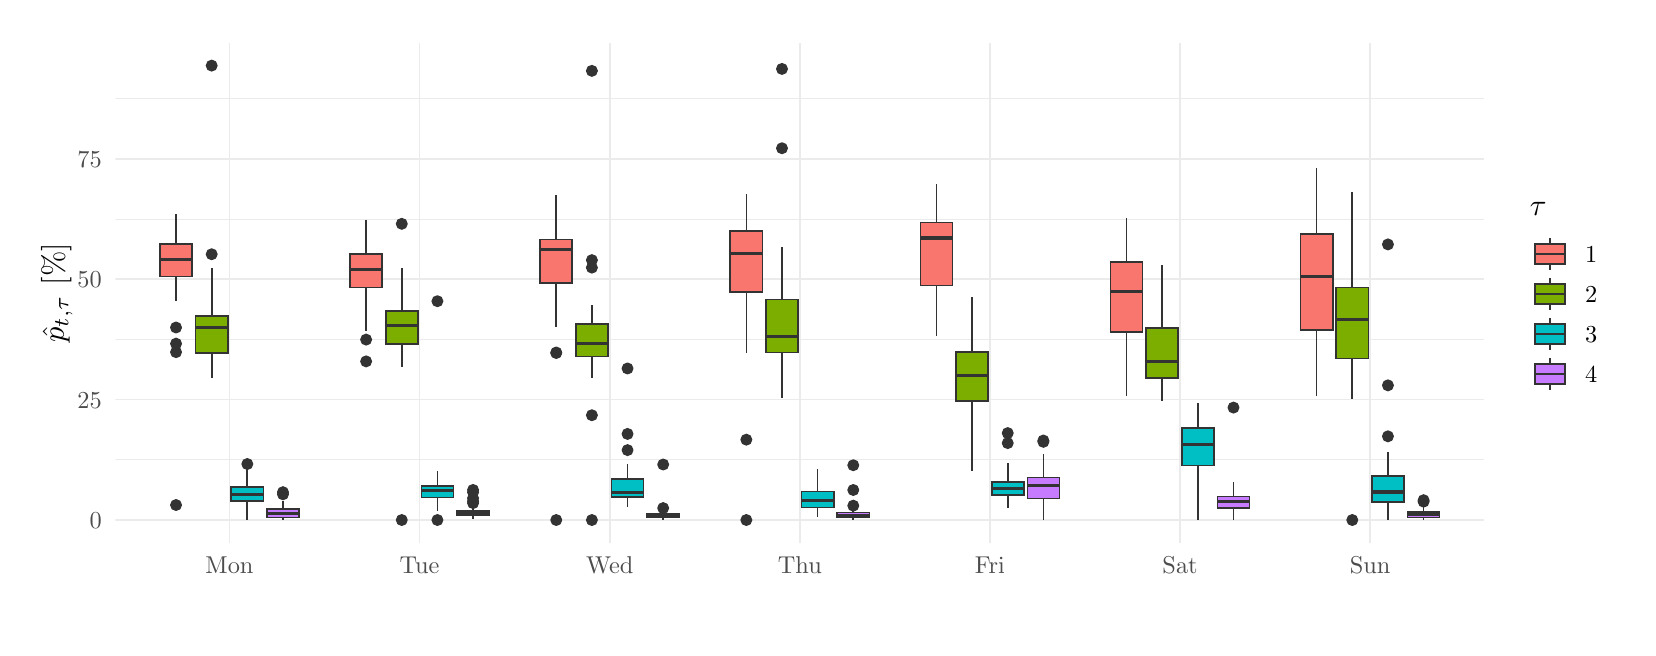
\begin{tikzpicture}[x=1pt,y=1pt]
\definecolor{fillColor}{RGB}{255,255,255}
\path[use as bounding box,fill=fillColor,fill opacity=0.00] (0,0) rectangle (578.16,216.81);
\begin{scope}
\path[clip] ( 31.71, 30.69) rectangle (526.31,211.31);
\definecolor{drawColor}{gray}{0.92}

\path[draw=drawColor,line width= 0.3pt,line join=round] ( 31.71, 60.64) --
	(526.31, 60.64);

\path[draw=drawColor,line width= 0.3pt,line join=round] ( 31.71,104.13) --
	(526.31,104.13);

\path[draw=drawColor,line width= 0.3pt,line join=round] ( 31.71,147.62) --
	(526.31,147.62);

\path[draw=drawColor,line width= 0.3pt,line join=round] ( 31.71,191.11) --
	(526.31,191.11);

\path[draw=drawColor,line width= 0.6pt,line join=round] ( 31.71, 38.90) --
	(526.31, 38.90);

\path[draw=drawColor,line width= 0.6pt,line join=round] ( 31.71, 82.39) --
	(526.31, 82.39);

\path[draw=drawColor,line width= 0.6pt,line join=round] ( 31.71,125.88) --
	(526.31,125.88);

\path[draw=drawColor,line width= 0.6pt,line join=round] ( 31.71,169.36) --
	(526.31,169.36);

\path[draw=drawColor,line width= 0.6pt,line join=round] ( 72.93, 30.69) --
	( 72.93,211.31);

\path[draw=drawColor,line width= 0.6pt,line join=round] (141.62, 30.69) --
	(141.62,211.31);

\path[draw=drawColor,line width= 0.6pt,line join=round] (210.32, 30.69) --
	(210.32,211.31);

\path[draw=drawColor,line width= 0.6pt,line join=round] (279.01, 30.69) --
	(279.01,211.31);

\path[draw=drawColor,line width= 0.6pt,line join=round] (347.70, 30.69) --
	(347.70,211.31);

\path[draw=drawColor,line width= 0.6pt,line join=round] (416.40, 30.69) --
	(416.40,211.31);

\path[draw=drawColor,line width= 0.6pt,line join=round] (485.09, 30.69) --
	(485.09,211.31);
\definecolor{drawColor}{gray}{0.20}
\definecolor{fillColor}{gray}{0.20}

\path[draw=drawColor,line width= 0.4pt,line join=round,line cap=round,fill=fillColor] ( 53.61,108.46) circle (  1.96);

\path[draw=drawColor,line width= 0.4pt,line join=round,line cap=round,fill=fillColor] ( 53.61,102.63) circle (  1.96);

\path[draw=drawColor,line width= 0.4pt,line join=round,line cap=round,fill=fillColor] ( 53.61, 99.56) circle (  1.96);

\path[draw=drawColor,line width= 0.4pt,line join=round,line cap=round,fill=fillColor] ( 53.61, 44.32) circle (  1.96);

\path[draw=drawColor,line width= 0.6pt,line join=round] ( 53.61,138.67) -- ( 53.61,149.60);

\path[draw=drawColor,line width= 0.6pt,line join=round] ( 53.61,126.86) -- ( 53.61,118.04);
\definecolor{fillColor}{RGB}{248,118,109}

\path[draw=drawColor,line width= 0.6pt,fill=fillColor] ( 47.81,138.67) --
	( 47.81,126.86) --
	( 59.40,126.86) --
	( 59.40,138.67) --
	( 47.81,138.67) --
	cycle;

\path[draw=drawColor,line width= 1.1pt] ( 47.81,133.04) -- ( 59.40,133.04);
\definecolor{fillColor}{gray}{0.20}

\path[draw=drawColor,line width= 0.4pt,line join=round,line cap=round,fill=fillColor] ( 66.49,134.94) circle (  1.96);

\path[draw=drawColor,line width= 0.4pt,line join=round,line cap=round,fill=fillColor] ( 66.49,203.10) circle (  1.96);

\path[draw=drawColor,line width= 0.6pt,line join=round] ( 66.49,112.55) -- ( 66.49,129.94);

\path[draw=drawColor,line width= 0.6pt,line join=round] ( 66.49, 99.20) -- ( 66.49, 90.37);
\definecolor{fillColor}{RGB}{124,174,0}

\path[draw=drawColor,line width= 0.6pt,fill=fillColor] ( 60.69,112.55) --
	( 60.69, 99.20) --
	( 72.28, 99.20) --
	( 72.28,112.55) --
	( 60.69,112.55) --
	cycle;

\path[draw=drawColor,line width= 1.1pt] ( 60.69,108.36) -- ( 72.28,108.36);
\definecolor{fillColor}{gray}{0.20}

\path[draw=drawColor,line width= 0.4pt,line join=round,line cap=round,fill=fillColor] ( 79.37, 59.14) circle (  1.96);

\path[draw=drawColor,line width= 0.6pt,line join=round] ( 79.37, 50.73) -- ( 79.37, 58.08);

\path[draw=drawColor,line width= 0.6pt,line join=round] ( 79.37, 45.68) -- ( 79.37, 38.90);
\definecolor{fillColor}{RGB}{0,191,196}

\path[draw=drawColor,line width= 0.6pt,fill=fillColor] ( 73.57, 50.73) --
	( 73.57, 45.68) --
	( 85.16, 45.68) --
	( 85.16, 50.73) --
	( 73.57, 50.73) --
	cycle;

\path[draw=drawColor,line width= 1.1pt] ( 73.57, 48.05) -- ( 85.16, 48.05);
\definecolor{fillColor}{gray}{0.20}

\path[draw=drawColor,line width= 0.4pt,line join=round,line cap=round,fill=fillColor] ( 92.25, 48.96) circle (  1.96);

\path[draw=drawColor,line width= 0.4pt,line join=round,line cap=round,fill=fillColor] ( 92.25, 48.19) circle (  1.96);

\path[draw=drawColor,line width= 0.6pt,line join=round] ( 92.25, 42.79) -- ( 92.25, 45.95);

\path[draw=drawColor,line width= 0.6pt,line join=round] ( 92.25, 39.80) -- ( 92.25, 38.90);
\definecolor{fillColor}{RGB}{199,124,255}

\path[draw=drawColor,line width= 0.6pt,fill=fillColor] ( 86.45, 42.79) --
	( 86.45, 39.80) --
	( 98.04, 39.80) --
	( 98.04, 42.79) --
	( 86.45, 42.79) --
	cycle;

\path[draw=drawColor,line width= 1.1pt] ( 86.45, 41.36) -- ( 98.04, 41.36);
\definecolor{fillColor}{gray}{0.20}

\path[draw=drawColor,line width= 0.4pt,line join=round,line cap=round,fill=fillColor] (122.30,104.09) circle (  1.96);

\path[draw=drawColor,line width= 0.4pt,line join=round,line cap=round,fill=fillColor] (122.30, 96.22) circle (  1.96);

\path[draw=drawColor,line width= 0.6pt,line join=round] (122.30,135.14) -- (122.30,147.36);

\path[draw=drawColor,line width= 0.6pt,line join=round] (122.30,122.87) -- (122.30,107.08);
\definecolor{fillColor}{RGB}{248,118,109}

\path[draw=drawColor,line width= 0.6pt,fill=fillColor] (116.51,135.14) --
	(116.51,122.87) --
	(128.10,122.87) --
	(128.10,135.14) --
	(116.51,135.14) --
	cycle;

\path[draw=drawColor,line width= 1.1pt] (116.51,129.28) -- (128.10,129.28);
\definecolor{fillColor}{gray}{0.20}

\path[draw=drawColor,line width= 0.4pt,line join=round,line cap=round,fill=fillColor] (135.18,145.93) circle (  1.96);

\path[draw=drawColor,line width= 0.4pt,line join=round,line cap=round,fill=fillColor] (135.18, 38.90) circle (  1.96);

\path[draw=drawColor,line width= 0.6pt,line join=round] (135.18,114.54) -- (135.18,130.07);

\path[draw=drawColor,line width= 0.6pt,line join=round] (135.18,102.42) -- (135.18, 94.15);
\definecolor{fillColor}{RGB}{124,174,0}

\path[draw=drawColor,line width= 0.6pt,fill=fillColor] (129.39,114.54) --
	(129.39,102.42) --
	(140.98,102.42) --
	(140.98,114.54) --
	(129.39,114.54) --
	cycle;

\path[draw=drawColor,line width= 1.1pt] (129.39,109.02) -- (140.98,109.02);
\definecolor{fillColor}{gray}{0.20}

\path[draw=drawColor,line width= 0.4pt,line join=round,line cap=round,fill=fillColor] (148.06,117.97) circle (  1.96);

\path[draw=drawColor,line width= 0.4pt,line join=round,line cap=round,fill=fillColor] (148.06, 38.90) circle (  1.96);

\path[draw=drawColor,line width= 0.6pt,line join=round] (148.06, 51.13) -- (148.06, 56.72);

\path[draw=drawColor,line width= 0.6pt,line join=round] (148.06, 47.00) -- (148.06, 42.04);
\definecolor{fillColor}{RGB}{0,191,196}

\path[draw=drawColor,line width= 0.6pt,fill=fillColor] (142.27, 51.13) --
	(142.27, 47.00) --
	(153.86, 47.00) --
	(153.86, 51.13) --
	(142.27, 51.13) --
	cycle;

\path[draw=drawColor,line width= 1.1pt] (142.27, 49.43) -- (153.86, 49.43);
\definecolor{fillColor}{gray}{0.20}

\path[draw=drawColor,line width= 0.4pt,line join=round,line cap=round,fill=fillColor] (160.94, 48.93) circle (  1.96);

\path[draw=drawColor,line width= 0.4pt,line join=round,line cap=round,fill=fillColor] (160.94, 49.77) circle (  1.96);

\path[draw=drawColor,line width= 0.4pt,line join=round,line cap=round,fill=fillColor] (160.94, 46.79) circle (  1.96);

\path[draw=drawColor,line width= 0.4pt,line join=round,line cap=round,fill=fillColor] (160.94, 45.01) circle (  1.96);

\path[draw=drawColor,line width= 0.4pt,line join=round,line cap=round,fill=fillColor] (160.94, 45.72) circle (  1.96);

\path[draw=drawColor,line width= 0.6pt,line join=round] (160.94, 42.16) -- (160.94, 44.42);

\path[draw=drawColor,line width= 0.6pt,line join=round] (160.94, 40.56) -- (160.94, 39.10);
\definecolor{fillColor}{RGB}{199,124,255}

\path[draw=drawColor,line width= 0.6pt,fill=fillColor] (155.15, 42.16) --
	(155.15, 40.56) --
	(166.74, 40.56) --
	(166.74, 42.16) --
	(155.15, 42.16) --
	cycle;

\path[draw=drawColor,line width= 1.1pt] (155.15, 41.22) -- (166.74, 41.22);
\definecolor{fillColor}{gray}{0.20}

\path[draw=drawColor,line width= 0.4pt,line join=round,line cap=round,fill=fillColor] (191.00, 99.43) circle (  1.96);

\path[draw=drawColor,line width= 0.4pt,line join=round,line cap=round,fill=fillColor] (191.00, 99.25) circle (  1.96);

\path[draw=drawColor,line width= 0.4pt,line join=round,line cap=round,fill=fillColor] (191.00, 38.90) circle (  1.96);

\path[draw=drawColor,line width= 0.6pt,line join=round] (191.00,140.27) -- (191.00,156.21);

\path[draw=drawColor,line width= 0.6pt,line join=round] (191.00,124.46) -- (191.00,108.72);
\definecolor{fillColor}{RGB}{248,118,109}

\path[draw=drawColor,line width= 0.6pt,fill=fillColor] (185.20,140.27) --
	(185.20,124.46) --
	(196.79,124.46) --
	(196.79,140.27) --
	(185.20,140.27) --
	cycle;

\path[draw=drawColor,line width= 1.1pt] (185.20,136.51) -- (196.79,136.51);
\definecolor{fillColor}{gray}{0.20}

\path[draw=drawColor,line width= 0.4pt,line join=round,line cap=round,fill=fillColor] (203.88,130.11) circle (  1.96);

\path[draw=drawColor,line width= 0.4pt,line join=round,line cap=round,fill=fillColor] (203.88,132.81) circle (  1.96);

\path[draw=drawColor,line width= 0.4pt,line join=round,line cap=round,fill=fillColor] (203.88, 76.77) circle (  1.96);

\path[draw=drawColor,line width= 0.4pt,line join=round,line cap=round,fill=fillColor] (203.88,201.20) circle (  1.96);

\path[draw=drawColor,line width= 0.4pt,line join=round,line cap=round,fill=fillColor] (203.88, 38.90) circle (  1.96);

\path[draw=drawColor,line width= 0.6pt,line join=round] (203.88,109.68) -- (203.88,116.57);

\path[draw=drawColor,line width= 0.6pt,line join=round] (203.88, 98.01) -- (203.88, 90.22);
\definecolor{fillColor}{RGB}{124,174,0}

\path[draw=drawColor,line width= 0.6pt,fill=fillColor] (198.08,109.68) --
	(198.08, 98.01) --
	(209.67, 98.01) --
	(209.67,109.68) --
	(198.08,109.68) --
	cycle;

\path[draw=drawColor,line width= 1.1pt] (198.08,102.76) -- (209.67,102.76);
\definecolor{fillColor}{gray}{0.20}

\path[draw=drawColor,line width= 0.4pt,line join=round,line cap=round,fill=fillColor] (216.76, 64.16) circle (  1.96);

\path[draw=drawColor,line width= 0.4pt,line join=round,line cap=round,fill=fillColor] (216.76, 70.01) circle (  1.96);

\path[draw=drawColor,line width= 0.4pt,line join=round,line cap=round,fill=fillColor] (216.76, 93.66) circle (  1.96);

\path[draw=drawColor,line width= 0.6pt,line join=round] (216.76, 53.72) -- (216.76, 59.24);

\path[draw=drawColor,line width= 0.6pt,line join=round] (216.76, 47.22) -- (216.76, 43.53);
\definecolor{fillColor}{RGB}{0,191,196}

\path[draw=drawColor,line width= 0.6pt,fill=fillColor] (210.96, 53.72) --
	(210.96, 47.22) --
	(222.55, 47.22) --
	(222.55, 53.72) --
	(210.96, 53.72) --
	cycle;

\path[draw=drawColor,line width= 1.1pt] (210.96, 48.99) -- (222.55, 48.99);
\definecolor{fillColor}{gray}{0.20}

\path[draw=drawColor,line width= 0.4pt,line join=round,line cap=round,fill=fillColor] (229.64, 58.96) circle (  1.96);

\path[draw=drawColor,line width= 0.4pt,line join=round,line cap=round,fill=fillColor] (229.64, 43.21) circle (  1.96);

\path[draw=drawColor,line width= 0.6pt,line join=round] (229.64, 41.12) -- (229.64, 42.34);

\path[draw=drawColor,line width= 0.6pt,line join=round] (229.64, 39.90) -- (229.64, 38.90);
\definecolor{fillColor}{RGB}{199,124,255}

\path[draw=drawColor,line width= 0.6pt,fill=fillColor] (223.84, 41.12) --
	(223.84, 39.90) --
	(235.43, 39.90) --
	(235.43, 41.12) --
	(223.84, 41.12) --
	cycle;

\path[draw=drawColor,line width= 1.1pt] (223.84, 40.45) -- (235.43, 40.45);
\definecolor{fillColor}{gray}{0.20}

\path[draw=drawColor,line width= 0.4pt,line join=round,line cap=round,fill=fillColor] (259.69, 67.93) circle (  1.96);

\path[draw=drawColor,line width= 0.4pt,line join=round,line cap=round,fill=fillColor] (259.69, 38.90) circle (  1.96);

\path[draw=drawColor,line width= 0.6pt,line join=round] (259.69,143.45) -- (259.69,156.54);

\path[draw=drawColor,line width= 0.6pt,line join=round] (259.69,121.36) -- (259.69, 99.37);
\definecolor{fillColor}{RGB}{248,118,109}

\path[draw=drawColor,line width= 0.6pt,fill=fillColor] (253.89,143.45) --
	(253.89,121.36) --
	(265.49,121.36) --
	(265.49,143.45) --
	(253.89,143.45) --
	cycle;

\path[draw=drawColor,line width= 1.1pt] (253.89,135.11) -- (265.49,135.11);
\definecolor{fillColor}{gray}{0.20}

\path[draw=drawColor,line width= 0.4pt,line join=round,line cap=round,fill=fillColor] (272.57,173.24) circle (  1.96);

\path[draw=drawColor,line width= 0.4pt,line join=round,line cap=round,fill=fillColor] (272.57,201.90) circle (  1.96);

\path[draw=drawColor,line width= 0.6pt,line join=round] (272.57,118.55) -- (272.57,137.57);

\path[draw=drawColor,line width= 0.6pt,line join=round] (272.57, 99.49) -- (272.57, 82.99);
\definecolor{fillColor}{RGB}{124,174,0}

\path[draw=drawColor,line width= 0.6pt,fill=fillColor] (266.77,118.55) --
	(266.77, 99.49) --
	(278.37, 99.49) --
	(278.37,118.55) --
	(266.77,118.55) --
	cycle;

\path[draw=drawColor,line width= 1.1pt] (266.77,105.38) -- (278.37,105.38);

\path[draw=drawColor,line width= 0.6pt,line join=round] (285.45, 49.23) -- (285.45, 57.20);

\path[draw=drawColor,line width= 0.6pt,line join=round] (285.45, 43.42) -- (285.45, 39.88);
\definecolor{fillColor}{RGB}{0,191,196}

\path[draw=drawColor,line width= 0.6pt,fill=fillColor] (279.65, 49.23) --
	(279.65, 43.42) --
	(291.25, 43.42) --
	(291.25, 49.23) --
	(279.65, 49.23) --
	cycle;

\path[draw=drawColor,line width= 1.1pt] (279.65, 45.80) -- (291.25, 45.80);
\definecolor{fillColor}{gray}{0.20}

\path[draw=drawColor,line width= 0.4pt,line join=round,line cap=round,fill=fillColor] (298.33, 44.09) circle (  1.96);

\path[draw=drawColor,line width= 0.4pt,line join=round,line cap=round,fill=fillColor] (298.33, 49.75) circle (  1.96);

\path[draw=drawColor,line width= 0.4pt,line join=round,line cap=round,fill=fillColor] (298.33, 58.70) circle (  1.96);

\path[draw=drawColor,line width= 0.6pt,line join=round] (298.33, 41.66) -- (298.33, 43.75);

\path[draw=drawColor,line width= 0.6pt,line join=round] (298.33, 40.06) -- (298.33, 38.90);
\definecolor{fillColor}{RGB}{199,124,255}

\path[draw=drawColor,line width= 0.6pt,fill=fillColor] (292.53, 41.66) --
	(292.53, 40.06) --
	(304.13, 40.06) --
	(304.13, 41.66) --
	(292.53, 41.66) --
	cycle;

\path[draw=drawColor,line width= 1.1pt] (292.53, 40.70) -- (304.13, 40.70);

\path[draw=drawColor,line width= 0.6pt,line join=round] (328.38,146.40) -- (328.38,160.14);

\path[draw=drawColor,line width= 0.6pt,line join=round] (328.38,123.66) -- (328.38,105.35);
\definecolor{fillColor}{RGB}{248,118,109}

\path[draw=drawColor,line width= 0.6pt,fill=fillColor] (322.59,146.40) --
	(322.59,123.66) --
	(334.18,123.66) --
	(334.18,146.40) --
	(322.59,146.40) --
	cycle;

\path[draw=drawColor,line width= 1.1pt] (322.59,140.80) -- (334.18,140.80);

\path[draw=drawColor,line width= 0.6pt,line join=round] (341.26, 99.65) -- (341.26,119.60);

\path[draw=drawColor,line width= 0.6pt,line join=round] (341.26, 81.98) -- (341.26, 56.47);
\definecolor{fillColor}{RGB}{124,174,0}

\path[draw=drawColor,line width= 0.6pt,fill=fillColor] (335.47, 99.65) --
	(335.47, 81.98) --
	(347.06, 81.98) --
	(347.06, 99.65) --
	(335.47, 99.65) --
	cycle;

\path[draw=drawColor,line width= 1.1pt] (335.47, 91.20) -- (347.06, 91.20);
\definecolor{fillColor}{gray}{0.20}

\path[draw=drawColor,line width= 0.4pt,line join=round,line cap=round,fill=fillColor] (354.14, 66.70) circle (  1.96);

\path[draw=drawColor,line width= 0.4pt,line join=round,line cap=round,fill=fillColor] (354.14, 70.31) circle (  1.96);

\path[draw=drawColor,line width= 0.6pt,line join=round] (354.14, 52.68) -- (354.14, 59.36);

\path[draw=drawColor,line width= 0.6pt,line join=round] (354.14, 47.97) -- (354.14, 43.12);
\definecolor{fillColor}{RGB}{0,191,196}

\path[draw=drawColor,line width= 0.6pt,fill=fillColor] (348.35, 52.68) --
	(348.35, 47.97) --
	(359.94, 47.97) --
	(359.94, 52.68) --
	(348.35, 52.68) --
	cycle;

\path[draw=drawColor,line width= 1.1pt] (348.35, 50.20) -- (359.94, 50.20);
\definecolor{fillColor}{gray}{0.20}

\path[draw=drawColor,line width= 0.4pt,line join=round,line cap=round,fill=fillColor] (367.02, 67.15) circle (  1.96);

\path[draw=drawColor,line width= 0.4pt,line join=round,line cap=round,fill=fillColor] (367.02, 67.63) circle (  1.96);

\path[draw=drawColor,line width= 0.6pt,line join=round] (367.02, 54.31) -- (367.02, 62.79);

\path[draw=drawColor,line width= 0.6pt,line join=round] (367.02, 46.69) -- (367.02, 38.90);
\definecolor{fillColor}{RGB}{199,124,255}

\path[draw=drawColor,line width= 0.6pt,fill=fillColor] (361.23, 54.31) --
	(361.23, 46.69) --
	(372.82, 46.69) --
	(372.82, 54.31) --
	(361.23, 54.31) --
	cycle;

\path[draw=drawColor,line width= 1.1pt] (361.23, 51.51) -- (372.82, 51.51);

\path[draw=drawColor,line width= 0.6pt,line join=round] (397.08,132.11) -- (397.08,147.94);

\path[draw=drawColor,line width= 0.6pt,line join=round] (397.08,106.78) -- (397.08, 83.54);
\definecolor{fillColor}{RGB}{248,118,109}

\path[draw=drawColor,line width= 0.6pt,fill=fillColor] (391.28,132.11) --
	(391.28,106.78) --
	(402.87,106.78) --
	(402.87,132.11) --
	(391.28,132.11) --
	cycle;

\path[draw=drawColor,line width= 1.1pt] (391.28,121.56) -- (402.87,121.56);

\path[draw=drawColor,line width= 0.6pt,line join=round] (409.96,108.34) -- (409.96,131.15);

\path[draw=drawColor,line width= 0.6pt,line join=round] (409.96, 90.28) -- (409.96, 81.74);
\definecolor{fillColor}{RGB}{124,174,0}

\path[draw=drawColor,line width= 0.6pt,fill=fillColor] (404.16,108.34) --
	(404.16, 90.28) --
	(415.75, 90.28) --
	(415.75,108.34) --
	(404.16,108.34) --
	cycle;

\path[draw=drawColor,line width= 1.1pt] (404.16, 96.26) -- (415.75, 96.26);

\path[draw=drawColor,line width= 0.6pt,line join=round] (422.84, 72.12) -- (422.84, 81.35);

\path[draw=drawColor,line width= 0.6pt,line join=round] (422.84, 58.64) -- (422.84, 38.90);
\definecolor{fillColor}{RGB}{0,191,196}

\path[draw=drawColor,line width= 0.6pt,fill=fillColor] (417.04, 72.12) --
	(417.04, 58.64) --
	(428.63, 58.64) --
	(428.63, 72.12) --
	(417.04, 72.12) --
	cycle;

\path[draw=drawColor,line width= 1.1pt] (417.04, 66.08) -- (428.63, 66.08);
\definecolor{fillColor}{gray}{0.20}

\path[draw=drawColor,line width= 0.4pt,line join=round,line cap=round,fill=fillColor] (435.72, 79.53) circle (  1.96);

\path[draw=drawColor,line width= 0.6pt,line join=round] (435.72, 47.42) -- (435.72, 52.60);

\path[draw=drawColor,line width= 0.6pt,line join=round] (435.72, 43.26) -- (435.72, 38.90);
\definecolor{fillColor}{RGB}{199,124,255}

\path[draw=drawColor,line width= 0.6pt,fill=fillColor] (429.92, 47.42) --
	(429.92, 43.26) --
	(441.51, 43.26) --
	(441.51, 47.42) --
	(429.92, 47.42) --
	cycle;

\path[draw=drawColor,line width= 1.1pt] (429.92, 45.46) -- (441.51, 45.46);

\path[draw=drawColor,line width= 0.6pt,line join=round] (465.77,142.34) -- (465.77,165.99);

\path[draw=drawColor,line width= 0.6pt,line join=round] (465.77,107.53) -- (465.77, 83.76);
\definecolor{fillColor}{RGB}{248,118,109}

\path[draw=drawColor,line width= 0.6pt,fill=fillColor] (459.97,142.34) --
	(459.97,107.53) --
	(471.57,107.53) --
	(471.57,142.34) --
	(459.97,142.34) --
	cycle;

\path[draw=drawColor,line width= 1.1pt] (459.97,126.95) -- (471.57,126.95);
\definecolor{fillColor}{gray}{0.20}

\path[draw=drawColor,line width= 0.4pt,line join=round,line cap=round,fill=fillColor] (478.65, 38.90) circle (  1.96);

\path[draw=drawColor,line width= 0.6pt,line join=round] (478.65,122.90) -- (478.65,157.31);

\path[draw=drawColor,line width= 0.6pt,line join=round] (478.65, 97.22) -- (478.65, 82.58);
\definecolor{fillColor}{RGB}{124,174,0}

\path[draw=drawColor,line width= 0.6pt,fill=fillColor] (472.85,122.90) --
	(472.85, 97.22) --
	(484.45, 97.22) --
	(484.45,122.90) --
	(472.85,122.90) --
	cycle;

\path[draw=drawColor,line width= 1.1pt] (472.85,111.47) -- (484.45,111.47);
\definecolor{fillColor}{gray}{0.20}

\path[draw=drawColor,line width= 0.4pt,line join=round,line cap=round,fill=fillColor] (491.53, 87.56) circle (  1.96);

\path[draw=drawColor,line width= 0.4pt,line join=round,line cap=round,fill=fillColor] (491.53,138.49) circle (  1.96);

\path[draw=drawColor,line width= 0.4pt,line join=round,line cap=round,fill=fillColor] (491.53, 69.14) circle (  1.96);

\path[draw=drawColor,line width= 0.6pt,line join=round] (491.53, 54.70) -- (491.53, 63.51);

\path[draw=drawColor,line width= 0.6pt,line join=round] (491.53, 45.38) -- (491.53, 38.90);
\definecolor{fillColor}{RGB}{0,191,196}

\path[draw=drawColor,line width= 0.6pt,fill=fillColor] (485.73, 54.70) --
	(485.73, 45.38) --
	(497.33, 45.38) --
	(497.33, 54.70) --
	(485.73, 54.70) --
	cycle;

\path[draw=drawColor,line width= 1.1pt] (485.73, 49.03) -- (497.33, 49.03);
\definecolor{fillColor}{gray}{0.20}

\path[draw=drawColor,line width= 0.4pt,line join=round,line cap=round,fill=fillColor] (504.41, 46.07) circle (  1.96);

\path[draw=drawColor,line width= 0.4pt,line join=round,line cap=round,fill=fillColor] (504.41, 45.54) circle (  1.96);

\path[draw=drawColor,line width= 0.6pt,line join=round] (504.41, 41.73) -- (504.41, 43.83);

\path[draw=drawColor,line width= 0.6pt,line join=round] (504.41, 39.85) -- (504.41, 38.90);
\definecolor{fillColor}{RGB}{199,124,255}

\path[draw=drawColor,line width= 0.6pt,fill=fillColor] (498.61, 41.73) --
	(498.61, 39.85) --
	(510.21, 39.85) --
	(510.21, 41.73) --
	(498.61, 41.73) --
	cycle;

\path[draw=drawColor,line width= 1.1pt] (498.61, 40.90) -- (510.21, 40.90);
\end{scope}
\begin{scope}
\path[clip] (  0.00,  0.00) rectangle (578.16,216.81);
\definecolor{drawColor}{gray}{0.30}

\node[text=drawColor,anchor=base east,inner sep=0pt, outer sep=0pt, scale=  0.88] at ( 26.76, 35.87) {0};

\node[text=drawColor,anchor=base east,inner sep=0pt, outer sep=0pt, scale=  0.88] at ( 26.76, 79.36) {25};

\node[text=drawColor,anchor=base east,inner sep=0pt, outer sep=0pt, scale=  0.88] at ( 26.76,122.84) {50};

\node[text=drawColor,anchor=base east,inner sep=0pt, outer sep=0pt, scale=  0.88] at ( 26.76,166.33) {75};
\end{scope}
\begin{scope}
\path[clip] (  0.00,  0.00) rectangle (578.16,216.81);
\definecolor{drawColor}{gray}{0.30}

\node[text=drawColor,anchor=base,inner sep=0pt, outer sep=0pt, scale=  0.88] at ( 72.93, 19.68) {Mon};

\node[text=drawColor,anchor=base,inner sep=0pt, outer sep=0pt, scale=  0.88] at (141.62, 19.68) {Tue};

\node[text=drawColor,anchor=base,inner sep=0pt, outer sep=0pt, scale=  0.88] at (210.32, 19.68) {Wed};

\node[text=drawColor,anchor=base,inner sep=0pt, outer sep=0pt, scale=  0.88] at (279.01, 19.68) {Thu};

\node[text=drawColor,anchor=base,inner sep=0pt, outer sep=0pt, scale=  0.88] at (347.70, 19.68) {Fri};

\node[text=drawColor,anchor=base,inner sep=0pt, outer sep=0pt, scale=  0.88] at (416.40, 19.68) {Sat};

\node[text=drawColor,anchor=base,inner sep=0pt, outer sep=0pt, scale=  0.88] at (485.09, 19.68) {Sun};
\end{scope}
\begin{scope}
\path[clip] (  0.00,  0.00) rectangle (578.16,216.81);
\definecolor{drawColor}{RGB}{0,0,0}

\node[text=drawColor,rotate= 90.00,anchor=base,inner sep=0pt, outer sep=0pt, scale=  1.10] at ( 13.08,121.00) {$\hat p_{t, \tau}$ [\%]};
\end{scope}
\begin{scope}
\path[clip] (  0.00,  0.00) rectangle (578.16,216.81);
\definecolor{drawColor}{RGB}{0,0,0}

\node[text=drawColor,anchor=base west,inner sep=0pt, outer sep=0pt, scale=  1.10] at (542.81,148.87) {$\tau$};
\end{scope}
\begin{scope}
\path[clip] (  0.00,  0.00) rectangle (578.16,216.81);
\definecolor{drawColor}{gray}{0.20}

\path[draw=drawColor,line width= 0.6pt] (550.03,129.29) --
	(550.03,131.46);

\path[draw=drawColor,line width= 0.6pt] (550.03,138.69) --
	(550.03,140.85);
\definecolor{fillColor}{RGB}{248,118,109}

\path[draw=drawColor,line width= 0.6pt,fill=fillColor] (544.61,131.46) rectangle (555.45,138.69);

\path[draw=drawColor,line width= 0.6pt] (544.61,135.07) --
	(555.45,135.07);
\end{scope}
\begin{scope}
\path[clip] (  0.00,  0.00) rectangle (578.16,216.81);
\definecolor{drawColor}{gray}{0.20}

\path[draw=drawColor,line width= 0.6pt] (550.03,114.84) --
	(550.03,117.00);

\path[draw=drawColor,line width= 0.6pt] (550.03,124.23) --
	(550.03,126.40);
\definecolor{fillColor}{RGB}{124,174,0}

\path[draw=drawColor,line width= 0.6pt,fill=fillColor] (544.61,117.00) rectangle (555.45,124.23);

\path[draw=drawColor,line width= 0.6pt] (544.61,120.62) --
	(555.45,120.62);
\end{scope}
\begin{scope}
\path[clip] (  0.00,  0.00) rectangle (578.16,216.81);
\definecolor{drawColor}{gray}{0.20}

\path[draw=drawColor,line width= 0.6pt] (550.03,100.38) --
	(550.03,102.55);

\path[draw=drawColor,line width= 0.6pt] (550.03,109.78) --
	(550.03,111.95);
\definecolor{fillColor}{RGB}{0,191,196}

\path[draw=drawColor,line width= 0.6pt,fill=fillColor] (544.61,102.55) rectangle (555.45,109.78);

\path[draw=drawColor,line width= 0.6pt] (544.61,106.16) --
	(555.45,106.16);
\end{scope}
\begin{scope}
\path[clip] (  0.00,  0.00) rectangle (578.16,216.81);
\definecolor{drawColor}{gray}{0.20}

\path[draw=drawColor,line width= 0.6pt] (550.03, 85.93) --
	(550.03, 88.10);

\path[draw=drawColor,line width= 0.6pt] (550.03, 95.32) --
	(550.03, 97.49);
\definecolor{fillColor}{RGB}{199,124,255}

\path[draw=drawColor,line width= 0.6pt,fill=fillColor] (544.61, 88.10) rectangle (555.45, 95.32);

\path[draw=drawColor,line width= 0.6pt] (544.61, 91.71) --
	(555.45, 91.71);
\end{scope}
\begin{scope}
\path[clip] (  0.00,  0.00) rectangle (578.16,216.81);
\definecolor{drawColor}{RGB}{0,0,0}

\node[text=drawColor,anchor=base west,inner sep=0pt, outer sep=0pt, scale=  0.88] at (562.76,132.04) {1};
\end{scope}
\begin{scope}
\path[clip] (  0.00,  0.00) rectangle (578.16,216.81);
\definecolor{drawColor}{RGB}{0,0,0}

\node[text=drawColor,anchor=base west,inner sep=0pt, outer sep=0pt, scale=  0.88] at (562.76,117.59) {2};
\end{scope}
\begin{scope}
\path[clip] (  0.00,  0.00) rectangle (578.16,216.81);
\definecolor{drawColor}{RGB}{0,0,0}

\node[text=drawColor,anchor=base west,inner sep=0pt, outer sep=0pt, scale=  0.88] at (562.76,103.13) {3};
\end{scope}
\begin{scope}
\path[clip] (  0.00,  0.00) rectangle (578.16,216.81);
\definecolor{drawColor}{RGB}{0,0,0}

\node[text=drawColor,anchor=base west,inner sep=0pt, outer sep=0pt, scale=  0.88] at (562.76, 88.68) {4};
\end{scope}
\end{tikzpicture}
%
    }
    \caption{Box plots of delay probabilities $\hat p_{t,\tau}$ by weekday of case reporting date $t$. As there are systematically fewer cases reported on Sunday, there is a small weekday effect: $p_{t,1}$ for Saturdays, $p_{t,2}$ for Fridays, $p_{t,3}$ for Thursdays and $p_{t,4}$ for Wednesdays are small compared to other days.}
    \label{fig:weekday_effect_delays}
\end{figure}

To produce accurate forecasts of the daily number of reported cases, we will construct a \acrshort{ssm} that allows to account for these delays, as well as the weekday effects and dynamics of the incidences. With this model, we will then perform short-term forecasts for the case incidence in Germany, including prediction intervals. To assess the performance of our method, we compare the results to those produced in the \acrfull{ecdc}'s ForecastHub \citep{Sherratt2022Predictive}.
%\todo{also remove reporting artifacts at christmas?}

\subsection{Model}

To model the development of cases over time, we start with the exponential growth equation \Cref{eq:exponential-growth-time-varying}. Let $I_{t}$ be the total number of cases for reporting date $t$, unaffected by weekday effects and reporting delays. Ignoring variation around the mean, the exponential growth ansatz gives 
$$
    \log I_{t + 1} \approx \log \rho_{t + 1}  + \log I_{t}
$$
for the growth factor $\rho_{t}$ on day $t$. It is then sensible to assume that the growth factor $\rho_{t}$ performs a random walk on the log-scale, as we would expect large day-to-day variation of $\rho_{t}$ for large values, and small variation for small values, i.e. multiplicative, rather than additive, day-to-day changes. Thus, we assume that 
$$
    \log \rho_{t + 1} = \rho_{t} + \varepsilon_{t + 1, \rho}
$$
for $\varepsilon_{t + 1,\rho} \sim \mathcal N(0, \sigma^{2}_\rho)$. To incorporate week-day effects, consider a weekly seasonal component 
$$
    \log W_{t + 1} = - \sum_{s = 0}^{5} \log W_{t - s} + \varepsilon_{t + 1, W},
$$
for $\varepsilon_{t + 1, W} \sim \mathcal N(0, \sigma^{2}_{W})$, as described in \Cref{sec:modelling_epidemiological_dessiderata_with_state_space_models}. Finally, to model the reporting delay probabilities $p_{t,\tau}$, $\tau = 1,2,3,4$, we parameterize them by log ratios
\begin{align*}
    q_{t, \tau} = \log \frac{p_{t,\tau}}{p_{t,4}} && \tau = 1,\dots, 3,
\end{align*}
which also perform a random walk in time: 
$$
    q_{t + 1, \tau} = q_{t, \tau} + \varepsilon_{t+1, q, \tau},
$$
with $\varepsilon_{t + 1, q, \tau} \sim \mathcal N(0, \sigma^{2}_{q})$ whose variance does not depend on the delay $\tau$. To account for the weekday effect visible in \Cref{fig:weekday_effect_delays}, we introduce three further weekday effects 
$$
    \log W^{q,\tau}_{t + 1} = - \sum_{s = 0}^{5} \log W^{q,\tau}_{t - s} + \varepsilon_{t + 1, W^{q,\tau}},
$$
with $\varepsilon_{t+1, W^{q,\tau}} \sim \mathcal N \left( 0, \sigma^{2}_{W_q} \right)$, with shared variance $\sigma^{2}_{W_{q}}$.
We can recover the delay probabilities $p_{t, \tau}$ from the log-ratios by 
\begin{align}
    \begin{split}
        \label{eq:p-from-log-ratios}
    p_{t, 4} &= \frac{1}{1 + \sum_{\tau = 1}^3 \exp \left( q_{t,\tau} + \log W^{q,\tau}_{t} \right)}, \\
    p_{t, \tau} &= \exp\left( q_{t, \tau + \log W^{q, \tau}_{t}} \right) p_{t, 4},
    \end{split}
\end{align}
for $\tau = 1, 2, 3$.

Finally, there are reporting artifacts and other effects that we have not yet considered in our model contribute to the dirtiness of the data. To account for these effects, we model daily, multiplicative, \glqq{}muck\grqq{} $M_{t}$, for date $t$, such that the total expected number of reported cases on this date is $M_{t}I_{t}$ instead of $I_{t}$. We assume that $(\log M_{t})_{t = 0, \dots, n} \iid \mathcal N(-\frac{1}{2}\sigma^{2}_M, \sigma^{2}_{M})$, independent of all other states. Thus, $M_{t}$ follows a log-normal distribution with mean $1$. 

With these components at our disposal, we can model the observed incidences $Y_{t, \tau}$ by
\begin{align}
    \label{eq:reporting_delays_Y}
    Y_{t, \tau} | \log I_{t}, \log W_{t}, q_{t}, \log M_{t} \sim \operatorname{Pois} \left( p_{t, \tau}\exp \left(\log I_{t} + \log W_{t}  + \log M_{t}\right) \right) = \operatorname{Pois} \left( p_{t, \tau} W_{t} M_{t} I_{t}\right),
\end{align}
conditionally independent for fixed $t$. Thus, $W_{t}$ acts as a multiplicative factor that modulates the observed cases depending on the day of the week, and the delay probabilities distribute the total expected number of cases $M_{t}W_{t}I_{t}$ onto the delays. In this model, $Y_{t} = \sum_{\tau = 1}^4 Y_{t, \tau}$ has conditional expectation 
$$
    \E \left( Y_{t} | \log I_{t}, \log W_{t}, q_{t}, \log M_{t} \right) = M_{t}W_{t}I_t
$$
As it is sensible to model the conditional distribution of $Y_{t}$ by a Poisson distribution (see \Cref{sec:dessiderata}), we can view \Cref{eq:reporting_delays_Y} as a multinomial thinning of this distribution. Notice that including $M_{t}$ introduces overdispersion in this Poisson distribution, similar to a negative binomial distribution. 

Letting $X_{t} =\left( \log I_{t}, \log \rho_{t + 1}, \log W_{t}, \dots, \log W_{t - 5}, q_{t,1}, q_{t,2}, q_{t,3}\right)^{T}$, assuming that
$$
\varepsilon_{t + 1} = 
\begin{pmatrix}
     \varepsilon_{t + 1,\rho}\\ \varepsilon_{t + 1, W}\\ \varepsilon_{t +1, q, 1}\\ \varepsilon_{t +1, q, 2}\\ \varepsilon_{t +1, q, 3}
\end{pmatrix}
$$
has independent marginals, and fixing an initial distribution of $X_{0}$ fully specifies a \acrshort{pgssm} for the joint distribution of $(X,Y)$. The model has a linear signal 
$$
    S_{t} = \begin{pmatrix}
        \log I_{t} + \log W_{t} \\
        q_{t, 1} \\
        q_{t, 2} \\
        q_{t, 3} 
    \end{pmatrix},
$$
but due to the non-linear dependence of $p_{t,\tau}$ on $q_{t,\tau}$,  $Y_{t,\tau}$ depends not just on $S_{t, \tau}$ but on the whole of $S_{t}$. Fortunately, this is not a problem for either the \acrshort{la} or \acrshort{eis}. For the \acrshort{la} (\Cref{alg:la}), notice that the covariance matrix $\Omega_{t}$ is given by the inverse of the negative Hessian of $s_{t} \mapsto \log p(y_{t}|s_{t})$, which is now non-diagonal. While it is not guaranteed that $\Omega_{t}$ is positive semi-definite during the Newton-Raphson iteration, we can still employ the Kalman filter and signal smoother to perform the iteration efficiently, see \citep{Jungbacker2007Monte} and the discussion in \Cref{subsec:glssm-approach}. Furthermore, at the global optimum, the Hessian is negative semi-definite, so $\Omega_{t}$ is positive semi-definite, specifying a valid \acrshort{glssm} proposal. 
Similarly, we may extend \acrshort{eis} to account for non-diagonal $\Omega_{t}$. Recall from \Cref{subsec:eis}, that \acrshort{eis} minimizes for a given $t$ 
$$
    \sum_{i = 1}^N \left( \log p(y_{t} | S^{i}_t) + \langle \Omega_{t}^{-1}z_{t}, S^{i}_{t}\rangle - \frac{1}{2} \operatorname{tr} \left(\Omega^{-1}_{t}S^{i}_{t}(S^{i}_t)^{T}\right)- \lambda_{t} \right)^{2}
$$
over $z_{t}, \Omega_{t}, \lambda_{t}$. Noticing that $(A,B) \mapsto \operatorname{tr} \left( A^{T}B \right)$ is the Frobenius inner-product, we see that this optimization problem is still a weighted linear least squares problem for $\Omega_{t}^{-1}z_{t}, \Omega^{-1}_t, \lambda_{t}$, when we let $\Omega_{t}^{-1}$ take values in the symmetric matrices in $\R^{p \times p}$. As the dimension of this vector space is $ \frac{p (p + 1)}{2}$, we may still perform the efficient weighted linear least squares routine, but at an increased cost: the number of parameters increases from $2p + 1$ ($\Omega_{t}$ diagonal) to $p + \frac{p(p + 1)}{2} + 1$ ($\Omega_{t}$ symmetric). 

The parameters of the model are $\theta = \left( \log \sigma^{2}_{\rho}, \log \sigma^{2}_{W}, \log \sigma^{2}_{q}, \log \sigma^{2}_M\right)$, which we model on the log-scale to avoid having to take care of constraints. Given observations $Y = (Y_{0}, \dots, Y_{n})$ we perform maximum likelihood estimation as described in \Cref{alg:mle}. As tuning parameters in this procedure we use $20$ iterations for the \acrshort{la} and \acrshort{eis}, with relative tolerance of convergence set to $10^{-5}$. For the \acrshort{eis} proposals we also use $1\,000$ samples and all four antithetic variables, i.e. we use \Cref{eq:antithetic-weights}. At the \acrshort{mle} we again determine the \acrshort{eis} proposal using the same parameters and perform inference for the conditional distribution using $10\,000$ samples, applying the method described in \Cref{subsec:inference} to obtain estimates of the posterior mean, standard deviation and prediction intervals. 

% results
\subsection{Results}
We start by a showcase of the models' capability, fitting it to the reported case date in the period from April 5th to September 1st 2020, starting from the first day when $4$ delays are available in the dataset to the initial period of exponential growth in the fall of 2020. We estimate the parameters $\theta = \left( \log \sigma^{2}_{\rho}, \log \sigma^{2}_W, \log \sigma^{2}_q, \log \sigma^{2}_M, \sigma^{2}_{W_{q}}\right)$ by maximum-likelihood estimation, yielding the parameters displayed in \Cref{tab:showcase-parameters}. There, we see that both $\log \rho_{t}$ and $\log W_{t}$ vary slowly over time, compared to the faster varying $q$. 

\begin{table}
    \centering
    
\begin{tabular}{lrrrrr}
\toprule
method & $\hat\sigma_{ \rho }$ & $\hat\sigma_{ W }$ & $\hat\sigma_{ q }$ & $\hat\sigma_{ M }$ & $\hat\sigma_{ W_q }$\\
\midrule
manual & 0.001 & 0.100 & 0.50 & 0.01 & 0.10\\
initial & 0.015 & 0.024 & 0.12 & 0.14 & 0.81\\
MLE & 0.015 & 0.024 & 0.12 & 0.14 & 0.81\\
\bottomrule
\end{tabular}
    \label{tab:showcase-parameters}
    \caption{Standard deviations for the showcase model determined either by hand, by the initial search or by maximum likelihood estimation described in \Cref{sec:maximum_likelihood_estimation}. The difference between the initial search and the \acrshort{mle} is negligible and is not visible for the precision shown here.}
\end{table}
\begin{figure}
    \resizebox{\textwidth}{!}{%
        % Created by tikzDevice version 0.12.6 on 2024-09-22 14:10:20
% !TEX encoding = UTF-8 Unicode
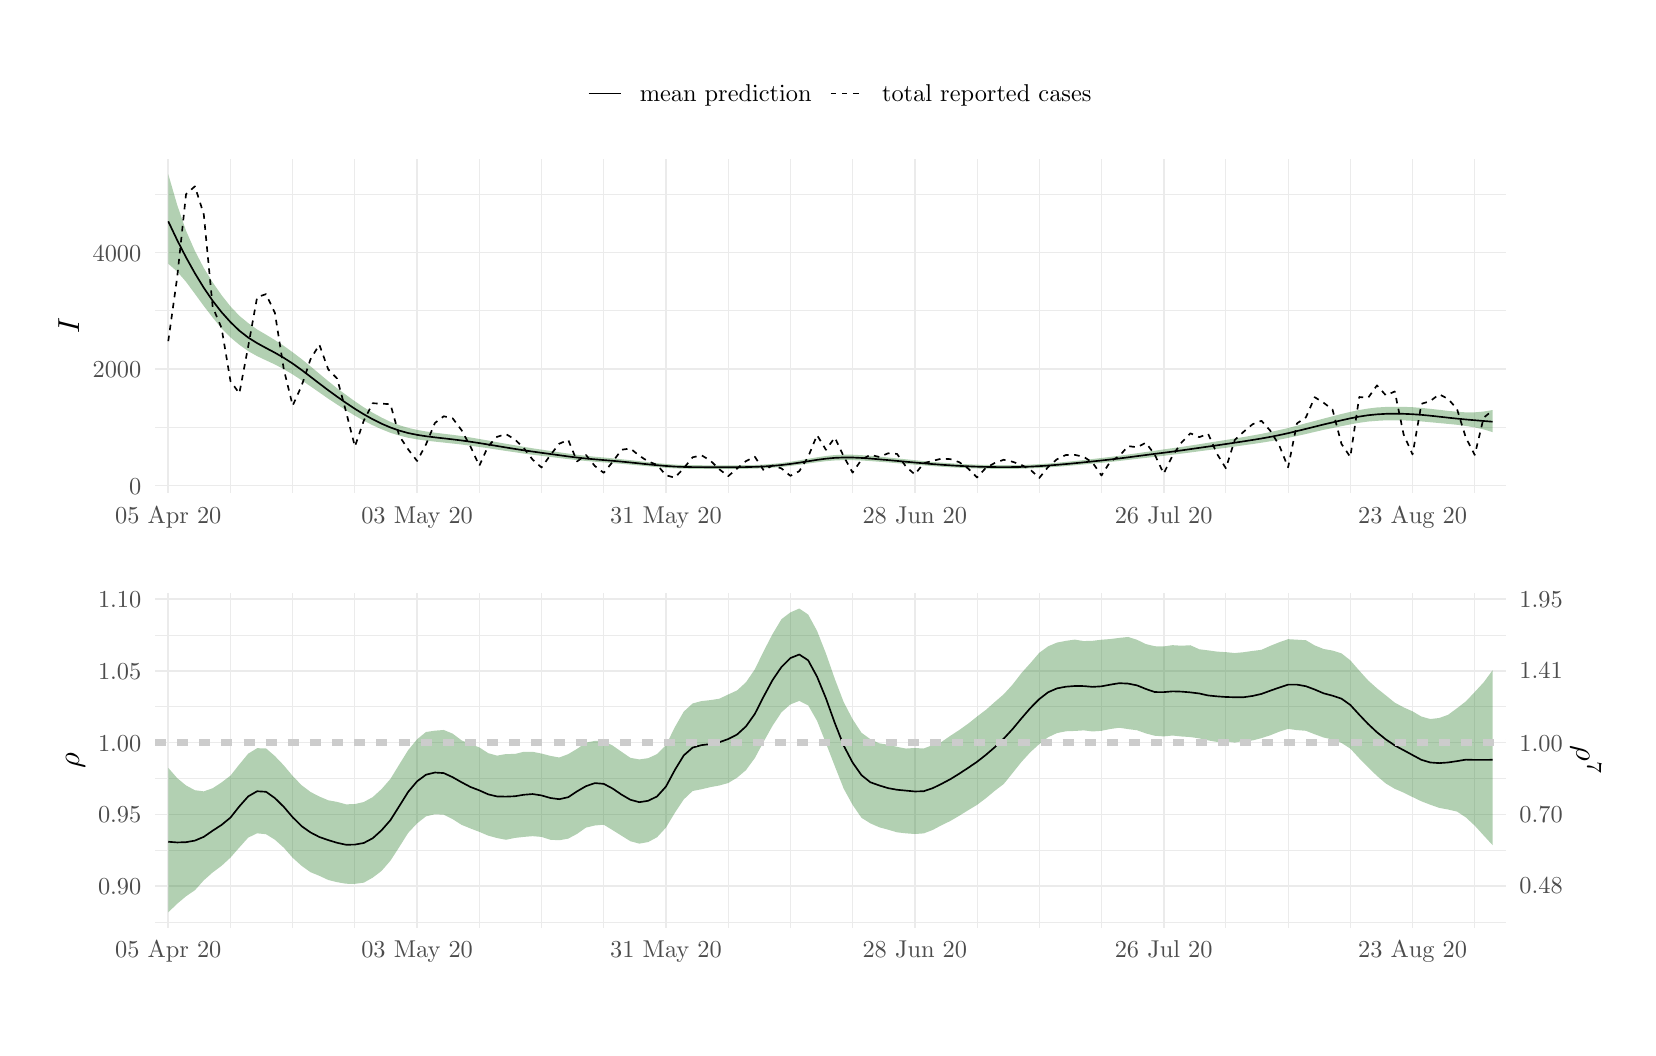
\begin{tikzpicture}[x=1pt,y=1pt]
\definecolor{fillColor}{RGB}{255,255,255}
\path[use as bounding box,fill=fillColor,fill opacity=0.00] (0,0) rectangle (578.16,361.35);
\begin{scope}
\path[clip] ( 46.01,193.13) rectangle (534.10,313.90);
\definecolor{drawColor}{gray}{0.92}

\path[draw=drawColor,line width= 0.3pt,line join=round] ( 46.01,216.91) --
	(534.10,216.91);

\path[draw=drawColor,line width= 0.3pt,line join=round] ( 46.01,259.01) --
	(534.10,259.01);

\path[draw=drawColor,line width= 0.3pt,line join=round] ( 46.01,301.11) --
	(534.10,301.11);

\path[draw=drawColor,line width= 0.3pt,line join=round] ( 73.28,193.13) --
	( 73.28,313.90);

\path[draw=drawColor,line width= 0.3pt,line join=round] ( 95.76,193.13) --
	( 95.76,313.90);

\path[draw=drawColor,line width= 0.3pt,line join=round] (118.24,193.13) --
	(118.24,313.90);

\path[draw=drawColor,line width= 0.3pt,line join=round] (163.20,193.13) --
	(163.20,313.90);

\path[draw=drawColor,line width= 0.3pt,line join=round] (185.68,193.13) --
	(185.68,313.90);

\path[draw=drawColor,line width= 0.3pt,line join=round] (208.16,193.13) --
	(208.16,313.90);

\path[draw=drawColor,line width= 0.3pt,line join=round] (253.12,193.13) --
	(253.12,313.90);

\path[draw=drawColor,line width= 0.3pt,line join=round] (275.61,193.13) --
	(275.61,313.90);

\path[draw=drawColor,line width= 0.3pt,line join=round] (298.09,193.13) --
	(298.09,313.90);

\path[draw=drawColor,line width= 0.3pt,line join=round] (343.05,193.13) --
	(343.05,313.90);

\path[draw=drawColor,line width= 0.3pt,line join=round] (365.53,193.13) --
	(365.53,313.90);

\path[draw=drawColor,line width= 0.3pt,line join=round] (388.01,193.13) --
	(388.01,313.90);

\path[draw=drawColor,line width= 0.3pt,line join=round] (432.97,193.13) --
	(432.97,313.90);

\path[draw=drawColor,line width= 0.3pt,line join=round] (455.45,193.13) --
	(455.45,313.90);

\path[draw=drawColor,line width= 0.3pt,line join=round] (477.93,193.13) --
	(477.93,313.90);

\path[draw=drawColor,line width= 0.3pt,line join=round] (522.90,193.13) --
	(522.90,313.90);

\path[draw=drawColor,line width= 0.6pt,line join=round] ( 46.01,195.87) --
	(534.10,195.87);

\path[draw=drawColor,line width= 0.6pt,line join=round] ( 46.01,237.96) --
	(534.10,237.96);

\path[draw=drawColor,line width= 0.6pt,line join=round] ( 46.01,280.06) --
	(534.10,280.06);

\path[draw=drawColor,line width= 0.6pt,line join=round] ( 50.80,193.13) --
	( 50.80,313.90);

\path[draw=drawColor,line width= 0.6pt,line join=round] (140.72,193.13) --
	(140.72,313.90);

\path[draw=drawColor,line width= 0.6pt,line join=round] (230.64,193.13) --
	(230.64,313.90);

\path[draw=drawColor,line width= 0.6pt,line join=round] (320.57,193.13) --
	(320.57,313.90);

\path[draw=drawColor,line width= 0.6pt,line join=round] (410.49,193.13) --
	(410.49,313.90);

\path[draw=drawColor,line width= 0.6pt,line join=round] (500.42,193.13) --
	(500.42,313.90);
\definecolor{fillColor}{RGB}{0,100,0}

\path[fill=fillColor,fill opacity=0.30] ( 50.80,308.41) --
	( 54.01,297.34) --
	( 57.22,287.98) --
	( 60.43,280.67) --
	( 63.64,274.53) --
	( 66.85,269.31) --
	( 70.06,264.70) --
	( 73.28,260.62) --
	( 76.49,257.24) --
	( 79.70,254.59) --
	( 82.91,252.30) --
	( 86.12,250.41) --
	( 89.33,248.47) --
	( 92.55,246.38) --
	( 95.76,244.04) --
	( 98.97,241.61) --
	(102.18,238.99) --
	(105.39,236.30) --
	(108.60,233.63) --
	(111.82,231.05) --
	(115.03,228.66) --
	(118.24,226.33) --
	(121.45,224.17) --
	(124.66,222.21) --
	(127.87,220.47) --
	(131.08,218.90) --
	(134.30,217.70) --
	(137.51,216.74) --
	(140.72,216.00) --
	(143.93,215.44) --
	(147.14,215.00) --
	(150.35,214.60) --
	(153.57,214.22) --
	(156.78,213.78) --
	(159.99,213.27) --
	(163.20,212.72) --
	(166.41,212.16) --
	(169.62,211.56) --
	(172.84,210.99) --
	(176.05,210.46) --
	(179.26,209.88) --
	(182.47,209.35) --
	(185.68,208.87) --
	(188.89,208.40) --
	(192.10,207.92) --
	(195.32,207.44) --
	(198.53,207.01) --
	(201.74,206.64) --
	(204.95,206.31) --
	(208.16,206.03) --
	(211.37,205.72) --
	(214.59,205.40) --
	(217.80,205.06) --
	(221.01,204.70) --
	(224.22,204.33) --
	(227.43,204.00) --
	(230.64,203.69) --
	(233.86,203.45) --
	(237.07,203.31) --
	(240.28,203.25) --
	(243.49,203.23) --
	(246.70,203.21) --
	(249.91,203.20) --
	(253.12,203.19) --
	(256.34,203.21) --
	(259.55,203.26) --
	(262.76,203.32) --
	(265.97,203.48) --
	(269.18,203.72) --
	(272.39,204.05) --
	(275.61,204.49) --
	(278.82,205.00) --
	(282.03,205.56) --
	(285.24,206.10) --
	(288.45,206.57) --
	(291.66,206.91) --
	(294.87,207.04) --
	(298.09,207.03) --
	(301.30,206.87) --
	(304.51,206.63) --
	(307.72,206.33) --
	(310.93,206.03) --
	(314.14,205.69) --
	(317.36,205.38) --
	(320.57,205.06) --
	(323.78,204.72) --
	(326.99,204.42) --
	(330.20,204.17) --
	(333.41,203.95) --
	(336.63,203.73) --
	(339.84,203.56) --
	(343.05,203.43) --
	(346.26,203.34) --
	(349.47,203.27) --
	(352.68,203.23) --
	(355.89,203.27) --
	(359.11,203.33) --
	(362.32,203.45) --
	(365.53,203.63) --
	(368.74,203.85) --
	(371.95,204.12) --
	(375.16,204.44) --
	(378.38,204.76) --
	(381.59,205.10) --
	(384.80,205.48) --
	(388.01,205.86) --
	(391.22,206.24) --
	(394.43,206.65) --
	(397.65,207.10) --
	(400.86,207.56) --
	(404.07,208.02) --
	(407.28,208.48) --
	(410.49,208.95) --
	(413.70,209.40) --
	(416.91,209.85) --
	(420.13,210.33) --
	(423.34,210.83) --
	(426.55,211.35) --
	(429.76,211.86) --
	(432.97,212.37) --
	(436.18,212.89) --
	(439.40,213.42) --
	(442.61,213.99) --
	(445.82,214.57) --
	(449.03,215.22) --
	(452.24,215.94) --
	(455.45,216.67) --
	(458.67,217.52) --
	(461.88,218.40) --
	(465.09,219.23) --
	(468.30,220.09) --
	(471.51,220.92) --
	(474.72,221.75) --
	(477.93,222.51) --
	(481.15,223.19) --
	(484.36,223.72) --
	(487.57,224.11) --
	(490.78,224.29) --
	(493.99,224.36) --
	(497.20,224.33) --
	(500.42,224.20) --
	(503.63,223.95) --
	(506.84,223.62) --
	(510.05,223.26) --
	(513.26,222.88) --
	(516.47,222.57) --
	(519.69,222.33) --
	(522.90,222.35) --
	(526.11,222.63) --
	(529.32,223.18) --
	(529.32,215.21) --
	(526.11,216.18) --
	(522.90,216.89) --
	(519.69,217.43) --
	(516.47,217.85) --
	(513.26,218.17) --
	(510.05,218.47) --
	(506.84,218.77) --
	(503.63,219.07) --
	(500.42,219.29) --
	(497.20,219.44) --
	(493.99,219.49) --
	(490.78,219.46) --
	(487.57,219.28) --
	(484.36,219.02) --
	(481.15,218.57) --
	(477.93,217.99) --
	(474.72,217.34) --
	(471.51,216.67) --
	(468.30,216.02) --
	(465.09,215.28) --
	(461.88,214.52) --
	(458.67,213.80) --
	(455.45,213.12) --
	(452.24,212.47) --
	(449.03,211.90) --
	(445.82,211.37) --
	(442.61,210.89) --
	(439.40,210.45) --
	(436.18,209.98) --
	(432.97,209.53) --
	(429.76,209.12) --
	(426.55,208.70) --
	(423.34,208.27) --
	(420.13,207.85) --
	(416.91,207.43) --
	(413.70,207.04) --
	(410.49,206.64) --
	(407.28,206.26) --
	(404.07,205.90) --
	(400.86,205.54) --
	(397.65,205.16) --
	(394.43,204.78) --
	(391.22,204.42) --
	(388.01,204.10) --
	(384.80,203.80) --
	(381.59,203.51) --
	(378.38,203.22) --
	(375.16,202.93) --
	(371.95,202.67) --
	(368.74,202.43) --
	(365.53,202.25) --
	(362.32,202.09) --
	(359.11,201.98) --
	(355.89,201.93) --
	(352.68,201.92) --
	(349.47,201.94) --
	(346.26,201.99) --
	(343.05,202.07) --
	(339.84,202.18) --
	(336.63,202.32) --
	(333.41,202.49) --
	(330.20,202.69) --
	(326.99,202.93) --
	(323.78,203.19) --
	(320.57,203.45) --
	(317.36,203.71) --
	(314.14,203.97) --
	(310.93,204.25) --
	(307.72,204.49) --
	(304.51,204.74) --
	(301.30,204.94) --
	(298.09,205.07) --
	(294.87,205.09) --
	(291.66,204.96) --
	(288.45,204.70) --
	(285.24,204.30) --
	(282.03,203.85) --
	(278.82,203.39) --
	(275.61,202.99) --
	(272.39,202.62) --
	(269.18,202.34) --
	(265.97,202.13) --
	(262.76,202.01) --
	(259.55,201.95) --
	(256.34,201.91) --
	(253.12,201.89) --
	(249.91,201.89) --
	(246.70,201.90) --
	(243.49,201.92) --
	(240.28,201.94) --
	(237.07,201.99) --
	(233.86,202.10) --
	(230.64,202.30) --
	(227.43,202.56) --
	(224.22,202.86) --
	(221.01,203.15) --
	(217.80,203.46) --
	(214.59,203.75) --
	(211.37,204.01) --
	(208.16,204.26) --
	(204.95,204.50) --
	(201.74,204.78) --
	(198.53,205.09) --
	(195.32,205.45) --
	(192.10,205.83) --
	(188.89,206.23) --
	(185.68,206.63) --
	(182.47,207.02) --
	(179.26,207.45) --
	(176.05,207.94) --
	(172.84,208.40) --
	(169.62,208.88) --
	(166.41,209.39) --
	(163.20,209.84) --
	(159.99,210.29) --
	(156.78,210.72) --
	(153.57,211.07) --
	(150.35,211.42) --
	(147.14,211.77) --
	(143.93,212.13) --
	(140.72,212.58) --
	(137.51,213.16) --
	(134.30,213.95) --
	(131.08,214.96) --
	(127.87,216.23) --
	(124.66,217.69) --
	(121.45,219.33) --
	(118.24,221.15) --
	(115.03,223.10) --
	(111.82,225.17) --
	(108.60,227.29) --
	(105.39,229.54) --
	(102.18,231.77) --
	( 98.97,233.95) --
	( 95.76,236.05) --
	( 92.55,237.94) --
	( 89.33,239.65) --
	( 86.12,241.14) --
	( 82.91,242.66) --
	( 79.70,244.47) --
	( 76.49,246.76) --
	( 73.28,249.43) --
	( 70.06,252.70) --
	( 66.85,256.61) --
	( 63.64,260.78) --
	( 60.43,265.18) --
	( 57.22,269.52) --
	( 54.01,273.24) --
	( 50.80,276.04) --
	cycle;

\path[] ( 50.80,308.41) --
	( 54.01,297.34) --
	( 57.22,287.98) --
	( 60.43,280.67) --
	( 63.64,274.53) --
	( 66.85,269.31) --
	( 70.06,264.70) --
	( 73.28,260.62) --
	( 76.49,257.24) --
	( 79.70,254.59) --
	( 82.91,252.30) --
	( 86.12,250.41) --
	( 89.33,248.47) --
	( 92.55,246.38) --
	( 95.76,244.04) --
	( 98.97,241.61) --
	(102.18,238.99) --
	(105.39,236.30) --
	(108.60,233.63) --
	(111.82,231.05) --
	(115.03,228.66) --
	(118.24,226.33) --
	(121.45,224.17) --
	(124.66,222.21) --
	(127.87,220.47) --
	(131.08,218.90) --
	(134.30,217.70) --
	(137.51,216.74) --
	(140.72,216.00) --
	(143.93,215.44) --
	(147.14,215.00) --
	(150.35,214.60) --
	(153.57,214.22) --
	(156.78,213.78) --
	(159.99,213.27) --
	(163.20,212.72) --
	(166.41,212.16) --
	(169.62,211.56) --
	(172.84,210.99) --
	(176.05,210.46) --
	(179.26,209.88) --
	(182.47,209.35) --
	(185.68,208.87) --
	(188.89,208.40) --
	(192.10,207.92) --
	(195.32,207.44) --
	(198.53,207.01) --
	(201.74,206.64) --
	(204.95,206.31) --
	(208.16,206.03) --
	(211.37,205.72) --
	(214.59,205.40) --
	(217.80,205.06) --
	(221.01,204.70) --
	(224.22,204.33) --
	(227.43,204.00) --
	(230.64,203.69) --
	(233.86,203.45) --
	(237.07,203.31) --
	(240.28,203.25) --
	(243.49,203.23) --
	(246.70,203.21) --
	(249.91,203.20) --
	(253.12,203.19) --
	(256.34,203.21) --
	(259.55,203.26) --
	(262.76,203.32) --
	(265.97,203.48) --
	(269.18,203.72) --
	(272.39,204.05) --
	(275.61,204.49) --
	(278.82,205.00) --
	(282.03,205.56) --
	(285.24,206.10) --
	(288.45,206.57) --
	(291.66,206.91) --
	(294.87,207.04) --
	(298.09,207.03) --
	(301.30,206.87) --
	(304.51,206.63) --
	(307.72,206.33) --
	(310.93,206.03) --
	(314.14,205.69) --
	(317.36,205.38) --
	(320.57,205.06) --
	(323.78,204.72) --
	(326.99,204.42) --
	(330.20,204.17) --
	(333.41,203.95) --
	(336.63,203.73) --
	(339.84,203.56) --
	(343.05,203.43) --
	(346.26,203.34) --
	(349.47,203.27) --
	(352.68,203.23) --
	(355.89,203.27) --
	(359.11,203.33) --
	(362.32,203.45) --
	(365.53,203.63) --
	(368.74,203.85) --
	(371.95,204.12) --
	(375.16,204.44) --
	(378.38,204.76) --
	(381.59,205.10) --
	(384.80,205.48) --
	(388.01,205.86) --
	(391.22,206.24) --
	(394.43,206.65) --
	(397.65,207.10) --
	(400.86,207.56) --
	(404.07,208.02) --
	(407.28,208.48) --
	(410.49,208.95) --
	(413.70,209.40) --
	(416.91,209.85) --
	(420.13,210.33) --
	(423.34,210.83) --
	(426.55,211.35) --
	(429.76,211.86) --
	(432.97,212.37) --
	(436.18,212.89) --
	(439.40,213.42) --
	(442.61,213.99) --
	(445.82,214.57) --
	(449.03,215.22) --
	(452.24,215.94) --
	(455.45,216.67) --
	(458.67,217.52) --
	(461.88,218.40) --
	(465.09,219.23) --
	(468.30,220.09) --
	(471.51,220.92) --
	(474.72,221.75) --
	(477.93,222.51) --
	(481.15,223.19) --
	(484.36,223.72) --
	(487.57,224.11) --
	(490.78,224.29) --
	(493.99,224.36) --
	(497.20,224.33) --
	(500.42,224.20) --
	(503.63,223.95) --
	(506.84,223.62) --
	(510.05,223.26) --
	(513.26,222.88) --
	(516.47,222.57) --
	(519.69,222.33) --
	(522.90,222.35) --
	(526.11,222.63) --
	(529.32,223.18);

\path[] (529.32,215.21) --
	(526.11,216.18) --
	(522.90,216.89) --
	(519.69,217.43) --
	(516.47,217.85) --
	(513.26,218.17) --
	(510.05,218.47) --
	(506.84,218.77) --
	(503.63,219.07) --
	(500.42,219.29) --
	(497.20,219.44) --
	(493.99,219.49) --
	(490.78,219.46) --
	(487.57,219.28) --
	(484.36,219.02) --
	(481.15,218.57) --
	(477.93,217.99) --
	(474.72,217.34) --
	(471.51,216.67) --
	(468.30,216.02) --
	(465.09,215.28) --
	(461.88,214.52) --
	(458.67,213.80) --
	(455.45,213.12) --
	(452.24,212.47) --
	(449.03,211.90) --
	(445.82,211.37) --
	(442.61,210.89) --
	(439.40,210.45) --
	(436.18,209.98) --
	(432.97,209.53) --
	(429.76,209.12) --
	(426.55,208.70) --
	(423.34,208.27) --
	(420.13,207.85) --
	(416.91,207.43) --
	(413.70,207.04) --
	(410.49,206.64) --
	(407.28,206.26) --
	(404.07,205.90) --
	(400.86,205.54) --
	(397.65,205.16) --
	(394.43,204.78) --
	(391.22,204.42) --
	(388.01,204.10) --
	(384.80,203.80) --
	(381.59,203.51) --
	(378.38,203.22) --
	(375.16,202.93) --
	(371.95,202.67) --
	(368.74,202.43) --
	(365.53,202.25) --
	(362.32,202.09) --
	(359.11,201.98) --
	(355.89,201.93) --
	(352.68,201.92) --
	(349.47,201.94) --
	(346.26,201.99) --
	(343.05,202.07) --
	(339.84,202.18) --
	(336.63,202.32) --
	(333.41,202.49) --
	(330.20,202.69) --
	(326.99,202.93) --
	(323.78,203.19) --
	(320.57,203.45) --
	(317.36,203.71) --
	(314.14,203.97) --
	(310.93,204.25) --
	(307.72,204.49) --
	(304.51,204.74) --
	(301.30,204.94) --
	(298.09,205.07) --
	(294.87,205.09) --
	(291.66,204.96) --
	(288.45,204.70) --
	(285.24,204.30) --
	(282.03,203.85) --
	(278.82,203.39) --
	(275.61,202.99) --
	(272.39,202.62) --
	(269.18,202.34) --
	(265.97,202.13) --
	(262.76,202.01) --
	(259.55,201.95) --
	(256.34,201.91) --
	(253.12,201.89) --
	(249.91,201.89) --
	(246.70,201.90) --
	(243.49,201.92) --
	(240.28,201.94) --
	(237.07,201.99) --
	(233.86,202.10) --
	(230.64,202.30) --
	(227.43,202.56) --
	(224.22,202.86) --
	(221.01,203.15) --
	(217.80,203.46) --
	(214.59,203.75) --
	(211.37,204.01) --
	(208.16,204.26) --
	(204.95,204.50) --
	(201.74,204.78) --
	(198.53,205.09) --
	(195.32,205.45) --
	(192.10,205.83) --
	(188.89,206.23) --
	(185.68,206.63) --
	(182.47,207.02) --
	(179.26,207.45) --
	(176.05,207.94) --
	(172.84,208.40) --
	(169.62,208.88) --
	(166.41,209.39) --
	(163.20,209.84) --
	(159.99,210.29) --
	(156.78,210.72) --
	(153.57,211.07) --
	(150.35,211.42) --
	(147.14,211.77) --
	(143.93,212.13) --
	(140.72,212.58) --
	(137.51,213.16) --
	(134.30,213.95) --
	(131.08,214.96) --
	(127.87,216.23) --
	(124.66,217.69) --
	(121.45,219.33) --
	(118.24,221.15) --
	(115.03,223.10) --
	(111.82,225.17) --
	(108.60,227.29) --
	(105.39,229.54) --
	(102.18,231.77) --
	( 98.97,233.95) --
	( 95.76,236.05) --
	( 92.55,237.94) --
	( 89.33,239.65) --
	( 86.12,241.14) --
	( 82.91,242.66) --
	( 79.70,244.47) --
	( 76.49,246.76) --
	( 73.28,249.43) --
	( 70.06,252.70) --
	( 66.85,256.61) --
	( 63.64,260.78) --
	( 60.43,265.18) --
	( 57.22,269.52) --
	( 54.01,273.24) --
	( 50.80,276.04);
\definecolor{drawColor}{RGB}{0,0,0}

\path[draw=drawColor,line width= 0.6pt,line join=round] ( 50.80,291.36) --
	( 54.01,284.61) --
	( 57.22,278.36) --
	( 60.43,272.60) --
	( 63.64,267.35) --
	( 66.85,262.65) --
	( 70.06,258.54) --
	( 73.28,254.95) --
	( 76.49,251.85) --
	( 79.70,249.36) --
	( 82.91,247.35) --
	( 86.12,245.60) --
	( 89.33,243.90) --
	( 92.55,242.04) --
	( 95.76,239.97) --
	( 98.97,237.67) --
	(102.18,235.23) --
	(105.39,232.77) --
	(108.60,230.34) --
	(111.82,228.00) --
	(115.03,225.75) --
	(118.24,223.62) --
	(121.45,221.65) --
	(124.66,219.85) --
	(127.87,218.25) --
	(131.08,216.88) --
	(134.30,215.74) --
	(137.51,214.86) --
	(140.72,214.21) --
	(143.93,213.71) --
	(147.14,213.31) --
	(150.35,212.95) --
	(153.57,212.58) --
	(156.78,212.18) --
	(159.99,211.73) --
	(163.20,211.24) --
	(166.41,210.72) --
	(169.62,210.19) --
	(172.84,209.65) --
	(176.05,209.13) --
	(179.26,208.63) --
	(182.47,208.17) --
	(185.68,207.72) --
	(188.89,207.29) --
	(192.10,206.85) --
	(195.32,206.41) --
	(198.53,206.01) --
	(201.74,205.66) --
	(204.95,205.37) --
	(208.16,205.10) --
	(211.37,204.83) --
	(214.59,204.54) --
	(217.80,204.23) --
	(221.01,203.90) --
	(224.22,203.56) --
	(227.43,203.25) --
	(230.64,202.97) --
	(233.86,202.75) --
	(237.07,202.62) --
	(240.28,202.56) --
	(243.49,202.54) --
	(246.70,202.52) --
	(249.91,202.52) --
	(253.12,202.52) --
	(256.34,202.53) --
	(259.55,202.57) --
	(262.76,202.65) --
	(265.97,202.78) --
	(269.18,203.00) --
	(272.39,203.31) --
	(275.61,203.70) --
	(278.82,204.16) --
	(282.03,204.67) --
	(285.24,205.18) --
	(288.45,205.60) --
	(291.66,205.90) --
	(294.87,206.04) --
	(298.09,206.02) --
	(301.30,205.87) --
	(304.51,205.65) --
	(307.72,205.37) --
	(310.93,205.09) --
	(314.14,204.80) --
	(317.36,204.50) --
	(320.57,204.21) --
	(323.78,203.93) --
	(326.99,203.65) --
	(330.20,203.41) --
	(333.41,203.19) --
	(336.63,203.00) --
	(339.84,202.85) --
	(343.05,202.72) --
	(346.26,202.63) --
	(349.47,202.57) --
	(352.68,202.55) --
	(355.89,202.57) --
	(359.11,202.63) --
	(362.32,202.74) --
	(365.53,202.91) --
	(368.74,203.12) --
	(371.95,203.38) --
	(375.16,203.66) --
	(378.38,203.96) --
	(381.59,204.28) --
	(384.80,204.61) --
	(388.01,204.95) --
	(391.22,205.30) --
	(394.43,205.68) --
	(397.65,206.09) --
	(400.86,206.51) --
	(404.07,206.93) --
	(407.28,207.34) --
	(410.49,207.74) --
	(413.70,208.16) --
	(416.91,208.60) --
	(420.13,209.05) --
	(423.34,209.51) --
	(426.55,209.97) --
	(429.76,210.43) --
	(432.97,210.90) --
	(436.18,211.38) --
	(439.40,211.87) --
	(442.61,212.37) --
	(445.82,212.90) --
	(449.03,213.48) --
	(452.24,214.12) --
	(455.45,214.81) --
	(458.67,215.58) --
	(461.88,216.37) --
	(465.09,217.17) --
	(468.30,217.96) --
	(471.51,218.71) --
	(474.72,219.46) --
	(477.93,220.18) --
	(481.15,220.81) --
	(484.36,221.30) --
	(487.57,221.62) --
	(490.78,221.81) --
	(493.99,221.86) --
	(497.20,221.81) --
	(500.42,221.67) --
	(503.63,221.44) --
	(506.84,221.13) --
	(510.05,220.78) --
	(513.26,220.42) --
	(516.47,220.08) --
	(519.69,219.77) --
	(522.90,219.49) --
	(526.11,219.22) --
	(529.32,218.96);

\path[draw=drawColor,line width= 0.6pt,dash pattern=on 2pt off 2pt ,line join=round] ( 50.80,248.07) --
	( 54.01,271.03) --
	( 57.22,301.17) --
	( 60.43,304.01) --
	( 63.64,293.87) --
	( 66.85,260.40) --
	( 70.06,252.82) --
	( 73.28,233.65) --
	( 76.49,229.19) --
	( 79.70,246.24) --
	( 82.91,263.94) --
	( 86.12,265.07) --
	( 89.33,258.30) --
	( 92.55,237.90) --
	( 95.76,224.77) --
	( 98.97,231.90) --
	(102.18,241.48) --
	(105.39,246.82) --
	(108.60,237.88) --
	(111.82,234.55) --
	(115.03,222.64) --
	(118.24,209.99) --
	(121.45,219.31) --
	(124.66,225.63) --
	(127.87,225.48) --
	(131.08,225.29) --
	(134.30,213.76) --
	(137.51,208.94) --
	(140.72,204.77) --
	(143.93,210.75) --
	(147.14,218.49) --
	(150.35,220.93) --
	(153.57,220.18) --
	(156.78,215.90) --
	(159.99,210.03) --
	(163.20,203.04) --
	(166.41,210.16) --
	(169.62,213.50) --
	(172.84,214.49) --
	(176.05,212.54) --
	(179.26,209.48) --
	(182.47,205.25) --
	(185.68,202.41) --
	(188.89,206.92) --
	(192.10,211.02) --
	(195.32,212.39) --
	(198.53,204.62) --
	(201.74,206.94) --
	(204.95,202.96) --
	(208.16,200.48) --
	(211.37,204.45) --
	(214.59,208.83) --
	(217.80,209.29) --
	(221.01,206.66) --
	(224.22,204.60) --
	(227.43,203.36) --
	(230.64,199.61) --
	(233.86,198.73) --
	(237.07,202.16) --
	(240.28,206.10) --
	(243.49,206.83) --
	(246.70,204.90) --
	(249.91,201.78) --
	(253.12,199.28) --
	(256.34,202.03) --
	(259.55,204.73) --
	(262.76,206.31) --
	(265.97,201.36) --
	(269.18,203.17) --
	(272.39,202.07) --
	(275.61,199.40) --
	(278.82,201.09) --
	(282.03,206.28) --
	(285.24,214.11) --
	(288.45,208.81) --
	(291.66,213.23) --
	(294.87,206.41) --
	(298.09,200.56) --
	(301.30,205.27) --
	(304.51,207.00) --
	(307.72,206.22) --
	(310.93,207.55) --
	(314.14,207.32) --
	(317.36,202.73) --
	(320.57,199.91) --
	(323.78,203.97) --
	(326.99,204.81) --
	(330.20,205.61) --
	(333.41,205.44) --
	(336.63,204.33) --
	(339.84,202.05) --
	(343.05,198.81) --
	(346.26,202.31) --
	(349.47,204.05) --
	(352.68,205.21) --
	(355.89,204.50) --
	(359.11,203.32) --
	(362.32,201.63) --
	(365.53,198.62) --
	(368.74,202.62) --
	(371.95,205.42) --
	(375.16,206.94) --
	(378.38,206.98) --
	(381.59,206.28) --
	(384.80,204.18) --
	(388.01,199.53) --
	(391.22,204.60) --
	(394.43,206.54) --
	(397.65,210.16) --
	(400.86,209.72) --
	(404.07,211.38) --
	(407.28,207.02) --
	(410.49,200.22) --
	(413.70,206.73) --
	(416.91,211.40) --
	(420.13,214.77) --
	(423.34,213.38) --
	(426.55,214.60) --
	(429.76,207.36) --
	(432.97,202.12) --
	(436.18,212.37) --
	(439.40,215.34) --
	(442.61,218.05) --
	(445.82,219.29) --
	(449.03,215.69) --
	(452.24,210.43) --
	(455.45,202.47) --
	(458.67,218.35) --
	(461.88,220.53) --
	(465.09,227.80) --
	(468.30,225.80) --
	(471.51,223.33) --
	(474.72,210.98) --
	(477.93,206.22) --
	(481.15,227.88) --
	(484.36,227.59) --
	(487.57,232.09) --
	(490.78,228.49) --
	(493.99,229.88) --
	(497.20,214.33) --
	(500.42,207.13) --
	(503.63,225.42) --
	(506.84,226.43) --
	(510.05,228.85) --
	(513.26,227.21) --
	(516.47,223.59) --
	(519.69,213.15) --
	(522.90,206.94) --
	(526.11,220.41) --
	(529.32,223.02);
\end{scope}
\begin{scope}
\path[clip] (  0.00,  0.00) rectangle (578.16,361.35);
\definecolor{drawColor}{gray}{0.30}

\node[text=drawColor,anchor=base east,inner sep=0pt, outer sep=0pt, scale=  0.88] at ( 41.06,192.84) {0};

\node[text=drawColor,anchor=base east,inner sep=0pt, outer sep=0pt, scale=  0.88] at ( 41.06,234.93) {2000};

\node[text=drawColor,anchor=base east,inner sep=0pt, outer sep=0pt, scale=  0.88] at ( 41.06,277.03) {4000};
\end{scope}
\begin{scope}
\path[clip] (  0.00,  0.00) rectangle (578.16,361.35);
\definecolor{drawColor}{gray}{0.30}

\node[text=drawColor,anchor=base,inner sep=0pt, outer sep=0pt, scale=  0.88] at ( 50.80,182.12) {05 Apr 20};

\node[text=drawColor,anchor=base,inner sep=0pt, outer sep=0pt, scale=  0.88] at (140.72,182.12) {03 May 20};

\node[text=drawColor,anchor=base,inner sep=0pt, outer sep=0pt, scale=  0.88] at (230.64,182.12) {31 May 20};

\node[text=drawColor,anchor=base,inner sep=0pt, outer sep=0pt, scale=  0.88] at (320.57,182.12) {28 Jun 20};

\node[text=drawColor,anchor=base,inner sep=0pt, outer sep=0pt, scale=  0.88] at (410.49,182.12) {26 Jul 20};

\node[text=drawColor,anchor=base,inner sep=0pt, outer sep=0pt, scale=  0.88] at (500.42,182.12) {23 Aug 20};
\end{scope}
\begin{scope}
\path[clip] (  0.00,  0.00) rectangle (578.16,361.35);
\definecolor{drawColor}{RGB}{0,0,0}

\node[text=drawColor,rotate= 90.00,anchor=base,inner sep=0pt, outer sep=0pt, scale=  1.10] at ( 18.58,253.51) {$I$};
\end{scope}
\begin{scope}
\path[clip] ( 46.01, 36.19) rectangle (534.10,156.95);
\definecolor{drawColor}{gray}{0.92}

\path[draw=drawColor,line width= 0.3pt,line join=round] ( 46.01, 38.13) --
	(534.10, 38.13);

\path[draw=drawColor,line width= 0.3pt,line join=round] ( 46.01, 64.08) --
	(534.10, 64.08);

\path[draw=drawColor,line width= 0.3pt,line join=round] ( 46.01, 90.02) --
	(534.10, 90.02);

\path[draw=drawColor,line width= 0.3pt,line join=round] ( 46.01,115.97) --
	(534.10,115.97);

\path[draw=drawColor,line width= 0.3pt,line join=round] ( 46.01,141.92) --
	(534.10,141.92);

\path[draw=drawColor,line width= 0.3pt,line join=round] ( 73.28, 36.19) --
	( 73.28,156.95);

\path[draw=drawColor,line width= 0.3pt,line join=round] ( 95.76, 36.19) --
	( 95.76,156.95);

\path[draw=drawColor,line width= 0.3pt,line join=round] (118.24, 36.19) --
	(118.24,156.95);

\path[draw=drawColor,line width= 0.3pt,line join=round] (163.20, 36.19) --
	(163.20,156.95);

\path[draw=drawColor,line width= 0.3pt,line join=round] (185.68, 36.19) --
	(185.68,156.95);

\path[draw=drawColor,line width= 0.3pt,line join=round] (208.16, 36.19) --
	(208.16,156.95);

\path[draw=drawColor,line width= 0.3pt,line join=round] (253.12, 36.19) --
	(253.12,156.95);

\path[draw=drawColor,line width= 0.3pt,line join=round] (275.61, 36.19) --
	(275.61,156.95);

\path[draw=drawColor,line width= 0.3pt,line join=round] (298.09, 36.19) --
	(298.09,156.95);

\path[draw=drawColor,line width= 0.3pt,line join=round] (343.05, 36.19) --
	(343.05,156.95);

\path[draw=drawColor,line width= 0.3pt,line join=round] (365.53, 36.19) --
	(365.53,156.95);

\path[draw=drawColor,line width= 0.3pt,line join=round] (388.01, 36.19) --
	(388.01,156.95);

\path[draw=drawColor,line width= 0.3pt,line join=round] (432.97, 36.19) --
	(432.97,156.95);

\path[draw=drawColor,line width= 0.3pt,line join=round] (455.45, 36.19) --
	(455.45,156.95);

\path[draw=drawColor,line width= 0.3pt,line join=round] (477.93, 36.19) --
	(477.93,156.95);

\path[draw=drawColor,line width= 0.3pt,line join=round] (522.90, 36.19) --
	(522.90,156.95);

\path[draw=drawColor,line width= 0.6pt,line join=round] ( 46.01, 51.10) --
	(534.10, 51.10);

\path[draw=drawColor,line width= 0.6pt,line join=round] ( 46.01, 77.05) --
	(534.10, 77.05);

\path[draw=drawColor,line width= 0.6pt,line join=round] ( 46.01,103.00) --
	(534.10,103.00);

\path[draw=drawColor,line width= 0.6pt,line join=round] ( 46.01,128.94) --
	(534.10,128.94);

\path[draw=drawColor,line width= 0.6pt,line join=round] ( 46.01,154.89) --
	(534.10,154.89);

\path[draw=drawColor,line width= 0.6pt,line join=round] ( 50.80, 36.19) --
	( 50.80,156.95);

\path[draw=drawColor,line width= 0.6pt,line join=round] (140.72, 36.19) --
	(140.72,156.95);

\path[draw=drawColor,line width= 0.6pt,line join=round] (230.64, 36.19) --
	(230.64,156.95);

\path[draw=drawColor,line width= 0.6pt,line join=round] (320.57, 36.19) --
	(320.57,156.95);

\path[draw=drawColor,line width= 0.6pt,line join=round] (410.49, 36.19) --
	(410.49,156.95);

\path[draw=drawColor,line width= 0.6pt,line join=round] (500.42, 36.19) --
	(500.42,156.95);
\definecolor{fillColor}{RGB}{0,100,0}

\path[fill=fillColor,fill opacity=0.30] ( 50.80, 93.88) --
	( 54.01, 90.20) --
	( 57.22, 87.53) --
	( 60.43, 85.80) --
	( 63.64, 85.39) --
	( 66.85, 86.52) --
	( 70.06, 88.61) --
	( 73.28, 91.08) --
	( 76.49, 95.13) --
	( 79.70, 99.02) --
	( 82.91,100.98) --
	( 86.12,100.93) --
	( 89.33, 98.14) --
	( 92.55, 94.78) --
	( 95.76, 90.94) --
	( 98.97, 87.62) --
	(102.18, 85.19) --
	(105.39, 83.52) --
	(108.60, 82.17) --
	(111.82, 81.58) --
	(115.03, 80.70) --
	(118.24, 80.80) --
	(121.45, 81.54) --
	(124.66, 83.29) --
	(127.87, 86.21) --
	(131.08, 89.88) --
	(134.30, 95.15) --
	(137.51,100.31) --
	(140.72,104.21) --
	(143.93,106.83) --
	(147.14,107.32) --
	(150.35,107.57) --
	(153.57,106.25) --
	(156.78,103.82) --
	(159.99,102.46) --
	(163.20,101.28) --
	(166.41, 99.19) --
	(169.62, 98.30) --
	(172.84, 98.88) --
	(176.05, 98.90) --
	(179.26, 99.69) --
	(182.47, 99.69) --
	(185.68, 99.05) --
	(188.89, 98.21) --
	(192.10, 97.62) --
	(195.32, 98.84) --
	(198.53,100.75) --
	(201.74,103.00) --
	(204.95,103.62) --
	(208.16,103.63) --
	(211.37,101.94) --
	(214.59, 99.70) --
	(217.80, 97.50) --
	(221.01, 96.93) --
	(224.22, 97.38) --
	(227.43, 98.86) --
	(230.64,102.04) --
	(233.86,108.60) --
	(237.07,114.21) --
	(240.28,117.15) --
	(243.49,118.01) --
	(246.70,118.36) --
	(249.91,118.86) --
	(253.12,120.38) --
	(256.34,121.87) --
	(259.55,124.80) --
	(262.76,129.49) --
	(265.97,136.09) --
	(269.18,142.28) --
	(272.39,147.62) --
	(275.61,150.05) --
	(278.82,151.46) --
	(282.03,149.28) --
	(285.24,143.38) --
	(288.45,135.23) --
	(291.66,126.03) --
	(294.87,117.63) --
	(298.09,111.46) --
	(301.30,106.56) --
	(304.51,104.24) --
	(307.72,102.75) --
	(310.93,102.23) --
	(314.14,101.47) --
	(317.36,100.86) --
	(320.57,101.06) --
	(323.78,100.87) --
	(326.99,102.12) --
	(330.20,103.24) --
	(333.41,105.46) --
	(336.63,107.56) --
	(339.84,109.85) --
	(343.05,112.41) --
	(346.26,114.85) --
	(349.47,117.69) --
	(352.68,120.46) --
	(355.89,123.97) --
	(359.11,128.15) --
	(362.32,131.71) --
	(365.53,135.45) --
	(368.74,137.80) --
	(371.95,139.15) --
	(375.16,139.78) --
	(378.38,140.22) --
	(381.59,139.70) --
	(384.80,139.79) --
	(388.01,140.18) --
	(391.22,140.43) --
	(394.43,140.84) --
	(397.65,141.18) --
	(400.86,140.16) --
	(404.07,138.60) --
	(407.28,137.83) --
	(410.49,137.77) --
	(413.70,138.22) --
	(416.91,138.01) --
	(420.13,138.19) --
	(423.34,136.74) --
	(426.55,136.34) --
	(429.76,135.89) --
	(432.97,135.69) --
	(436.18,135.37) --
	(439.40,135.67) --
	(442.61,136.13) --
	(445.82,136.53) --
	(449.03,137.98) --
	(452.24,139.26) --
	(455.45,140.38) --
	(458.67,140.19) --
	(461.88,140.00) --
	(465.09,138.11) --
	(468.30,136.83) --
	(471.51,136.27) --
	(474.72,135.27) --
	(477.93,132.74) --
	(481.15,129.04) --
	(484.36,125.49) --
	(487.57,122.61) --
	(490.78,120.06) --
	(493.99,117.45) --
	(497.20,115.74) --
	(500.42,114.30) --
	(503.63,112.42) --
	(506.84,111.52) --
	(510.05,111.90) --
	(513.26,113.05) --
	(516.47,115.42) --
	(519.69,117.90) --
	(522.90,121.30) --
	(526.11,124.77) --
	(529.32,129.13) --
	(529.32, 65.98) --
	(526.11, 69.47) --
	(522.90, 72.99) --
	(519.69, 75.98) --
	(516.47, 78.09) --
	(513.26, 78.83) --
	(510.05, 79.43) --
	(506.84, 80.56) --
	(503.63, 81.79) --
	(500.42, 83.34) --
	(497.20, 84.94) --
	(493.99, 86.31) --
	(490.78, 88.22) --
	(487.57, 90.96) --
	(484.36, 94.10) --
	(481.15, 97.36) --
	(477.93,100.85) --
	(474.72,102.91) --
	(471.51,104.14) --
	(468.30,104.84) --
	(465.09,106.01) --
	(461.88,107.28) --
	(458.67,107.52) --
	(455.45,107.96) --
	(452.24,106.96) --
	(449.03,105.66) --
	(445.82,104.63) --
	(442.61,103.78) --
	(439.40,103.62) --
	(436.18,103.03) --
	(432.97,103.51) --
	(429.76,103.24) --
	(426.55,103.81) --
	(423.34,104.54) --
	(420.13,105.01) --
	(416.91,105.22) --
	(413.70,105.56) --
	(410.49,105.25) --
	(407.28,105.49) --
	(404.07,106.32) --
	(400.86,107.48) --
	(397.65,107.88) --
	(394.43,108.38) --
	(391.22,107.92) --
	(388.01,107.27) --
	(384.80,107.04) --
	(381.59,107.43) --
	(378.38,107.22) --
	(375.16,107.10) --
	(371.95,106.45) --
	(368.74,104.96) --
	(365.53,102.46) --
	(362.32, 99.55) --
	(359.11, 96.03) --
	(355.89, 92.00) --
	(352.68, 88.03) --
	(349.47, 85.60) --
	(346.26, 82.92) --
	(343.05, 80.50) --
	(339.84, 78.57) --
	(336.63, 76.58) --
	(333.41, 74.69) --
	(330.20, 73.14) --
	(326.99, 71.42) --
	(323.78, 70.20) --
	(320.57, 69.98) --
	(317.36, 70.22) --
	(314.14, 70.59) --
	(310.93, 71.54) --
	(307.72, 72.41) --
	(304.51, 73.83) --
	(301.30, 75.83) --
	(298.09, 80.49) --
	(294.87, 86.36) --
	(291.66, 94.49) --
	(288.45,102.77) --
	(285.24,110.88) --
	(282.03,116.47) --
	(278.82,118.08) --
	(275.61,116.81) --
	(272.39,113.98) --
	(269.18,109.13) --
	(265.97,103.40) --
	(262.76, 97.43) --
	(259.55, 93.05) --
	(256.34, 90.34) --
	(253.12, 88.39) --
	(249.91, 87.51) --
	(246.70, 86.92) --
	(243.49, 86.15) --
	(240.28, 85.53) --
	(237.07, 82.48) --
	(233.86, 77.64) --
	(230.64, 72.30) --
	(227.43, 68.81) --
	(224.22, 67.07) --
	(221.01, 66.50) --
	(217.80, 67.37) --
	(214.59, 69.37) --
	(211.37, 71.38) --
	(208.16, 73.34) --
	(204.95, 73.06) --
	(201.74, 72.29) --
	(198.53, 70.03) --
	(195.32, 68.30) --
	(192.10, 67.73) --
	(188.89, 67.90) --
	(185.68, 68.93) --
	(182.47, 69.20) --
	(179.26, 68.93) --
	(176.05, 68.57) --
	(172.84, 67.89) --
	(169.62, 68.52) --
	(166.41, 69.39) --
	(163.20, 70.76) --
	(159.99, 71.99) --
	(156.78, 73.30) --
	(153.57, 75.35) --
	(150.35, 76.95) --
	(147.14, 77.12) --
	(143.93, 76.36) --
	(140.72, 73.83) --
	(137.51, 70.41) --
	(134.30, 65.31) --
	(131.08, 60.33) --
	(127.87, 56.63) --
	(124.66, 54.20) --
	(121.45, 52.40) --
	(118.24, 51.98) --
	(115.03, 52.01) --
	(111.82, 52.58) --
	(108.60, 53.38) --
	(105.39, 54.88) --
	(102.18, 56.19) --
	( 98.97, 58.49) --
	( 95.76, 61.39) --
	( 92.55, 65.03) --
	( 89.33, 67.92) --
	( 86.12, 69.91) --
	( 82.91, 70.23) --
	( 79.70, 68.69) --
	( 76.49, 65.11) --
	( 73.28, 61.45) --
	( 70.06, 58.48) --
	( 66.85, 56.10) --
	( 63.64, 53.24) --
	( 60.43, 49.67) --
	( 57.22, 47.48) --
	( 54.01, 44.77) --
	( 50.80, 41.68) --
	cycle;

\path[] ( 50.80, 93.88) --
	( 54.01, 90.20) --
	( 57.22, 87.53) --
	( 60.43, 85.80) --
	( 63.64, 85.39) --
	( 66.85, 86.52) --
	( 70.06, 88.61) --
	( 73.28, 91.08) --
	( 76.49, 95.13) --
	( 79.70, 99.02) --
	( 82.91,100.98) --
	( 86.12,100.93) --
	( 89.33, 98.14) --
	( 92.55, 94.78) --
	( 95.76, 90.94) --
	( 98.97, 87.62) --
	(102.18, 85.19) --
	(105.39, 83.52) --
	(108.60, 82.17) --
	(111.82, 81.58) --
	(115.03, 80.70) --
	(118.24, 80.80) --
	(121.45, 81.54) --
	(124.66, 83.29) --
	(127.87, 86.21) --
	(131.08, 89.88) --
	(134.30, 95.15) --
	(137.51,100.31) --
	(140.72,104.21) --
	(143.93,106.83) --
	(147.14,107.32) --
	(150.35,107.57) --
	(153.57,106.25) --
	(156.78,103.82) --
	(159.99,102.46) --
	(163.20,101.28) --
	(166.41, 99.19) --
	(169.62, 98.30) --
	(172.84, 98.88) --
	(176.05, 98.90) --
	(179.26, 99.69) --
	(182.47, 99.69) --
	(185.68, 99.05) --
	(188.89, 98.21) --
	(192.10, 97.62) --
	(195.32, 98.84) --
	(198.53,100.75) --
	(201.74,103.00) --
	(204.95,103.62) --
	(208.16,103.63) --
	(211.37,101.94) --
	(214.59, 99.70) --
	(217.80, 97.50) --
	(221.01, 96.93) --
	(224.22, 97.38) --
	(227.43, 98.86) --
	(230.64,102.04) --
	(233.86,108.60) --
	(237.07,114.21) --
	(240.28,117.15) --
	(243.49,118.01) --
	(246.70,118.36) --
	(249.91,118.86) --
	(253.12,120.38) --
	(256.34,121.87) --
	(259.55,124.80) --
	(262.76,129.49) --
	(265.97,136.09) --
	(269.18,142.28) --
	(272.39,147.62) --
	(275.61,150.05) --
	(278.82,151.46) --
	(282.03,149.28) --
	(285.24,143.38) --
	(288.45,135.23) --
	(291.66,126.03) --
	(294.87,117.63) --
	(298.09,111.46) --
	(301.30,106.56) --
	(304.51,104.24) --
	(307.72,102.75) --
	(310.93,102.23) --
	(314.14,101.47) --
	(317.36,100.86) --
	(320.57,101.06) --
	(323.78,100.87) --
	(326.99,102.12) --
	(330.20,103.24) --
	(333.41,105.46) --
	(336.63,107.56) --
	(339.84,109.85) --
	(343.05,112.41) --
	(346.26,114.85) --
	(349.47,117.69) --
	(352.68,120.46) --
	(355.89,123.97) --
	(359.11,128.15) --
	(362.32,131.71) --
	(365.53,135.45) --
	(368.74,137.80) --
	(371.95,139.15) --
	(375.16,139.78) --
	(378.38,140.22) --
	(381.59,139.70) --
	(384.80,139.79) --
	(388.01,140.18) --
	(391.22,140.43) --
	(394.43,140.84) --
	(397.65,141.18) --
	(400.86,140.16) --
	(404.07,138.60) --
	(407.28,137.83) --
	(410.49,137.77) --
	(413.70,138.22) --
	(416.91,138.01) --
	(420.13,138.19) --
	(423.34,136.74) --
	(426.55,136.34) --
	(429.76,135.89) --
	(432.97,135.69) --
	(436.18,135.37) --
	(439.40,135.67) --
	(442.61,136.13) --
	(445.82,136.53) --
	(449.03,137.98) --
	(452.24,139.26) --
	(455.45,140.38) --
	(458.67,140.19) --
	(461.88,140.00) --
	(465.09,138.11) --
	(468.30,136.83) --
	(471.51,136.27) --
	(474.72,135.27) --
	(477.93,132.74) --
	(481.15,129.04) --
	(484.36,125.49) --
	(487.57,122.61) --
	(490.78,120.06) --
	(493.99,117.45) --
	(497.20,115.74) --
	(500.42,114.30) --
	(503.63,112.42) --
	(506.84,111.52) --
	(510.05,111.90) --
	(513.26,113.05) --
	(516.47,115.42) --
	(519.69,117.90) --
	(522.90,121.30) --
	(526.11,124.77) --
	(529.32,129.13);

\path[] (529.32, 65.98) --
	(526.11, 69.47) --
	(522.90, 72.99) --
	(519.69, 75.98) --
	(516.47, 78.09) --
	(513.26, 78.83) --
	(510.05, 79.43) --
	(506.84, 80.56) --
	(503.63, 81.79) --
	(500.42, 83.34) --
	(497.20, 84.94) --
	(493.99, 86.31) --
	(490.78, 88.22) --
	(487.57, 90.96) --
	(484.36, 94.10) --
	(481.15, 97.36) --
	(477.93,100.85) --
	(474.72,102.91) --
	(471.51,104.14) --
	(468.30,104.84) --
	(465.09,106.01) --
	(461.88,107.28) --
	(458.67,107.52) --
	(455.45,107.96) --
	(452.24,106.96) --
	(449.03,105.66) --
	(445.82,104.63) --
	(442.61,103.78) --
	(439.40,103.62) --
	(436.18,103.03) --
	(432.97,103.51) --
	(429.76,103.24) --
	(426.55,103.81) --
	(423.34,104.54) --
	(420.13,105.01) --
	(416.91,105.22) --
	(413.70,105.56) --
	(410.49,105.25) --
	(407.28,105.49) --
	(404.07,106.32) --
	(400.86,107.48) --
	(397.65,107.88) --
	(394.43,108.38) --
	(391.22,107.92) --
	(388.01,107.27) --
	(384.80,107.04) --
	(381.59,107.43) --
	(378.38,107.22) --
	(375.16,107.10) --
	(371.95,106.45) --
	(368.74,104.96) --
	(365.53,102.46) --
	(362.32, 99.55) --
	(359.11, 96.03) --
	(355.89, 92.00) --
	(352.68, 88.03) --
	(349.47, 85.60) --
	(346.26, 82.92) --
	(343.05, 80.50) --
	(339.84, 78.57) --
	(336.63, 76.58) --
	(333.41, 74.69) --
	(330.20, 73.14) --
	(326.99, 71.42) --
	(323.78, 70.20) --
	(320.57, 69.98) --
	(317.36, 70.22) --
	(314.14, 70.59) --
	(310.93, 71.54) --
	(307.72, 72.41) --
	(304.51, 73.83) --
	(301.30, 75.83) --
	(298.09, 80.49) --
	(294.87, 86.36) --
	(291.66, 94.49) --
	(288.45,102.77) --
	(285.24,110.88) --
	(282.03,116.47) --
	(278.82,118.08) --
	(275.61,116.81) --
	(272.39,113.98) --
	(269.18,109.13) --
	(265.97,103.40) --
	(262.76, 97.43) --
	(259.55, 93.05) --
	(256.34, 90.34) --
	(253.12, 88.39) --
	(249.91, 87.51) --
	(246.70, 86.92) --
	(243.49, 86.15) --
	(240.28, 85.53) --
	(237.07, 82.48) --
	(233.86, 77.64) --
	(230.64, 72.30) --
	(227.43, 68.81) --
	(224.22, 67.07) --
	(221.01, 66.50) --
	(217.80, 67.37) --
	(214.59, 69.37) --
	(211.37, 71.38) --
	(208.16, 73.34) --
	(204.95, 73.06) --
	(201.74, 72.29) --
	(198.53, 70.03) --
	(195.32, 68.30) --
	(192.10, 67.73) --
	(188.89, 67.90) --
	(185.68, 68.93) --
	(182.47, 69.20) --
	(179.26, 68.93) --
	(176.05, 68.57) --
	(172.84, 67.89) --
	(169.62, 68.52) --
	(166.41, 69.39) --
	(163.20, 70.76) --
	(159.99, 71.99) --
	(156.78, 73.30) --
	(153.57, 75.35) --
	(150.35, 76.95) --
	(147.14, 77.12) --
	(143.93, 76.36) --
	(140.72, 73.83) --
	(137.51, 70.41) --
	(134.30, 65.31) --
	(131.08, 60.33) --
	(127.87, 56.63) --
	(124.66, 54.20) --
	(121.45, 52.40) --
	(118.24, 51.98) --
	(115.03, 52.01) --
	(111.82, 52.58) --
	(108.60, 53.38) --
	(105.39, 54.88) --
	(102.18, 56.19) --
	( 98.97, 58.49) --
	( 95.76, 61.39) --
	( 92.55, 65.03) --
	( 89.33, 67.92) --
	( 86.12, 69.91) --
	( 82.91, 70.23) --
	( 79.70, 68.69) --
	( 76.49, 65.11) --
	( 73.28, 61.45) --
	( 70.06, 58.48) --
	( 66.85, 56.10) --
	( 63.64, 53.24) --
	( 60.43, 49.67) --
	( 57.22, 47.48) --
	( 54.01, 44.77) --
	( 50.80, 41.68);
\definecolor{drawColor}{RGB}{0,0,0}

\path[draw=drawColor,line width= 0.6pt,line join=round] ( 50.80, 67.18) --
	( 54.01, 66.93) --
	( 57.22, 67.03) --
	( 60.43, 67.60) --
	( 63.64, 68.96) --
	( 66.85, 71.18) --
	( 70.06, 73.27) --
	( 73.28, 75.91) --
	( 76.49, 79.97) --
	( 79.70, 83.58) --
	( 82.91, 85.43) --
	( 86.12, 85.24) --
	( 89.33, 82.96) --
	( 92.55, 79.79) --
	( 95.76, 76.03) --
	( 98.97, 72.83) --
	(102.18, 70.56) --
	(105.39, 68.90) --
	(108.60, 67.78) --
	(111.82, 66.80) --
	(115.03, 66.10) --
	(118.24, 66.15) --
	(121.45, 66.74) --
	(124.66, 68.43) --
	(127.87, 71.32) --
	(131.08, 74.99) --
	(134.30, 80.09) --
	(137.51, 85.23) --
	(140.72, 89.03) --
	(143.93, 91.40) --
	(147.14, 92.20) --
	(150.35, 91.99) --
	(153.57, 90.50) --
	(156.78, 88.68) --
	(159.99, 86.98) --
	(163.20, 85.75) --
	(166.41, 84.31) --
	(169.62, 83.55) --
	(172.84, 83.49) --
	(176.05, 83.62) --
	(179.26, 84.16) --
	(182.47, 84.42) --
	(185.68, 83.92) --
	(188.89, 82.99) --
	(192.10, 82.56) --
	(195.32, 83.28) --
	(198.53, 85.40) --
	(201.74, 87.27) --
	(204.95, 88.37) --
	(208.16, 88.11) --
	(211.37, 86.41) --
	(214.59, 84.21) --
	(217.80, 82.35) --
	(221.01, 81.48) --
	(224.22, 81.98) --
	(227.43, 83.56) --
	(230.64, 87.12) --
	(233.86, 93.12) --
	(237.07, 98.38) --
	(240.28,101.20) --
	(243.49,102.10) --
	(246.70,102.47) --
	(249.91,103.14) --
	(253.12,104.29) --
	(256.34,105.93) --
	(259.55,108.86) --
	(262.76,113.38) --
	(265.97,119.70) --
	(269.18,125.64) --
	(272.39,130.35) --
	(275.61,133.55) --
	(278.82,134.85) --
	(282.03,132.74) --
	(285.24,126.82) --
	(288.45,119.02) --
	(291.66,110.07) --
	(294.87,101.93) --
	(298.09, 95.79) --
	(301.30, 91.24) --
	(304.51, 88.67) --
	(307.72, 87.53) --
	(310.93, 86.55) --
	(314.14, 85.97) --
	(317.36, 85.66) --
	(320.57, 85.35) --
	(323.78, 85.44) --
	(326.99, 86.52) --
	(330.20, 88.09) --
	(333.41, 89.79) --
	(336.63, 91.78) --
	(339.84, 93.89) --
	(343.05, 96.07) --
	(346.26, 98.59) --
	(349.47,101.36) --
	(352.68,104.42) --
	(355.89,107.90) --
	(359.11,111.77) --
	(362.32,115.49) --
	(365.53,118.72) --
	(368.74,121.21) --
	(371.95,122.60) --
	(375.16,123.21) --
	(378.38,123.46) --
	(381.59,123.43) --
	(384.80,123.15) --
	(388.01,123.34) --
	(391.22,123.95) --
	(394.43,124.48) --
	(397.65,124.33) --
	(400.86,123.69) --
	(404.07,122.38) --
	(407.28,121.27) --
	(410.49,121.25) --
	(413.70,121.53) --
	(416.91,121.43) --
	(420.13,121.16) --
	(423.34,120.76) --
	(426.55,120.04) --
	(429.76,119.72) --
	(432.97,119.49) --
	(436.18,119.40) --
	(439.40,119.40) --
	(442.61,119.86) --
	(445.82,120.60) --
	(449.03,121.77) --
	(452.24,122.90) --
	(455.45,123.96) --
	(458.67,123.96) --
	(461.88,123.38) --
	(465.09,122.18) --
	(468.30,120.81) --
	(471.51,119.96) --
	(474.72,118.90) --
	(477.93,116.62) --
	(481.15,113.10) --
	(484.36,109.74) --
	(487.57,106.73) --
	(490.78,104.16) --
	(493.99,101.98) --
	(497.20,100.26) --
	(500.42, 98.51) --
	(503.63, 96.78) --
	(506.84, 95.82) --
	(510.05, 95.60) --
	(513.26, 95.83) --
	(516.47, 96.31) --
	(519.69, 96.85) --
	(522.90, 96.76) --
	(526.11, 96.77) --
	(529.32, 96.79);
\definecolor{drawColor}{gray}{0.80}

\path[draw=drawColor,line width= 2.3pt,dash pattern=on 4pt off 4pt ,line join=round] ( 46.01,103.00) -- (534.10,103.00);
\end{scope}
\begin{scope}
\path[clip] (  0.00,  0.00) rectangle (578.16,361.35);
\definecolor{drawColor}{gray}{0.30}

\node[text=drawColor,anchor=base east,inner sep=0pt, outer sep=0pt, scale=  0.88] at ( 41.06, 48.07) {0.90};

\node[text=drawColor,anchor=base east,inner sep=0pt, outer sep=0pt, scale=  0.88] at ( 41.06, 74.02) {0.95};

\node[text=drawColor,anchor=base east,inner sep=0pt, outer sep=0pt, scale=  0.88] at ( 41.06, 99.97) {1.00};

\node[text=drawColor,anchor=base east,inner sep=0pt, outer sep=0pt, scale=  0.88] at ( 41.06,125.91) {1.05};

\node[text=drawColor,anchor=base east,inner sep=0pt, outer sep=0pt, scale=  0.88] at ( 41.06,151.86) {1.10};
\end{scope}
\begin{scope}
\path[clip] (  0.00,  0.00) rectangle (578.16,361.35);
\definecolor{drawColor}{gray}{0.30}

\node[text=drawColor,anchor=base west,inner sep=0pt, outer sep=0pt, scale=  0.88] at (539.05, 48.31) {0.48};

\node[text=drawColor,anchor=base west,inner sep=0pt, outer sep=0pt, scale=  0.88] at (539.05, 74.19) {0.70};

\node[text=drawColor,anchor=base west,inner sep=0pt, outer sep=0pt, scale=  0.88] at (539.05, 99.97) {1.00};

\node[text=drawColor,anchor=base west,inner sep=0pt, outer sep=0pt, scale=  0.88] at (539.05,126.07) {1.41};

\node[text=drawColor,anchor=base west,inner sep=0pt, outer sep=0pt, scale=  0.88] at (539.05,151.91) {1.95};
\end{scope}
\begin{scope}
\path[clip] (  0.00,  0.00) rectangle (578.16,361.35);
\definecolor{drawColor}{gray}{0.30}

\node[text=drawColor,anchor=base,inner sep=0pt, outer sep=0pt, scale=  0.88] at ( 50.80, 25.18) {05 Apr 20};

\node[text=drawColor,anchor=base,inner sep=0pt, outer sep=0pt, scale=  0.88] at (140.72, 25.18) {03 May 20};

\node[text=drawColor,anchor=base,inner sep=0pt, outer sep=0pt, scale=  0.88] at (230.64, 25.18) {31 May 20};

\node[text=drawColor,anchor=base,inner sep=0pt, outer sep=0pt, scale=  0.88] at (320.57, 25.18) {28 Jun 20};

\node[text=drawColor,anchor=base,inner sep=0pt, outer sep=0pt, scale=  0.88] at (410.49, 25.18) {26 Jul 20};

\node[text=drawColor,anchor=base,inner sep=0pt, outer sep=0pt, scale=  0.88] at (500.42, 25.18) {23 Aug 20};
\end{scope}
\begin{scope}
\path[clip] (  0.00,  0.00) rectangle (578.16,361.35);
\definecolor{drawColor}{RGB}{0,0,0}

\node[text=drawColor,rotate= 90.00,anchor=base,inner sep=0pt, outer sep=0pt, scale=  1.10] at ( 18.58, 96.57) {$\rho$};
\end{scope}
\begin{scope}
\path[clip] (  0.00,  0.00) rectangle (578.16,361.35);
\definecolor{drawColor}{RGB}{0,0,0}

\node[text=drawColor,rotate=-90.00,anchor=base,inner sep=0pt, outer sep=0pt, scale=  1.10] at (559.58, 96.57) {$\rho^7$};
\end{scope}
\begin{scope}
\path[clip] (  0.00,  0.00) rectangle (578.16,361.35);
\definecolor{drawColor}{RGB}{0,0,0}

\path[draw=drawColor,line width= 0.6pt,line join=round] (202.67,337.62) -- (214.23,337.62);
\end{scope}
\begin{scope}
\path[clip] (  0.00,  0.00) rectangle (578.16,361.35);
\definecolor{drawColor}{RGB}{0,0,0}

\path[draw=drawColor,line width= 0.6pt,dash pattern=on 2pt off 2pt ,line join=round] (290.22,337.62) -- (301.78,337.62);
\end{scope}
\begin{scope}
\path[clip] (  0.00,  0.00) rectangle (578.16,361.35);
\definecolor{drawColor}{RGB}{0,0,0}

\node[text=drawColor,anchor=base west,inner sep=0pt, outer sep=0pt, scale=  0.88] at (221.18,334.59) {mean prediction};
\end{scope}
\begin{scope}
\path[clip] (  0.00,  0.00) rectangle (578.16,361.35);
\definecolor{drawColor}{RGB}{0,0,0}

\node[text=drawColor,anchor=base west,inner sep=0pt, outer sep=0pt, scale=  0.88] at (308.73,334.59) {total reported cases};
\end{scope}
\end{tikzpicture}
%
    }
    \caption{Monte-Carlo estimates of mean and $95\%$ prediction intervals for smoothed incidences $I$ and daily growth factors $\rho$. The total reported cases with delay at most $4$ days,  $Y_{t}$, is shown as a dotted line. The secondary axis for the daily growth factor $\rho$ indicates the corresponding weekly growth factors $\rho^{7}$ which are easier to interpret. The gray dashed line indicates the threshold for growth $\rho = 1$.}
    \label{fig:showcase_prediction_intervals_I_rho}
\end{figure}

We show MC-estimates of the mean and $95\%$ prediction intervals of the conditional distribution of $I$ and $\rho$ (\Cref{fig:showcase_prediction_intervals_I_rho}) as well as $W,M$ and $p$ (\Cref{fig:showcase_prediction_intervals}), based on the procedure described in \Cref{subsec:inference}. For $I$ we additionally show the total number of reported cases with delay at most $4$ days, $Y_{t} = Y_{t, 1} + \dots + Y_{t, 4}$, as a sanity check. Indeed, $I$ is a smoothed version of $Y$, which removes weekday-effects and small discrepancies in reporting, as these effects are captured by the $W$ and $M$ terms.

For the daily growth factor $\rho$ we additionally display the corresponding weekly growth factors $\rho^{7}$ on the secondary axis. We see that uncertainty for $\rho$ is roughly constant over time, except close to the beginning and end of the time period considered here. We see that until June 2020 $\rho$ is below $1$, followed by a short skip above $1$ during the local outbreak highlighted in \Cref{fig:cases_germany} and a return to $\rho < 1$ until beginning of July 2020. We will deal with this sudden increase and the following decrease more extensively in the following section. From the middle of July 2020 to the middle of August 2020, $\rho$ is consistently above $1$, with a slight dip at the end of August, before rising above $1$ again. That cases are, or will be, rising exponentially is easier to infer from $\rho$ compared to $I$, as $\rho$, or $\rho^7$ for that matter, directly quantifies the increase in cases. Thus, this sustained period of exponential growth could have been a warning sign to policymakers of the buildup of infections in the population, which only became noticeable in the cases starting in October 2020. 

\begin{figure}
    \resizebox{\textwidth}{!}{%
        % Created by tikzDevice version 0.12.6 on 2024-09-19 10:26:55
% !TEX encoding = UTF-8 Unicode
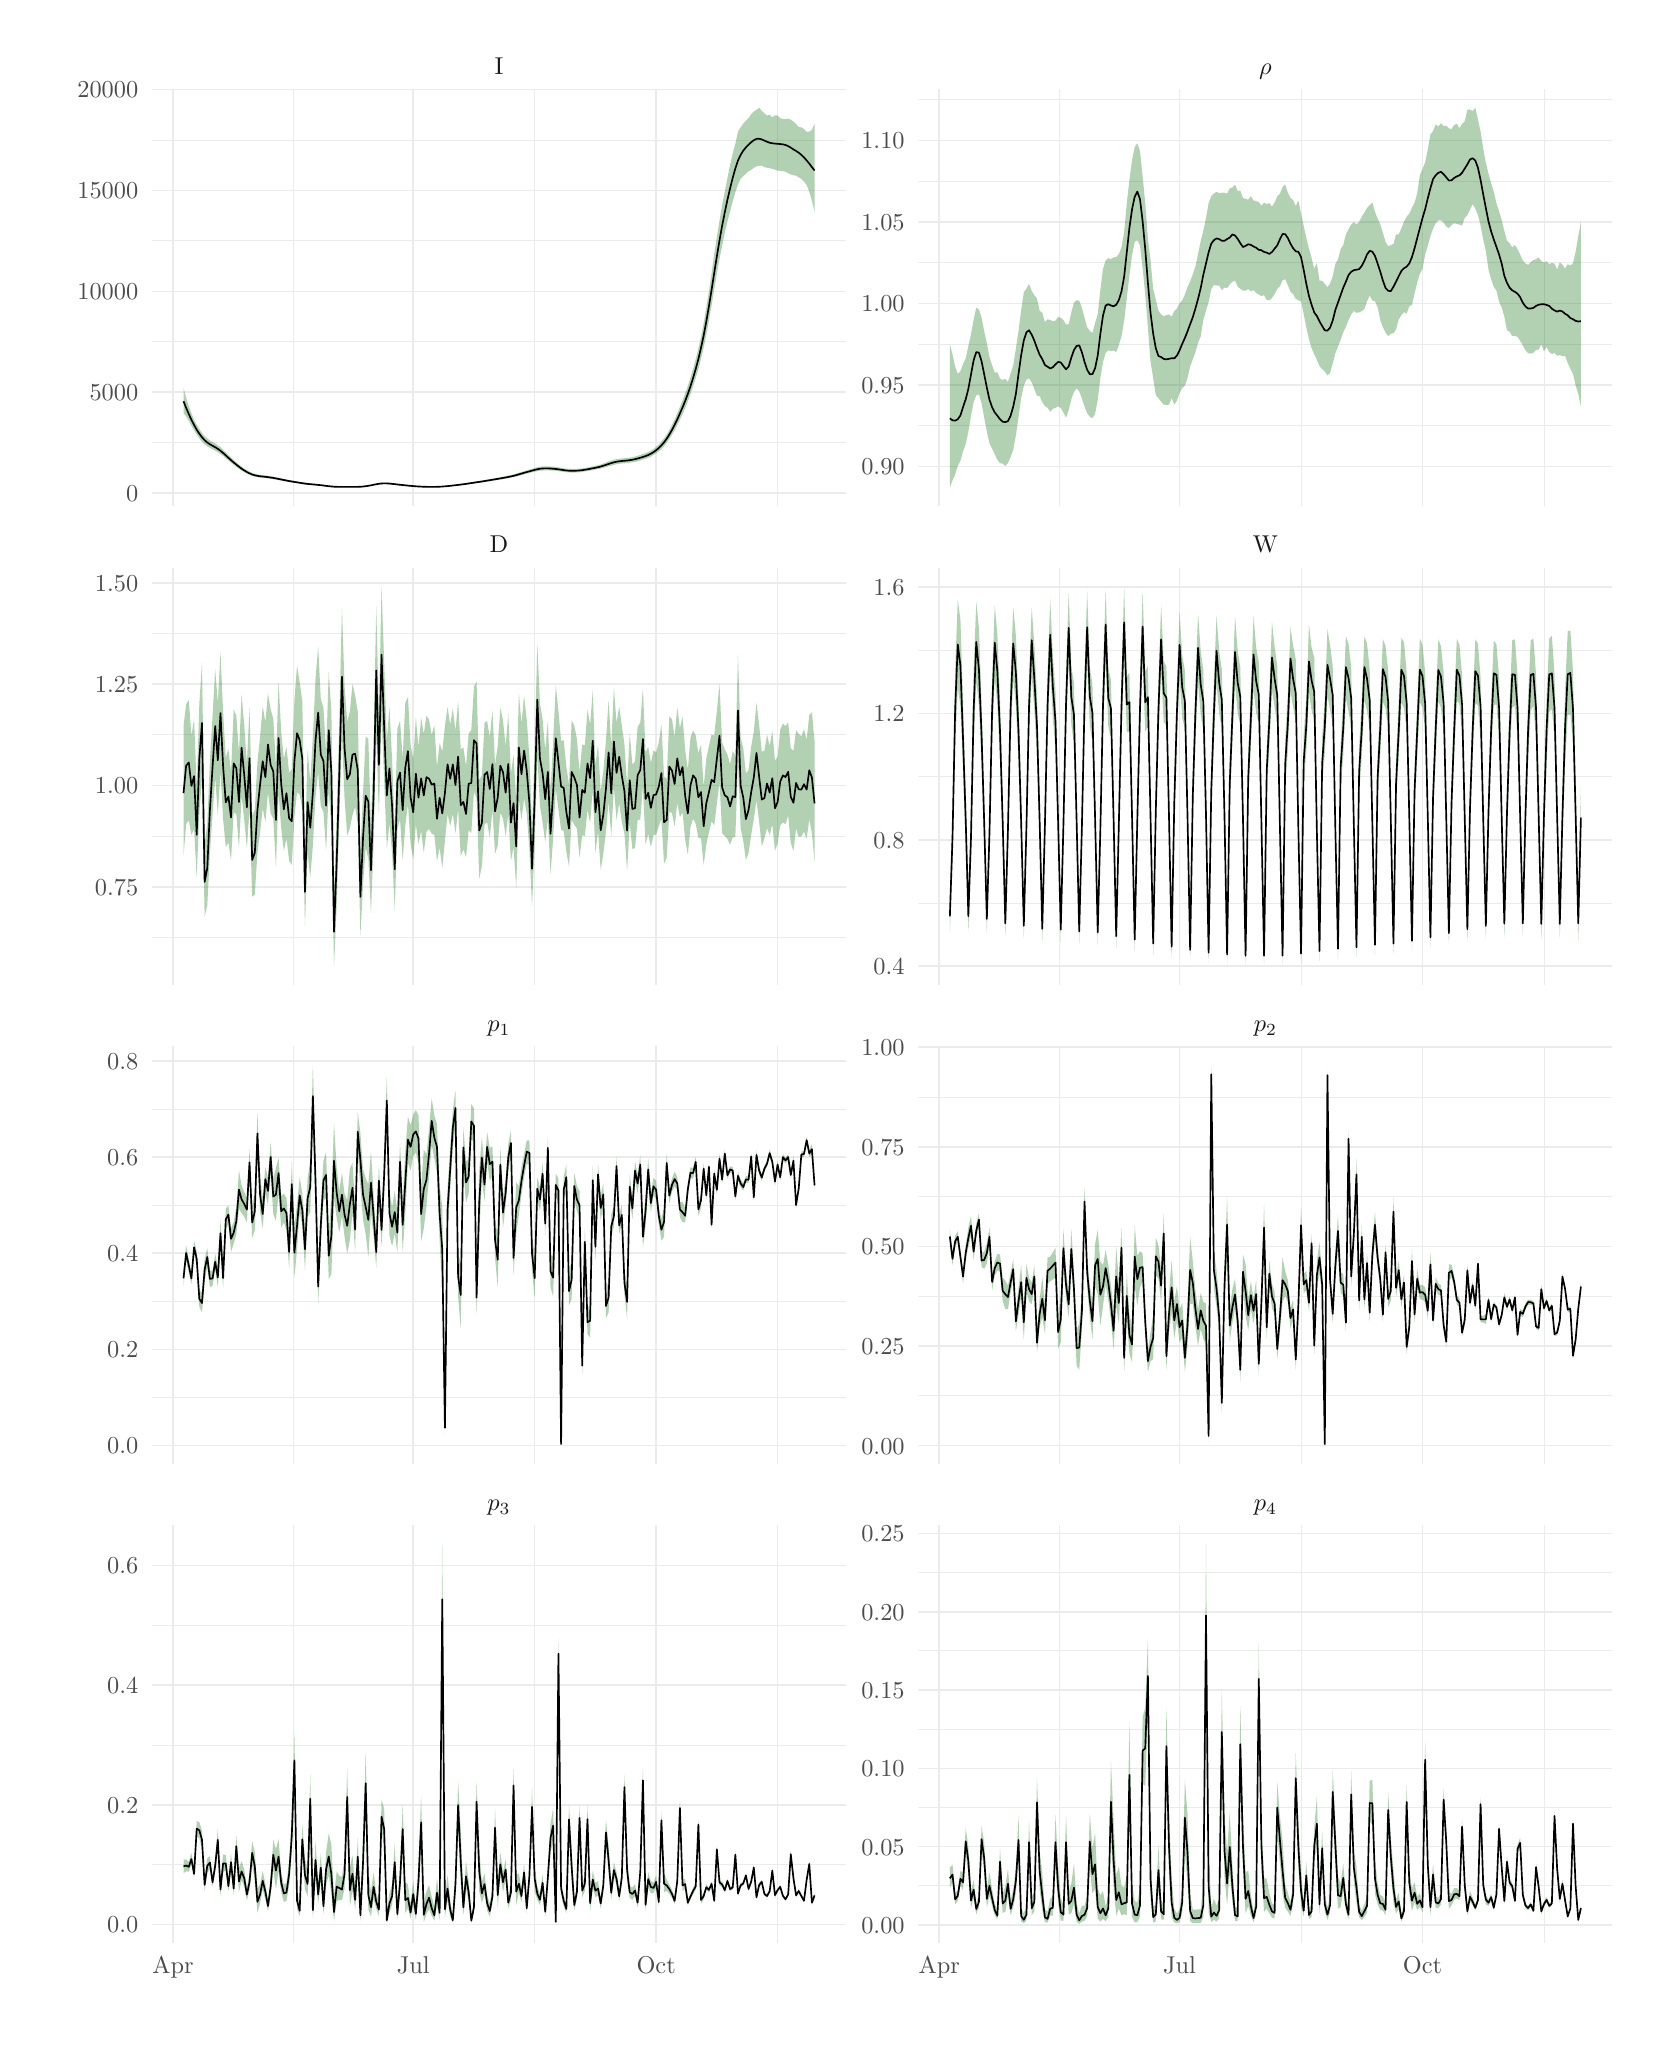
\begin{tikzpicture}[x=1pt,y=1pt]
\definecolor{fillColor}{RGB}{255,255,255}
\path[use as bounding box,fill=fillColor,fill opacity=0.00] (0,0) rectangle (578.16,722.70);
\begin{scope}
\path[clip] ( 44.91,549.70) rectangle (295.74,700.63);
\definecolor{drawColor}{gray}{0.92}

\path[draw=drawColor,line width= 0.3pt,line join=round] ( 44.91,572.69) --
	(295.74,572.69);

\path[draw=drawColor,line width= 0.3pt,line join=round] ( 44.91,609.17) --
	(295.74,609.17);

\path[draw=drawColor,line width= 0.3pt,line join=round] ( 44.91,645.65) --
	(295.74,645.65);

\path[draw=drawColor,line width= 0.3pt,line join=round] ( 44.91,682.13) --
	(295.74,682.13);

\path[draw=drawColor,line width= 0.3pt,line join=round] ( 95.91,549.70) --
	( 95.91,700.63);

\path[draw=drawColor,line width= 0.3pt,line join=round] (183.20,549.70) --
	(183.20,700.63);

\path[draw=drawColor,line width= 0.3pt,line join=round] (270.98,549.70) --
	(270.98,700.63);

\path[draw=drawColor,line width= 0.6pt,line join=round] ( 44.91,554.45) --
	(295.74,554.45);

\path[draw=drawColor,line width= 0.6pt,line join=round] ( 44.91,590.93) --
	(295.74,590.93);

\path[draw=drawColor,line width= 0.6pt,line join=round] ( 44.91,627.41) --
	(295.74,627.41);

\path[draw=drawColor,line width= 0.6pt,line join=round] ( 44.91,663.89) --
	(295.74,663.89);

\path[draw=drawColor,line width= 0.6pt,line join=round] ( 44.91,700.37) --
	(295.74,700.37);

\path[draw=drawColor,line width= 0.6pt,line join=round] ( 52.49,549.70) --
	( 52.49,700.63);

\path[draw=drawColor,line width= 0.6pt,line join=round] (139.32,549.70) --
	(139.32,700.63);

\path[draw=drawColor,line width= 0.6pt,line join=round] (227.09,549.70) --
	(227.09,700.63);
\definecolor{fillColor}{RGB}{0,100,0}

\path[fill=fillColor,fill opacity=0.30] ( 56.31,592.55) --
	( 57.26,588.96) --
	( 58.22,585.92) --
	( 59.17,583.32) --
	( 60.13,581.07) --
	( 61.08,579.25) --
	( 62.03,577.65) --
	( 62.99,576.24) --
	( 63.94,575.09) --
	( 64.90,574.27) --
	( 65.85,573.49) --
	( 66.81,572.93) --
	( 67.76,572.48) --
	( 68.71,571.83) --
	( 69.67,571.09) --
	( 70.62,570.18) --
	( 71.58,569.27) --
	( 72.53,568.28) --
	( 73.48,567.40) --
	( 74.44,566.45) --
	( 75.39,565.60) --
	( 76.35,564.81) --
	( 77.30,564.08) --
	( 78.25,563.38) --
	( 79.21,562.79) --
	( 80.16,562.25) --
	( 81.12,561.81) --
	( 82.07,561.50) --
	( 83.02,561.27) --
	( 83.98,561.11) --
	( 84.93,561.01) --
	( 85.89,560.89) --
	( 86.84,560.76) --
	( 87.80,560.61) --
	( 88.75,560.46) --
	( 89.70,560.24) --
	( 90.66,560.05) --
	( 91.61,559.83) --
	( 92.57,559.62) --
	( 93.52,559.43) --
	( 94.47,559.23) --
	( 95.43,559.06) --
	( 96.38,558.91) --
	( 97.34,558.74) --
	( 98.29,558.58) --
	( 99.24,558.42) --
	(100.20,558.24) --
	(101.15,558.13) --
	(102.11,558.04) --
	(103.06,557.92) --
	(104.01,557.83) --
	(104.97,557.73) --
	(105.92,557.61) --
	(106.88,557.48) --
	(107.83,557.37) --
	(108.79,557.24) --
	(109.74,557.13) --
	(110.69,557.05) --
	(111.65,556.99) --
	(112.60,556.97) --
	(113.56,556.96) --
	(114.51,556.96) --
	(115.46,556.96) --
	(116.42,556.96) --
	(117.37,556.96) --
	(118.33,556.97) --
	(119.28,556.99) --
	(120.23,557.02) --
	(121.19,557.11) --
	(122.14,557.22) --
	(123.10,557.38) --
	(124.05,557.56) --
	(125.00,557.77) --
	(125.96,557.99) --
	(126.91,558.16) --
	(127.87,558.29) --
	(128.82,558.31) --
	(129.78,558.29) --
	(130.73,558.24) --
	(131.68,558.15) --
	(132.64,558.04) --
	(133.59,557.91) --
	(134.55,557.80) --
	(135.50,557.68) --
	(136.45,557.57) --
	(137.41,557.45) --
	(138.36,557.34) --
	(139.32,557.26) --
	(140.27,557.18) --
	(141.22,557.10) --
	(142.18,557.05) --
	(143.13,557.00) --
	(144.09,556.97) --
	(145.04,556.96) --
	(145.99,556.95) --
	(146.95,556.95) --
	(147.90,556.98) --
	(148.86,557.02) --
	(149.81,557.08) --
	(150.77,557.17) --
	(151.72,557.26) --
	(152.67,557.37) --
	(153.63,557.47) --
	(154.58,557.59) --
	(155.54,557.72) --
	(156.49,557.84) --
	(157.44,557.99) --
	(158.40,558.13) --
	(159.35,558.27) --
	(160.31,558.44) --
	(161.26,558.59) --
	(162.21,558.74) --
	(163.17,558.92) --
	(164.12,559.08) --
	(165.08,559.24) --
	(166.03,559.37) --
	(166.98,559.54) --
	(167.94,559.71) --
	(168.89,559.89) --
	(169.85,560.08) --
	(170.80,560.25) --
	(171.76,560.45) --
	(172.71,560.65) --
	(173.66,560.84) --
	(174.62,561.06) --
	(175.57,561.30) --
	(176.53,561.60) --
	(177.48,561.86) --
	(178.43,562.14) --
	(179.39,562.39) --
	(180.34,562.70) --
	(181.30,563.00) --
	(182.25,563.27) --
	(183.20,563.58) --
	(184.16,563.85) --
	(185.11,564.00) --
	(186.07,564.13) --
	(187.02,564.18) --
	(187.97,564.15) --
	(188.93,564.11) --
	(189.88,564.05) --
	(190.84,563.96) --
	(191.79,563.81) --
	(192.75,563.65) --
	(193.70,563.48) --
	(194.65,563.32) --
	(195.61,563.28) --
	(196.56,563.21) --
	(197.52,563.20) --
	(198.47,563.24) --
	(199.42,563.32) --
	(200.38,563.44) --
	(201.33,563.59) --
	(202.29,563.78) --
	(203.24,563.96) --
	(204.19,564.18) --
	(205.15,564.38) --
	(206.10,564.57) --
	(207.06,564.83) --
	(208.01,565.19) --
	(208.96,565.57) --
	(209.92,565.97) --
	(210.87,566.23) --
	(211.83,566.55) --
	(212.78,566.77) --
	(213.74,566.92) --
	(214.69,567.02) --
	(215.64,567.11) --
	(216.60,567.26) --
	(217.55,567.31) --
	(218.51,567.49) --
	(219.46,567.72) --
	(220.41,567.99) --
	(221.37,568.28) --
	(222.32,568.65) --
	(223.28,568.95) --
	(224.23,569.36) --
	(225.18,569.86) --
	(226.14,570.42) --
	(227.09,571.14) --
	(228.05,572.08) --
	(229.00,573.13) --
	(229.95,574.26) --
	(230.91,575.67) --
	(231.86,577.29) --
	(232.82,579.17) --
	(233.77,581.16) --
	(234.73,583.35) --
	(235.68,585.62) --
	(236.63,587.99) --
	(237.59,590.56) --
	(238.54,593.20) --
	(239.50,596.31) --
	(240.45,599.45) --
	(241.40,602.94) --
	(242.36,606.78) --
	(243.31,611.02) --
	(244.27,615.96) --
	(245.22,621.51) --
	(246.17,627.45) --
	(247.13,633.89) --
	(248.08,640.90) --
	(249.04,647.06) --
	(249.99,652.97) --
	(250.94,658.61) --
	(251.90,663.44) --
	(252.85,668.40) --
	(253.81,672.98) --
	(254.76,677.21) --
	(255.72,680.76) --
	(256.67,685.12) --
	(257.62,686.62) --
	(258.58,688.04) --
	(259.53,689.08) --
	(260.49,690.04) --
	(261.44,691.42) --
	(262.39,692.38) --
	(263.35,693.00) --
	(264.30,693.77) --
	(265.26,692.62) --
	(266.21,691.77) --
	(267.16,690.96) --
	(268.12,691.18) --
	(269.07,690.31) --
	(270.03,691.04) --
	(270.98,690.94) --
	(271.93,690.01) --
	(272.89,689.67) --
	(273.84,689.61) --
	(274.80,689.86) --
	(275.75,689.39) --
	(276.71,688.78) --
	(277.66,687.88) --
	(278.61,686.74) --
	(279.57,686.69) --
	(280.52,686.05) --
	(281.48,685.07) --
	(282.43,685.10) --
	(283.38,685.80) --
	(284.34,688.02) --
	(284.34,656.02) --
	(283.38,660.18) --
	(282.43,663.37) --
	(281.48,665.86) --
	(280.52,667.07) --
	(279.57,668.08) --
	(278.61,668.57) --
	(277.66,669.21) --
	(276.71,669.35) --
	(275.75,669.67) --
	(274.80,670.10) --
	(273.84,670.61) --
	(272.89,670.86) --
	(271.93,670.98) --
	(270.98,671.01) --
	(270.03,671.39) --
	(269.07,671.63) --
	(268.12,671.93) --
	(267.16,672.09) --
	(266.21,672.29) --
	(265.26,672.89) --
	(264.30,672.71) --
	(263.35,672.58) --
	(262.39,672.07) --
	(261.44,671.29) --
	(260.49,670.79) --
	(259.53,669.94) --
	(258.58,669.03) --
	(257.62,668.09) --
	(256.67,665.96) --
	(255.72,663.23) --
	(254.76,659.89) --
	(253.81,656.24) --
	(252.85,652.66) --
	(251.90,648.64) --
	(250.94,643.84) --
	(249.99,639.18) --
	(249.04,633.86) --
	(248.08,628.03) --
	(247.13,622.34) --
	(246.17,616.81) --
	(245.22,611.68) --
	(244.27,607.15) --
	(243.31,602.92) --
	(242.36,599.34) --
	(241.40,596.14) --
	(240.45,593.06) --
	(239.50,590.23) --
	(238.54,587.63) --
	(237.59,585.18) --
	(236.63,583.03) --
	(235.68,581.02) --
	(234.73,579.13) --
	(233.77,577.21) --
	(232.82,575.61) --
	(231.86,574.07) --
	(230.91,572.74) --
	(229.95,571.45) --
	(229.00,570.44) --
	(228.05,569.59) --
	(227.09,568.87) --
	(226.14,568.29) --
	(225.18,567.70) --
	(224.23,567.25) --
	(223.28,566.92) --
	(222.32,566.60) --
	(221.37,566.27) --
	(220.41,565.99) --
	(219.46,565.79) --
	(218.51,565.67) --
	(217.55,565.53) --
	(216.60,565.38) --
	(215.64,565.28) --
	(214.69,565.20) --
	(213.74,565.09) --
	(212.78,564.94) --
	(211.83,564.71) --
	(210.87,564.42) --
	(209.92,564.22) --
	(208.96,563.92) --
	(208.01,563.63) --
	(207.06,563.36) --
	(206.10,563.19) --
	(205.15,563.02) --
	(204.19,562.83) --
	(203.24,562.63) --
	(202.29,562.47) --
	(201.33,562.33) --
	(200.38,562.15) --
	(199.42,562.04) --
	(198.47,561.97) --
	(197.52,561.94) --
	(196.56,561.92) --
	(195.61,561.97) --
	(194.65,562.05) --
	(193.70,562.18) --
	(192.75,562.31) --
	(191.79,562.45) --
	(190.84,562.57) --
	(189.88,562.66) --
	(188.93,562.67) --
	(187.97,562.73) --
	(187.02,562.72) --
	(186.07,562.70) --
	(185.11,562.59) --
	(184.16,562.43) --
	(183.20,562.24) --
	(182.25,562.01) --
	(181.30,561.77) --
	(180.34,561.54) --
	(179.39,561.30) --
	(178.43,561.02) --
	(177.48,560.75) --
	(176.53,560.50) --
	(175.57,560.26) --
	(174.62,560.07) --
	(173.66,559.87) --
	(172.71,559.72) --
	(171.76,559.56) --
	(170.80,559.41) --
	(169.85,559.25) --
	(168.89,559.10) --
	(167.94,558.94) --
	(166.98,558.79) --
	(166.03,558.65) --
	(165.08,558.50) --
	(164.12,558.35) --
	(163.17,558.22) --
	(162.21,558.11) --
	(161.26,557.98) --
	(160.31,557.84) --
	(159.35,557.70) --
	(158.40,557.56) --
	(157.44,557.45) --
	(156.49,557.34) --
	(155.54,557.22) --
	(154.58,557.11) --
	(153.63,557.02) --
	(152.67,556.93) --
	(151.72,556.84) --
	(150.77,556.75) --
	(149.81,556.69) --
	(148.86,556.64) --
	(147.90,556.58) --
	(146.95,556.56) --
	(145.99,556.56) --
	(145.04,556.57) --
	(144.09,556.58) --
	(143.13,556.62) --
	(142.18,556.67) --
	(141.22,556.71) --
	(140.27,556.76) --
	(139.32,556.84) --
	(138.36,556.92) --
	(137.41,557.00) --
	(136.45,557.10) --
	(135.50,557.18) --
	(134.55,557.27) --
	(133.59,557.38) --
	(132.64,557.47) --
	(131.68,557.58) --
	(130.73,557.67) --
	(129.78,557.73) --
	(128.82,557.76) --
	(127.87,557.72) --
	(126.91,557.61) --
	(125.96,557.46) --
	(125.00,557.28) --
	(124.05,557.09) --
	(123.10,556.91) --
	(122.14,556.78) --
	(121.19,556.69) --
	(120.23,556.63) --
	(119.28,556.59) --
	(118.33,556.58) --
	(117.37,556.57) --
	(116.42,556.57) --
	(115.46,556.57) --
	(114.51,556.57) --
	(113.56,556.57) --
	(112.60,556.57) --
	(111.65,556.58) --
	(110.69,556.62) --
	(109.74,556.70) --
	(108.79,556.79) --
	(107.83,556.89) --
	(106.88,557.02) --
	(105.92,557.14) --
	(104.97,557.24) --
	(104.01,557.32) --
	(103.06,557.38) --
	(102.11,557.46) --
	(101.15,557.54) --
	(100.20,557.62) --
	( 99.24,557.76) --
	( 98.29,557.93) --
	( 97.34,558.09) --
	( 96.38,558.24) --
	( 95.43,558.36) --
	( 94.47,558.50) --
	( 93.52,558.68) --
	( 92.57,558.85) --
	( 91.61,559.01) --
	( 90.66,559.21) --
	( 89.70,559.38) --
	( 88.75,559.53) --
	( 87.80,559.67) --
	( 86.84,559.80) --
	( 85.89,559.93) --
	( 84.93,560.01) --
	( 83.98,560.13) --
	( 83.02,560.27) --
	( 82.07,560.45) --
	( 81.12,560.73) --
	( 80.16,561.12) --
	( 79.21,561.57) --
	( 78.25,562.08) --
	( 77.30,562.67) --
	( 76.35,563.33) --
	( 75.39,564.03) --
	( 74.44,564.77) --
	( 73.48,565.52) --
	( 72.53,566.32) --
	( 71.58,567.11) --
	( 70.62,567.96) --
	( 69.67,568.64) --
	( 68.71,569.26) --
	( 67.76,569.86) --
	( 66.81,570.36) --
	( 65.85,570.85) --
	( 64.90,571.37) --
	( 63.94,572.16) --
	( 62.99,573.09) --
	( 62.03,574.26) --
	( 61.08,575.68) --
	( 60.13,577.23) --
	( 59.17,578.89) --
	( 58.22,580.61) --
	( 57.26,582.20) --
	( 56.31,583.46) --
	cycle;

\path[] ( 56.31,592.55) --
	( 57.26,588.96) --
	( 58.22,585.92) --
	( 59.17,583.32) --
	( 60.13,581.07) --
	( 61.08,579.25) --
	( 62.03,577.65) --
	( 62.99,576.24) --
	( 63.94,575.09) --
	( 64.90,574.27) --
	( 65.85,573.49) --
	( 66.81,572.93) --
	( 67.76,572.48) --
	( 68.71,571.83) --
	( 69.67,571.09) --
	( 70.62,570.18) --
	( 71.58,569.27) --
	( 72.53,568.28) --
	( 73.48,567.40) --
	( 74.44,566.45) --
	( 75.39,565.60) --
	( 76.35,564.81) --
	( 77.30,564.08) --
	( 78.25,563.38) --
	( 79.21,562.79) --
	( 80.16,562.25) --
	( 81.12,561.81) --
	( 82.07,561.50) --
	( 83.02,561.27) --
	( 83.98,561.11) --
	( 84.93,561.01) --
	( 85.89,560.89) --
	( 86.84,560.76) --
	( 87.80,560.61) --
	( 88.75,560.46) --
	( 89.70,560.24) --
	( 90.66,560.05) --
	( 91.61,559.83) --
	( 92.57,559.62) --
	( 93.52,559.43) --
	( 94.47,559.23) --
	( 95.43,559.06) --
	( 96.38,558.91) --
	( 97.34,558.74) --
	( 98.29,558.58) --
	( 99.24,558.42) --
	(100.20,558.24) --
	(101.15,558.13) --
	(102.11,558.04) --
	(103.06,557.92) --
	(104.01,557.83) --
	(104.97,557.73) --
	(105.92,557.61) --
	(106.88,557.48) --
	(107.83,557.37) --
	(108.79,557.24) --
	(109.74,557.13) --
	(110.69,557.05) --
	(111.65,556.99) --
	(112.60,556.97) --
	(113.56,556.96) --
	(114.51,556.96) --
	(115.46,556.96) --
	(116.42,556.96) --
	(117.37,556.96) --
	(118.33,556.97) --
	(119.28,556.99) --
	(120.23,557.02) --
	(121.19,557.11) --
	(122.14,557.22) --
	(123.10,557.38) --
	(124.05,557.56) --
	(125.00,557.77) --
	(125.96,557.99) --
	(126.91,558.16) --
	(127.87,558.29) --
	(128.82,558.31) --
	(129.78,558.29) --
	(130.73,558.24) --
	(131.68,558.15) --
	(132.64,558.04) --
	(133.59,557.91) --
	(134.55,557.80) --
	(135.50,557.68) --
	(136.45,557.57) --
	(137.41,557.45) --
	(138.36,557.34) --
	(139.32,557.26) --
	(140.27,557.18) --
	(141.22,557.10) --
	(142.18,557.05) --
	(143.13,557.00) --
	(144.09,556.97) --
	(145.04,556.96) --
	(145.99,556.95) --
	(146.95,556.95) --
	(147.90,556.98) --
	(148.86,557.02) --
	(149.81,557.08) --
	(150.77,557.17) --
	(151.72,557.26) --
	(152.67,557.37) --
	(153.63,557.47) --
	(154.58,557.59) --
	(155.54,557.72) --
	(156.49,557.84) --
	(157.44,557.99) --
	(158.40,558.13) --
	(159.35,558.27) --
	(160.31,558.44) --
	(161.26,558.59) --
	(162.21,558.74) --
	(163.17,558.92) --
	(164.12,559.08) --
	(165.08,559.24) --
	(166.03,559.37) --
	(166.98,559.54) --
	(167.94,559.71) --
	(168.89,559.89) --
	(169.85,560.08) --
	(170.80,560.25) --
	(171.76,560.45) --
	(172.71,560.65) --
	(173.66,560.84) --
	(174.62,561.06) --
	(175.57,561.30) --
	(176.53,561.60) --
	(177.48,561.86) --
	(178.43,562.14) --
	(179.39,562.39) --
	(180.34,562.70) --
	(181.30,563.00) --
	(182.25,563.27) --
	(183.20,563.58) --
	(184.16,563.85) --
	(185.11,564.00) --
	(186.07,564.13) --
	(187.02,564.18) --
	(187.97,564.15) --
	(188.93,564.11) --
	(189.88,564.05) --
	(190.84,563.96) --
	(191.79,563.81) --
	(192.75,563.65) --
	(193.70,563.48) --
	(194.65,563.32) --
	(195.61,563.28) --
	(196.56,563.21) --
	(197.52,563.20) --
	(198.47,563.24) --
	(199.42,563.32) --
	(200.38,563.44) --
	(201.33,563.59) --
	(202.29,563.78) --
	(203.24,563.96) --
	(204.19,564.18) --
	(205.15,564.38) --
	(206.10,564.57) --
	(207.06,564.83) --
	(208.01,565.19) --
	(208.96,565.57) --
	(209.92,565.97) --
	(210.87,566.23) --
	(211.83,566.55) --
	(212.78,566.77) --
	(213.74,566.92) --
	(214.69,567.02) --
	(215.64,567.11) --
	(216.60,567.26) --
	(217.55,567.31) --
	(218.51,567.49) --
	(219.46,567.72) --
	(220.41,567.99) --
	(221.37,568.28) --
	(222.32,568.65) --
	(223.28,568.95) --
	(224.23,569.36) --
	(225.18,569.86) --
	(226.14,570.42) --
	(227.09,571.14) --
	(228.05,572.08) --
	(229.00,573.13) --
	(229.95,574.26) --
	(230.91,575.67) --
	(231.86,577.29) --
	(232.82,579.17) --
	(233.77,581.16) --
	(234.73,583.35) --
	(235.68,585.62) --
	(236.63,587.99) --
	(237.59,590.56) --
	(238.54,593.20) --
	(239.50,596.31) --
	(240.45,599.45) --
	(241.40,602.94) --
	(242.36,606.78) --
	(243.31,611.02) --
	(244.27,615.96) --
	(245.22,621.51) --
	(246.17,627.45) --
	(247.13,633.89) --
	(248.08,640.90) --
	(249.04,647.06) --
	(249.99,652.97) --
	(250.94,658.61) --
	(251.90,663.44) --
	(252.85,668.40) --
	(253.81,672.98) --
	(254.76,677.21) --
	(255.72,680.76) --
	(256.67,685.12) --
	(257.62,686.62) --
	(258.58,688.04) --
	(259.53,689.08) --
	(260.49,690.04) --
	(261.44,691.42) --
	(262.39,692.38) --
	(263.35,693.00) --
	(264.30,693.77) --
	(265.26,692.62) --
	(266.21,691.77) --
	(267.16,690.96) --
	(268.12,691.18) --
	(269.07,690.31) --
	(270.03,691.04) --
	(270.98,690.94) --
	(271.93,690.01) --
	(272.89,689.67) --
	(273.84,689.61) --
	(274.80,689.86) --
	(275.75,689.39) --
	(276.71,688.78) --
	(277.66,687.88) --
	(278.61,686.74) --
	(279.57,686.69) --
	(280.52,686.05) --
	(281.48,685.07) --
	(282.43,685.10) --
	(283.38,685.80) --
	(284.34,688.02);

\path[] (284.34,656.02) --
	(283.38,660.18) --
	(282.43,663.37) --
	(281.48,665.86) --
	(280.52,667.07) --
	(279.57,668.08) --
	(278.61,668.57) --
	(277.66,669.21) --
	(276.71,669.35) --
	(275.75,669.67) --
	(274.80,670.10) --
	(273.84,670.61) --
	(272.89,670.86) --
	(271.93,670.98) --
	(270.98,671.01) --
	(270.03,671.39) --
	(269.07,671.63) --
	(268.12,671.93) --
	(267.16,672.09) --
	(266.21,672.29) --
	(265.26,672.89) --
	(264.30,672.71) --
	(263.35,672.58) --
	(262.39,672.07) --
	(261.44,671.29) --
	(260.49,670.79) --
	(259.53,669.94) --
	(258.58,669.03) --
	(257.62,668.09) --
	(256.67,665.96) --
	(255.72,663.23) --
	(254.76,659.89) --
	(253.81,656.24) --
	(252.85,652.66) --
	(251.90,648.64) --
	(250.94,643.84) --
	(249.99,639.18) --
	(249.04,633.86) --
	(248.08,628.03) --
	(247.13,622.34) --
	(246.17,616.81) --
	(245.22,611.68) --
	(244.27,607.15) --
	(243.31,602.92) --
	(242.36,599.34) --
	(241.40,596.14) --
	(240.45,593.06) --
	(239.50,590.23) --
	(238.54,587.63) --
	(237.59,585.18) --
	(236.63,583.03) --
	(235.68,581.02) --
	(234.73,579.13) --
	(233.77,577.21) --
	(232.82,575.61) --
	(231.86,574.07) --
	(230.91,572.74) --
	(229.95,571.45) --
	(229.00,570.44) --
	(228.05,569.59) --
	(227.09,568.87) --
	(226.14,568.29) --
	(225.18,567.70) --
	(224.23,567.25) --
	(223.28,566.92) --
	(222.32,566.60) --
	(221.37,566.27) --
	(220.41,565.99) --
	(219.46,565.79) --
	(218.51,565.67) --
	(217.55,565.53) --
	(216.60,565.38) --
	(215.64,565.28) --
	(214.69,565.20) --
	(213.74,565.09) --
	(212.78,564.94) --
	(211.83,564.71) --
	(210.87,564.42) --
	(209.92,564.22) --
	(208.96,563.92) --
	(208.01,563.63) --
	(207.06,563.36) --
	(206.10,563.19) --
	(205.15,563.02) --
	(204.19,562.83) --
	(203.24,562.63) --
	(202.29,562.47) --
	(201.33,562.33) --
	(200.38,562.15) --
	(199.42,562.04) --
	(198.47,561.97) --
	(197.52,561.94) --
	(196.56,561.92) --
	(195.61,561.97) --
	(194.65,562.05) --
	(193.70,562.18) --
	(192.75,562.31) --
	(191.79,562.45) --
	(190.84,562.57) --
	(189.88,562.66) --
	(188.93,562.67) --
	(187.97,562.73) --
	(187.02,562.72) --
	(186.07,562.70) --
	(185.11,562.59) --
	(184.16,562.43) --
	(183.20,562.24) --
	(182.25,562.01) --
	(181.30,561.77) --
	(180.34,561.54) --
	(179.39,561.30) --
	(178.43,561.02) --
	(177.48,560.75) --
	(176.53,560.50) --
	(175.57,560.26) --
	(174.62,560.07) --
	(173.66,559.87) --
	(172.71,559.72) --
	(171.76,559.56) --
	(170.80,559.41) --
	(169.85,559.25) --
	(168.89,559.10) --
	(167.94,558.94) --
	(166.98,558.79) --
	(166.03,558.65) --
	(165.08,558.50) --
	(164.12,558.35) --
	(163.17,558.22) --
	(162.21,558.11) --
	(161.26,557.98) --
	(160.31,557.84) --
	(159.35,557.70) --
	(158.40,557.56) --
	(157.44,557.45) --
	(156.49,557.34) --
	(155.54,557.22) --
	(154.58,557.11) --
	(153.63,557.02) --
	(152.67,556.93) --
	(151.72,556.84) --
	(150.77,556.75) --
	(149.81,556.69) --
	(148.86,556.64) --
	(147.90,556.58) --
	(146.95,556.56) --
	(145.99,556.56) --
	(145.04,556.57) --
	(144.09,556.58) --
	(143.13,556.62) --
	(142.18,556.67) --
	(141.22,556.71) --
	(140.27,556.76) --
	(139.32,556.84) --
	(138.36,556.92) --
	(137.41,557.00) --
	(136.45,557.10) --
	(135.50,557.18) --
	(134.55,557.27) --
	(133.59,557.38) --
	(132.64,557.47) --
	(131.68,557.58) --
	(130.73,557.67) --
	(129.78,557.73) --
	(128.82,557.76) --
	(127.87,557.72) --
	(126.91,557.61) --
	(125.96,557.46) --
	(125.00,557.28) --
	(124.05,557.09) --
	(123.10,556.91) --
	(122.14,556.78) --
	(121.19,556.69) --
	(120.23,556.63) --
	(119.28,556.59) --
	(118.33,556.58) --
	(117.37,556.57) --
	(116.42,556.57) --
	(115.46,556.57) --
	(114.51,556.57) --
	(113.56,556.57) --
	(112.60,556.57) --
	(111.65,556.58) --
	(110.69,556.62) --
	(109.74,556.70) --
	(108.79,556.79) --
	(107.83,556.89) --
	(106.88,557.02) --
	(105.92,557.14) --
	(104.97,557.24) --
	(104.01,557.32) --
	(103.06,557.38) --
	(102.11,557.46) --
	(101.15,557.54) --
	(100.20,557.62) --
	( 99.24,557.76) --
	( 98.29,557.93) --
	( 97.34,558.09) --
	( 96.38,558.24) --
	( 95.43,558.36) --
	( 94.47,558.50) --
	( 93.52,558.68) --
	( 92.57,558.85) --
	( 91.61,559.01) --
	( 90.66,559.21) --
	( 89.70,559.38) --
	( 88.75,559.53) --
	( 87.80,559.67) --
	( 86.84,559.80) --
	( 85.89,559.93) --
	( 84.93,560.01) --
	( 83.98,560.13) --
	( 83.02,560.27) --
	( 82.07,560.45) --
	( 81.12,560.73) --
	( 80.16,561.12) --
	( 79.21,561.57) --
	( 78.25,562.08) --
	( 77.30,562.67) --
	( 76.35,563.33) --
	( 75.39,564.03) --
	( 74.44,564.77) --
	( 73.48,565.52) --
	( 72.53,566.32) --
	( 71.58,567.11) --
	( 70.62,567.96) --
	( 69.67,568.64) --
	( 68.71,569.26) --
	( 67.76,569.86) --
	( 66.81,570.36) --
	( 65.85,570.85) --
	( 64.90,571.37) --
	( 63.94,572.16) --
	( 62.99,573.09) --
	( 62.03,574.26) --
	( 61.08,575.68) --
	( 60.13,577.23) --
	( 59.17,578.89) --
	( 58.22,580.61) --
	( 57.26,582.20) --
	( 56.31,583.46);
\definecolor{drawColor}{RGB}{0,0,0}

\path[draw=drawColor,line width= 0.6pt,line join=round] ( 56.31,587.70) --
	( 57.26,585.32) --
	( 58.22,583.08) --
	( 59.17,581.01) --
	( 60.13,579.12) --
	( 61.08,577.42) --
	( 62.03,575.96) --
	( 62.99,574.69) --
	( 63.94,573.63) --
	( 64.90,572.79) --
	( 65.85,572.15) --
	( 66.81,571.61) --
	( 67.76,571.09) --
	( 68.71,570.50) --
	( 69.67,569.80) --
	( 70.62,569.01) --
	( 71.58,568.15) --
	( 72.53,567.27) --
	( 73.48,566.41) --
	( 74.44,565.59) --
	( 75.39,564.80) --
	( 76.35,564.04) --
	( 77.30,563.34) --
	( 78.25,562.70) --
	( 79.21,562.13) --
	( 80.16,561.65) --
	( 81.12,561.24) --
	( 82.07,560.95) --
	( 83.02,560.74) --
	( 83.98,560.60) --
	( 84.93,560.49) --
	( 85.89,560.39) --
	( 86.84,560.28) --
	( 87.80,560.14) --
	( 88.75,559.99) --
	( 89.70,559.81) --
	( 90.66,559.63) --
	( 91.61,559.43) --
	( 92.57,559.24) --
	( 93.52,559.05) --
	( 94.47,558.86) --
	( 95.43,558.70) --
	( 96.38,558.55) --
	( 97.34,558.40) --
	( 98.29,558.25) --
	( 99.24,558.09) --
	(100.20,557.95) --
	(101.15,557.83) --
	(102.11,557.74) --
	(103.06,557.65) --
	(104.01,557.57) --
	(104.97,557.47) --
	(105.92,557.37) --
	(106.88,557.25) --
	(107.83,557.13) --
	(108.79,557.01) --
	(109.74,556.91) --
	(110.69,556.83) --
	(111.65,556.78) --
	(112.60,556.77) --
	(113.56,556.76) --
	(114.51,556.76) --
	(115.46,556.76) --
	(116.42,556.75) --
	(117.37,556.75) --
	(118.33,556.76) --
	(119.28,556.77) --
	(120.23,556.81) --
	(121.19,556.88) --
	(122.14,557.00) --
	(123.10,557.14) --
	(124.05,557.32) --
	(125.00,557.52) --
	(125.96,557.71) --
	(126.91,557.88) --
	(127.87,557.99) --
	(128.82,558.03) --
	(129.78,558.01) --
	(130.73,557.95) --
	(131.68,557.85) --
	(132.64,557.74) --
	(133.59,557.63) --
	(134.55,557.52) --
	(135.50,557.42) --
	(136.45,557.32) --
	(137.41,557.22) --
	(138.36,557.13) --
	(139.32,557.04) --
	(140.27,556.96) --
	(141.22,556.90) --
	(142.18,556.85) --
	(143.13,556.81) --
	(144.09,556.78) --
	(145.04,556.76) --
	(145.99,556.75) --
	(146.95,556.76) --
	(147.90,556.78) --
	(148.86,556.82) --
	(149.81,556.88) --
	(150.77,556.95) --
	(151.72,557.04) --
	(152.67,557.14) --
	(153.63,557.25) --
	(154.58,557.36) --
	(155.54,557.47) --
	(156.49,557.59) --
	(157.44,557.71) --
	(158.40,557.84) --
	(159.35,557.99) --
	(160.31,558.14) --
	(161.26,558.28) --
	(162.21,558.42) --
	(163.17,558.56) --
	(164.12,558.70) --
	(165.08,558.86) --
	(166.03,559.02) --
	(166.98,559.17) --
	(167.94,559.34) --
	(168.89,559.50) --
	(169.85,559.66) --
	(170.80,559.82) --
	(171.76,559.99) --
	(172.71,560.16) --
	(173.66,560.34) --
	(174.62,560.53) --
	(175.57,560.75) --
	(176.53,561.00) --
	(177.48,561.28) --
	(178.43,561.57) --
	(179.39,561.85) --
	(180.34,562.12) --
	(181.30,562.38) --
	(182.25,562.63) --
	(183.20,562.89) --
	(184.16,563.13) --
	(185.11,563.31) --
	(186.07,563.41) --
	(187.02,563.45) --
	(187.97,563.45) --
	(188.93,563.39) --
	(189.88,563.32) --
	(190.84,563.23) --
	(191.79,563.10) --
	(192.75,562.96) --
	(193.70,562.82) --
	(194.65,562.69) --
	(195.61,562.60) --
	(196.56,562.57) --
	(197.52,562.57) --
	(198.47,562.62) --
	(199.42,562.69) --
	(200.38,562.80) --
	(201.33,562.95) --
	(202.29,563.11) --
	(203.24,563.29) --
	(204.19,563.47) --
	(205.15,563.66) --
	(206.10,563.87) --
	(207.06,564.11) --
	(208.01,564.41) --
	(208.96,564.73) --
	(209.92,565.05) --
	(210.87,565.36) --
	(211.83,565.63) --
	(212.78,565.84) --
	(213.74,566.00) --
	(214.69,566.11) --
	(215.64,566.20) --
	(216.60,566.29) --
	(217.55,566.41) --
	(218.51,566.56) --
	(219.46,566.77) --
	(220.41,567.01) --
	(221.37,567.28) --
	(222.32,567.57) --
	(223.28,567.89) --
	(224.23,568.27) --
	(225.18,568.73) --
	(226.14,569.30) --
	(227.09,569.99) --
	(228.05,570.80) --
	(229.00,571.75) --
	(229.95,572.86) --
	(230.91,574.16) --
	(231.86,575.66) --
	(232.82,577.33) --
	(233.77,579.16) --
	(234.73,581.15) --
	(235.68,583.26) --
	(236.63,585.49) --
	(237.59,587.83) --
	(238.54,590.35) --
	(239.50,593.11) --
	(240.45,596.12) --
	(241.40,599.38) --
	(242.36,602.98) --
	(243.31,606.99) --
	(244.27,611.47) --
	(245.22,616.51) --
	(246.17,622.03) --
	(247.13,627.95) --
	(248.08,634.06) --
	(249.04,640.08) --
	(249.99,645.80) --
	(250.94,651.14) --
	(251.90,655.98) --
	(252.85,660.46) --
	(253.81,664.61) --
	(254.76,668.42) --
	(255.72,671.84) --
	(256.67,674.69) --
	(257.62,676.72) --
	(258.58,678.25) --
	(259.53,679.43) --
	(260.49,680.42) --
	(261.44,681.30) --
	(262.39,682.04) --
	(263.35,682.52) --
	(264.30,682.56) --
	(265.26,682.31) --
	(266.21,681.89) --
	(267.16,681.48) --
	(268.12,681.11) --
	(269.07,680.91) --
	(270.03,680.80) --
	(270.98,680.72) --
	(271.93,680.65) --
	(272.89,680.52) --
	(273.84,680.31) --
	(274.80,679.89) --
	(275.75,679.34) --
	(276.71,678.70) --
	(277.66,678.14) --
	(278.61,677.51) --
	(279.57,676.72) --
	(280.52,675.82) --
	(281.48,674.72) --
	(282.43,673.56) --
	(283.38,672.31) --
	(284.34,671.08);
\end{scope}
\begin{scope}
\path[clip] ( 44.91,376.69) rectangle (295.74,527.62);
\definecolor{drawColor}{gray}{0.92}

\path[draw=drawColor,line width= 0.3pt,line join=round] ( 44.91,393.97) --
	(295.74,393.97);

\path[draw=drawColor,line width= 0.3pt,line join=round] ( 44.91,430.55) --
	(295.74,430.55);

\path[draw=drawColor,line width= 0.3pt,line join=round] ( 44.91,467.14) --
	(295.74,467.14);

\path[draw=drawColor,line width= 0.3pt,line join=round] ( 44.91,503.72) --
	(295.74,503.72);

\path[draw=drawColor,line width= 0.3pt,line join=round] ( 95.91,376.69) --
	( 95.91,527.62);

\path[draw=drawColor,line width= 0.3pt,line join=round] (183.20,376.69) --
	(183.20,527.62);

\path[draw=drawColor,line width= 0.3pt,line join=round] (270.98,376.69) --
	(270.98,527.62);

\path[draw=drawColor,line width= 0.6pt,line join=round] ( 44.91,412.26) --
	(295.74,412.26);

\path[draw=drawColor,line width= 0.6pt,line join=round] ( 44.91,448.84) --
	(295.74,448.84);

\path[draw=drawColor,line width= 0.6pt,line join=round] ( 44.91,485.43) --
	(295.74,485.43);

\path[draw=drawColor,line width= 0.6pt,line join=round] ( 44.91,522.01) --
	(295.74,522.01);

\path[draw=drawColor,line width= 0.6pt,line join=round] ( 52.49,376.69) --
	( 52.49,527.62);

\path[draw=drawColor,line width= 0.6pt,line join=round] (139.32,376.69) --
	(139.32,527.62);

\path[draw=drawColor,line width= 0.6pt,line join=round] (227.09,376.69) --
	(227.09,527.62);
\definecolor{fillColor}{RGB}{0,100,0}

\path[fill=fillColor,fill opacity=0.30] ( 56.31,470.36) --
	( 57.26,478.27) --
	( 58.22,479.73) --
	( 59.17,466.72) --
	( 60.13,473.03) --
	( 61.08,447.97) --
	( 62.03,478.40) --
	( 62.99,493.15) --
	( 63.94,428.25) --
	( 64.90,434.67) --
	( 65.85,457.80) --
	( 66.81,474.14) --
	( 67.76,490.91) --
	( 68.71,478.61) --
	( 69.67,497.10) --
	( 70.62,475.47) --
	( 71.58,458.91) --
	( 72.53,462.05) --
	( 73.48,453.81) --
	( 74.44,476.32) --
	( 75.39,474.17) --
	( 76.35,460.75) --
	( 77.30,481.79) --
	( 78.25,470.71) --
	( 79.21,456.81) --
	( 80.16,477.10) --
	( 81.12,437.91) --
	( 82.07,440.05) --
	( 83.02,457.24) --
	( 83.98,466.62) --
	( 84.93,477.49) --
	( 85.89,471.75) --
	( 86.84,482.25) --
	( 87.80,476.36) --
	( 88.75,473.02) --
	( 89.70,456.21) --
	( 90.66,486.55) --
	( 91.61,468.12) --
	( 92.57,458.51) --
	( 93.52,462.84) --
	( 94.47,453.42) --
	( 95.43,454.74) --
	( 96.38,479.88) --
	( 97.34,492.10) --
	( 98.29,486.10) --
	( 99.24,479.33) --
	(100.20,425.56) --
	(101.15,461.80) --
	(102.11,450.30) --
	(103.06,466.77) --
	(104.01,487.31) --
	(104.97,499.15) --
	(105.92,480.17) --
	(106.88,476.82) --
	(107.83,460.66) --
	(108.79,489.81) --
	(109.74,475.68) --
	(110.69,410.13) --
	(111.65,437.10) --
	(112.60,472.39) --
	(113.56,513.22) --
	(114.51,484.81) --
	(115.46,471.82) --
	(116.42,475.55) --
	(117.37,485.53) --
	(118.33,481.37) --
	(119.28,475.47) --
	(120.23,423.98) --
	(121.19,446.35) --
	(122.14,466.53) --
	(123.10,465.67) --
	(124.05,434.30) --
	(125.00,464.49) --
	(125.96,513.71) --
	(126.91,474.93) --
	(127.87,520.76) --
	(128.82,493.18) --
	(129.78,465.37) --
	(130.73,477.28) --
	(131.68,458.37) --
	(132.64,433.23) --
	(133.59,469.45) --
	(134.55,472.29) --
	(135.50,458.72) --
	(136.45,478.77) --
	(137.41,480.81) --
	(138.36,463.71) --
	(139.32,458.42) --
	(140.27,473.52) --
	(141.22,462.68) --
	(142.18,473.30) --
	(143.13,467.50) --
	(144.09,474.07) --
	(145.04,472.66) --
	(145.99,467.14) --
	(146.95,470.62) --
	(147.90,455.62) --
	(148.86,464.24) --
	(149.81,461.14) --
	(150.77,470.29) --
	(151.72,477.22) --
	(152.67,470.85) --
	(153.63,476.75) --
	(154.58,468.64) --
	(155.54,479.26) --
	(156.49,461.96) --
	(157.44,462.59) --
	(158.40,455.91) --
	(159.35,467.64) --
	(160.31,468.95) --
	(161.26,484.52) --
	(162.21,486.45) --
	(163.17,450.84) --
	(164.12,452.53) --
	(165.08,471.60) --
	(166.03,472.15) --
	(166.98,466.23) --
	(167.94,475.90) --
	(168.89,456.40) --
	(169.85,463.24) --
	(170.80,476.92) --
	(171.76,472.43) --
	(172.71,463.00) --
	(173.66,474.72) --
	(174.62,453.18) --
	(175.57,459.84) --
	(176.53,443.75) --
	(177.48,482.43) --
	(178.43,471.19) --
	(179.39,481.33) --
	(180.34,472.61) --
	(181.30,459.14) --
	(182.25,433.61) --
	(183.20,462.23) --
	(184.16,500.10) --
	(185.11,478.64) --
	(186.07,472.66) --
	(187.02,461.76) --
	(187.97,472.31) --
	(188.93,447.05) --
	(189.88,464.89) --
	(190.84,485.06) --
	(191.79,475.70) --
	(192.75,464.99) --
	(193.70,465.21) --
	(194.65,455.64) --
	(195.61,449.30) --
	(196.56,472.51) --
	(197.52,470.53) --
	(198.47,465.71) --
	(199.42,453.57) --
	(200.38,463.66) --
	(201.33,463.39) --
	(202.29,476.28) --
	(203.24,470.96) --
	(204.19,483.13) --
	(205.15,455.95) --
	(206.10,463.65) --
	(207.06,446.75) --
	(208.01,454.10) --
	(208.96,465.03) --
	(209.92,479.69) --
	(210.87,463.16) --
	(211.83,484.31) --
	(212.78,471.53) --
	(213.74,477.31) --
	(214.69,470.51) --
	(215.64,463.85) --
	(216.60,448.81) --
	(217.55,467.67) --
	(218.51,456.41) --
	(219.46,457.59) --
	(220.41,470.07) --
	(221.37,471.62) --
	(222.32,484.09) --
	(223.28,460.63) --
	(224.23,462.92) --
	(225.18,457.10) --
	(226.14,461.47) --
	(227.09,460.88) --
	(228.05,464.41) --
	(229.00,471.02) --
	(229.95,452.11) --
	(230.91,451.21) --
	(231.86,473.90) --
	(232.82,472.74) --
	(233.77,466.40) --
	(234.73,477.12) --
	(235.68,469.62) --
	(236.63,473.68) --
	(237.59,461.68) --
	(238.54,454.61) --
	(239.50,466.10) --
	(240.45,468.71) --
	(241.40,466.88) --
	(242.36,460.53) --
	(243.31,463.68) --
	(244.27,448.42) --
	(245.22,458.56) --
	(246.17,463.17) --
	(247.13,467.34) --
	(248.08,466.90) --
	(249.04,475.84) --
	(249.99,485.46) --
	(250.94,464.50) --
	(251.90,461.97) --
	(252.85,460.09) --
	(253.81,456.55) --
	(254.76,461.23) --
	(255.72,459.74) --
	(256.67,495.95) --
	(257.62,466.40) --
	(258.58,462.28) --
	(259.53,453.30) --
	(260.49,454.41) --
	(261.44,462.97) --
	(262.39,468.38) --
	(263.35,478.74) --
	(264.30,470.88) --
	(265.26,461.08) --
	(266.21,461.38) --
	(267.16,467.25) --
	(268.12,463.11) --
	(269.07,468.59) --
	(270.03,457.73) --
	(270.98,459.26) --
	(271.93,469.05) --
	(272.89,471.22) --
	(273.84,470.32) --
	(274.80,471.73) --
	(275.75,462.29) --
	(276.71,461.40) --
	(277.66,468.89) --
	(278.61,467.47) --
	(279.57,466.61) --
	(280.52,469.18) --
	(281.48,465.33) --
	(282.43,474.29) --
	(283.38,475.32) --
	(284.34,464.81) --
	(284.34,421.46) --
	(283.38,431.63) --
	(282.43,436.64) --
	(281.48,429.64) --
	(280.52,432.18) --
	(279.57,430.43) --
	(278.61,430.32) --
	(277.66,433.29) --
	(276.71,425.16) --
	(275.75,428.07) --
	(274.80,438.01) --
	(273.84,434.86) --
	(272.89,435.50) --
	(271.93,434.46) --
	(270.98,427.84) --
	(270.03,425.23) --
	(269.07,434.85) --
	(268.12,430.90) --
	(267.16,433.44) --
	(266.21,429.74) --
	(265.26,426.91) --
	(264.30,435.87) --
	(263.35,443.57) --
	(262.39,436.75) --
	(261.44,431.06) --
	(260.49,424.47) --
	(259.53,421.84) --
	(258.58,428.78) --
	(257.62,433.64) --
	(256.67,457.64) --
	(255.72,430.30) --
	(254.76,430.07) --
	(253.81,427.46) --
	(252.85,429.57) --
	(251.90,430.66) --
	(250.94,431.62) --
	(249.99,450.14) --
	(249.04,442.26) --
	(248.08,434.44) --
	(247.13,435.95) --
	(246.17,431.91) --
	(245.22,427.59) --
	(244.27,420.14) --
	(243.31,429.75) --
	(242.36,429.94) --
	(241.40,435.03) --
	(240.45,436.81) --
	(239.50,433.88) --
	(238.54,423.83) --
	(237.59,429.19) --
	(236.63,439.14) --
	(235.68,437.41) --
	(234.73,442.47) --
	(233.77,434.06) --
	(232.82,438.94) --
	(231.86,439.34) --
	(230.91,422.70) --
	(229.95,420.63) --
	(229.00,436.78) --
	(228.05,434.18) --
	(227.09,431.12) --
	(226.14,430.93) --
	(225.18,426.66) --
	(224.23,431.39) --
	(223.28,427.52) --
	(222.32,448.43) --
	(221.37,436.53) --
	(220.41,436.40) --
	(219.46,426.27) --
	(218.51,425.87) --
	(217.55,435.09) --
	(216.60,417.99) --
	(215.64,431.53) --
	(214.69,435.44) --
	(213.74,442.49) --
	(212.78,436.43) --
	(211.83,448.26) --
	(210.87,430.58) --
	(209.92,443.07) --
	(208.96,432.04) --
	(208.01,424.32) --
	(207.06,418.37) --
	(206.10,432.24) --
	(205.15,424.46) --
	(204.19,447.32) --
	(203.24,435.30) --
	(202.29,440.17) --
	(201.33,430.58) --
	(200.38,430.90) --
	(199.42,422.73) --
	(198.47,433.22) --
	(197.52,434.71) --
	(196.56,436.39) --
	(195.61,419.55) --
	(194.65,424.89) --
	(193.70,432.34) --
	(192.75,432.89) --
	(191.79,440.18) --
	(190.84,447.62) --
	(189.88,429.65) --
	(188.93,416.84) --
	(187.97,436.71) --
	(187.02,428.48) --
	(186.07,435.37) --
	(185.11,441.59) --
	(184.16,459.89) --
	(183.20,427.37) --
	(182.25,405.17) --
	(181.30,425.76) --
	(180.34,438.69) --
	(179.39,444.09) --
	(178.43,436.43) --
	(177.48,443.80) --
	(176.53,411.63) --
	(175.57,426.71) --
	(174.62,421.49) --
	(173.66,438.48) --
	(172.71,430.54) --
	(171.76,436.86) --
	(170.80,439.05) --
	(169.85,427.11) --
	(168.89,424.15) --
	(167.94,440.10) --
	(166.98,430.03) --
	(166.03,435.50) --
	(165.08,434.83) --
	(164.12,419.60) --
	(163.17,415.18) --
	(162.21,444.17) --
	(161.26,446.65) --
	(160.31,431.71) --
	(159.35,432.67) --
	(158.40,422.92) --
	(157.44,425.77) --
	(156.49,423.27) --
	(155.54,440.25) --
	(154.58,431.53) --
	(153.63,438.55) --
	(152.67,434.16) --
	(151.72,438.45) --
	(150.77,428.86) --
	(149.81,419.05) --
	(148.86,426.36) --
	(147.90,421.48) --
	(146.95,430.98) --
	(145.99,431.47) --
	(145.04,433.08) --
	(144.09,432.13) --
	(143.13,424.59) --
	(142.18,432.41) --
	(141.22,427.80) --
	(140.27,434.69) --
	(139.32,422.14) --
	(138.36,427.63) --
	(137.41,442.04) --
	(136.45,434.33) --
	(135.50,421.96) --
	(134.55,436.56) --
	(133.59,433.07) --
	(132.64,404.00) --
	(131.68,424.39) --
	(130.73,435.18) --
	(129.78,426.06) --
	(128.82,450.68) --
	(127.87,474.23) --
	(126.91,438.12) --
	(125.96,467.83) --
	(125.00,427.94) --
	(124.05,402.67) --
	(123.10,422.59) --
	(122.14,426.41) --
	(121.19,413.03) --
	(120.23,394.45) --
	(119.28,434.92) --
	(118.33,441.12) --
	(117.37,438.16) --
	(116.42,433.55) --
	(115.46,430.73) --
	(114.51,444.04) --
	(113.56,466.75) --
	(112.60,435.42) --
	(111.65,405.06) --
	(110.69,383.55) --
	(109.74,433.96) --
	(108.79,447.22) --
	(107.83,425.28) --
	(106.88,439.26) --
	(105.92,441.37) --
	(104.97,453.62) --
	(104.01,444.91) --
	(103.06,427.20) --
	(102.11,415.58) --
	(101.15,424.74) --
	(100.20,398.19) --
	( 99.24,440.58) --
	( 98.29,445.51) --
	( 97.34,446.42) --
	( 96.38,437.57) --
	( 95.43,420.21) --
	( 94.47,421.68) --
	( 93.52,429.68) --
	( 92.57,425.21) --
	( 91.61,433.37) --
	( 90.66,446.05) --
	( 89.70,419.26) --
	( 88.75,436.85) --
	( 87.80,438.70) --
	( 86.84,446.29) --
	( 85.89,435.64) --
	( 84.93,440.60) --
	( 83.98,431.89) --
	( 83.02,424.55) --
	( 82.07,409.46) --
	( 81.12,408.69) --
	( 80.16,440.42) --
	( 79.21,426.24) --
	( 78.25,436.51) --
	( 77.30,444.91) --
	( 76.35,426.22) --
	( 75.39,438.53) --
	( 74.44,439.18) --
	( 73.48,421.76) --
	( 72.53,428.17) --
	( 71.58,426.65) --
	( 70.62,436.69) --
	( 69.67,454.19) --
	( 68.71,438.26) --
	( 67.76,451.68) --
	( 66.81,438.40) --
	( 65.85,424.38) --
	( 64.90,405.56) --
	( 63.94,401.50) --
	( 62.99,451.41) --
	( 62.03,439.02) --
	( 61.08,415.69) --
	( 60.13,433.06) --
	( 59.17,431.00) --
	( 58.22,436.26) --
	( 57.26,434.95) --
	( 56.31,423.23) --
	cycle;

\path[] ( 56.31,470.36) --
	( 57.26,478.27) --
	( 58.22,479.73) --
	( 59.17,466.72) --
	( 60.13,473.03) --
	( 61.08,447.97) --
	( 62.03,478.40) --
	( 62.99,493.15) --
	( 63.94,428.25) --
	( 64.90,434.67) --
	( 65.85,457.80) --
	( 66.81,474.14) --
	( 67.76,490.91) --
	( 68.71,478.61) --
	( 69.67,497.10) --
	( 70.62,475.47) --
	( 71.58,458.91) --
	( 72.53,462.05) --
	( 73.48,453.81) --
	( 74.44,476.32) --
	( 75.39,474.17) --
	( 76.35,460.75) --
	( 77.30,481.79) --
	( 78.25,470.71) --
	( 79.21,456.81) --
	( 80.16,477.10) --
	( 81.12,437.91) --
	( 82.07,440.05) --
	( 83.02,457.24) --
	( 83.98,466.62) --
	( 84.93,477.49) --
	( 85.89,471.75) --
	( 86.84,482.25) --
	( 87.80,476.36) --
	( 88.75,473.02) --
	( 89.70,456.21) --
	( 90.66,486.55) --
	( 91.61,468.12) --
	( 92.57,458.51) --
	( 93.52,462.84) --
	( 94.47,453.42) --
	( 95.43,454.74) --
	( 96.38,479.88) --
	( 97.34,492.10) --
	( 98.29,486.10) --
	( 99.24,479.33) --
	(100.20,425.56) --
	(101.15,461.80) --
	(102.11,450.30) --
	(103.06,466.77) --
	(104.01,487.31) --
	(104.97,499.15) --
	(105.92,480.17) --
	(106.88,476.82) --
	(107.83,460.66) --
	(108.79,489.81) --
	(109.74,475.68) --
	(110.69,410.13) --
	(111.65,437.10) --
	(112.60,472.39) --
	(113.56,513.22) --
	(114.51,484.81) --
	(115.46,471.82) --
	(116.42,475.55) --
	(117.37,485.53) --
	(118.33,481.37) --
	(119.28,475.47) --
	(120.23,423.98) --
	(121.19,446.35) --
	(122.14,466.53) --
	(123.10,465.67) --
	(124.05,434.30) --
	(125.00,464.49) --
	(125.96,513.71) --
	(126.91,474.93) --
	(127.87,520.76) --
	(128.82,493.18) --
	(129.78,465.37) --
	(130.73,477.28) --
	(131.68,458.37) --
	(132.64,433.23) --
	(133.59,469.45) --
	(134.55,472.29) --
	(135.50,458.72) --
	(136.45,478.77) --
	(137.41,480.81) --
	(138.36,463.71) --
	(139.32,458.42) --
	(140.27,473.52) --
	(141.22,462.68) --
	(142.18,473.30) --
	(143.13,467.50) --
	(144.09,474.07) --
	(145.04,472.66) --
	(145.99,467.14) --
	(146.95,470.62) --
	(147.90,455.62) --
	(148.86,464.24) --
	(149.81,461.14) --
	(150.77,470.29) --
	(151.72,477.22) --
	(152.67,470.85) --
	(153.63,476.75) --
	(154.58,468.64) --
	(155.54,479.26) --
	(156.49,461.96) --
	(157.44,462.59) --
	(158.40,455.91) --
	(159.35,467.64) --
	(160.31,468.95) --
	(161.26,484.52) --
	(162.21,486.45) --
	(163.17,450.84) --
	(164.12,452.53) --
	(165.08,471.60) --
	(166.03,472.15) --
	(166.98,466.23) --
	(167.94,475.90) --
	(168.89,456.40) --
	(169.85,463.24) --
	(170.80,476.92) --
	(171.76,472.43) --
	(172.71,463.00) --
	(173.66,474.72) --
	(174.62,453.18) --
	(175.57,459.84) --
	(176.53,443.75) --
	(177.48,482.43) --
	(178.43,471.19) --
	(179.39,481.33) --
	(180.34,472.61) --
	(181.30,459.14) --
	(182.25,433.61) --
	(183.20,462.23) --
	(184.16,500.10) --
	(185.11,478.64) --
	(186.07,472.66) --
	(187.02,461.76) --
	(187.97,472.31) --
	(188.93,447.05) --
	(189.88,464.89) --
	(190.84,485.06) --
	(191.79,475.70) --
	(192.75,464.99) --
	(193.70,465.21) --
	(194.65,455.64) --
	(195.61,449.30) --
	(196.56,472.51) --
	(197.52,470.53) --
	(198.47,465.71) --
	(199.42,453.57) --
	(200.38,463.66) --
	(201.33,463.39) --
	(202.29,476.28) --
	(203.24,470.96) --
	(204.19,483.13) --
	(205.15,455.95) --
	(206.10,463.65) --
	(207.06,446.75) --
	(208.01,454.10) --
	(208.96,465.03) --
	(209.92,479.69) --
	(210.87,463.16) --
	(211.83,484.31) --
	(212.78,471.53) --
	(213.74,477.31) --
	(214.69,470.51) --
	(215.64,463.85) --
	(216.60,448.81) --
	(217.55,467.67) --
	(218.51,456.41) --
	(219.46,457.59) --
	(220.41,470.07) --
	(221.37,471.62) --
	(222.32,484.09) --
	(223.28,460.63) --
	(224.23,462.92) --
	(225.18,457.10) --
	(226.14,461.47) --
	(227.09,460.88) --
	(228.05,464.41) --
	(229.00,471.02) --
	(229.95,452.11) --
	(230.91,451.21) --
	(231.86,473.90) --
	(232.82,472.74) --
	(233.77,466.40) --
	(234.73,477.12) --
	(235.68,469.62) --
	(236.63,473.68) --
	(237.59,461.68) --
	(238.54,454.61) --
	(239.50,466.10) --
	(240.45,468.71) --
	(241.40,466.88) --
	(242.36,460.53) --
	(243.31,463.68) --
	(244.27,448.42) --
	(245.22,458.56) --
	(246.17,463.17) --
	(247.13,467.34) --
	(248.08,466.90) --
	(249.04,475.84) --
	(249.99,485.46) --
	(250.94,464.50) --
	(251.90,461.97) --
	(252.85,460.09) --
	(253.81,456.55) --
	(254.76,461.23) --
	(255.72,459.74) --
	(256.67,495.95) --
	(257.62,466.40) --
	(258.58,462.28) --
	(259.53,453.30) --
	(260.49,454.41) --
	(261.44,462.97) --
	(262.39,468.38) --
	(263.35,478.74) --
	(264.30,470.88) --
	(265.26,461.08) --
	(266.21,461.38) --
	(267.16,467.25) --
	(268.12,463.11) --
	(269.07,468.59) --
	(270.03,457.73) --
	(270.98,459.26) --
	(271.93,469.05) --
	(272.89,471.22) --
	(273.84,470.32) --
	(274.80,471.73) --
	(275.75,462.29) --
	(276.71,461.40) --
	(277.66,468.89) --
	(278.61,467.47) --
	(279.57,466.61) --
	(280.52,469.18) --
	(281.48,465.33) --
	(282.43,474.29) --
	(283.38,475.32) --
	(284.34,464.81);

\path[] (284.34,421.46) --
	(283.38,431.63) --
	(282.43,436.64) --
	(281.48,429.64) --
	(280.52,432.18) --
	(279.57,430.43) --
	(278.61,430.32) --
	(277.66,433.29) --
	(276.71,425.16) --
	(275.75,428.07) --
	(274.80,438.01) --
	(273.84,434.86) --
	(272.89,435.50) --
	(271.93,434.46) --
	(270.98,427.84) --
	(270.03,425.23) --
	(269.07,434.85) --
	(268.12,430.90) --
	(267.16,433.44) --
	(266.21,429.74) --
	(265.26,426.91) --
	(264.30,435.87) --
	(263.35,443.57) --
	(262.39,436.75) --
	(261.44,431.06) --
	(260.49,424.47) --
	(259.53,421.84) --
	(258.58,428.78) --
	(257.62,433.64) --
	(256.67,457.64) --
	(255.72,430.30) --
	(254.76,430.07) --
	(253.81,427.46) --
	(252.85,429.57) --
	(251.90,430.66) --
	(250.94,431.62) --
	(249.99,450.14) --
	(249.04,442.26) --
	(248.08,434.44) --
	(247.13,435.95) --
	(246.17,431.91) --
	(245.22,427.59) --
	(244.27,420.14) --
	(243.31,429.75) --
	(242.36,429.94) --
	(241.40,435.03) --
	(240.45,436.81) --
	(239.50,433.88) --
	(238.54,423.83) --
	(237.59,429.19) --
	(236.63,439.14) --
	(235.68,437.41) --
	(234.73,442.47) --
	(233.77,434.06) --
	(232.82,438.94) --
	(231.86,439.34) --
	(230.91,422.70) --
	(229.95,420.63) --
	(229.00,436.78) --
	(228.05,434.18) --
	(227.09,431.12) --
	(226.14,430.93) --
	(225.18,426.66) --
	(224.23,431.39) --
	(223.28,427.52) --
	(222.32,448.43) --
	(221.37,436.53) --
	(220.41,436.40) --
	(219.46,426.27) --
	(218.51,425.87) --
	(217.55,435.09) --
	(216.60,417.99) --
	(215.64,431.53) --
	(214.69,435.44) --
	(213.74,442.49) --
	(212.78,436.43) --
	(211.83,448.26) --
	(210.87,430.58) --
	(209.92,443.07) --
	(208.96,432.04) --
	(208.01,424.32) --
	(207.06,418.37) --
	(206.10,432.24) --
	(205.15,424.46) --
	(204.19,447.32) --
	(203.24,435.30) --
	(202.29,440.17) --
	(201.33,430.58) --
	(200.38,430.90) --
	(199.42,422.73) --
	(198.47,433.22) --
	(197.52,434.71) --
	(196.56,436.39) --
	(195.61,419.55) --
	(194.65,424.89) --
	(193.70,432.34) --
	(192.75,432.89) --
	(191.79,440.18) --
	(190.84,447.62) --
	(189.88,429.65) --
	(188.93,416.84) --
	(187.97,436.71) --
	(187.02,428.48) --
	(186.07,435.37) --
	(185.11,441.59) --
	(184.16,459.89) --
	(183.20,427.37) --
	(182.25,405.17) --
	(181.30,425.76) --
	(180.34,438.69) --
	(179.39,444.09) --
	(178.43,436.43) --
	(177.48,443.80) --
	(176.53,411.63) --
	(175.57,426.71) --
	(174.62,421.49) --
	(173.66,438.48) --
	(172.71,430.54) --
	(171.76,436.86) --
	(170.80,439.05) --
	(169.85,427.11) --
	(168.89,424.15) --
	(167.94,440.10) --
	(166.98,430.03) --
	(166.03,435.50) --
	(165.08,434.83) --
	(164.12,419.60) --
	(163.17,415.18) --
	(162.21,444.17) --
	(161.26,446.65) --
	(160.31,431.71) --
	(159.35,432.67) --
	(158.40,422.92) --
	(157.44,425.77) --
	(156.49,423.27) --
	(155.54,440.25) --
	(154.58,431.53) --
	(153.63,438.55) --
	(152.67,434.16) --
	(151.72,438.45) --
	(150.77,428.86) --
	(149.81,419.05) --
	(148.86,426.36) --
	(147.90,421.48) --
	(146.95,430.98) --
	(145.99,431.47) --
	(145.04,433.08) --
	(144.09,432.13) --
	(143.13,424.59) --
	(142.18,432.41) --
	(141.22,427.80) --
	(140.27,434.69) --
	(139.32,422.14) --
	(138.36,427.63) --
	(137.41,442.04) --
	(136.45,434.33) --
	(135.50,421.96) --
	(134.55,436.56) --
	(133.59,433.07) --
	(132.64,404.00) --
	(131.68,424.39) --
	(130.73,435.18) --
	(129.78,426.06) --
	(128.82,450.68) --
	(127.87,474.23) --
	(126.91,438.12) --
	(125.96,467.83) --
	(125.00,427.94) --
	(124.05,402.67) --
	(123.10,422.59) --
	(122.14,426.41) --
	(121.19,413.03) --
	(120.23,394.45) --
	(119.28,434.92) --
	(118.33,441.12) --
	(117.37,438.16) --
	(116.42,433.55) --
	(115.46,430.73) --
	(114.51,444.04) --
	(113.56,466.75) --
	(112.60,435.42) --
	(111.65,405.06) --
	(110.69,383.55) --
	(109.74,433.96) --
	(108.79,447.22) --
	(107.83,425.28) --
	(106.88,439.26) --
	(105.92,441.37) --
	(104.97,453.62) --
	(104.01,444.91) --
	(103.06,427.20) --
	(102.11,415.58) --
	(101.15,424.74) --
	(100.20,398.19) --
	( 99.24,440.58) --
	( 98.29,445.51) --
	( 97.34,446.42) --
	( 96.38,437.57) --
	( 95.43,420.21) --
	( 94.47,421.68) --
	( 93.52,429.68) --
	( 92.57,425.21) --
	( 91.61,433.37) --
	( 90.66,446.05) --
	( 89.70,419.26) --
	( 88.75,436.85) --
	( 87.80,438.70) --
	( 86.84,446.29) --
	( 85.89,435.64) --
	( 84.93,440.60) --
	( 83.98,431.89) --
	( 83.02,424.55) --
	( 82.07,409.46) --
	( 81.12,408.69) --
	( 80.16,440.42) --
	( 79.21,426.24) --
	( 78.25,436.51) --
	( 77.30,444.91) --
	( 76.35,426.22) --
	( 75.39,438.53) --
	( 74.44,439.18) --
	( 73.48,421.76) --
	( 72.53,428.17) --
	( 71.58,426.65) --
	( 70.62,436.69) --
	( 69.67,454.19) --
	( 68.71,438.26) --
	( 67.76,451.68) --
	( 66.81,438.40) --
	( 65.85,424.38) --
	( 64.90,405.56) --
	( 63.94,401.50) --
	( 62.99,451.41) --
	( 62.03,439.02) --
	( 61.08,415.69) --
	( 60.13,433.06) --
	( 59.17,431.00) --
	( 58.22,436.26) --
	( 57.26,434.95) --
	( 56.31,423.23);
\definecolor{drawColor}{RGB}{0,0,0}

\path[draw=drawColor,line width= 0.6pt,line join=round] ( 56.31,446.07) --
	( 57.26,456.01) --
	( 58.22,457.17) --
	( 59.17,448.71) --
	( 60.13,452.23) --
	( 61.08,431.07) --
	( 62.03,458.62) --
	( 62.99,471.47) --
	( 63.94,414.00) --
	( 64.90,419.00) --
	( 65.85,439.92) --
	( 66.81,455.58) --
	( 67.76,470.33) --
	( 68.71,457.98) --
	( 69.67,475.02) --
	( 70.62,455.75) --
	( 71.58,442.76) --
	( 72.53,444.86) --
	( 73.48,437.31) --
	( 74.44,456.87) --
	( 75.39,455.12) --
	( 76.35,442.91) --
	( 77.30,462.51) --
	( 78.25,452.72) --
	( 79.21,440.93) --
	( 80.16,458.72) --
	( 81.12,421.95) --
	( 82.07,424.54) --
	( 83.02,439.94) --
	( 83.98,449.21) --
	( 84.93,457.59) --
	( 85.89,451.89) --
	( 86.84,463.66) --
	( 87.80,456.28) --
	( 88.75,453.95) --
	( 89.70,436.38) --
	( 90.66,466.03) --
	( 91.61,449.49) --
	( 92.57,440.27) --
	( 93.52,446.03) --
	( 94.47,437.04) --
	( 95.43,435.92) --
	( 96.38,457.60) --
	( 97.34,467.74) --
	( 98.29,465.24) --
	( 99.24,458.51) --
	(100.20,410.41) --
	(101.15,442.82) --
	(102.11,433.56) --
	(103.06,446.37) --
	(104.01,465.08) --
	(104.97,475.21) --
	(105.92,460.00) --
	(106.88,457.71) --
	(107.83,441.60) --
	(108.79,468.85) --
	(109.74,453.63) --
	(110.69,395.96) --
	(111.65,421.04) --
	(112.60,453.03) --
	(113.56,488.16) --
	(114.51,462.23) --
	(115.46,451.13) --
	(116.42,452.90) --
	(117.37,460.03) --
	(118.33,460.34) --
	(119.28,454.34) --
	(120.23,408.62) --
	(121.19,430.14) --
	(122.14,445.16) --
	(123.10,443.02) --
	(124.05,418.19) --
	(125.00,445.50) --
	(125.96,490.42) --
	(126.91,456.32) --
	(127.87,496.11) --
	(128.82,469.84) --
	(129.78,445.23) --
	(130.73,455.05) --
	(131.68,441.39) --
	(132.64,418.59) --
	(133.59,450.37) --
	(134.55,453.51) --
	(135.50,439.93) --
	(136.45,455.25) --
	(137.41,461.29) --
	(138.36,444.58) --
	(139.32,439.16) --
	(140.27,453.12) --
	(141.22,444.46) --
	(142.18,451.42) --
	(143.13,445.27) --
	(144.09,451.87) --
	(145.04,451.29) --
	(145.99,449.16) --
	(146.95,449.57) --
	(147.90,436.83) --
	(148.86,444.42) --
	(149.81,438.77) --
	(150.77,446.16) --
	(151.72,456.49) --
	(152.67,451.29) --
	(153.63,456.47) --
	(154.58,449.02) --
	(155.54,459.30) --
	(156.49,441.71) --
	(157.44,442.93) --
	(158.40,438.58) --
	(159.35,449.52) --
	(160.31,449.72) --
	(161.26,465.21) --
	(162.21,464.05) --
	(163.17,432.60) --
	(164.12,435.32) --
	(165.08,452.72) --
	(166.03,453.74) --
	(166.98,447.57) --
	(167.94,456.57) --
	(168.89,439.53) --
	(169.85,444.45) --
	(170.80,456.00) --
	(171.76,453.66) --
	(172.71,446.30) --
	(173.66,456.66) --
	(174.62,435.44) --
	(175.57,442.48) --
	(176.53,426.78) --
	(177.48,462.63) --
	(178.43,452.91) --
	(179.39,461.48) --
	(180.34,454.08) --
	(181.30,442.47) --
	(182.25,418.74) --
	(183.20,444.12) --
	(184.16,479.87) --
	(185.11,458.68) --
	(186.07,453.18) --
	(187.02,443.92) --
	(187.97,453.80) --
	(188.93,431.40) --
	(189.88,446.46) --
	(190.84,465.93) --
	(191.79,457.24) --
	(192.75,448.47) --
	(193.70,448.03) --
	(194.65,439.30) --
	(195.61,433.28) --
	(196.56,453.76) --
	(197.52,451.75) --
	(198.47,449.02) --
	(199.42,437.30) --
	(200.38,447.27) --
	(201.33,446.22) --
	(202.29,456.80) --
	(203.24,451.51) --
	(204.19,465.03) --
	(205.15,439.25) --
	(206.10,446.75) --
	(207.06,432.67) --
	(208.01,438.35) --
	(208.96,447.74) --
	(209.92,460.79) --
	(210.87,446.05) --
	(211.83,464.75) --
	(212.78,453.41) --
	(213.74,459.22) --
	(214.69,452.42) --
	(215.64,446.74) --
	(216.60,432.54) --
	(217.55,450.78) --
	(218.51,440.37) --
	(219.46,440.67) --
	(220.41,452.61) --
	(221.37,454.53) --
	(222.32,465.64) --
	(223.28,444.02) --
	(224.23,446.22) --
	(225.18,440.78) --
	(226.14,445.36) --
	(227.09,445.63) --
	(228.05,448.45) --
	(229.00,453.35) --
	(229.95,435.56) --
	(230.91,436.42) --
	(231.86,455.70) --
	(232.82,454.22) --
	(233.77,449.41) --
	(234.73,458.64) --
	(235.68,452.54) --
	(236.63,455.53) --
	(237.59,445.06) --
	(238.54,438.75) --
	(239.50,448.92) --
	(240.45,452.51) --
	(241.40,451.29) --
	(242.36,444.57) --
	(243.31,446.50) --
	(244.27,434.14) --
	(245.22,442.46) --
	(246.17,446.42) --
	(247.13,450.89) --
	(248.08,450.09) --
	(249.04,458.56) --
	(249.99,466.82) --
	(250.94,448.18) --
	(251.90,445.32) --
	(252.85,444.61) --
	(253.81,441.27) --
	(254.76,444.96) --
	(255.72,444.63) --
	(256.67,475.97) --
	(257.62,448.84) --
	(258.58,444.45) --
	(259.53,436.69) --
	(260.49,440.03) --
	(261.44,446.46) --
	(262.39,451.83) --
	(263.35,460.58) --
	(264.30,452.12) --
	(265.26,443.78) --
	(266.21,444.29) --
	(267.16,449.56) --
	(268.12,446.28) --
	(269.07,451.49) --
	(270.03,440.64) --
	(270.98,442.86) --
	(271.93,450.25) --
	(272.89,452.49) --
	(273.84,451.91) --
	(274.80,453.79) --
	(275.75,444.73) --
	(276.71,442.61) --
	(277.66,449.79) --
	(278.61,447.51) --
	(279.57,447.36) --
	(280.52,449.31) --
	(281.48,447.38) --
	(282.43,454.35) --
	(283.38,451.75) --
	(284.34,442.37);
\end{scope}
\begin{scope}
\path[clip] ( 44.91,203.69) rectangle (295.74,354.62);
\definecolor{drawColor}{gray}{0.92}

\path[draw=drawColor,line width= 0.3pt,line join=round] ( 44.91,227.70) --
	(295.74,227.70);

\path[draw=drawColor,line width= 0.3pt,line join=round] ( 44.91,262.45) --
	(295.74,262.45);

\path[draw=drawColor,line width= 0.3pt,line join=round] ( 44.91,297.19) --
	(295.74,297.19);

\path[draw=drawColor,line width= 0.3pt,line join=round] ( 44.91,331.93) --
	(295.74,331.93);

\path[draw=drawColor,line width= 0.3pt,line join=round] ( 95.91,203.69) --
	( 95.91,354.62);

\path[draw=drawColor,line width= 0.3pt,line join=round] (183.20,203.69) --
	(183.20,354.62);

\path[draw=drawColor,line width= 0.3pt,line join=round] (270.98,203.69) --
	(270.98,354.62);

\path[draw=drawColor,line width= 0.6pt,line join=round] ( 44.91,210.33) --
	(295.74,210.33);

\path[draw=drawColor,line width= 0.6pt,line join=round] ( 44.91,245.08) --
	(295.74,245.08);

\path[draw=drawColor,line width= 0.6pt,line join=round] ( 44.91,279.82) --
	(295.74,279.82);

\path[draw=drawColor,line width= 0.6pt,line join=round] ( 44.91,314.56) --
	(295.74,314.56);

\path[draw=drawColor,line width= 0.6pt,line join=round] ( 44.91,349.31) --
	(295.74,349.31);

\path[draw=drawColor,line width= 0.6pt,line join=round] ( 52.49,203.69) --
	( 52.49,354.62);

\path[draw=drawColor,line width= 0.6pt,line join=round] (139.32,203.69) --
	(139.32,354.62);

\path[draw=drawColor,line width= 0.6pt,line join=round] (227.09,203.69) --
	(227.09,354.62);
\definecolor{fillColor}{RGB}{0,100,0}

\path[fill=fillColor,fill opacity=0.30] ( 56.31,274.03) --
	( 57.26,282.69) --
	( 58.22,277.51) --
	( 59.17,273.08) --
	( 60.13,284.25) --
	( 61.08,280.67) --
	( 62.03,266.50) --
	( 62.99,265.68) --
	( 63.94,277.67) --
	( 64.90,281.82) --
	( 65.85,273.54) --
	( 66.81,273.59) --
	( 67.76,279.68) --
	( 68.71,274.84) --
	( 69.67,291.71) --
	( 70.62,275.04) --
	( 71.58,295.88) --
	( 72.53,297.11) --
	( 73.48,288.81) --
	( 74.44,291.04) --
	( 75.39,296.41) --
	( 76.35,309.84) --
	( 77.30,304.23) --
	( 78.25,301.96) --
	( 79.21,299.87) --
	( 80.16,317.48) --
	( 81.12,297.07) --
	( 82.07,301.48) --
	( 83.02,330.83) --
	( 83.98,307.45) --
	( 84.93,299.83) --
	( 85.89,311.08) --
	( 86.84,306.97) --
	( 87.80,319.99) --
	( 88.75,306.80) --
	( 89.70,310.63) --
	( 90.66,314.41) --
	( 91.61,300.55) --
	( 92.57,301.42) --
	( 93.52,299.81) --
	( 94.47,286.51) --
	( 95.43,312.93) --
	( 96.38,289.76) --
	( 97.34,297.48) --
	( 98.29,307.33) --
	( 99.24,301.34) --
	(100.20,289.60) --
	(101.15,306.74) --
	(102.11,313.53) --
	(103.06,347.76) --
	(104.01,314.86) --
	(104.97,274.67) --
	(105.92,296.83) --
	(106.88,313.24) --
	(107.83,316.35) --
	(108.79,287.42) --
	(109.74,299.70) --
	(110.69,326.98) --
	(111.65,311.09) --
	(112.60,302.22) --
	(113.56,308.94) --
	(114.51,301.19) --
	(115.46,298.98) --
	(116.42,310.39) --
	(117.37,312.51) --
	(118.33,296.70) --
	(119.28,330.88) --
	(120.23,323.18) --
	(121.19,310.15) --
	(122.14,306.92) --
	(123.10,304.80) --
	(124.05,316.68) --
	(125.00,301.08) --
	(125.96,286.34) --
	(126.91,312.00) --
	(127.87,293.60) --
	(128.82,315.37) --
	(129.78,343.88) --
	(130.73,302.51) --
	(131.68,296.47) --
	(132.64,302.37) --
	(133.59,294.59) --
	(134.55,319.95) --
	(135.50,298.66) --
	(136.45,317.04) --
	(137.41,329.22) --
	(138.36,326.09) --
	(139.32,329.94) --
	(140.27,331.58) --
	(141.22,329.61) --
	(142.18,303.56) --
	(143.13,317.35) --
	(144.09,315.54) --
	(145.04,325.02) --
	(145.99,335.82) --
	(146.95,329.53) --
	(147.90,326.52) --
	(148.86,304.00) --
	(149.81,296.85) --
	(150.77,220.67) --
	(151.72,303.38) --
	(152.67,317.69) --
	(153.63,331.74) --
	(154.58,338.67) --
	(155.54,279.46) --
	(156.49,276.53) --
	(157.44,325.45) --
	(158.40,313.11) --
	(159.35,313.78) --
	(160.31,333.76) --
	(161.26,332.13) --
	(162.21,270.35) --
	(163.17,309.95) --
	(164.12,321.84) --
	(165.08,310.96) --
	(166.03,323.63) --
	(166.98,317.86) --
	(167.94,318.54) --
	(168.89,291.81) --
	(169.85,286.43) --
	(170.80,318.01) --
	(171.76,300.42) --
	(172.71,306.82) --
	(173.66,319.19) --
	(174.62,324.22) --
	(175.57,284.33) --
	(176.53,305.42) --
	(177.48,304.07) --
	(178.43,310.93) --
	(179.39,315.84) --
	(180.34,320.65) --
	(181.30,320.56) --
	(182.25,286.57) --
	(183.20,279.22) --
	(184.16,307.24) --
	(185.11,303.67) --
	(186.07,312.52) --
	(187.02,295.20) --
	(187.97,322.07) --
	(188.93,279.14) --
	(189.88,278.68) --
	(190.84,308.67) --
	(191.79,306.82) --
	(192.75,211.49) --
	(193.70,307.31) --
	(194.65,312.07) --
	(195.61,271.70) --
	(196.56,278.24) --
	(197.52,308.74) --
	(198.47,304.19) --
	(199.42,302.26) --
	(200.38,242.42) --
	(201.33,288.81) --
	(202.29,259.84) --
	(203.24,261.16) --
	(204.19,311.33) --
	(205.15,286.67) --
	(206.10,312.10) --
	(207.06,300.84) --
	(208.01,305.10) --
	(208.96,265.28) --
	(209.92,270.55) --
	(210.87,293.92) --
	(211.83,296.96) --
	(212.78,314.76) --
	(213.74,293.68) --
	(214.69,297.38) --
	(215.64,273.47) --
	(216.60,268.35) --
	(217.55,308.10) --
	(218.51,300.08) --
	(219.46,313.04) --
	(220.41,308.47) --
	(221.37,315.28) --
	(222.32,290.49) --
	(223.28,301.56) --
	(224.23,314.06) --
	(225.18,301.55) --
	(226.14,307.05) --
	(227.09,306.06) --
	(228.05,296.54) --
	(229.00,292.28) --
	(229.95,296.49) --
	(230.91,315.84) --
	(231.86,303.36) --
	(232.82,306.87) --
	(233.77,309.35) --
	(234.73,307.45) --
	(235.68,298.32) --
	(236.63,298.49) --
	(237.59,296.13) --
	(238.54,305.19) --
	(239.50,310.86) --
	(240.45,310.62) --
	(241.40,314.60) --
	(242.36,297.93) --
	(243.31,301.64) --
	(244.27,312.61) --
	(245.22,302.39) --
	(246.17,312.71) --
	(247.13,291.42) --
	(248.08,309.98) --
	(249.04,304.23) --
	(249.99,315.88) --
	(250.94,308.02) --
	(251.90,317.18) --
	(252.85,309.20) --
	(253.81,311.23) --
	(254.76,311.00) --
	(255.72,301.92) --
	(256.67,309.40) --
	(257.62,306.47) --
	(258.58,305.14) --
	(259.53,307.80) --
	(260.49,307.58) --
	(261.44,315.91) --
	(262.39,301.35) --
	(263.35,316.97) --
	(264.30,311.20) --
	(265.26,308.45) --
	(266.21,311.51) --
	(267.16,313.31) --
	(268.12,317.26) --
	(269.07,314.10) --
	(270.03,307.42) --
	(270.98,313.23) --
	(271.93,308.34) --
	(272.89,315.67) --
	(273.84,314.40) --
	(274.80,315.62) --
	(275.75,309.43) --
	(276.71,315.05) --
	(277.66,298.55) --
	(278.61,304.44) --
	(279.57,316.62) --
	(280.52,316.81) --
	(281.48,321.77) --
	(282.43,317.22) --
	(283.38,319.20) --
	(284.34,305.76) --
	(284.34,302.97) --
	(283.38,315.67) --
	(282.43,314.50) --
	(281.48,319.60) --
	(280.52,314.55) --
	(279.57,314.48) --
	(278.61,301.95) --
	(277.66,295.96) --
	(276.71,311.30) --
	(275.75,306.86) --
	(274.80,313.47) --
	(273.84,312.27) --
	(272.89,313.31) --
	(271.93,306.11) --
	(270.98,310.50) --
	(270.03,303.98) --
	(269.07,311.68) --
	(268.12,314.76) --
	(267.16,311.09) --
	(266.21,309.28) --
	(265.26,305.93) --
	(264.30,308.35) --
	(263.35,313.62) --
	(262.39,298.71) --
	(261.44,313.74) --
	(260.49,305.16) --
	(259.53,305.39) --
	(258.58,302.49) --
	(257.62,303.63) --
	(256.67,306.06) --
	(255.72,298.95) --
	(254.76,308.64) --
	(253.81,308.99) --
	(252.85,306.77) --
	(251.90,314.38) --
	(250.94,304.76) --
	(249.99,311.98) --
	(249.04,301.19) --
	(248.08,307.17) --
	(247.13,288.70) --
	(246.17,309.61) --
	(245.22,299.02) --
	(244.27,308.15) --
	(243.31,296.29) --
	(242.36,293.17) --
	(241.40,311.00) --
	(240.45,306.78) --
	(239.50,306.94) --
	(238.54,300.36) --
	(237.59,290.94) --
	(236.63,291.07) --
	(235.68,292.87) --
	(234.73,302.75) --
	(233.77,304.02) --
	(232.82,302.07) --
	(231.86,297.79) --
	(230.91,309.12) --
	(229.95,285.83) --
	(229.00,284.42) --
	(228.05,290.30) --
	(227.09,299.48) --
	(226.14,300.72) --
	(225.18,294.54) --
	(224.23,305.80) --
	(223.28,289.40) --
	(222.32,281.97) --
	(221.37,308.73) --
	(220.41,301.53) --
	(219.46,305.91) --
	(218.51,292.04) --
	(217.55,299.22) --
	(216.60,256.34) --
	(215.64,264.85) --
	(214.69,290.27) --
	(213.74,286.73) --
	(212.78,307.73) --
	(211.83,289.53) --
	(210.87,285.49) --
	(209.92,258.41) --
	(208.96,256.46) --
	(208.01,296.85) --
	(207.06,291.70) --
	(206.10,304.23) --
	(205.15,276.92) --
	(204.19,302.03) --
	(203.24,249.39) --
	(202.29,250.64) --
	(201.33,279.35) --
	(200.38,235.99) --
	(199.42,292.67) --
	(198.47,294.93) --
	(197.52,299.01) --
	(196.56,263.30) --
	(195.61,261.01) --
	(194.65,302.61) --
	(193.70,298.63) --
	(192.75,210.55) --
	(191.79,298.12) --
	(190.84,300.48) --
	(189.88,264.08) --
	(188.93,267.66) --
	(187.97,314.20) --
	(187.02,286.25) --
	(186.07,304.70) --
	(185.11,295.15) --
	(184.16,298.61) --
	(183.20,263.76) --
	(182.25,273.51) --
	(181.30,311.82) --
	(180.34,312.08) --
	(179.39,307.47) --
	(178.43,300.97) --
	(177.48,293.65) --
	(176.53,286.75) --
	(175.57,271.90) --
	(174.62,314.79) --
	(173.66,309.47) --
	(172.71,297.06) --
	(171.76,288.94) --
	(170.80,306.16) --
	(169.85,267.61) --
	(168.89,277.98) --
	(167.94,307.59) --
	(166.98,306.00) --
	(166.03,312.86) --
	(165.08,298.77) --
	(164.12,306.40) --
	(163.17,285.98) --
	(162.21,257.25) --
	(161.26,320.08) --
	(160.31,321.07) --
	(159.35,301.28) --
	(158.40,298.12) --
	(157.44,309.87) --
	(156.49,252.69) --
	(155.54,264.09) --
	(154.58,325.13) --
	(153.63,317.93) --
	(152.67,302.63) --
	(151.72,286.86) --
	(150.77,213.90) --
	(149.81,265.74) --
	(148.86,284.11) --
	(147.90,308.64) --
	(146.95,314.19) --
	(145.99,318.85) --
	(145.04,307.63) --
	(144.09,296.75) --
	(143.13,288.87) --
	(142.18,284.18) --
	(141.22,312.43) --
	(140.27,316.24) --
	(139.32,314.91) --
	(138.36,309.65) --
	(137.41,312.58) --
	(136.45,293.94) --
	(135.50,280.14) --
	(134.55,305.87) --
	(133.59,280.06) --
	(132.64,287.10) --
	(131.68,282.33) --
	(130.73,286.33) --
	(129.78,325.29) --
	(128.82,300.95) --
	(127.87,281.99) --
	(126.91,299.68) --
	(125.96,274.66) --
	(125.00,285.72) --
	(124.05,294.42) --
	(123.10,278.58) --
	(122.14,286.74) --
	(121.19,291.80) --
	(120.23,303.61) --
	(119.28,315.83) --
	(118.33,280.28) --
	(117.37,294.41) --
	(116.42,284.68) --
	(115.46,279.71) --
	(114.51,285.82) --
	(113.56,293.34) --
	(112.60,287.35) --
	(111.65,292.53) --
	(110.69,299.52) --
	(109.74,272.44) --
	(108.79,270.44) --
	(107.83,299.56) --
	(106.88,298.99) --
	(105.92,283.62) --
	(104.97,261.38) --
	(104.01,296.18) --
	(103.06,325.34) --
	(102.11,294.70) --
	(101.15,292.96) --
	(100.20,273.72) --
	( 99.24,289.97) --
	( 98.29,294.53) --
	( 97.34,281.47) --
	( 96.38,270.96) --
	( 95.43,296.68) --
	( 94.47,274.11) --
	( 93.52,288.17) --
	( 92.57,290.91) --
	( 91.61,289.17) --
	( 90.66,301.44) --
	( 89.70,291.54) --
	( 88.75,293.98) --
	( 87.80,308.76) --
	( 86.84,297.32) --
	( 85.89,301.65) --
	( 84.93,288.80) --
	( 83.98,294.91) --
	( 83.02,315.60) --
	( 82.07,288.13) --
	( 81.12,285.36) --
	( 80.16,308.29) --
	( 79.21,290.95) --
	( 78.25,293.08) --
	( 77.30,294.34) --
	( 76.35,295.95) --
	( 75.39,286.68) --
	( 74.44,283.33) --
	( 73.48,280.28) --
	( 72.53,290.67) --
	( 71.58,288.15) --
	( 70.62,267.20) --
	( 69.67,282.20) --
	( 68.71,267.66) --
	( 67.76,273.99) --
	( 66.81,268.00) --
	( 65.85,267.60) --
	( 64.90,274.97) --
	( 63.94,269.68) --
	( 62.99,258.51) --
	( 62.03,260.39) --
	( 61.08,274.84) --
	( 60.13,279.75) --
	( 59.17,268.52) --
	( 58.22,272.98) --
	( 57.26,277.24) --
	( 56.31,267.65) --
	cycle;

\path[] ( 56.31,274.03) --
	( 57.26,282.69) --
	( 58.22,277.51) --
	( 59.17,273.08) --
	( 60.13,284.25) --
	( 61.08,280.67) --
	( 62.03,266.50) --
	( 62.99,265.68) --
	( 63.94,277.67) --
	( 64.90,281.82) --
	( 65.85,273.54) --
	( 66.81,273.59) --
	( 67.76,279.68) --
	( 68.71,274.84) --
	( 69.67,291.71) --
	( 70.62,275.04) --
	( 71.58,295.88) --
	( 72.53,297.11) --
	( 73.48,288.81) --
	( 74.44,291.04) --
	( 75.39,296.41) --
	( 76.35,309.84) --
	( 77.30,304.23) --
	( 78.25,301.96) --
	( 79.21,299.87) --
	( 80.16,317.48) --
	( 81.12,297.07) --
	( 82.07,301.48) --
	( 83.02,330.83) --
	( 83.98,307.45) --
	( 84.93,299.83) --
	( 85.89,311.08) --
	( 86.84,306.97) --
	( 87.80,319.99) --
	( 88.75,306.80) --
	( 89.70,310.63) --
	( 90.66,314.41) --
	( 91.61,300.55) --
	( 92.57,301.42) --
	( 93.52,299.81) --
	( 94.47,286.51) --
	( 95.43,312.93) --
	( 96.38,289.76) --
	( 97.34,297.48) --
	( 98.29,307.33) --
	( 99.24,301.34) --
	(100.20,289.60) --
	(101.15,306.74) --
	(102.11,313.53) --
	(103.06,347.76) --
	(104.01,314.86) --
	(104.97,274.67) --
	(105.92,296.83) --
	(106.88,313.24) --
	(107.83,316.35) --
	(108.79,287.42) --
	(109.74,299.70) --
	(110.69,326.98) --
	(111.65,311.09) --
	(112.60,302.22) --
	(113.56,308.94) --
	(114.51,301.19) --
	(115.46,298.98) --
	(116.42,310.39) --
	(117.37,312.51) --
	(118.33,296.70) --
	(119.28,330.88) --
	(120.23,323.18) --
	(121.19,310.15) --
	(122.14,306.92) --
	(123.10,304.80) --
	(124.05,316.68) --
	(125.00,301.08) --
	(125.96,286.34) --
	(126.91,312.00) --
	(127.87,293.60) --
	(128.82,315.37) --
	(129.78,343.88) --
	(130.73,302.51) --
	(131.68,296.47) --
	(132.64,302.37) --
	(133.59,294.59) --
	(134.55,319.95) --
	(135.50,298.66) --
	(136.45,317.04) --
	(137.41,329.22) --
	(138.36,326.09) --
	(139.32,329.94) --
	(140.27,331.58) --
	(141.22,329.61) --
	(142.18,303.56) --
	(143.13,317.35) --
	(144.09,315.54) --
	(145.04,325.02) --
	(145.99,335.82) --
	(146.95,329.53) --
	(147.90,326.52) --
	(148.86,304.00) --
	(149.81,296.85) --
	(150.77,220.67) --
	(151.72,303.38) --
	(152.67,317.69) --
	(153.63,331.74) --
	(154.58,338.67) --
	(155.54,279.46) --
	(156.49,276.53) --
	(157.44,325.45) --
	(158.40,313.11) --
	(159.35,313.78) --
	(160.31,333.76) --
	(161.26,332.13) --
	(162.21,270.35) --
	(163.17,309.95) --
	(164.12,321.84) --
	(165.08,310.96) --
	(166.03,323.63) --
	(166.98,317.86) --
	(167.94,318.54) --
	(168.89,291.81) --
	(169.85,286.43) --
	(170.80,318.01) --
	(171.76,300.42) --
	(172.71,306.82) --
	(173.66,319.19) --
	(174.62,324.22) --
	(175.57,284.33) --
	(176.53,305.42) --
	(177.48,304.07) --
	(178.43,310.93) --
	(179.39,315.84) --
	(180.34,320.65) --
	(181.30,320.56) --
	(182.25,286.57) --
	(183.20,279.22) --
	(184.16,307.24) --
	(185.11,303.67) --
	(186.07,312.52) --
	(187.02,295.20) --
	(187.97,322.07) --
	(188.93,279.14) --
	(189.88,278.68) --
	(190.84,308.67) --
	(191.79,306.82) --
	(192.75,211.49) --
	(193.70,307.31) --
	(194.65,312.07) --
	(195.61,271.70) --
	(196.56,278.24) --
	(197.52,308.74) --
	(198.47,304.19) --
	(199.42,302.26) --
	(200.38,242.42) --
	(201.33,288.81) --
	(202.29,259.84) --
	(203.24,261.16) --
	(204.19,311.33) --
	(205.15,286.67) --
	(206.10,312.10) --
	(207.06,300.84) --
	(208.01,305.10) --
	(208.96,265.28) --
	(209.92,270.55) --
	(210.87,293.92) --
	(211.83,296.96) --
	(212.78,314.76) --
	(213.74,293.68) --
	(214.69,297.38) --
	(215.64,273.47) --
	(216.60,268.35) --
	(217.55,308.10) --
	(218.51,300.08) --
	(219.46,313.04) --
	(220.41,308.47) --
	(221.37,315.28) --
	(222.32,290.49) --
	(223.28,301.56) --
	(224.23,314.06) --
	(225.18,301.55) --
	(226.14,307.05) --
	(227.09,306.06) --
	(228.05,296.54) --
	(229.00,292.28) --
	(229.95,296.49) --
	(230.91,315.84) --
	(231.86,303.36) --
	(232.82,306.87) --
	(233.77,309.35) --
	(234.73,307.45) --
	(235.68,298.32) --
	(236.63,298.49) --
	(237.59,296.13) --
	(238.54,305.19) --
	(239.50,310.86) --
	(240.45,310.62) --
	(241.40,314.60) --
	(242.36,297.93) --
	(243.31,301.64) --
	(244.27,312.61) --
	(245.22,302.39) --
	(246.17,312.71) --
	(247.13,291.42) --
	(248.08,309.98) --
	(249.04,304.23) --
	(249.99,315.88) --
	(250.94,308.02) --
	(251.90,317.18) --
	(252.85,309.20) --
	(253.81,311.23) --
	(254.76,311.00) --
	(255.72,301.92) --
	(256.67,309.40) --
	(257.62,306.47) --
	(258.58,305.14) --
	(259.53,307.80) --
	(260.49,307.58) --
	(261.44,315.91) --
	(262.39,301.35) --
	(263.35,316.97) --
	(264.30,311.20) --
	(265.26,308.45) --
	(266.21,311.51) --
	(267.16,313.31) --
	(268.12,317.26) --
	(269.07,314.10) --
	(270.03,307.42) --
	(270.98,313.23) --
	(271.93,308.34) --
	(272.89,315.67) --
	(273.84,314.40) --
	(274.80,315.62) --
	(275.75,309.43) --
	(276.71,315.05) --
	(277.66,298.55) --
	(278.61,304.44) --
	(279.57,316.62) --
	(280.52,316.81) --
	(281.48,321.77) --
	(282.43,317.22) --
	(283.38,319.20) --
	(284.34,305.76);

\path[] (284.34,302.97) --
	(283.38,315.67) --
	(282.43,314.50) --
	(281.48,319.60) --
	(280.52,314.55) --
	(279.57,314.48) --
	(278.61,301.95) --
	(277.66,295.96) --
	(276.71,311.30) --
	(275.75,306.86) --
	(274.80,313.47) --
	(273.84,312.27) --
	(272.89,313.31) --
	(271.93,306.11) --
	(270.98,310.50) --
	(270.03,303.98) --
	(269.07,311.68) --
	(268.12,314.76) --
	(267.16,311.09) --
	(266.21,309.28) --
	(265.26,305.93) --
	(264.30,308.35) --
	(263.35,313.62) --
	(262.39,298.71) --
	(261.44,313.74) --
	(260.49,305.16) --
	(259.53,305.39) --
	(258.58,302.49) --
	(257.62,303.63) --
	(256.67,306.06) --
	(255.72,298.95) --
	(254.76,308.64) --
	(253.81,308.99) --
	(252.85,306.77) --
	(251.90,314.38) --
	(250.94,304.76) --
	(249.99,311.98) --
	(249.04,301.19) --
	(248.08,307.17) --
	(247.13,288.70) --
	(246.17,309.61) --
	(245.22,299.02) --
	(244.27,308.15) --
	(243.31,296.29) --
	(242.36,293.17) --
	(241.40,311.00) --
	(240.45,306.78) --
	(239.50,306.94) --
	(238.54,300.36) --
	(237.59,290.94) --
	(236.63,291.07) --
	(235.68,292.87) --
	(234.73,302.75) --
	(233.77,304.02) --
	(232.82,302.07) --
	(231.86,297.79) --
	(230.91,309.12) --
	(229.95,285.83) --
	(229.00,284.42) --
	(228.05,290.30) --
	(227.09,299.48) --
	(226.14,300.72) --
	(225.18,294.54) --
	(224.23,305.80) --
	(223.28,289.40) --
	(222.32,281.97) --
	(221.37,308.73) --
	(220.41,301.53) --
	(219.46,305.91) --
	(218.51,292.04) --
	(217.55,299.22) --
	(216.60,256.34) --
	(215.64,264.85) --
	(214.69,290.27) --
	(213.74,286.73) --
	(212.78,307.73) --
	(211.83,289.53) --
	(210.87,285.49) --
	(209.92,258.41) --
	(208.96,256.46) --
	(208.01,296.85) --
	(207.06,291.70) --
	(206.10,304.23) --
	(205.15,276.92) --
	(204.19,302.03) --
	(203.24,249.39) --
	(202.29,250.64) --
	(201.33,279.35) --
	(200.38,235.99) --
	(199.42,292.67) --
	(198.47,294.93) --
	(197.52,299.01) --
	(196.56,263.30) --
	(195.61,261.01) --
	(194.65,302.61) --
	(193.70,298.63) --
	(192.75,210.55) --
	(191.79,298.12) --
	(190.84,300.48) --
	(189.88,264.08) --
	(188.93,267.66) --
	(187.97,314.20) --
	(187.02,286.25) --
	(186.07,304.70) --
	(185.11,295.15) --
	(184.16,298.61) --
	(183.20,263.76) --
	(182.25,273.51) --
	(181.30,311.82) --
	(180.34,312.08) --
	(179.39,307.47) --
	(178.43,300.97) --
	(177.48,293.65) --
	(176.53,286.75) --
	(175.57,271.90) --
	(174.62,314.79) --
	(173.66,309.47) --
	(172.71,297.06) --
	(171.76,288.94) --
	(170.80,306.16) --
	(169.85,267.61) --
	(168.89,277.98) --
	(167.94,307.59) --
	(166.98,306.00) --
	(166.03,312.86) --
	(165.08,298.77) --
	(164.12,306.40) --
	(163.17,285.98) --
	(162.21,257.25) --
	(161.26,320.08) --
	(160.31,321.07) --
	(159.35,301.28) --
	(158.40,298.12) --
	(157.44,309.87) --
	(156.49,252.69) --
	(155.54,264.09) --
	(154.58,325.13) --
	(153.63,317.93) --
	(152.67,302.63) --
	(151.72,286.86) --
	(150.77,213.90) --
	(149.81,265.74) --
	(148.86,284.11) --
	(147.90,308.64) --
	(146.95,314.19) --
	(145.99,318.85) --
	(145.04,307.63) --
	(144.09,296.75) --
	(143.13,288.87) --
	(142.18,284.18) --
	(141.22,312.43) --
	(140.27,316.24) --
	(139.32,314.91) --
	(138.36,309.65) --
	(137.41,312.58) --
	(136.45,293.94) --
	(135.50,280.14) --
	(134.55,305.87) --
	(133.59,280.06) --
	(132.64,287.10) --
	(131.68,282.33) --
	(130.73,286.33) --
	(129.78,325.29) --
	(128.82,300.95) --
	(127.87,281.99) --
	(126.91,299.68) --
	(125.96,274.66) --
	(125.00,285.72) --
	(124.05,294.42) --
	(123.10,278.58) --
	(122.14,286.74) --
	(121.19,291.80) --
	(120.23,303.61) --
	(119.28,315.83) --
	(118.33,280.28) --
	(117.37,294.41) --
	(116.42,284.68) --
	(115.46,279.71) --
	(114.51,285.82) --
	(113.56,293.34) --
	(112.60,287.35) --
	(111.65,292.53) --
	(110.69,299.52) --
	(109.74,272.44) --
	(108.79,270.44) --
	(107.83,299.56) --
	(106.88,298.99) --
	(105.92,283.62) --
	(104.97,261.38) --
	(104.01,296.18) --
	(103.06,325.34) --
	(102.11,294.70) --
	(101.15,292.96) --
	(100.20,273.72) --
	( 99.24,289.97) --
	( 98.29,294.53) --
	( 97.34,281.47) --
	( 96.38,270.96) --
	( 95.43,296.68) --
	( 94.47,274.11) --
	( 93.52,288.17) --
	( 92.57,290.91) --
	( 91.61,289.17) --
	( 90.66,301.44) --
	( 89.70,291.54) --
	( 88.75,293.98) --
	( 87.80,308.76) --
	( 86.84,297.32) --
	( 85.89,301.65) --
	( 84.93,288.80) --
	( 83.98,294.91) --
	( 83.02,315.60) --
	( 82.07,288.13) --
	( 81.12,285.36) --
	( 80.16,308.29) --
	( 79.21,290.95) --
	( 78.25,293.08) --
	( 77.30,294.34) --
	( 76.35,295.95) --
	( 75.39,286.68) --
	( 74.44,283.33) --
	( 73.48,280.28) --
	( 72.53,290.67) --
	( 71.58,288.15) --
	( 70.62,267.20) --
	( 69.67,282.20) --
	( 68.71,267.66) --
	( 67.76,273.99) --
	( 66.81,268.00) --
	( 65.85,267.60) --
	( 64.90,274.97) --
	( 63.94,269.68) --
	( 62.99,258.51) --
	( 62.03,260.39) --
	( 61.08,274.84) --
	( 60.13,279.75) --
	( 59.17,268.52) --
	( 58.22,272.98) --
	( 57.26,277.24) --
	( 56.31,267.65);
\definecolor{drawColor}{RGB}{0,0,0}

\path[draw=drawColor,line width= 0.6pt,line join=round] ( 56.31,270.79) --
	( 57.26,279.90) --
	( 58.22,275.41) --
	( 59.17,270.74) --
	( 60.13,281.97) --
	( 61.08,277.80) --
	( 62.03,263.32) --
	( 62.99,261.84) --
	( 63.94,273.91) --
	( 64.90,278.47) --
	( 65.85,270.59) --
	( 66.81,270.72) --
	( 67.76,276.75) --
	( 68.71,271.06) --
	( 69.67,287.05) --
	( 70.62,270.88) --
	( 71.58,292.05) --
	( 72.53,293.80) --
	( 73.48,285.06) --
	( 74.44,287.23) --
	( 75.39,291.38) --
	( 76.35,302.84) --
	( 77.30,299.29) --
	( 78.25,297.68) --
	( 79.21,295.58) --
	( 80.16,312.68) --
	( 81.12,290.93) --
	( 82.07,294.91) --
	( 83.02,323.12) --
	( 83.98,301.07) --
	( 84.93,293.98) --
	( 85.89,306.60) --
	( 86.84,302.36) --
	( 87.80,314.63) --
	( 88.75,300.34) --
	( 89.70,301.02) --
	( 90.66,308.80) --
	( 91.61,294.97) --
	( 92.57,296.03) --
	( 93.52,294.33) --
	( 94.47,280.34) --
	( 95.43,304.82) --
	( 96.38,280.02) --
	( 97.34,289.92) --
	( 98.29,300.73) --
	( 99.24,295.38) --
	(100.20,281.28) --
	(101.15,299.65) --
	(102.11,303.79) --
	(103.06,336.62) --
	(104.01,305.98) --
	(104.97,267.81) --
	(105.92,289.90) --
	(106.88,306.22) --
	(107.83,308.10) --
	(108.79,278.95) --
	(109.74,286.03) --
	(110.69,313.28) --
	(111.65,301.79) --
	(112.60,295.01) --
	(113.56,301.00) --
	(114.51,293.78) --
	(115.46,289.73) --
	(116.42,297.54) --
	(117.37,303.47) --
	(118.33,288.37) --
	(119.28,323.71) --
	(120.23,313.55) --
	(121.19,300.98) --
	(122.14,296.57) --
	(123.10,291.92) --
	(124.05,305.30) --
	(125.00,293.36) --
	(125.96,280.29) --
	(126.91,306.09) --
	(127.87,288.26) --
	(128.82,308.13) --
	(129.78,335.00) --
	(130.73,294.28) --
	(131.68,289.42) --
	(132.64,294.71) --
	(133.59,287.31) --
	(134.55,312.87) --
	(135.50,290.11) --
	(136.45,305.46) --
	(137.41,320.90) --
	(138.36,318.26) --
	(139.32,322.72) --
	(140.27,323.86) --
	(141.22,321.28) --
	(142.18,293.96) --
	(143.13,303.06) --
	(144.09,306.31) --
	(145.04,315.92) --
	(145.99,327.67) --
	(146.95,321.60) --
	(147.90,318.27) --
	(148.86,294.03) --
	(149.81,281.19) --
	(150.77,216.76) --
	(151.72,295.67) --
	(152.67,310.17) --
	(153.63,325.22) --
	(154.58,332.31) --
	(155.54,271.38) --
	(156.49,264.73) --
	(157.44,318.06) --
	(158.40,305.43) --
	(159.35,307.58) --
	(160.31,327.47) --
	(161.26,325.89) --
	(162.21,263.79) --
	(163.17,298.22) --
	(164.12,314.40) --
	(165.08,304.65) --
	(166.03,318.28) --
	(166.98,312.05) --
	(167.94,312.94) --
	(168.89,284.62) --
	(169.85,277.48) --
	(170.80,311.87) --
	(171.76,294.55) --
	(172.71,301.58) --
	(173.66,314.42) --
	(174.62,319.66) --
	(175.57,278.14) --
	(176.53,296.36) --
	(177.48,298.90) --
	(178.43,305.92) --
	(179.39,311.58) --
	(180.34,316.52) --
	(181.30,316.10) --
	(182.25,279.70) --
	(183.20,270.81) --
	(184.16,303.15) --
	(185.11,299.21) --
	(186.07,308.57) --
	(187.02,290.61) --
	(187.97,317.91) --
	(188.93,273.30) --
	(189.88,271.00) --
	(190.84,304.51) --
	(191.79,302.54) --
	(192.75,210.90) --
	(193.70,302.83) --
	(194.65,307.31) --
	(195.61,266.15) --
	(196.56,270.26) --
	(197.52,304.12) --
	(198.47,299.24) --
	(199.42,297.15) --
	(200.38,239.21) --
	(201.33,283.97) --
	(202.29,254.92) --
	(203.24,255.40) --
	(204.19,306.24) --
	(205.15,282.18) --
	(206.10,308.32) --
	(207.06,296.20) --
	(208.01,301.08) --
	(208.96,260.78) --
	(209.92,263.85) --
	(210.87,289.45) --
	(211.83,293.25) --
	(212.78,311.33) --
	(213.74,289.86) --
	(214.69,293.69) --
	(215.64,269.13) --
	(216.60,262.26) --
	(217.55,303.84) --
	(218.51,296.07) --
	(219.46,309.66) --
	(220.41,305.05) --
	(221.37,311.90) --
	(222.32,285.78) --
	(223.28,295.15) --
	(224.23,310.08) --
	(225.18,297.99) --
	(226.14,304.01) --
	(227.09,302.76) --
	(228.05,293.39) --
	(229.00,288.34) --
	(229.95,291.17) --
	(230.91,312.46) --
	(231.86,300.67) --
	(232.82,304.54) --
	(233.77,306.64) --
	(234.73,305.07) --
	(235.68,295.66) --
	(236.63,294.66) --
	(237.59,293.38) --
	(238.54,302.91) --
	(239.50,308.93) --
	(240.45,308.77) --
	(241.40,312.85) --
	(242.36,295.68) --
	(243.31,298.99) --
	(244.27,310.36) --
	(245.22,300.80) --
	(246.17,311.05) --
	(247.13,290.16) --
	(248.08,308.61) --
	(249.04,302.72) --
	(249.99,313.99) --
	(250.94,306.42) --
	(251.90,315.84) --
	(252.85,308.03) --
	(253.81,310.13) --
	(254.76,309.76) --
	(255.72,300.41) --
	(256.67,307.79) --
	(257.62,305.08) --
	(258.58,303.75) --
	(259.53,306.47) --
	(260.49,306.41) --
	(261.44,314.84) --
	(262.39,300.06) --
	(263.35,315.34) --
	(264.30,309.79) --
	(265.26,307.17) --
	(266.21,310.37) --
	(267.16,312.19) --
	(268.12,315.99) --
	(269.07,312.86) --
	(270.03,305.78) --
	(270.98,311.84) --
	(271.93,307.27) --
	(272.89,314.57) --
	(273.84,313.39) --
	(274.80,314.58) --
	(275.75,308.13) --
	(276.71,313.28) --
	(277.66,297.28) --
	(278.61,303.17) --
	(279.57,315.52) --
	(280.52,315.69) --
	(281.48,320.72) --
	(282.43,315.88) --
	(283.38,317.45) --
	(284.34,304.36);
\end{scope}
\begin{scope}
\path[clip] ( 44.91, 30.69) rectangle (295.74,181.62);
\definecolor{drawColor}{gray}{0.92}

\path[draw=drawColor,line width= 0.3pt,line join=round] ( 44.91, 58.90) --
	(295.74, 58.90);

\path[draw=drawColor,line width= 0.3pt,line join=round] ( 44.91,102.15) --
	(295.74,102.15);

\path[draw=drawColor,line width= 0.3pt,line join=round] ( 44.91,145.40) --
	(295.74,145.40);

\path[draw=drawColor,line width= 0.3pt,line join=round] ( 95.91, 30.69) --
	( 95.91,181.62);

\path[draw=drawColor,line width= 0.3pt,line join=round] (183.20, 30.69) --
	(183.20,181.62);

\path[draw=drawColor,line width= 0.3pt,line join=round] (270.98, 30.69) --
	(270.98,181.62);

\path[draw=drawColor,line width= 0.6pt,line join=round] ( 44.91, 37.27) --
	(295.74, 37.27);

\path[draw=drawColor,line width= 0.6pt,line join=round] ( 44.91, 80.52) --
	(295.74, 80.52);

\path[draw=drawColor,line width= 0.6pt,line join=round] ( 44.91,123.77) --
	(295.74,123.77);

\path[draw=drawColor,line width= 0.6pt,line join=round] ( 44.91,167.02) --
	(295.74,167.02);

\path[draw=drawColor,line width= 0.6pt,line join=round] ( 52.49, 30.69) --
	( 52.49,181.62);

\path[draw=drawColor,line width= 0.6pt,line join=round] (139.32, 30.69) --
	(139.32,181.62);

\path[draw=drawColor,line width= 0.6pt,line join=round] (227.09, 30.69) --
	(227.09,181.62);
\definecolor{fillColor}{RGB}{0,100,0}

\path[fill=fillColor,fill opacity=0.30] ( 56.31, 60.82) --
	( 57.26, 60.74) --
	( 58.22, 59.91) --
	( 59.17, 63.15) --
	( 60.13, 57.37) --
	( 61.08, 74.66) --
	( 62.03, 74.24) --
	( 62.99, 71.16) --
	( 63.94, 54.05) --
	( 64.90, 61.25) --
	( 65.85, 61.94) --
	( 66.81, 54.60) --
	( 67.76, 60.89) --
	( 68.71, 71.74) --
	( 69.67, 52.71) --
	( 70.62, 62.61) --
	( 71.58, 62.40) --
	( 72.53, 53.19) --
	( 73.48, 63.06) --
	( 74.44, 52.58) --
	( 75.39, 69.69) --
	( 76.35, 57.75) --
	( 77.30, 60.18) --
	( 78.25, 57.24) --
	( 79.21, 50.62) --
	( 80.16, 55.62) --
	( 81.12, 67.57) --
	( 82.07, 63.38) --
	( 83.02, 50.30) --
	( 83.98, 51.75) --
	( 84.93, 56.60) --
	( 85.89, 52.06) --
	( 86.84, 46.12) --
	( 87.80, 54.19) --
	( 88.75, 67.86) --
	( 89.70, 64.60) --
	( 90.66, 68.11) --
	( 91.61, 55.99) --
	( 92.57, 51.68) --
	( 93.52, 52.27) --
	( 94.47, 60.17) --
	( 95.43, 76.50) --
	( 96.38,106.73) --
	( 97.34, 49.77) --
	( 98.29, 44.89) --
	( 99.24, 73.34) --
	(100.20, 60.96) --
	(101.15, 57.15) --
	(102.11, 91.33) --
	(103.06, 47.49) --
	(104.01, 67.50) --
	(104.97, 52.28) --
	(105.92, 62.95) --
	(106.88, 47.12) --
	(107.83, 63.32) --
	(108.79, 70.23) --
	(109.74, 66.13) --
	(110.69, 47.51) --
	(111.65, 56.49) --
	(112.60, 54.88) --
	(113.56, 54.53) --
	(114.51, 61.43) --
	(115.46, 93.96) --
	(116.42, 58.04) --
	(117.37, 62.27) --
	(118.33, 50.99) --
	(119.28, 68.44) --
	(120.23, 44.06) --
	(121.19, 67.55) --
	(122.14, 99.77) --
	(123.10, 56.48) --
	(124.05, 49.17) --
	(125.00, 56.14) --
	(125.96, 48.66) --
	(126.91, 45.70) --
	(127.87, 82.32) --
	(128.82, 79.09) --
	(129.78, 41.43) --
	(130.73, 48.81) --
	(131.68, 51.60) --
	(132.64, 66.40) --
	(133.59, 43.46) --
	(134.55, 57.19) --
	(135.50, 80.68) --
	(136.45, 52.65) --
	(137.41, 51.72) --
	(138.36, 44.73) --
	(139.32, 52.97) --
	(140.27, 43.99) --
	(141.22, 59.10) --
	(142.18, 83.87) --
	(143.13, 45.56) --
	(144.09, 49.17) --
	(145.04, 51.61) --
	(145.99, 47.37) --
	(146.95, 43.63) --
	(147.90, 54.09) --
	(148.86, 45.84) --
	(149.81,174.76) --
	(150.77, 46.70) --
	(151.72, 55.30) --
	(152.67, 46.02) --
	(153.63, 40.42) --
	(154.58, 56.73) --
	(155.54, 89.07) --
	(156.49, 71.51) --
	(157.44, 47.21) --
	(158.40, 60.08) --
	(159.35, 53.06) --
	(160.31, 39.96) --
	(161.26, 46.20) --
	(162.21, 89.02) --
	(163.17, 64.54) --
	(164.12, 52.88) --
	(165.08, 55.84) --
	(166.03, 47.82) --
	(166.98, 44.90) --
	(167.94, 50.40) --
	(168.89, 79.30) --
	(169.85, 53.26) --
	(170.80, 63.39) --
	(171.76, 56.26) --
	(172.71, 60.80) --
	(173.66, 47.63) --
	(174.62, 52.07) --
	(175.57, 94.27) --
	(176.53, 55.34) --
	(177.48, 55.68) --
	(178.43, 50.51) --
	(179.39, 59.32) --
	(180.34, 45.01) --
	(181.30, 58.02) --
	(182.25, 86.68) --
	(183.20, 59.03) --
	(184.16, 50.90) --
	(185.11, 48.57) --
	(186.07, 55.52) --
	(187.02, 43.48) --
	(187.97, 57.26) --
	(188.93, 73.54) --
	(189.88, 79.41) --
	(190.84, 38.98) --
	(191.79,140.86) --
	(192.75, 52.78) --
	(193.70, 47.97) --
	(194.65, 44.69) --
	(195.61, 80.42) --
	(196.56, 64.81) --
	(197.52, 46.35) --
	(198.47, 51.93) --
	(199.42, 80.39) --
	(200.38, 52.31) --
	(201.33, 54.59) --
	(202.29, 80.13) --
	(203.24, 48.31) --
	(204.19, 56.77) --
	(205.15, 52.43) --
	(206.10, 52.96) --
	(207.06, 46.86) --
	(208.01, 54.27) --
	(208.96, 75.34) --
	(209.92, 65.69) --
	(210.87, 51.07) --
	(211.83, 59.78) --
	(212.78, 56.28) --
	(213.74, 49.25) --
	(214.69, 56.74) --
	(215.64, 91.56) --
	(216.60, 61.94) --
	(217.55, 51.14) --
	(218.51, 50.60) --
	(219.46, 51.86) --
	(220.41, 46.84) --
	(221.37, 58.94) --
	(222.32, 93.87) --
	(223.28, 47.11) --
	(224.23, 56.29) --
	(225.18, 52.95) --
	(226.14, 52.39) --
	(227.09, 54.94) --
	(228.05, 46.93) --
	(229.00, 78.19) --
	(229.95, 55.71) --
	(230.91, 53.62) --
	(231.86, 51.70) --
	(232.82, 49.76) --
	(233.77, 47.19) --
	(234.73, 54.55) --
	(235.68, 82.53) --
	(236.63, 53.92) --
	(237.59, 53.63) --
	(238.54, 46.28) --
	(239.50, 48.36) --
	(240.45, 50.53) --
	(241.40, 52.34) --
	(242.36, 75.36) --
	(243.31, 47.61) --
	(244.27, 48.62) --
	(245.22, 51.85) --
	(246.17, 50.67) --
	(247.13, 52.86) --
	(248.08, 46.60) --
	(249.04, 65.87) --
	(249.99, 53.59) --
	(250.94, 52.75) --
	(251.90, 50.37) --
	(252.85, 53.80) --
	(253.81, 50.87) --
	(254.76, 51.41) --
	(255.72, 63.76) --
	(256.67, 49.41) --
	(257.62, 52.26) --
	(258.58, 52.85) --
	(259.53, 55.81) --
	(260.49, 50.81) --
	(261.44, 53.60) --
	(262.39, 58.86) --
	(263.35, 48.04) --
	(264.30, 52.46) --
	(265.26, 53.45) --
	(266.21, 48.95) --
	(267.16, 48.17) --
	(268.12, 49.98) --
	(269.07, 57.78) --
	(270.03, 48.83) --
	(270.98, 50.43) --
	(271.93, 51.61) --
	(272.89, 48.26) --
	(273.84, 47.04) --
	(274.80, 48.90) --
	(275.75, 63.70) --
	(276.71, 55.37) --
	(277.66, 48.53) --
	(278.61, 50.08) --
	(279.57, 48.20) --
	(280.52, 46.48) --
	(281.48, 54.22) --
	(282.43, 60.18) --
	(283.38, 46.06) --
	(284.34, 48.56) --
	(284.34, 47.05) --
	(283.38, 44.30) --
	(282.43, 58.21) --
	(281.48, 52.62) --
	(280.52, 45.26) --
	(279.57, 46.94) --
	(278.61, 48.72) --
	(277.66, 46.99) --
	(276.71, 52.66) --
	(275.75, 61.57) --
	(274.80, 47.49) --
	(273.84, 45.87) --
	(272.89, 47.09) --
	(271.93, 50.14) --
	(270.98, 48.95) --
	(270.03, 46.89) --
	(269.07, 55.71) --
	(268.12, 48.66) --
	(267.16, 47.01) --
	(266.21, 47.70) --
	(265.26, 51.97) --
	(264.30, 50.68) --
	(263.35, 46.27) --
	(262.39, 56.89) --
	(261.44, 51.94) --
	(260.49, 49.47) --
	(259.53, 54.22) --
	(258.58, 51.33) --
	(257.62, 50.66) --
	(256.67, 47.60) --
	(255.72, 61.29) --
	(254.76, 49.94) --
	(253.81, 49.40) --
	(252.85, 52.21) --
	(251.90, 48.91) --
	(250.94, 50.80) --
	(249.99, 51.35) --
	(249.04, 63.03) --
	(248.08, 45.15) --
	(247.13, 51.12) --
	(246.17, 48.84) --
	(245.22, 49.74) --
	(244.27, 46.42) --
	(243.31, 44.66) --
	(242.36, 71.54) --
	(241.40, 49.88) --
	(240.45, 48.30) --
	(239.50, 46.29) --
	(238.54, 44.16) --
	(237.59, 50.24) --
	(236.63, 49.36) --
	(235.68, 76.66) --
	(234.73, 51.30) --
	(233.77, 44.66) --
	(232.82, 47.00) --
	(231.86, 48.37) --
	(230.91, 49.46) --
	(229.95, 48.93) --
	(229.00, 71.31) --
	(228.05, 43.93) --
	(227.09, 50.80) --
	(226.14, 48.60) --
	(225.18, 48.53) --
	(224.23, 50.75) --
	(223.28, 41.87) --
	(222.32, 84.73) --
	(221.37, 54.23) --
	(220.41, 43.42) --
	(219.46, 47.53) --
	(218.51, 46.21) --
	(217.55, 46.86) --
	(216.60, 52.63) --
	(215.64, 82.29) --
	(214.69, 52.00) --
	(213.74, 45.72) --
	(212.78, 51.47) --
	(211.83, 54.50) --
	(210.87, 46.44) --
	(209.92, 56.10) --
	(208.96, 65.76) --
	(208.01, 49.04) --
	(207.06, 43.03) --
	(206.10, 47.79) --
	(205.15, 47.12) --
	(204.19, 50.57) --
	(203.24, 42.22) --
	(202.29, 70.18) --
	(201.33, 49.39) --
	(200.38, 47.07) --
	(199.42, 71.86) --
	(198.47, 46.58) --
	(197.52, 42.30) --
	(196.56, 52.55) --
	(195.61, 70.60) --
	(194.65, 41.23) --
	(193.70, 43.72) --
	(192.75, 48.11) --
	(191.79,129.63) --
	(190.84, 37.68) --
	(189.88, 66.78) --
	(188.93, 63.56) --
	(187.97, 51.67) --
	(187.02, 40.43) --
	(186.07, 49.78) --
	(185.11, 44.26) --
	(184.16, 46.22) --
	(183.20, 49.19) --
	(182.25, 72.84) --
	(181.30, 51.53) --
	(180.34, 41.42) --
	(179.39, 53.01) --
	(178.43, 45.25) --
	(177.48, 48.86) --
	(176.53, 44.35) --
	(175.57, 80.46) --
	(174.62, 46.07) --
	(173.66, 43.06) --
	(172.71, 53.32) --
	(171.76, 49.00) --
	(170.80, 54.94) --
	(169.85, 43.49) --
	(168.89, 66.49) --
	(167.94, 44.73) --
	(166.98, 40.16) --
	(166.03, 42.26) --
	(165.08, 48.32) --
	(164.12, 44.97) --
	(163.17, 49.18) --
	(162.21, 74.75) --
	(161.26, 41.44) --
	(160.31, 37.85) --
	(159.35, 45.67) --
	(158.40, 50.20) --
	(157.44, 40.65) --
	(156.49, 52.06) --
	(155.54, 72.27) --
	(154.58, 47.68) --
	(153.63, 37.81) --
	(152.67, 40.23) --
	(151.72, 46.01) --
	(150.77, 39.89) --
	(149.81,137.85) --
	(148.86, 38.81) --
	(147.90, 44.14) --
	(146.95, 38.69) --
	(145.99, 40.43) --
	(145.04, 42.93) --
	(144.09, 40.95) --
	(143.13, 38.10) --
	(142.18, 65.88) --
	(141.22, 48.21) --
	(140.27, 38.79) --
	(139.32, 44.32) --
	(138.36, 39.34) --
	(137.41, 43.19) --
	(136.45, 41.45) --
	(135.50, 63.74) --
	(134.55, 48.30) --
	(133.59, 39.16) --
	(132.64, 53.67) --
	(131.68, 44.36) --
	(130.73, 41.71) --
	(129.78, 37.55) --
	(128.82, 64.71) --
	(127.87, 71.19) --
	(126.91, 40.31) --
	(125.96, 42.91) --
	(125.00, 46.56) --
	(124.05, 40.17) --
	(123.10, 42.67) --
	(122.14, 78.32) --
	(121.19, 53.16) --
	(120.23, 38.49) --
	(119.28, 56.24) --
	(118.33, 42.71) --
	(117.37, 49.63) --
	(116.42, 43.85) --
	(115.46, 73.57) --
	(114.51, 50.22) --
	(113.56, 46.07) --
	(112.60, 46.12) --
	(111.65, 45.80) --
	(110.69, 38.39) --
	(109.74, 48.39) --
	(108.79, 55.06) --
	(107.83, 51.66) --
	(106.88, 41.17) --
	(105.92, 53.19) --
	(104.97, 44.72) --
	(104.01, 55.11) --
	(103.06, 39.23) --
	(102.11, 73.92) --
	(101.15, 47.48) --
	(100.20, 49.96) --
	( 99.24, 63.23) --
	( 98.29, 40.22) --
	( 97.34, 42.95) --
	( 96.38, 86.10) --
	( 95.43, 62.86) --
	( 94.47, 51.21) --
	( 93.52, 45.89) --
	( 92.57, 45.43) --
	( 91.61, 48.92) --
	( 90.66, 56.71) --
	( 89.70, 50.02) --
	( 88.75, 57.36) --
	( 87.80, 47.83) --
	( 86.84, 42.14) --
	( 85.89, 46.25) --
	( 84.93, 49.86) --
	( 83.98, 44.99) --
	( 83.02, 41.54) --
	( 82.07, 53.07) --
	( 81.12, 58.71) --
	( 80.16, 49.94) --
	( 79.21, 45.91) --
	( 78.25, 51.08) --
	( 77.30, 53.25) --
	( 76.35, 48.96) --
	( 75.39, 61.63) --
	( 74.44, 48.03) --
	( 73.48, 56.72) --
	( 72.53, 49.26) --
	( 71.58, 56.78) --
	( 70.62, 56.27) --
	( 69.67, 47.48) --
	( 68.71, 64.62) --
	( 67.76, 56.30) --
	( 66.81, 50.88) --
	( 65.85, 57.33) --
	( 64.90, 55.96) --
	( 63.94, 49.34) --
	( 62.99, 64.38) --
	( 62.03, 68.55) --
	( 61.08, 69.04) --
	( 60.13, 53.95) --
	( 59.17, 59.14) --
	( 58.22, 56.40) --
	( 57.26, 56.46) --
	( 56.31, 55.87) --
	cycle;

\path[] ( 56.31, 60.82) --
	( 57.26, 60.74) --
	( 58.22, 59.91) --
	( 59.17, 63.15) --
	( 60.13, 57.37) --
	( 61.08, 74.66) --
	( 62.03, 74.24) --
	( 62.99, 71.16) --
	( 63.94, 54.05) --
	( 64.90, 61.25) --
	( 65.85, 61.94) --
	( 66.81, 54.60) --
	( 67.76, 60.89) --
	( 68.71, 71.74) --
	( 69.67, 52.71) --
	( 70.62, 62.61) --
	( 71.58, 62.40) --
	( 72.53, 53.19) --
	( 73.48, 63.06) --
	( 74.44, 52.58) --
	( 75.39, 69.69) --
	( 76.35, 57.75) --
	( 77.30, 60.18) --
	( 78.25, 57.24) --
	( 79.21, 50.62) --
	( 80.16, 55.62) --
	( 81.12, 67.57) --
	( 82.07, 63.38) --
	( 83.02, 50.30) --
	( 83.98, 51.75) --
	( 84.93, 56.60) --
	( 85.89, 52.06) --
	( 86.84, 46.12) --
	( 87.80, 54.19) --
	( 88.75, 67.86) --
	( 89.70, 64.60) --
	( 90.66, 68.11) --
	( 91.61, 55.99) --
	( 92.57, 51.68) --
	( 93.52, 52.27) --
	( 94.47, 60.17) --
	( 95.43, 76.50) --
	( 96.38,106.73) --
	( 97.34, 49.77) --
	( 98.29, 44.89) --
	( 99.24, 73.34) --
	(100.20, 60.96) --
	(101.15, 57.15) --
	(102.11, 91.33) --
	(103.06, 47.49) --
	(104.01, 67.50) --
	(104.97, 52.28) --
	(105.92, 62.95) --
	(106.88, 47.12) --
	(107.83, 63.32) --
	(108.79, 70.23) --
	(109.74, 66.13) --
	(110.69, 47.51) --
	(111.65, 56.49) --
	(112.60, 54.88) --
	(113.56, 54.53) --
	(114.51, 61.43) --
	(115.46, 93.96) --
	(116.42, 58.04) --
	(117.37, 62.27) --
	(118.33, 50.99) --
	(119.28, 68.44) --
	(120.23, 44.06) --
	(121.19, 67.55) --
	(122.14, 99.77) --
	(123.10, 56.48) --
	(124.05, 49.17) --
	(125.00, 56.14) --
	(125.96, 48.66) --
	(126.91, 45.70) --
	(127.87, 82.32) --
	(128.82, 79.09) --
	(129.78, 41.43) --
	(130.73, 48.81) --
	(131.68, 51.60) --
	(132.64, 66.40) --
	(133.59, 43.46) --
	(134.55, 57.19) --
	(135.50, 80.68) --
	(136.45, 52.65) --
	(137.41, 51.72) --
	(138.36, 44.73) --
	(139.32, 52.97) --
	(140.27, 43.99) --
	(141.22, 59.10) --
	(142.18, 83.87) --
	(143.13, 45.56) --
	(144.09, 49.17) --
	(145.04, 51.61) --
	(145.99, 47.37) --
	(146.95, 43.63) --
	(147.90, 54.09) --
	(148.86, 45.84) --
	(149.81,174.76) --
	(150.77, 46.70) --
	(151.72, 55.30) --
	(152.67, 46.02) --
	(153.63, 40.42) --
	(154.58, 56.73) --
	(155.54, 89.07) --
	(156.49, 71.51) --
	(157.44, 47.21) --
	(158.40, 60.08) --
	(159.35, 53.06) --
	(160.31, 39.96) --
	(161.26, 46.20) --
	(162.21, 89.02) --
	(163.17, 64.54) --
	(164.12, 52.88) --
	(165.08, 55.84) --
	(166.03, 47.82) --
	(166.98, 44.90) --
	(167.94, 50.40) --
	(168.89, 79.30) --
	(169.85, 53.26) --
	(170.80, 63.39) --
	(171.76, 56.26) --
	(172.71, 60.80) --
	(173.66, 47.63) --
	(174.62, 52.07) --
	(175.57, 94.27) --
	(176.53, 55.34) --
	(177.48, 55.68) --
	(178.43, 50.51) --
	(179.39, 59.32) --
	(180.34, 45.01) --
	(181.30, 58.02) --
	(182.25, 86.68) --
	(183.20, 59.03) --
	(184.16, 50.90) --
	(185.11, 48.57) --
	(186.07, 55.52) --
	(187.02, 43.48) --
	(187.97, 57.26) --
	(188.93, 73.54) --
	(189.88, 79.41) --
	(190.84, 38.98) --
	(191.79,140.86) --
	(192.75, 52.78) --
	(193.70, 47.97) --
	(194.65, 44.69) --
	(195.61, 80.42) --
	(196.56, 64.81) --
	(197.52, 46.35) --
	(198.47, 51.93) --
	(199.42, 80.39) --
	(200.38, 52.31) --
	(201.33, 54.59) --
	(202.29, 80.13) --
	(203.24, 48.31) --
	(204.19, 56.77) --
	(205.15, 52.43) --
	(206.10, 52.96) --
	(207.06, 46.86) --
	(208.01, 54.27) --
	(208.96, 75.34) --
	(209.92, 65.69) --
	(210.87, 51.07) --
	(211.83, 59.78) --
	(212.78, 56.28) --
	(213.74, 49.25) --
	(214.69, 56.74) --
	(215.64, 91.56) --
	(216.60, 61.94) --
	(217.55, 51.14) --
	(218.51, 50.60) --
	(219.46, 51.86) --
	(220.41, 46.84) --
	(221.37, 58.94) --
	(222.32, 93.87) --
	(223.28, 47.11) --
	(224.23, 56.29) --
	(225.18, 52.95) --
	(226.14, 52.39) --
	(227.09, 54.94) --
	(228.05, 46.93) --
	(229.00, 78.19) --
	(229.95, 55.71) --
	(230.91, 53.62) --
	(231.86, 51.70) --
	(232.82, 49.76) --
	(233.77, 47.19) --
	(234.73, 54.55) --
	(235.68, 82.53) --
	(236.63, 53.92) --
	(237.59, 53.63) --
	(238.54, 46.28) --
	(239.50, 48.36) --
	(240.45, 50.53) --
	(241.40, 52.34) --
	(242.36, 75.36) --
	(243.31, 47.61) --
	(244.27, 48.62) --
	(245.22, 51.85) --
	(246.17, 50.67) --
	(247.13, 52.86) --
	(248.08, 46.60) --
	(249.04, 65.87) --
	(249.99, 53.59) --
	(250.94, 52.75) --
	(251.90, 50.37) --
	(252.85, 53.80) --
	(253.81, 50.87) --
	(254.76, 51.41) --
	(255.72, 63.76) --
	(256.67, 49.41) --
	(257.62, 52.26) --
	(258.58, 52.85) --
	(259.53, 55.81) --
	(260.49, 50.81) --
	(261.44, 53.60) --
	(262.39, 58.86) --
	(263.35, 48.04) --
	(264.30, 52.46) --
	(265.26, 53.45) --
	(266.21, 48.95) --
	(267.16, 48.17) --
	(268.12, 49.98) --
	(269.07, 57.78) --
	(270.03, 48.83) --
	(270.98, 50.43) --
	(271.93, 51.61) --
	(272.89, 48.26) --
	(273.84, 47.04) --
	(274.80, 48.90) --
	(275.75, 63.70) --
	(276.71, 55.37) --
	(277.66, 48.53) --
	(278.61, 50.08) --
	(279.57, 48.20) --
	(280.52, 46.48) --
	(281.48, 54.22) --
	(282.43, 60.18) --
	(283.38, 46.06) --
	(284.34, 48.56);

\path[] (284.34, 47.05) --
	(283.38, 44.30) --
	(282.43, 58.21) --
	(281.48, 52.62) --
	(280.52, 45.26) --
	(279.57, 46.94) --
	(278.61, 48.72) --
	(277.66, 46.99) --
	(276.71, 52.66) --
	(275.75, 61.57) --
	(274.80, 47.49) --
	(273.84, 45.87) --
	(272.89, 47.09) --
	(271.93, 50.14) --
	(270.98, 48.95) --
	(270.03, 46.89) --
	(269.07, 55.71) --
	(268.12, 48.66) --
	(267.16, 47.01) --
	(266.21, 47.70) --
	(265.26, 51.97) --
	(264.30, 50.68) --
	(263.35, 46.27) --
	(262.39, 56.89) --
	(261.44, 51.94) --
	(260.49, 49.47) --
	(259.53, 54.22) --
	(258.58, 51.33) --
	(257.62, 50.66) --
	(256.67, 47.60) --
	(255.72, 61.29) --
	(254.76, 49.94) --
	(253.81, 49.40) --
	(252.85, 52.21) --
	(251.90, 48.91) --
	(250.94, 50.80) --
	(249.99, 51.35) --
	(249.04, 63.03) --
	(248.08, 45.15) --
	(247.13, 51.12) --
	(246.17, 48.84) --
	(245.22, 49.74) --
	(244.27, 46.42) --
	(243.31, 44.66) --
	(242.36, 71.54) --
	(241.40, 49.88) --
	(240.45, 48.30) --
	(239.50, 46.29) --
	(238.54, 44.16) --
	(237.59, 50.24) --
	(236.63, 49.36) --
	(235.68, 76.66) --
	(234.73, 51.30) --
	(233.77, 44.66) --
	(232.82, 47.00) --
	(231.86, 48.37) --
	(230.91, 49.46) --
	(229.95, 48.93) --
	(229.00, 71.31) --
	(228.05, 43.93) --
	(227.09, 50.80) --
	(226.14, 48.60) --
	(225.18, 48.53) --
	(224.23, 50.75) --
	(223.28, 41.87) --
	(222.32, 84.73) --
	(221.37, 54.23) --
	(220.41, 43.42) --
	(219.46, 47.53) --
	(218.51, 46.21) --
	(217.55, 46.86) --
	(216.60, 52.63) --
	(215.64, 82.29) --
	(214.69, 52.00) --
	(213.74, 45.72) --
	(212.78, 51.47) --
	(211.83, 54.50) --
	(210.87, 46.44) --
	(209.92, 56.10) --
	(208.96, 65.76) --
	(208.01, 49.04) --
	(207.06, 43.03) --
	(206.10, 47.79) --
	(205.15, 47.12) --
	(204.19, 50.57) --
	(203.24, 42.22) --
	(202.29, 70.18) --
	(201.33, 49.39) --
	(200.38, 47.07) --
	(199.42, 71.86) --
	(198.47, 46.58) --
	(197.52, 42.30) --
	(196.56, 52.55) --
	(195.61, 70.60) --
	(194.65, 41.23) --
	(193.70, 43.72) --
	(192.75, 48.11) --
	(191.79,129.63) --
	(190.84, 37.68) --
	(189.88, 66.78) --
	(188.93, 63.56) --
	(187.97, 51.67) --
	(187.02, 40.43) --
	(186.07, 49.78) --
	(185.11, 44.26) --
	(184.16, 46.22) --
	(183.20, 49.19) --
	(182.25, 72.84) --
	(181.30, 51.53) --
	(180.34, 41.42) --
	(179.39, 53.01) --
	(178.43, 45.25) --
	(177.48, 48.86) --
	(176.53, 44.35) --
	(175.57, 80.46) --
	(174.62, 46.07) --
	(173.66, 43.06) --
	(172.71, 53.32) --
	(171.76, 49.00) --
	(170.80, 54.94) --
	(169.85, 43.49) --
	(168.89, 66.49) --
	(167.94, 44.73) --
	(166.98, 40.16) --
	(166.03, 42.26) --
	(165.08, 48.32) --
	(164.12, 44.97) --
	(163.17, 49.18) --
	(162.21, 74.75) --
	(161.26, 41.44) --
	(160.31, 37.85) --
	(159.35, 45.67) --
	(158.40, 50.20) --
	(157.44, 40.65) --
	(156.49, 52.06) --
	(155.54, 72.27) --
	(154.58, 47.68) --
	(153.63, 37.81) --
	(152.67, 40.23) --
	(151.72, 46.01) --
	(150.77, 39.89) --
	(149.81,137.85) --
	(148.86, 38.81) --
	(147.90, 44.14) --
	(146.95, 38.69) --
	(145.99, 40.43) --
	(145.04, 42.93) --
	(144.09, 40.95) --
	(143.13, 38.10) --
	(142.18, 65.88) --
	(141.22, 48.21) --
	(140.27, 38.79) --
	(139.32, 44.32) --
	(138.36, 39.34) --
	(137.41, 43.19) --
	(136.45, 41.45) --
	(135.50, 63.74) --
	(134.55, 48.30) --
	(133.59, 39.16) --
	(132.64, 53.67) --
	(131.68, 44.36) --
	(130.73, 41.71) --
	(129.78, 37.55) --
	(128.82, 64.71) --
	(127.87, 71.19) --
	(126.91, 40.31) --
	(125.96, 42.91) --
	(125.00, 46.56) --
	(124.05, 40.17) --
	(123.10, 42.67) --
	(122.14, 78.32) --
	(121.19, 53.16) --
	(120.23, 38.49) --
	(119.28, 56.24) --
	(118.33, 42.71) --
	(117.37, 49.63) --
	(116.42, 43.85) --
	(115.46, 73.57) --
	(114.51, 50.22) --
	(113.56, 46.07) --
	(112.60, 46.12) --
	(111.65, 45.80) --
	(110.69, 38.39) --
	(109.74, 48.39) --
	(108.79, 55.06) --
	(107.83, 51.66) --
	(106.88, 41.17) --
	(105.92, 53.19) --
	(104.97, 44.72) --
	(104.01, 55.11) --
	(103.06, 39.23) --
	(102.11, 73.92) --
	(101.15, 47.48) --
	(100.20, 49.96) --
	( 99.24, 63.23) --
	( 98.29, 40.22) --
	( 97.34, 42.95) --
	( 96.38, 86.10) --
	( 95.43, 62.86) --
	( 94.47, 51.21) --
	( 93.52, 45.89) --
	( 92.57, 45.43) --
	( 91.61, 48.92) --
	( 90.66, 56.71) --
	( 89.70, 50.02) --
	( 88.75, 57.36) --
	( 87.80, 47.83) --
	( 86.84, 42.14) --
	( 85.89, 46.25) --
	( 84.93, 49.86) --
	( 83.98, 44.99) --
	( 83.02, 41.54) --
	( 82.07, 53.07) --
	( 81.12, 58.71) --
	( 80.16, 49.94) --
	( 79.21, 45.91) --
	( 78.25, 51.08) --
	( 77.30, 53.25) --
	( 76.35, 48.96) --
	( 75.39, 61.63) --
	( 74.44, 48.03) --
	( 73.48, 56.72) --
	( 72.53, 49.26) --
	( 71.58, 56.78) --
	( 70.62, 56.27) --
	( 69.67, 47.48) --
	( 68.71, 64.62) --
	( 67.76, 56.30) --
	( 66.81, 50.88) --
	( 65.85, 57.33) --
	( 64.90, 55.96) --
	( 63.94, 49.34) --
	( 62.99, 64.38) --
	( 62.03, 68.55) --
	( 61.08, 69.04) --
	( 60.13, 53.95) --
	( 59.17, 59.14) --
	( 58.22, 56.40) --
	( 57.26, 56.46) --
	( 56.31, 55.87);
\definecolor{drawColor}{RGB}{0,0,0}

\path[draw=drawColor,line width= 0.6pt,line join=round] ( 56.31, 58.30) --
	( 57.26, 58.58) --
	( 58.22, 58.12) --
	( 59.17, 60.92) --
	( 60.13, 55.56) --
	( 61.08, 71.89) --
	( 62.03, 71.33) --
	( 62.99, 67.86) --
	( 63.94, 51.62) --
	( 64.90, 58.50) --
	( 65.85, 59.64) --
	( 66.81, 52.52) --
	( 67.76, 58.54) --
	( 68.71, 67.86) --
	( 69.67, 49.95) --
	( 70.62, 59.34) --
	( 71.58, 59.29) --
	( 72.53, 51.16) --
	( 73.48, 59.79) --
	( 74.44, 50.26) --
	( 75.39, 65.57) --
	( 76.35, 52.84) --
	( 77.30, 56.42) --
	( 78.25, 54.05) --
	( 79.21, 48.10) --
	( 80.16, 52.57) --
	( 81.12, 63.17) --
	( 82.07, 58.29) --
	( 83.02, 45.44) --
	( 83.98, 48.12) --
	( 84.93, 53.08) --
	( 85.89, 49.14) --
	( 86.84, 43.97) --
	( 87.80, 50.90) --
	( 88.75, 62.49) --
	( 89.70, 56.79) --
	( 90.66, 61.81) --
	( 91.61, 52.41) --
	( 92.57, 48.49) --
	( 93.52, 48.86) --
	( 94.47, 55.55) --
	( 95.43, 69.16) --
	( 96.38, 96.57) --
	( 97.34, 45.87) --
	( 98.29, 42.26) --
	( 99.24, 68.06) --
	(100.20, 55.11) --
	(101.15, 51.93) --
	(102.11, 82.77) --
	(103.06, 42.47) --
	(104.01, 60.63) --
	(104.97, 48.06) --
	(105.92, 57.84) --
	(106.88, 43.87) --
	(107.83, 57.22) --
	(108.79, 61.87) --
	(109.74, 55.47) --
	(110.69, 41.82) --
	(111.65, 50.97) --
	(112.60, 50.47) --
	(113.56, 49.92) --
	(114.51, 55.55) --
	(115.46, 83.35) --
	(116.42, 49.66) --
	(117.37, 55.65) --
	(118.33, 46.14) --
	(119.28, 61.76) --
	(120.23, 40.62) --
	(121.19, 59.93) --
	(122.14, 88.33) --
	(123.10, 47.89) --
	(124.05, 43.56) --
	(125.00, 50.90) --
	(125.96, 45.48) --
	(126.91, 42.70) --
	(127.87, 76.26) --
	(128.82, 71.81) --
	(129.78, 38.82) --
	(130.73, 44.82) --
	(131.68, 47.53) --
	(132.64, 59.75) --
	(133.59, 41.04) --
	(134.55, 52.59) --
	(135.50, 71.77) --
	(136.45, 46.09) --
	(137.41, 46.86) --
	(138.36, 41.63) --
	(139.32, 48.27) --
	(140.27, 41.11) --
	(141.22, 52.92) --
	(142.18, 74.16) --
	(143.13, 40.79) --
	(144.09, 44.65) --
	(145.04, 47.00) --
	(145.99, 43.18) --
	(146.95, 40.63) --
	(147.90, 48.75) --
	(148.86, 41.50) --
	(149.81,154.78) --
	(150.77, 42.81) --
	(151.72, 50.26) --
	(152.67, 42.66) --
	(153.63, 38.82) --
	(154.58, 51.79) --
	(155.54, 80.39) --
	(156.49, 60.06) --
	(157.44, 43.43) --
	(158.40, 54.71) --
	(159.35, 49.04) --
	(160.31, 38.67) --
	(161.26, 43.54) --
	(162.21, 81.66) --
	(163.17, 56.55) --
	(164.12, 48.51) --
	(165.08, 51.86) --
	(166.03, 44.95) --
	(166.98, 42.15) --
	(167.94, 47.42) --
	(168.89, 72.23) --
	(169.85, 47.93) --
	(170.80, 58.99) --
	(171.76, 52.55) --
	(172.71, 57.12) --
	(173.66, 45.18) --
	(174.62, 48.81) --
	(175.57, 87.54) --
	(176.53, 49.15) --
	(177.48, 52.03) --
	(178.43, 47.55) --
	(179.39, 56.13) --
	(180.34, 43.18) --
	(181.30, 54.86) --
	(182.25, 79.79) --
	(183.20, 53.84) --
	(184.16, 48.45) --
	(185.11, 46.20) --
	(186.07, 52.32) --
	(187.02, 41.86) --
	(187.97, 54.34) --
	(188.93, 68.56) --
	(189.88, 73.01) --
	(190.84, 38.23) --
	(191.79,135.12) --
	(192.75, 50.34) --
	(193.70, 45.82) --
	(194.65, 42.90) --
	(195.61, 75.22) --
	(196.56, 58.26) --
	(197.52, 44.30) --
	(198.47, 49.05) --
	(199.42, 75.80) --
	(200.38, 49.54) --
	(201.33, 51.96) --
	(202.29, 75.29) --
	(203.24, 45.00) --
	(204.19, 53.49) --
	(205.15, 49.51) --
	(206.10, 50.28) --
	(207.06, 44.89) --
	(208.01, 51.46) --
	(208.96, 70.52) --
	(209.92, 60.55) --
	(210.87, 48.72) --
	(211.83, 56.93) --
	(212.78, 53.83) --
	(213.74, 47.49) --
	(214.69, 54.25) --
	(215.64, 86.92) --
	(216.60, 56.84) --
	(217.55, 48.96) --
	(218.51, 48.28) --
	(219.46, 49.57) --
	(220.41, 45.17) --
	(221.37, 56.45) --
	(222.32, 89.39) --
	(223.28, 44.40) --
	(224.23, 53.67) --
	(225.18, 50.86) --
	(226.14, 50.48) --
	(227.09, 52.68) --
	(228.05, 45.41) --
	(229.00, 74.89) --
	(229.95, 52.03) --
	(230.91, 51.40) --
	(231.86, 50.08) --
	(232.82, 48.33) --
	(233.77, 45.81) --
	(234.73, 52.91) --
	(235.68, 79.39) --
	(236.63, 51.44) --
	(237.59, 51.84) --
	(238.54, 45.16) --
	(239.50, 47.37) --
	(240.45, 49.42) --
	(241.40, 51.04) --
	(242.36, 73.37) --
	(243.31, 46.16) --
	(244.27, 47.57) --
	(245.22, 50.74) --
	(246.17, 49.80) --
	(247.13, 51.98) --
	(248.08, 45.88) --
	(249.04, 64.47) --
	(249.99, 52.45) --
	(250.94, 51.78) --
	(251.90, 49.66) --
	(252.85, 53.02) --
	(253.81, 50.10) --
	(254.76, 50.66) --
	(255.72, 62.50) --
	(256.67, 48.45) --
	(257.62, 51.45) --
	(258.58, 52.09) --
	(259.53, 55.01) --
	(260.49, 50.12) --
	(261.44, 52.75) --
	(262.39, 57.88) --
	(263.35, 47.12) --
	(264.30, 51.51) --
	(265.26, 52.70) --
	(266.21, 48.32) --
	(267.16, 47.57) --
	(268.12, 49.31) --
	(269.07, 56.74) --
	(270.03, 47.91) --
	(270.98, 49.68) --
	(271.93, 50.88) --
	(272.89, 47.67) --
	(273.84, 46.41) --
	(274.80, 48.15) --
	(275.75, 62.66) --
	(276.71, 53.98) --
	(277.66, 47.87) --
	(278.61, 49.36) --
	(279.57, 47.56) --
	(280.52, 45.86) --
	(281.48, 53.41) --
	(282.43, 59.16) --
	(283.38, 45.16) --
	(284.34, 47.78);
\end{scope}
\begin{scope}
\path[clip] (321.83,549.70) rectangle (572.66,700.63);
\definecolor{drawColor}{gray}{0.92}

\path[draw=drawColor,line width= 0.3pt,line join=round] (321.83,578.89) --
	(572.66,578.89);

\path[draw=drawColor,line width= 0.3pt,line join=round] (321.83,608.33) --
	(572.66,608.33);

\path[draw=drawColor,line width= 0.3pt,line join=round] (321.83,637.77) --
	(572.66,637.77);

\path[draw=drawColor,line width= 0.3pt,line join=round] (321.83,667.21) --
	(572.66,667.21);

\path[draw=drawColor,line width= 0.3pt,line join=round] (321.83,696.66) --
	(572.66,696.66);

\path[draw=drawColor,line width= 0.3pt,line join=round] (372.83,549.70) --
	(372.83,700.63);

\path[draw=drawColor,line width= 0.3pt,line join=round] (460.13,549.70) --
	(460.13,700.63);

\path[draw=drawColor,line width= 0.3pt,line join=round] (547.90,549.70) --
	(547.90,700.63);

\path[draw=drawColor,line width= 0.6pt,line join=round] (321.83,564.17) --
	(572.66,564.17);

\path[draw=drawColor,line width= 0.6pt,line join=round] (321.83,593.61) --
	(572.66,593.61);

\path[draw=drawColor,line width= 0.6pt,line join=round] (321.83,623.05) --
	(572.66,623.05);

\path[draw=drawColor,line width= 0.6pt,line join=round] (321.83,652.49) --
	(572.66,652.49);

\path[draw=drawColor,line width= 0.6pt,line join=round] (321.83,681.94) --
	(572.66,681.94);

\path[draw=drawColor,line width= 0.6pt,line join=round] (329.41,549.70) --
	(329.41,700.63);

\path[draw=drawColor,line width= 0.6pt,line join=round] (416.24,549.70) --
	(416.24,700.63);

\path[draw=drawColor,line width= 0.6pt,line join=round] (504.01,549.70) --
	(504.01,700.63);
\definecolor{fillColor}{RGB}{0,100,0}

\path[fill=fillColor,fill opacity=0.30] (333.23,608.30) --
	(334.19,604.51) --
	(335.14,600.19) --
	(336.09,597.66) --
	(337.05,598.54) --
	(338.00,601.12) --
	(338.96,603.19) --
	(339.91,607.69) --
	(340.86,611.90) --
	(341.82,617.23) --
	(342.77,621.53) --
	(343.73,620.84) --
	(344.68,618.03) --
	(345.63,613.03) --
	(346.59,608.70) --
	(347.54,603.66) --
	(348.50,600.68) --
	(349.45,598.06) --
	(350.40,598.19) --
	(351.36,595.90) --
	(352.31,595.37) --
	(353.27,595.82) --
	(354.22,594.71) --
	(355.18,597.69) --
	(356.13,600.64) --
	(357.08,606.69) --
	(358.04,613.15) --
	(358.99,620.56) --
	(359.95,627.08) --
	(360.90,628.42) --
	(361.85,630.11) --
	(362.81,627.56) --
	(363.76,625.99) --
	(364.72,624.72) --
	(365.67,620.36) --
	(366.62,619.68) --
	(367.58,616.33) --
	(368.53,617.29) --
	(369.49,617.07) --
	(370.44,616.60) --
	(371.39,616.82) --
	(372.35,618.17) --
	(373.30,617.84) --
	(374.26,617.05) --
	(375.21,615.41) --
	(376.17,615.56) --
	(377.12,619.85) --
	(378.07,623.29) --
	(379.03,624.23) --
	(379.98,624.05) --
	(380.94,621.42) --
	(381.89,617.92) --
	(382.84,614.43) --
	(383.80,613.15) --
	(384.75,612.36) --
	(385.71,615.99) --
	(386.66,619.16) --
	(387.61,627.98) --
	(388.57,635.51) --
	(389.52,638.56) --
	(390.48,639.39) --
	(391.43,639.09) --
	(392.38,639.67) --
	(393.34,639.80) --
	(394.29,640.82) --
	(395.25,643.36) --
	(396.20,648.88) --
	(397.16,659.27) --
	(398.11,667.60) --
	(399.06,674.76) --
	(400.02,679.55) --
	(400.97,680.91) --
	(401.93,678.14) --
	(402.88,669.04) --
	(403.83,659.21) --
	(404.79,646.68) --
	(405.74,638.60) --
	(406.70,628.37) --
	(407.65,624.34) --
	(408.60,620.50) --
	(409.56,619.08) --
	(410.51,618.41) --
	(411.47,618.88) --
	(412.42,619.05) --
	(413.37,618.26) --
	(414.33,620.30) --
	(415.28,621.19) --
	(416.24,623.13) --
	(417.19,624.13) --
	(418.15,626.27) --
	(419.10,628.95) --
	(420.05,630.98) --
	(421.01,633.60) --
	(421.96,636.42) --
	(422.92,641.03) --
	(423.87,645.57) --
	(424.82,649.33) --
	(425.78,653.88) --
	(426.73,659.26) --
	(427.69,661.81) --
	(428.64,662.79) --
	(429.59,663.37) --
	(430.55,662.87) --
	(431.50,663.04) --
	(432.46,663.06) --
	(433.41,662.77) --
	(434.36,664.57) --
	(435.32,664.95) --
	(436.27,666.00) --
	(437.23,663.68) --
	(438.18,663.81) --
	(439.14,661.16) --
	(440.09,660.77) --
	(441.04,660.57) --
	(442.00,661.80) --
	(442.95,660.25) --
	(443.91,660.00) --
	(444.86,659.64) --
	(445.81,658.37) --
	(446.77,659.42) --
	(447.72,658.98) --
	(448.68,659.28) --
	(449.63,658.02) --
	(450.58,659.53) --
	(451.54,661.74) --
	(452.49,662.66) --
	(453.45,665.05) --
	(454.40,666.04) --
	(455.35,663.08) --
	(456.31,661.16) --
	(457.26,660.45) --
	(458.22,658.18) --
	(459.17,660.32) --
	(460.13,655.52) --
	(461.08,651.11) --
	(462.03,646.64) --
	(462.99,642.82) --
	(463.94,639.50) --
	(464.90,635.66) --
	(465.85,637.62) --
	(466.80,631.29) --
	(467.76,631.26) --
	(468.71,630.14) --
	(469.67,628.93) --
	(470.62,630.21) --
	(471.57,632.86) --
	(472.53,637.38) --
	(473.48,638.97) --
	(474.44,642.67) --
	(475.39,644.18) --
	(476.34,648.00) --
	(477.30,649.87) --
	(478.25,651.55) --
	(479.21,652.42) --
	(480.16,651.63) --
	(481.12,652.49) --
	(482.07,654.39) --
	(483.02,655.86) --
	(483.98,657.54) --
	(484.93,658.58) --
	(485.89,659.55) --
	(486.84,656.08) --
	(487.79,653.71) --
	(488.75,651.66) --
	(489.70,648.58) --
	(490.66,645.26) --
	(491.61,643.69) --
	(492.56,644.13) --
	(493.52,644.55) --
	(494.47,648.03) --
	(495.43,648.00) --
	(496.38,650.19) --
	(497.33,652.68) --
	(498.29,654.40) --
	(499.24,655.49) --
	(500.20,657.63) --
	(501.15,659.38) --
	(502.11,662.96) --
	(503.06,669.45) --
	(504.01,671.56) --
	(504.97,674.02) --
	(505.92,678.70) --
	(506.88,684.07) --
	(507.83,685.34) --
	(508.78,687.74) --
	(509.74,687.00) --
	(510.69,688.16) --
	(511.65,687.14) --
	(512.60,687.27) --
	(513.55,686.30) --
	(514.51,686.04) --
	(515.46,687.55) --
	(516.42,687.94) --
	(517.37,686.40) --
	(518.32,687.81) --
	(519.28,688.88) --
	(520.23,693.07) --
	(521.19,693.13) --
	(522.14,692.55) --
	(523.10,693.77) --
	(524.05,689.55) --
	(525.00,685.18) --
	(525.96,678.96) --
	(526.91,673.87) --
	(527.87,669.93) --
	(528.82,666.50) --
	(529.77,663.40) --
	(530.73,659.21) --
	(531.68,656.40) --
	(532.64,653.13) --
	(533.59,649.23) --
	(534.54,645.75) --
	(535.50,644.78) --
	(536.45,643.23) --
	(537.41,644.14) --
	(538.36,642.65) --
	(539.31,640.71) --
	(540.27,638.52) --
	(541.22,637.48) --
	(542.18,636.95) --
	(543.13,638.00) --
	(544.09,638.72) --
	(545.04,639.05) --
	(545.99,639.62) --
	(546.95,638.31) --
	(547.90,637.85) --
	(548.86,638.30) --
	(549.81,637.25) --
	(550.76,637.77) --
	(551.72,637.36) --
	(552.67,635.34) --
	(553.63,637.96) --
	(554.58,637.02) --
	(555.53,635.60) --
	(556.49,637.24) --
	(557.44,636.76) --
	(558.40,637.57) --
	(559.35,641.71) --
	(560.30,647.24) --
	(561.26,652.67) --
	(561.26,585.79) --
	(560.30,590.34) --
	(559.35,593.43) --
	(558.40,597.54) --
	(557.44,599.43) --
	(556.49,601.53) --
	(555.53,604.11) --
	(554.58,603.98) --
	(553.63,604.41) --
	(552.67,604.14) --
	(551.72,605.16) --
	(550.76,604.77) --
	(549.81,605.50) --
	(548.86,607.30) --
	(547.90,605.76) --
	(546.95,608.29) --
	(545.99,606.35) --
	(545.04,606.25) --
	(544.09,605.23) --
	(543.13,604.93) --
	(542.18,605.06) --
	(541.22,606.16) --
	(540.27,607.85) --
	(539.31,609.51) --
	(538.36,610.94) --
	(537.41,611.30) --
	(536.45,611.28) --
	(535.50,612.82) --
	(534.54,613.33) --
	(533.59,618.28) --
	(532.64,621.58) --
	(531.68,623.64) --
	(530.73,627.69) --
	(529.77,629.06) --
	(528.82,631.80) --
	(527.87,635.21) --
	(526.91,641.98) --
	(525.96,646.05) --
	(525.00,651.26) --
	(524.05,654.95) --
	(523.10,657.30) --
	(522.14,658.98) --
	(521.19,656.94) --
	(520.23,654.90) --
	(519.28,653.96) --
	(518.32,651.14) --
	(517.37,651.50) --
	(516.42,651.77) --
	(515.46,652.01) --
	(514.51,651.37) --
	(513.55,650.27) --
	(512.60,650.81) --
	(511.65,652.34) --
	(510.69,653.05) --
	(509.74,653.03) --
	(508.78,652.02) --
	(507.83,650.03) --
	(506.88,647.32) --
	(505.92,643.85) --
	(504.97,640.76) --
	(504.01,635.46) --
	(503.06,633.78) --
	(502.11,630.57) --
	(501.15,626.71) --
	(500.20,622.47) --
	(499.24,622.01) --
	(498.29,619.39) --
	(497.33,619.92) --
	(496.38,618.81) --
	(495.43,617.26) --
	(494.47,613.64) --
	(493.52,612.27) --
	(492.56,612.08) --
	(491.61,611.26) --
	(490.66,612.49) --
	(489.70,614.48) --
	(488.75,617.10) --
	(487.79,621.68) --
	(486.84,623.82) --
	(485.89,624.10) --
	(484.93,625.92) --
	(483.98,623.81) --
	(483.02,621.04) --
	(482.07,620.26) --
	(481.12,619.82) --
	(480.16,619.66) --
	(479.21,620.31) --
	(478.25,619.02) --
	(477.30,617.06) --
	(476.34,614.63) --
	(475.39,612.63) --
	(474.44,609.90) --
	(473.48,607.42) --
	(472.53,605.04) --
	(471.57,601.32) --
	(470.62,597.91) --
	(469.67,597.05) --
	(468.71,598.41) --
	(467.76,599.29) --
	(466.80,600.42) --
	(465.85,602.60) --
	(464.90,604.67) --
	(463.94,606.87) --
	(462.99,610.12) --
	(462.03,614.41) --
	(461.08,619.18) --
	(460.13,623.81) --
	(459.17,624.16) --
	(458.22,624.65) --
	(457.26,626.47) --
	(456.31,627.25) --
	(455.35,629.65) --
	(454.40,631.79) --
	(453.45,631.43) --
	(452.49,629.20) --
	(451.54,628.32) --
	(450.58,626.45) --
	(449.63,625.06) --
	(448.68,624.17) --
	(447.72,624.26) --
	(446.77,626.07) --
	(445.81,625.67) --
	(444.86,626.29) --
	(443.91,626.80) --
	(442.95,627.92) --
	(442.00,627.41) --
	(441.04,628.26) --
	(440.09,627.64) --
	(439.14,627.69) --
	(438.18,628.32) --
	(437.23,629.12) --
	(436.27,631.31) --
	(435.32,630.87) --
	(434.36,629.92) --
	(433.41,628.57) --
	(432.46,628.82) --
	(431.50,627.81) --
	(430.55,629.52) --
	(429.59,629.51) --
	(428.64,629.73) --
	(427.69,628.23) --
	(426.73,623.53) --
	(425.78,620.41) --
	(424.82,617.11) --
	(423.87,611.10) --
	(422.92,608.88) --
	(421.96,605.38) --
	(421.01,602.84) --
	(420.05,600.24) --
	(419.10,596.01) --
	(418.15,593.39) --
	(417.19,592.40) --
	(416.24,590.70) --
	(415.28,587.92) --
	(414.33,586.49) --
	(413.37,588.87) --
	(412.42,586.45) --
	(411.47,586.40) --
	(410.51,586.46) --
	(409.56,587.57) --
	(408.60,588.81) --
	(407.65,589.93) --
	(406.70,596.07) --
	(405.74,601.99) --
	(404.79,614.29) --
	(403.83,626.29) --
	(402.88,635.66) --
	(401.93,643.92) --
	(400.97,645.87) --
	(400.02,645.34) --
	(399.06,640.39) --
	(398.11,633.19) --
	(397.16,624.75) --
	(396.20,616.72) --
	(395.25,611.19) --
	(394.29,608.01) --
	(393.34,605.44) --
	(392.38,606.10) --
	(391.43,605.79) --
	(390.48,606.15) --
	(389.52,605.14) --
	(388.57,601.88) --
	(387.61,596.14) --
	(386.66,588.19) --
	(385.71,583.11) --
	(384.75,581.62) --
	(383.80,582.07) --
	(382.84,583.38) --
	(381.89,585.82) --
	(380.94,588.65) --
	(379.98,591.25) --
	(379.03,592.34) --
	(378.07,591.05) --
	(377.12,588.46) --
	(376.17,584.48) --
	(375.21,581.80) --
	(374.26,583.65) --
	(373.30,585.25) --
	(372.35,585.86) --
	(371.39,585.33) --
	(370.44,584.94) --
	(369.49,583.95) --
	(368.53,585.34) --
	(367.58,585.94) --
	(366.62,587.39) --
	(365.67,589.58) --
	(364.72,589.66) --
	(363.76,592.07) --
	(362.81,594.58) --
	(361.85,595.92) --
	(360.90,595.54) --
	(359.95,593.25) --
	(358.99,588.89) --
	(358.04,581.93) --
	(357.08,575.31) --
	(356.13,570.14) --
	(355.18,567.59) --
	(354.22,565.36) --
	(353.27,564.36) --
	(352.31,565.17) --
	(351.36,565.28) --
	(350.40,566.60) --
	(349.45,568.58) --
	(348.50,570.58) --
	(347.54,572.54) --
	(346.59,576.71) --
	(345.63,581.82) --
	(344.68,587.02) --
	(343.73,590.19) --
	(342.77,589.86) --
	(341.82,587.37) --
	(340.86,582.44) --
	(339.91,576.63) --
	(338.96,572.31) --
	(338.00,569.64) --
	(337.05,566.17) --
	(336.09,564.36) --
	(335.14,561.20) --
	(334.19,559.12) --
	(333.23,556.56) --
	cycle;

\path[] (333.23,608.30) --
	(334.19,604.51) --
	(335.14,600.19) --
	(336.09,597.66) --
	(337.05,598.54) --
	(338.00,601.12) --
	(338.96,603.19) --
	(339.91,607.69) --
	(340.86,611.90) --
	(341.82,617.23) --
	(342.77,621.53) --
	(343.73,620.84) --
	(344.68,618.03) --
	(345.63,613.03) --
	(346.59,608.70) --
	(347.54,603.66) --
	(348.50,600.68) --
	(349.45,598.06) --
	(350.40,598.19) --
	(351.36,595.90) --
	(352.31,595.37) --
	(353.27,595.82) --
	(354.22,594.71) --
	(355.18,597.69) --
	(356.13,600.64) --
	(357.08,606.69) --
	(358.04,613.15) --
	(358.99,620.56) --
	(359.95,627.08) --
	(360.90,628.42) --
	(361.85,630.11) --
	(362.81,627.56) --
	(363.76,625.99) --
	(364.72,624.72) --
	(365.67,620.36) --
	(366.62,619.68) --
	(367.58,616.33) --
	(368.53,617.29) --
	(369.49,617.07) --
	(370.44,616.60) --
	(371.39,616.82) --
	(372.35,618.17) --
	(373.30,617.84) --
	(374.26,617.05) --
	(375.21,615.41) --
	(376.17,615.56) --
	(377.12,619.85) --
	(378.07,623.29) --
	(379.03,624.23) --
	(379.98,624.05) --
	(380.94,621.42) --
	(381.89,617.92) --
	(382.84,614.43) --
	(383.80,613.15) --
	(384.75,612.36) --
	(385.71,615.99) --
	(386.66,619.16) --
	(387.61,627.98) --
	(388.57,635.51) --
	(389.52,638.56) --
	(390.48,639.39) --
	(391.43,639.09) --
	(392.38,639.67) --
	(393.34,639.80) --
	(394.29,640.82) --
	(395.25,643.36) --
	(396.20,648.88) --
	(397.16,659.27) --
	(398.11,667.60) --
	(399.06,674.76) --
	(400.02,679.55) --
	(400.97,680.91) --
	(401.93,678.14) --
	(402.88,669.04) --
	(403.83,659.21) --
	(404.79,646.68) --
	(405.74,638.60) --
	(406.70,628.37) --
	(407.65,624.34) --
	(408.60,620.50) --
	(409.56,619.08) --
	(410.51,618.41) --
	(411.47,618.88) --
	(412.42,619.05) --
	(413.37,618.26) --
	(414.33,620.30) --
	(415.28,621.19) --
	(416.24,623.13) --
	(417.19,624.13) --
	(418.15,626.27) --
	(419.10,628.95) --
	(420.05,630.98) --
	(421.01,633.60) --
	(421.96,636.42) --
	(422.92,641.03) --
	(423.87,645.57) --
	(424.82,649.33) --
	(425.78,653.88) --
	(426.73,659.26) --
	(427.69,661.81) --
	(428.64,662.79) --
	(429.59,663.37) --
	(430.55,662.87) --
	(431.50,663.04) --
	(432.46,663.06) --
	(433.41,662.77) --
	(434.36,664.57) --
	(435.32,664.95) --
	(436.27,666.00) --
	(437.23,663.68) --
	(438.18,663.81) --
	(439.14,661.16) --
	(440.09,660.77) --
	(441.04,660.57) --
	(442.00,661.80) --
	(442.95,660.25) --
	(443.91,660.00) --
	(444.86,659.64) --
	(445.81,658.37) --
	(446.77,659.42) --
	(447.72,658.98) --
	(448.68,659.28) --
	(449.63,658.02) --
	(450.58,659.53) --
	(451.54,661.74) --
	(452.49,662.66) --
	(453.45,665.05) --
	(454.40,666.04) --
	(455.35,663.08) --
	(456.31,661.16) --
	(457.26,660.45) --
	(458.22,658.18) --
	(459.17,660.32) --
	(460.13,655.52) --
	(461.08,651.11) --
	(462.03,646.64) --
	(462.99,642.82) --
	(463.94,639.50) --
	(464.90,635.66) --
	(465.85,637.62) --
	(466.80,631.29) --
	(467.76,631.26) --
	(468.71,630.14) --
	(469.67,628.93) --
	(470.62,630.21) --
	(471.57,632.86) --
	(472.53,637.38) --
	(473.48,638.97) --
	(474.44,642.67) --
	(475.39,644.18) --
	(476.34,648.00) --
	(477.30,649.87) --
	(478.25,651.55) --
	(479.21,652.42) --
	(480.16,651.63) --
	(481.12,652.49) --
	(482.07,654.39) --
	(483.02,655.86) --
	(483.98,657.54) --
	(484.93,658.58) --
	(485.89,659.55) --
	(486.84,656.08) --
	(487.79,653.71) --
	(488.75,651.66) --
	(489.70,648.58) --
	(490.66,645.26) --
	(491.61,643.69) --
	(492.56,644.13) --
	(493.52,644.55) --
	(494.47,648.03) --
	(495.43,648.00) --
	(496.38,650.19) --
	(497.33,652.68) --
	(498.29,654.40) --
	(499.24,655.49) --
	(500.20,657.63) --
	(501.15,659.38) --
	(502.11,662.96) --
	(503.06,669.45) --
	(504.01,671.56) --
	(504.97,674.02) --
	(505.92,678.70) --
	(506.88,684.07) --
	(507.83,685.34) --
	(508.78,687.74) --
	(509.74,687.00) --
	(510.69,688.16) --
	(511.65,687.14) --
	(512.60,687.27) --
	(513.55,686.30) --
	(514.51,686.04) --
	(515.46,687.55) --
	(516.42,687.94) --
	(517.37,686.40) --
	(518.32,687.81) --
	(519.28,688.88) --
	(520.23,693.07) --
	(521.19,693.13) --
	(522.14,692.55) --
	(523.10,693.77) --
	(524.05,689.55) --
	(525.00,685.18) --
	(525.96,678.96) --
	(526.91,673.87) --
	(527.87,669.93) --
	(528.82,666.50) --
	(529.77,663.40) --
	(530.73,659.21) --
	(531.68,656.40) --
	(532.64,653.13) --
	(533.59,649.23) --
	(534.54,645.75) --
	(535.50,644.78) --
	(536.45,643.23) --
	(537.41,644.14) --
	(538.36,642.65) --
	(539.31,640.71) --
	(540.27,638.52) --
	(541.22,637.48) --
	(542.18,636.95) --
	(543.13,638.00) --
	(544.09,638.72) --
	(545.04,639.05) --
	(545.99,639.62) --
	(546.95,638.31) --
	(547.90,637.85) --
	(548.86,638.30) --
	(549.81,637.25) --
	(550.76,637.77) --
	(551.72,637.36) --
	(552.67,635.34) --
	(553.63,637.96) --
	(554.58,637.02) --
	(555.53,635.60) --
	(556.49,637.24) --
	(557.44,636.76) --
	(558.40,637.57) --
	(559.35,641.71) --
	(560.30,647.24) --
	(561.26,652.67);

\path[] (561.26,585.79) --
	(560.30,590.34) --
	(559.35,593.43) --
	(558.40,597.54) --
	(557.44,599.43) --
	(556.49,601.53) --
	(555.53,604.11) --
	(554.58,603.98) --
	(553.63,604.41) --
	(552.67,604.14) --
	(551.72,605.16) --
	(550.76,604.77) --
	(549.81,605.50) --
	(548.86,607.30) --
	(547.90,605.76) --
	(546.95,608.29) --
	(545.99,606.35) --
	(545.04,606.25) --
	(544.09,605.23) --
	(543.13,604.93) --
	(542.18,605.06) --
	(541.22,606.16) --
	(540.27,607.85) --
	(539.31,609.51) --
	(538.36,610.94) --
	(537.41,611.30) --
	(536.45,611.28) --
	(535.50,612.82) --
	(534.54,613.33) --
	(533.59,618.28) --
	(532.64,621.58) --
	(531.68,623.64) --
	(530.73,627.69) --
	(529.77,629.06) --
	(528.82,631.80) --
	(527.87,635.21) --
	(526.91,641.98) --
	(525.96,646.05) --
	(525.00,651.26) --
	(524.05,654.95) --
	(523.10,657.30) --
	(522.14,658.98) --
	(521.19,656.94) --
	(520.23,654.90) --
	(519.28,653.96) --
	(518.32,651.14) --
	(517.37,651.50) --
	(516.42,651.77) --
	(515.46,652.01) --
	(514.51,651.37) --
	(513.55,650.27) --
	(512.60,650.81) --
	(511.65,652.34) --
	(510.69,653.05) --
	(509.74,653.03) --
	(508.78,652.02) --
	(507.83,650.03) --
	(506.88,647.32) --
	(505.92,643.85) --
	(504.97,640.76) --
	(504.01,635.46) --
	(503.06,633.78) --
	(502.11,630.57) --
	(501.15,626.71) --
	(500.20,622.47) --
	(499.24,622.01) --
	(498.29,619.39) --
	(497.33,619.92) --
	(496.38,618.81) --
	(495.43,617.26) --
	(494.47,613.64) --
	(493.52,612.27) --
	(492.56,612.08) --
	(491.61,611.26) --
	(490.66,612.49) --
	(489.70,614.48) --
	(488.75,617.10) --
	(487.79,621.68) --
	(486.84,623.82) --
	(485.89,624.10) --
	(484.93,625.92) --
	(483.98,623.81) --
	(483.02,621.04) --
	(482.07,620.26) --
	(481.12,619.82) --
	(480.16,619.66) --
	(479.21,620.31) --
	(478.25,619.02) --
	(477.30,617.06) --
	(476.34,614.63) --
	(475.39,612.63) --
	(474.44,609.90) --
	(473.48,607.42) --
	(472.53,605.04) --
	(471.57,601.32) --
	(470.62,597.91) --
	(469.67,597.05) --
	(468.71,598.41) --
	(467.76,599.29) --
	(466.80,600.42) --
	(465.85,602.60) --
	(464.90,604.67) --
	(463.94,606.87) --
	(462.99,610.12) --
	(462.03,614.41) --
	(461.08,619.18) --
	(460.13,623.81) --
	(459.17,624.16) --
	(458.22,624.65) --
	(457.26,626.47) --
	(456.31,627.25) --
	(455.35,629.65) --
	(454.40,631.79) --
	(453.45,631.43) --
	(452.49,629.20) --
	(451.54,628.32) --
	(450.58,626.45) --
	(449.63,625.06) --
	(448.68,624.17) --
	(447.72,624.26) --
	(446.77,626.07) --
	(445.81,625.67) --
	(444.86,626.29) --
	(443.91,626.80) --
	(442.95,627.92) --
	(442.00,627.41) --
	(441.04,628.26) --
	(440.09,627.64) --
	(439.14,627.69) --
	(438.18,628.32) --
	(437.23,629.12) --
	(436.27,631.31) --
	(435.32,630.87) --
	(434.36,629.92) --
	(433.41,628.57) --
	(432.46,628.82) --
	(431.50,627.81) --
	(430.55,629.52) --
	(429.59,629.51) --
	(428.64,629.73) --
	(427.69,628.23) --
	(426.73,623.53) --
	(425.78,620.41) --
	(424.82,617.11) --
	(423.87,611.10) --
	(422.92,608.88) --
	(421.96,605.38) --
	(421.01,602.84) --
	(420.05,600.24) --
	(419.10,596.01) --
	(418.15,593.39) --
	(417.19,592.40) --
	(416.24,590.70) --
	(415.28,587.92) --
	(414.33,586.49) --
	(413.37,588.87) --
	(412.42,586.45) --
	(411.47,586.40) --
	(410.51,586.46) --
	(409.56,587.57) --
	(408.60,588.81) --
	(407.65,589.93) --
	(406.70,596.07) --
	(405.74,601.99) --
	(404.79,614.29) --
	(403.83,626.29) --
	(402.88,635.66) --
	(401.93,643.92) --
	(400.97,645.87) --
	(400.02,645.34) --
	(399.06,640.39) --
	(398.11,633.19) --
	(397.16,624.75) --
	(396.20,616.72) --
	(395.25,611.19) --
	(394.29,608.01) --
	(393.34,605.44) --
	(392.38,606.10) --
	(391.43,605.79) --
	(390.48,606.15) --
	(389.52,605.14) --
	(388.57,601.88) --
	(387.61,596.14) --
	(386.66,588.19) --
	(385.71,583.11) --
	(384.75,581.62) --
	(383.80,582.07) --
	(382.84,583.38) --
	(381.89,585.82) --
	(380.94,588.65) --
	(379.98,591.25) --
	(379.03,592.34) --
	(378.07,591.05) --
	(377.12,588.46) --
	(376.17,584.48) --
	(375.21,581.80) --
	(374.26,583.65) --
	(373.30,585.25) --
	(372.35,585.86) --
	(371.39,585.33) --
	(370.44,584.94) --
	(369.49,583.95) --
	(368.53,585.34) --
	(367.58,585.94) --
	(366.62,587.39) --
	(365.67,589.58) --
	(364.72,589.66) --
	(363.76,592.07) --
	(362.81,594.58) --
	(361.85,595.92) --
	(360.90,595.54) --
	(359.95,593.25) --
	(358.99,588.89) --
	(358.04,581.93) --
	(357.08,575.31) --
	(356.13,570.14) --
	(355.18,567.59) --
	(354.22,565.36) --
	(353.27,564.36) --
	(352.31,565.17) --
	(351.36,565.28) --
	(350.40,566.60) --
	(349.45,568.58) --
	(348.50,570.58) --
	(347.54,572.54) --
	(346.59,576.71) --
	(345.63,581.82) --
	(344.68,587.02) --
	(343.73,590.19) --
	(342.77,589.86) --
	(341.82,587.37) --
	(340.86,582.44) --
	(339.91,576.63) --
	(338.96,572.31) --
	(338.00,569.64) --
	(337.05,566.17) --
	(336.09,564.36) --
	(335.14,561.20) --
	(334.19,559.12) --
	(333.23,556.56);
\definecolor{drawColor}{RGB}{0,0,0}

\path[draw=drawColor,line width= 0.6pt,line join=round] (333.23,581.52) --
	(334.19,580.82) --
	(335.14,580.68) --
	(336.09,581.19) --
	(337.05,582.60) --
	(338.00,585.62) --
	(338.96,588.43) --
	(339.91,592.17) --
	(340.86,597.32) --
	(341.82,602.51) --
	(342.77,605.45) --
	(343.73,605.26) --
	(344.68,602.18) --
	(345.63,597.43) --
	(346.59,592.60) --
	(347.54,588.30) --
	(348.50,585.50) --
	(349.45,583.66) --
	(350.40,582.48) --
	(351.36,581.19) --
	(352.31,580.31) --
	(353.27,580.16) --
	(354.22,580.51) --
	(355.18,582.49) --
	(356.13,585.77) --
	(357.08,590.32) --
	(358.04,597.58) --
	(358.99,604.33) --
	(359.95,609.70) --
	(360.90,612.61) --
	(361.85,613.34) --
	(362.81,611.75) --
	(363.76,609.58) --
	(364.72,606.91) --
	(365.67,604.50) --
	(366.62,602.92) --
	(367.58,600.79) --
	(368.53,600.19) --
	(369.49,599.55) --
	(370.44,599.98) --
	(371.39,601.03) --
	(372.35,601.90) --
	(373.30,601.73) --
	(374.26,600.41) --
	(375.21,599.24) --
	(376.17,600.27) --
	(377.12,603.49) --
	(378.07,606.19) --
	(379.03,607.70) --
	(379.98,607.89) --
	(380.94,605.39) --
	(381.89,601.96) --
	(382.84,599.06) --
	(383.80,597.48) --
	(384.75,597.49) --
	(385.71,599.60) --
	(386.66,604.25) --
	(387.61,612.01) --
	(388.57,618.68) --
	(389.52,622.27) --
	(390.48,622.76) --
	(391.43,622.31) --
	(392.38,622.02) --
	(393.34,622.57) --
	(394.29,624.25) --
	(395.25,627.41) --
	(396.20,632.70) --
	(397.16,641.51) --
	(398.11,650.34) --
	(399.06,657.06) --
	(400.02,661.59) --
	(400.97,663.49) --
	(401.93,660.69) --
	(402.88,652.77) --
	(403.83,642.63) --
	(404.79,630.55) --
	(405.74,619.65) --
	(406.70,612.07) --
	(407.65,606.85) --
	(408.60,604.03) --
	(409.56,603.67) --
	(410.51,603.00) --
	(411.47,602.83) --
	(412.42,603.04) --
	(413.37,603.23) --
	(414.33,603.21) --
	(415.28,604.21) --
	(416.24,606.14) --
	(417.19,608.45) --
	(418.15,610.55) --
	(419.10,612.95) --
	(420.05,615.52) --
	(421.01,618.07) --
	(421.96,621.21) --
	(422.92,624.70) --
	(423.87,628.60) --
	(424.82,633.41) --
	(425.78,637.48) --
	(426.73,641.51) --
	(427.69,644.65) --
	(428.64,645.90) --
	(429.59,646.53) --
	(430.55,646.29) --
	(431.50,645.70) --
	(432.46,645.69) --
	(433.41,646.31) --
	(434.36,646.84) --
	(435.32,647.98) --
	(436.27,647.60) --
	(437.23,646.38) --
	(438.18,644.83) --
	(439.14,643.42) --
	(440.09,643.86) --
	(441.04,644.43) --
	(442.00,644.20) --
	(442.95,643.63) --
	(443.91,643.17) --
	(444.86,642.42) --
	(445.81,642.27) --
	(446.77,641.64) --
	(447.72,641.40) --
	(448.68,640.96) --
	(449.63,641.62) --
	(450.58,642.86) --
	(451.54,644.05) --
	(452.49,646.23) --
	(453.45,648.13) --
	(454.40,648.08) --
	(455.35,646.70) --
	(456.31,644.63) --
	(457.26,643.00) --
	(458.22,641.87) --
	(459.17,641.70) --
	(460.13,639.77) --
	(461.08,635.17) --
	(462.03,630.10) --
	(462.99,625.74) --
	(463.94,622.56) --
	(464.90,619.78) --
	(465.85,618.49) --
	(466.80,616.56) --
	(467.76,614.91) --
	(468.71,613.32) --
	(469.67,613.22) --
	(470.62,614.28) --
	(471.57,616.88) --
	(472.53,620.73) --
	(473.48,623.37) --
	(474.44,626.10) --
	(475.39,628.76) --
	(476.34,630.93) --
	(477.30,633.33) --
	(478.25,634.48) --
	(479.21,635.06) --
	(480.16,635.24) --
	(481.12,635.43) --
	(482.07,636.63) --
	(483.02,638.44) --
	(483.98,640.77) --
	(484.93,642.04) --
	(485.89,641.75) --
	(486.84,640.21) --
	(487.79,637.50) --
	(488.75,634.55) --
	(489.70,631.30) --
	(490.66,628.63) --
	(491.61,627.62) --
	(492.56,627.50) --
	(493.52,629.07) --
	(494.47,630.90) --
	(495.43,632.92) --
	(496.38,634.78) --
	(497.33,635.74) --
	(498.29,636.35) --
	(499.24,637.48) --
	(500.20,639.80) --
	(501.15,642.98) --
	(502.11,646.67) --
	(503.06,650.28) --
	(504.01,653.85) --
	(504.97,657.08) --
	(505.92,661.01) --
	(506.88,664.69) --
	(507.83,667.98) --
	(508.78,669.36) --
	(509.74,670.25) --
	(510.69,670.60) --
	(511.65,669.74) --
	(512.60,668.60) --
	(513.55,667.47) --
	(514.51,667.55) --
	(515.46,668.38) --
	(516.42,668.96) --
	(517.37,669.32) --
	(518.32,670.26) --
	(519.28,671.79) --
	(520.23,673.31) --
	(521.19,675.08) --
	(522.14,675.51) --
	(523.10,674.69) --
	(524.05,672.07) --
	(525.00,667.70) --
	(525.96,662.43) --
	(526.91,657.50) --
	(527.87,652.66) --
	(528.82,649.07) --
	(529.77,646.15) --
	(530.73,643.47) --
	(531.68,640.78) --
	(532.64,637.39) --
	(533.59,633.02) --
	(534.54,630.49) --
	(535.50,628.72) --
	(536.45,627.76) --
	(537.41,627.23) --
	(538.36,626.56) --
	(539.31,625.30) --
	(540.27,623.28) --
	(541.22,621.97) --
	(542.18,621.18) --
	(543.13,621.22) --
	(544.09,621.43) --
	(545.04,622.16) --
	(545.99,622.58) --
	(546.95,622.74) --
	(547.90,622.77) --
	(548.86,622.51) --
	(549.81,622.14) --
	(550.76,621.13) --
	(551.72,620.52) --
	(552.67,620.09) --
	(553.63,620.47) --
	(554.58,620.13) --
	(555.53,619.31) --
	(556.49,618.75) --
	(557.44,617.75) --
	(558.40,617.33) --
	(559.35,616.74) --
	(560.30,616.53) --
	(561.26,616.62);
\end{scope}
\begin{scope}
\path[clip] (321.83,376.69) rectangle (572.66,527.62);
\definecolor{drawColor}{gray}{0.92}

\path[draw=drawColor,line width= 0.3pt,line join=round] (321.83,406.38) --
	(572.66,406.38);

\path[draw=drawColor,line width= 0.3pt,line join=round] (321.83,452.07) --
	(572.66,452.07);

\path[draw=drawColor,line width= 0.3pt,line join=round] (321.83,497.75) --
	(572.66,497.75);

\path[draw=drawColor,line width= 0.3pt,line join=round] (372.83,376.69) --
	(372.83,527.62);

\path[draw=drawColor,line width= 0.3pt,line join=round] (460.13,376.69) --
	(460.13,527.62);

\path[draw=drawColor,line width= 0.3pt,line join=round] (547.90,376.69) --
	(547.90,527.62);

\path[draw=drawColor,line width= 0.6pt,line join=round] (321.83,383.54) --
	(572.66,383.54);

\path[draw=drawColor,line width= 0.6pt,line join=round] (321.83,429.23) --
	(572.66,429.23);

\path[draw=drawColor,line width= 0.6pt,line join=round] (321.83,474.91) --
	(572.66,474.91);

\path[draw=drawColor,line width= 0.6pt,line join=round] (321.83,520.60) --
	(572.66,520.60);

\path[draw=drawColor,line width= 0.6pt,line join=round] (329.41,376.69) --
	(329.41,527.62);

\path[draw=drawColor,line width= 0.6pt,line join=round] (416.24,376.69) --
	(416.24,527.62);

\path[draw=drawColor,line width= 0.6pt,line join=round] (504.01,376.69) --
	(504.01,527.62);
\definecolor{fillColor}{RGB}{0,100,0}

\path[fill=fillColor,fill opacity=0.30] (333.23,408.18) --
	(334.19,439.77) --
	(335.14,490.52) --
	(336.09,515.94) --
	(337.05,508.86) --
	(338.00,478.68) --
	(338.96,446.47) --
	(339.91,407.68) --
	(340.86,438.58) --
	(341.82,490.43) --
	(342.77,515.19) --
	(343.73,505.85) --
	(344.68,479.17) --
	(345.63,444.93) --
	(346.59,406.32) --
	(347.54,439.68) --
	(348.50,487.75) --
	(349.45,513.92) --
	(350.40,503.43) --
	(351.36,479.77) --
	(352.31,444.88) --
	(353.27,404.31) --
	(354.22,440.67) --
	(355.18,488.65) --
	(356.13,513.18) --
	(357.08,503.13) --
	(358.04,479.62) --
	(358.99,444.42) --
	(359.95,403.17) --
	(360.90,441.86) --
	(361.85,489.15) --
	(362.81,513.18) --
	(363.76,499.76) --
	(364.72,481.16) --
	(365.67,444.44) --
	(366.62,402.15) --
	(367.58,442.36) --
	(368.53,489.80) --
	(369.49,516.25) --
	(370.44,495.87) --
	(371.39,483.31) --
	(372.35,443.88) --
	(373.30,401.65) --
	(374.26,442.72) --
	(375.21,489.98) --
	(376.17,518.61) --
	(377.12,491.84) --
	(378.07,485.84) --
	(379.03,444.39) --
	(379.98,401.04) --
	(380.94,442.15) --
	(381.89,489.72) --
	(382.84,519.26) --
	(383.80,491.74) --
	(384.75,485.44) --
	(385.71,445.44) --
	(386.66,401.04) --
	(387.61,440.74) --
	(388.57,488.95) --
	(389.52,519.61) --
	(390.48,490.91) --
	(391.43,487.14) --
	(392.38,445.75) --
	(393.34,399.10) --
	(394.29,442.98) --
	(395.25,488.24) --
	(396.20,520.76) --
	(397.16,488.31) --
	(398.11,489.55) --
	(399.06,445.98) --
	(400.02,397.85) --
	(400.97,444.99) --
	(401.93,486.68) --
	(402.88,519.06) --
	(403.83,490.09) --
	(404.79,491.96) --
	(405.74,445.04) --
	(406.70,396.29) --
	(407.65,447.99) --
	(408.60,486.82) --
	(409.56,514.16) --
	(410.51,493.67) --
	(411.47,491.88) --
	(412.42,445.47) --
	(413.37,394.98) --
	(414.33,451.75) --
	(415.28,485.85) --
	(416.24,511.81) --
	(417.19,495.94) --
	(418.15,490.43) --
	(419.10,445.27) --
	(420.05,394.02) --
	(421.01,454.69) --
	(421.96,486.29) --
	(422.92,510.85) --
	(423.87,497.39) --
	(424.82,490.35) --
	(425.78,446.39) --
	(426.73,392.76) --
	(427.69,456.27) --
	(428.64,486.91) --
	(429.59,510.20) --
	(430.55,497.48) --
	(431.50,490.81) --
	(432.46,446.01) --
	(433.41,392.32) --
	(434.36,458.54) --
	(435.32,484.85) --
	(436.27,509.95) --
	(437.23,497.63) --
	(438.18,491.47) --
	(439.14,445.15) --
	(440.09,391.50) --
	(441.04,460.63) --
	(442.00,483.95) --
	(442.95,509.96) --
	(443.91,498.72) --
	(444.86,493.46) --
	(445.81,443.24) --
	(446.77,391.57) --
	(447.72,463.02) --
	(448.68,482.90) --
	(449.63,507.90) --
	(450.58,498.90) --
	(451.54,492.06) --
	(452.49,441.61) --
	(453.45,391.32) --
	(454.40,465.50) --
	(455.35,481.55) --
	(456.31,506.04) --
	(457.26,499.38) --
	(458.22,494.50) --
	(459.17,439.59) --
	(460.13,392.13) --
	(461.08,467.15) --
	(462.03,480.51) --
	(462.99,506.91) --
	(463.94,498.71) --
	(464.90,495.04) --
	(465.85,439.22) --
	(466.80,393.10) --
	(467.76,466.64) --
	(468.71,480.21) --
	(469.67,505.38) --
	(470.62,499.45) --
	(471.57,492.15) --
	(472.53,440.02) --
	(473.48,394.09) --
	(474.44,464.03) --
	(475.39,480.00) --
	(476.34,502.84) --
	(477.30,499.89) --
	(478.25,491.64) --
	(479.21,442.57) --
	(480.16,394.93) --
	(481.12,463.03) --
	(482.07,479.87) --
	(483.02,502.79) --
	(483.98,500.20) --
	(484.93,490.74) --
	(485.89,443.13) --
	(486.84,395.47) --
	(487.79,459.77) --
	(488.75,479.47) --
	(489.70,501.76) --
	(490.66,499.28) --
	(491.61,490.34) --
	(492.56,444.27) --
	(493.52,395.96) --
	(494.47,458.81) --
	(495.43,479.33) --
	(496.38,502.20) --
	(497.33,500.66) --
	(498.29,489.93) --
	(499.24,445.16) --
	(500.20,397.16) --
	(501.15,455.20) --
	(502.11,478.85) --
	(503.06,501.97) --
	(504.01,499.77) --
	(504.97,489.77) --
	(505.92,445.25) --
	(506.88,398.22) --
	(507.83,452.34) --
	(508.78,479.50) --
	(509.74,501.69) --
	(510.69,499.20) --
	(511.65,489.61) --
	(512.60,444.85) --
	(513.55,399.80) --
	(514.51,450.90) --
	(515.46,479.20) --
	(516.42,501.88) --
	(517.37,499.70) --
	(518.32,488.71) --
	(519.28,445.14) --
	(520.23,401.77) --
	(521.19,449.15) --
	(522.14,478.64) --
	(523.10,501.67) --
	(524.05,500.08) --
	(525.00,488.00) --
	(525.96,444.54) --
	(526.91,403.15) --
	(527.87,447.63) --
	(528.82,479.82) --
	(529.77,501.23) --
	(530.73,499.86) --
	(531.68,487.90) --
	(532.64,445.24) --
	(533.59,403.74) --
	(534.54,447.04) --
	(535.50,480.02) --
	(536.45,501.31) --
	(537.41,501.69) --
	(538.36,488.78) --
	(539.31,445.58) --
	(540.27,404.35) --
	(541.22,446.44) --
	(542.18,481.06) --
	(543.13,501.28) --
	(544.09,501.96) --
	(545.04,488.91) --
	(545.99,446.58) --
	(546.95,404.07) --
	(547.90,448.01) --
	(548.86,481.25) --
	(549.81,501.90) --
	(550.76,503.03) --
	(551.72,489.14) --
	(552.67,446.84) --
	(553.63,404.60) --
	(554.58,447.94) --
	(555.53,483.39) --
	(556.49,504.55) --
	(557.44,504.96) --
	(558.40,489.99) --
	(559.35,448.64) --
	(560.30,405.10) --
	(561.26,448.44) --
	(561.26,426.80) --
	(560.30,392.79) --
	(559.35,429.01) --
	(558.40,464.27) --
	(557.44,474.58) --
	(556.49,474.26) --
	(555.53,456.14) --
	(554.58,428.84) --
	(553.63,393.54) --
	(552.67,428.79) --
	(551.72,465.66) --
	(550.76,476.55) --
	(549.81,475.48) --
	(548.86,456.99) --
	(547.90,429.32) --
	(546.95,393.17) --
	(545.99,429.57) --
	(545.04,465.19) --
	(544.09,477.58) --
	(543.13,475.97) --
	(542.18,458.05) --
	(541.22,430.77) --
	(540.27,394.45) --
	(539.31,429.69) --
	(538.36,466.36) --
	(537.41,477.64) --
	(536.45,477.08) --
	(535.50,458.50) --
	(534.54,431.51) --
	(533.59,393.88) --
	(532.64,429.87) --
	(531.68,465.78) --
	(530.73,478.15) --
	(529.77,477.92) --
	(528.82,459.80) --
	(527.87,432.13) --
	(526.91,393.35) --
	(525.96,430.06) --
	(525.00,465.33) --
	(524.05,477.87) --
	(523.10,478.45) --
	(522.14,459.51) --
	(521.19,433.56) --
	(520.23,392.13) --
	(519.28,430.27) --
	(518.32,467.31) --
	(517.37,478.30) --
	(516.42,479.60) --
	(515.46,459.39) --
	(514.51,435.14) --
	(513.55,391.25) --
	(512.60,430.30) --
	(511.65,468.41) --
	(510.69,476.89) --
	(509.74,479.22) --
	(508.78,459.38) --
	(507.83,436.95) --
	(506.88,389.99) --
	(505.92,430.71) --
	(504.97,468.77) --
	(504.01,476.99) --
	(503.06,478.94) --
	(502.11,459.16) --
	(501.15,439.54) --
	(500.20,388.72) --
	(499.24,430.24) --
	(498.29,468.48) --
	(497.33,476.71) --
	(496.38,478.99) --
	(495.43,459.50) --
	(494.47,441.57) --
	(493.52,387.86) --
	(492.56,429.10) --
	(491.61,469.03) --
	(490.66,476.75) --
	(489.70,479.05) --
	(488.75,459.99) --
	(487.79,443.22) --
	(486.84,387.40) --
	(485.89,428.31) --
	(484.93,469.15) --
	(483.98,475.72) --
	(483.02,479.79) --
	(482.07,459.37) --
	(481.12,445.53) --
	(480.16,386.71) --
	(479.21,427.41) --
	(478.25,470.03) --
	(477.30,475.44) --
	(476.34,480.41) --
	(475.39,459.86) --
	(474.44,447.10) --
	(473.48,386.28) --
	(472.53,426.24) --
	(471.57,470.98) --
	(470.62,476.27) --
	(469.67,481.27) --
	(468.71,460.59) --
	(467.76,448.23) --
	(466.80,385.36) --
	(465.85,424.81) --
	(464.90,472.54) --
	(463.94,475.94) --
	(462.99,482.25) --
	(462.03,461.12) --
	(461.08,448.47) --
	(460.13,384.52) --
	(459.17,425.61) --
	(458.22,472.07) --
	(457.26,477.10) --
	(456.31,482.77) --
	(455.35,461.20) --
	(454.40,447.55) --
	(453.45,383.81) --
	(452.49,427.39) --
	(451.54,470.95) --
	(450.58,477.13) --
	(449.63,483.18) --
	(448.68,462.21) --
	(447.72,445.76) --
	(446.77,383.78) --
	(445.81,428.31) --
	(444.86,471.16) --
	(443.91,475.13) --
	(442.95,483.44) --
	(442.00,463.54) --
	(441.04,443.03) --
	(440.09,383.63) --
	(439.14,429.66) --
	(438.18,470.38) --
	(437.23,475.06) --
	(436.27,485.42) --
	(435.32,464.33) --
	(434.36,441.03) --
	(433.41,383.55) --
	(432.46,430.72) --
	(431.50,469.30) --
	(430.55,474.89) --
	(429.59,485.60) --
	(428.64,464.88) --
	(427.69,437.93) --
	(426.73,384.47) --
	(425.78,430.50) --
	(424.82,468.63) --
	(423.87,474.54) --
	(422.92,485.81) --
	(421.96,465.04) --
	(421.01,436.58) --
	(420.05,385.44) --
	(419.10,430.89) --
	(418.15,469.37) --
	(417.19,473.19) --
	(416.24,487.69) --
	(415.28,465.62) --
	(414.33,435.31) --
	(413.37,386.29) --
	(412.42,429.93) --
	(411.47,470.53) --
	(410.51,471.72) --
	(409.56,489.84) --
	(408.60,465.98) --
	(407.65,432.00) --
	(406.70,387.28) --
	(405.74,429.84) --
	(404.79,470.12) --
	(403.83,468.43) --
	(402.88,494.44) --
	(401.93,466.61) --
	(400.97,429.22) --
	(400.02,388.72) --
	(399.06,429.57) --
	(398.11,468.10) --
	(397.16,468.19) --
	(396.20,494.92) --
	(395.25,467.22) --
	(394.29,427.71) --
	(393.34,390.03) --
	(392.38,429.83) --
	(391.43,466.09) --
	(390.48,470.12) --
	(389.52,493.84) --
	(388.57,467.65) --
	(387.61,425.49) --
	(386.66,391.29) --
	(385.71,429.03) --
	(384.75,464.79) --
	(383.80,470.43) --
	(382.84,493.35) --
	(381.89,468.23) --
	(380.94,426.59) --
	(379.98,391.79) --
	(379.03,428.27) --
	(378.07,463.60) --
	(377.12,470.87) --
	(376.17,493.45) --
	(375.21,468.14) --
	(374.26,427.30) --
	(373.30,392.23) --
	(372.35,428.32) --
	(371.39,461.46) --
	(370.44,473.36) --
	(369.49,490.60) --
	(368.53,467.97) --
	(367.58,427.33) --
	(366.62,392.72) --
	(365.67,428.24) --
	(364.72,459.45) --
	(363.76,476.21) --
	(362.81,488.44) --
	(361.85,467.37) --
	(360.90,426.52) --
	(359.95,393.59) --
	(358.99,428.29) --
	(358.04,458.07) --
	(357.08,477.82) --
	(356.13,487.30) --
	(355.18,466.26) --
	(354.22,425.48) --
	(353.27,394.23) --
	(352.31,428.29) --
	(351.36,457.47) --
	(350.40,478.00) --
	(349.45,487.25) --
	(348.50,465.59) --
	(347.54,423.81) --
	(346.59,395.60) --
	(345.63,427.58) --
	(344.68,456.06) --
	(343.73,477.99) --
	(342.77,486.37) --
	(341.82,464.10) --
	(340.86,421.79) --
	(339.91,396.04) --
	(338.96,427.17) --
	(338.00,454.01) --
	(337.05,477.60) --
	(336.09,484.09) --
	(335.14,463.01) --
	(334.19,420.96) --
	(333.23,395.22) --
	cycle;

\path[] (333.23,408.18) --
	(334.19,439.77) --
	(335.14,490.52) --
	(336.09,515.94) --
	(337.05,508.86) --
	(338.00,478.68) --
	(338.96,446.47) --
	(339.91,407.68) --
	(340.86,438.58) --
	(341.82,490.43) --
	(342.77,515.19) --
	(343.73,505.85) --
	(344.68,479.17) --
	(345.63,444.93) --
	(346.59,406.32) --
	(347.54,439.68) --
	(348.50,487.75) --
	(349.45,513.92) --
	(350.40,503.43) --
	(351.36,479.77) --
	(352.31,444.88) --
	(353.27,404.31) --
	(354.22,440.67) --
	(355.18,488.65) --
	(356.13,513.18) --
	(357.08,503.13) --
	(358.04,479.62) --
	(358.99,444.42) --
	(359.95,403.17) --
	(360.90,441.86) --
	(361.85,489.15) --
	(362.81,513.18) --
	(363.76,499.76) --
	(364.72,481.16) --
	(365.67,444.44) --
	(366.62,402.15) --
	(367.58,442.36) --
	(368.53,489.80) --
	(369.49,516.25) --
	(370.44,495.87) --
	(371.39,483.31) --
	(372.35,443.88) --
	(373.30,401.65) --
	(374.26,442.72) --
	(375.21,489.98) --
	(376.17,518.61) --
	(377.12,491.84) --
	(378.07,485.84) --
	(379.03,444.39) --
	(379.98,401.04) --
	(380.94,442.15) --
	(381.89,489.72) --
	(382.84,519.26) --
	(383.80,491.74) --
	(384.75,485.44) --
	(385.71,445.44) --
	(386.66,401.04) --
	(387.61,440.74) --
	(388.57,488.95) --
	(389.52,519.61) --
	(390.48,490.91) --
	(391.43,487.14) --
	(392.38,445.75) --
	(393.34,399.10) --
	(394.29,442.98) --
	(395.25,488.24) --
	(396.20,520.76) --
	(397.16,488.31) --
	(398.11,489.55) --
	(399.06,445.98) --
	(400.02,397.85) --
	(400.97,444.99) --
	(401.93,486.68) --
	(402.88,519.06) --
	(403.83,490.09) --
	(404.79,491.96) --
	(405.74,445.04) --
	(406.70,396.29) --
	(407.65,447.99) --
	(408.60,486.82) --
	(409.56,514.16) --
	(410.51,493.67) --
	(411.47,491.88) --
	(412.42,445.47) --
	(413.37,394.98) --
	(414.33,451.75) --
	(415.28,485.85) --
	(416.24,511.81) --
	(417.19,495.94) --
	(418.15,490.43) --
	(419.10,445.27) --
	(420.05,394.02) --
	(421.01,454.69) --
	(421.96,486.29) --
	(422.92,510.85) --
	(423.87,497.39) --
	(424.82,490.35) --
	(425.78,446.39) --
	(426.73,392.76) --
	(427.69,456.27) --
	(428.64,486.91) --
	(429.59,510.20) --
	(430.55,497.48) --
	(431.50,490.81) --
	(432.46,446.01) --
	(433.41,392.32) --
	(434.36,458.54) --
	(435.32,484.85) --
	(436.27,509.95) --
	(437.23,497.63) --
	(438.18,491.47) --
	(439.14,445.15) --
	(440.09,391.50) --
	(441.04,460.63) --
	(442.00,483.95) --
	(442.95,509.96) --
	(443.91,498.72) --
	(444.86,493.46) --
	(445.81,443.24) --
	(446.77,391.57) --
	(447.72,463.02) --
	(448.68,482.90) --
	(449.63,507.90) --
	(450.58,498.90) --
	(451.54,492.06) --
	(452.49,441.61) --
	(453.45,391.32) --
	(454.40,465.50) --
	(455.35,481.55) --
	(456.31,506.04) --
	(457.26,499.38) --
	(458.22,494.50) --
	(459.17,439.59) --
	(460.13,392.13) --
	(461.08,467.15) --
	(462.03,480.51) --
	(462.99,506.91) --
	(463.94,498.71) --
	(464.90,495.04) --
	(465.85,439.22) --
	(466.80,393.10) --
	(467.76,466.64) --
	(468.71,480.21) --
	(469.67,505.38) --
	(470.62,499.45) --
	(471.57,492.15) --
	(472.53,440.02) --
	(473.48,394.09) --
	(474.44,464.03) --
	(475.39,480.00) --
	(476.34,502.84) --
	(477.30,499.89) --
	(478.25,491.64) --
	(479.21,442.57) --
	(480.16,394.93) --
	(481.12,463.03) --
	(482.07,479.87) --
	(483.02,502.79) --
	(483.98,500.20) --
	(484.93,490.74) --
	(485.89,443.13) --
	(486.84,395.47) --
	(487.79,459.77) --
	(488.75,479.47) --
	(489.70,501.76) --
	(490.66,499.28) --
	(491.61,490.34) --
	(492.56,444.27) --
	(493.52,395.96) --
	(494.47,458.81) --
	(495.43,479.33) --
	(496.38,502.20) --
	(497.33,500.66) --
	(498.29,489.93) --
	(499.24,445.16) --
	(500.20,397.16) --
	(501.15,455.20) --
	(502.11,478.85) --
	(503.06,501.97) --
	(504.01,499.77) --
	(504.97,489.77) --
	(505.92,445.25) --
	(506.88,398.22) --
	(507.83,452.34) --
	(508.78,479.50) --
	(509.74,501.69) --
	(510.69,499.20) --
	(511.65,489.61) --
	(512.60,444.85) --
	(513.55,399.80) --
	(514.51,450.90) --
	(515.46,479.20) --
	(516.42,501.88) --
	(517.37,499.70) --
	(518.32,488.71) --
	(519.28,445.14) --
	(520.23,401.77) --
	(521.19,449.15) --
	(522.14,478.64) --
	(523.10,501.67) --
	(524.05,500.08) --
	(525.00,488.00) --
	(525.96,444.54) --
	(526.91,403.15) --
	(527.87,447.63) --
	(528.82,479.82) --
	(529.77,501.23) --
	(530.73,499.86) --
	(531.68,487.90) --
	(532.64,445.24) --
	(533.59,403.74) --
	(534.54,447.04) --
	(535.50,480.02) --
	(536.45,501.31) --
	(537.41,501.69) --
	(538.36,488.78) --
	(539.31,445.58) --
	(540.27,404.35) --
	(541.22,446.44) --
	(542.18,481.06) --
	(543.13,501.28) --
	(544.09,501.96) --
	(545.04,488.91) --
	(545.99,446.58) --
	(546.95,404.07) --
	(547.90,448.01) --
	(548.86,481.25) --
	(549.81,501.90) --
	(550.76,503.03) --
	(551.72,489.14) --
	(552.67,446.84) --
	(553.63,404.60) --
	(554.58,447.94) --
	(555.53,483.39) --
	(556.49,504.55) --
	(557.44,504.96) --
	(558.40,489.99) --
	(559.35,448.64) --
	(560.30,405.10) --
	(561.26,448.44);

\path[] (561.26,426.80) --
	(560.30,392.79) --
	(559.35,429.01) --
	(558.40,464.27) --
	(557.44,474.58) --
	(556.49,474.26) --
	(555.53,456.14) --
	(554.58,428.84) --
	(553.63,393.54) --
	(552.67,428.79) --
	(551.72,465.66) --
	(550.76,476.55) --
	(549.81,475.48) --
	(548.86,456.99) --
	(547.90,429.32) --
	(546.95,393.17) --
	(545.99,429.57) --
	(545.04,465.19) --
	(544.09,477.58) --
	(543.13,475.97) --
	(542.18,458.05) --
	(541.22,430.77) --
	(540.27,394.45) --
	(539.31,429.69) --
	(538.36,466.36) --
	(537.41,477.64) --
	(536.45,477.08) --
	(535.50,458.50) --
	(534.54,431.51) --
	(533.59,393.88) --
	(532.64,429.87) --
	(531.68,465.78) --
	(530.73,478.15) --
	(529.77,477.92) --
	(528.82,459.80) --
	(527.87,432.13) --
	(526.91,393.35) --
	(525.96,430.06) --
	(525.00,465.33) --
	(524.05,477.87) --
	(523.10,478.45) --
	(522.14,459.51) --
	(521.19,433.56) --
	(520.23,392.13) --
	(519.28,430.27) --
	(518.32,467.31) --
	(517.37,478.30) --
	(516.42,479.60) --
	(515.46,459.39) --
	(514.51,435.14) --
	(513.55,391.25) --
	(512.60,430.30) --
	(511.65,468.41) --
	(510.69,476.89) --
	(509.74,479.22) --
	(508.78,459.38) --
	(507.83,436.95) --
	(506.88,389.99) --
	(505.92,430.71) --
	(504.97,468.77) --
	(504.01,476.99) --
	(503.06,478.94) --
	(502.11,459.16) --
	(501.15,439.54) --
	(500.20,388.72) --
	(499.24,430.24) --
	(498.29,468.48) --
	(497.33,476.71) --
	(496.38,478.99) --
	(495.43,459.50) --
	(494.47,441.57) --
	(493.52,387.86) --
	(492.56,429.10) --
	(491.61,469.03) --
	(490.66,476.75) --
	(489.70,479.05) --
	(488.75,459.99) --
	(487.79,443.22) --
	(486.84,387.40) --
	(485.89,428.31) --
	(484.93,469.15) --
	(483.98,475.72) --
	(483.02,479.79) --
	(482.07,459.37) --
	(481.12,445.53) --
	(480.16,386.71) --
	(479.21,427.41) --
	(478.25,470.03) --
	(477.30,475.44) --
	(476.34,480.41) --
	(475.39,459.86) --
	(474.44,447.10) --
	(473.48,386.28) --
	(472.53,426.24) --
	(471.57,470.98) --
	(470.62,476.27) --
	(469.67,481.27) --
	(468.71,460.59) --
	(467.76,448.23) --
	(466.80,385.36) --
	(465.85,424.81) --
	(464.90,472.54) --
	(463.94,475.94) --
	(462.99,482.25) --
	(462.03,461.12) --
	(461.08,448.47) --
	(460.13,384.52) --
	(459.17,425.61) --
	(458.22,472.07) --
	(457.26,477.10) --
	(456.31,482.77) --
	(455.35,461.20) --
	(454.40,447.55) --
	(453.45,383.81) --
	(452.49,427.39) --
	(451.54,470.95) --
	(450.58,477.13) --
	(449.63,483.18) --
	(448.68,462.21) --
	(447.72,445.76) --
	(446.77,383.78) --
	(445.81,428.31) --
	(444.86,471.16) --
	(443.91,475.13) --
	(442.95,483.44) --
	(442.00,463.54) --
	(441.04,443.03) --
	(440.09,383.63) --
	(439.14,429.66) --
	(438.18,470.38) --
	(437.23,475.06) --
	(436.27,485.42) --
	(435.32,464.33) --
	(434.36,441.03) --
	(433.41,383.55) --
	(432.46,430.72) --
	(431.50,469.30) --
	(430.55,474.89) --
	(429.59,485.60) --
	(428.64,464.88) --
	(427.69,437.93) --
	(426.73,384.47) --
	(425.78,430.50) --
	(424.82,468.63) --
	(423.87,474.54) --
	(422.92,485.81) --
	(421.96,465.04) --
	(421.01,436.58) --
	(420.05,385.44) --
	(419.10,430.89) --
	(418.15,469.37) --
	(417.19,473.19) --
	(416.24,487.69) --
	(415.28,465.62) --
	(414.33,435.31) --
	(413.37,386.29) --
	(412.42,429.93) --
	(411.47,470.53) --
	(410.51,471.72) --
	(409.56,489.84) --
	(408.60,465.98) --
	(407.65,432.00) --
	(406.70,387.28) --
	(405.74,429.84) --
	(404.79,470.12) --
	(403.83,468.43) --
	(402.88,494.44) --
	(401.93,466.61) --
	(400.97,429.22) --
	(400.02,388.72) --
	(399.06,429.57) --
	(398.11,468.10) --
	(397.16,468.19) --
	(396.20,494.92) --
	(395.25,467.22) --
	(394.29,427.71) --
	(393.34,390.03) --
	(392.38,429.83) --
	(391.43,466.09) --
	(390.48,470.12) --
	(389.52,493.84) --
	(388.57,467.65) --
	(387.61,425.49) --
	(386.66,391.29) --
	(385.71,429.03) --
	(384.75,464.79) --
	(383.80,470.43) --
	(382.84,493.35) --
	(381.89,468.23) --
	(380.94,426.59) --
	(379.98,391.79) --
	(379.03,428.27) --
	(378.07,463.60) --
	(377.12,470.87) --
	(376.17,493.45) --
	(375.21,468.14) --
	(374.26,427.30) --
	(373.30,392.23) --
	(372.35,428.32) --
	(371.39,461.46) --
	(370.44,473.36) --
	(369.49,490.60) --
	(368.53,467.97) --
	(367.58,427.33) --
	(366.62,392.72) --
	(365.67,428.24) --
	(364.72,459.45) --
	(363.76,476.21) --
	(362.81,488.44) --
	(361.85,467.37) --
	(360.90,426.52) --
	(359.95,393.59) --
	(358.99,428.29) --
	(358.04,458.07) --
	(357.08,477.82) --
	(356.13,487.30) --
	(355.18,466.26) --
	(354.22,425.48) --
	(353.27,394.23) --
	(352.31,428.29) --
	(351.36,457.47) --
	(350.40,478.00) --
	(349.45,487.25) --
	(348.50,465.59) --
	(347.54,423.81) --
	(346.59,395.60) --
	(345.63,427.58) --
	(344.68,456.06) --
	(343.73,477.99) --
	(342.77,486.37) --
	(341.82,464.10) --
	(340.86,421.79) --
	(339.91,396.04) --
	(338.96,427.17) --
	(338.00,454.01) --
	(337.05,477.60) --
	(336.09,484.09) --
	(335.14,463.01) --
	(334.19,420.96) --
	(333.23,395.22);
\definecolor{drawColor}{RGB}{0,0,0}

\path[draw=drawColor,line width= 0.6pt,line join=round] (333.23,401.59) --
	(334.19,430.13) --
	(335.14,476.35) --
	(336.09,499.82) --
	(337.05,492.15) --
	(338.00,465.44) --
	(338.96,436.30) --
	(339.91,401.66) --
	(340.86,429.97) --
	(341.82,475.95) --
	(342.77,500.68) --
	(343.73,490.85) --
	(344.68,467.33) --
	(345.63,435.74) --
	(346.59,400.62) --
	(347.54,431.44) --
	(348.50,476.10) --
	(349.45,500.48) --
	(350.40,490.02) --
	(351.36,468.11) --
	(352.31,435.98) --
	(353.27,399.08) --
	(354.22,433.04) --
	(355.18,477.02) --
	(356.13,500.19) --
	(357.08,489.74) --
	(358.04,468.41) --
	(358.99,435.82) --
	(359.95,398.16) --
	(360.90,433.76) --
	(361.85,477.80) --
	(362.81,501.36) --
	(363.76,487.38) --
	(364.72,470.26) --
	(365.67,436.00) --
	(366.62,397.07) --
	(367.58,434.55) --
	(368.53,477.89) --
	(369.49,503.33) --
	(370.44,484.54) --
	(371.39,472.10) --
	(372.35,435.64) --
	(373.30,396.77) --
	(374.26,434.34) --
	(375.21,478.23) --
	(376.17,505.83) --
	(377.12,480.88) --
	(378.07,474.43) --
	(379.03,436.11) --
	(379.98,396.20) --
	(380.94,433.92) --
	(381.89,478.29) --
	(382.84,506.05) --
	(383.80,480.96) --
	(384.75,475.04) --
	(385.71,437.07) --
	(386.66,395.78) --
	(387.61,433.02) --
	(388.57,478.00) --
	(389.52,507.01) --
	(390.48,480.50) --
	(391.43,476.65) --
	(392.38,437.33) --
	(393.34,394.41) --
	(394.29,434.87) --
	(395.25,477.40) --
	(396.20,507.77) --
	(397.16,478.11) --
	(398.11,479.01) --
	(399.06,437.73) --
	(400.02,393.20) --
	(400.97,436.62) --
	(401.93,476.58) --
	(402.88,506.29) --
	(403.83,478.97) --
	(404.79,480.77) --
	(405.74,437.55) --
	(406.70,391.73) --
	(407.65,439.97) --
	(408.60,476.22) --
	(409.56,501.68) --
	(410.51,482.15) --
	(411.47,480.58) --
	(412.42,437.39) --
	(413.37,390.61) --
	(414.33,442.92) --
	(415.28,475.48) --
	(416.24,499.65) --
	(417.19,484.31) --
	(418.15,479.46) --
	(419.10,438.10) --
	(420.05,389.47) --
	(421.01,445.01) --
	(421.96,475.32) --
	(422.92,498.60) --
	(423.87,485.30) --
	(424.82,479.24) --
	(425.78,438.36) --
	(426.73,388.49) --
	(427.69,447.24) --
	(428.64,474.93) --
	(429.59,497.57) --
	(430.55,485.91) --
	(431.50,479.83) --
	(432.46,438.18) --
	(433.41,387.79) --
	(434.36,449.41) --
	(435.32,473.90) --
	(436.27,497.09) --
	(437.23,486.00) --
	(438.18,480.91) --
	(439.14,437.30) --
	(440.09,387.33) --
	(441.04,451.63) --
	(442.00,473.33) --
	(442.95,496.24) --
	(443.91,486.57) --
	(444.86,481.68) --
	(445.81,435.47) --
	(446.77,387.33) --
	(447.72,454.12) --
	(448.68,472.46) --
	(449.63,495.10) --
	(450.58,487.48) --
	(451.54,481.42) --
	(452.49,434.37) --
	(453.45,387.38) --
	(454.40,456.48) --
	(455.35,471.19) --
	(456.31,494.73) --
	(457.26,487.38) --
	(458.22,482.14) --
	(459.17,432.68) --
	(460.13,388.15) --
	(461.08,457.54) --
	(462.03,470.45) --
	(462.99,493.64) --
	(463.94,486.80) --
	(464.90,482.67) --
	(465.85,432.23) --
	(466.80,389.03) --
	(467.76,456.81) --
	(468.71,470.25) --
	(469.67,492.44) --
	(470.62,487.40) --
	(471.57,481.53) --
	(472.53,432.96) --
	(473.48,389.87) --
	(474.44,455.52) --
	(475.39,469.72) --
	(476.34,491.63) --
	(477.30,487.58) --
	(478.25,480.43) --
	(479.21,434.43) --
	(480.16,390.43) --
	(481.12,453.98) --
	(482.07,469.13) --
	(483.02,491.63) --
	(483.98,487.37) --
	(484.93,479.71) --
	(485.89,435.63) --
	(486.84,391.27) --
	(487.79,451.42) --
	(488.75,469.41) --
	(489.70,490.91) --
	(490.66,488.06) --
	(491.61,479.24) --
	(492.56,436.69) --
	(493.52,391.76) --
	(494.47,449.82) --
	(495.43,468.72) --
	(496.38,490.69) --
	(497.33,488.40) --
	(498.29,478.71) --
	(499.24,437.63) --
	(500.20,392.73) --
	(501.15,447.14) --
	(502.11,468.91) --
	(503.06,490.69) --
	(504.01,488.43) --
	(504.97,478.44) --
	(505.92,437.79) --
	(506.88,393.99) --
	(507.83,444.52) --
	(508.78,469.29) --
	(509.74,490.59) --
	(510.69,488.18) --
	(511.65,478.50) --
	(512.60,437.33) --
	(513.55,395.51) --
	(514.51,442.71) --
	(515.46,468.63) --
	(516.42,490.68) --
	(517.37,488.48) --
	(518.32,478.00) --
	(519.28,437.08) --
	(520.23,396.92) --
	(521.19,440.91) --
	(522.14,468.77) --
	(523.10,490.17) --
	(524.05,488.54) --
	(525.00,477.59) --
	(525.96,436.93) --
	(526.91,398.10) --
	(527.87,439.60) --
	(528.82,469.01) --
	(529.77,489.40) --
	(530.73,488.85) --
	(531.68,477.14) --
	(532.64,436.89) --
	(533.59,398.93) --
	(534.54,438.87) --
	(535.50,468.76) --
	(536.45,489.04) --
	(537.41,488.91) --
	(538.36,477.02) --
	(539.31,437.43) --
	(540.27,399.00) --
	(541.22,438.45) --
	(542.18,468.83) --
	(543.13,488.83) --
	(544.09,489.18) --
	(545.04,476.81) --
	(545.99,437.90) --
	(546.95,398.85) --
	(547.90,438.02) --
	(548.86,469.22) --
	(549.81,488.95) --
	(550.76,489.40) --
	(551.72,476.77) --
	(552.67,437.96) --
	(553.63,398.84) --
	(554.58,437.79) --
	(555.53,469.42) --
	(556.49,489.03) --
	(557.44,489.54) --
	(558.40,476.43) --
	(559.35,438.30) --
	(560.30,399.05) --
	(561.26,437.28);
\end{scope}
\begin{scope}
\path[clip] (321.83,203.69) rectangle (572.66,354.62);
\definecolor{drawColor}{gray}{0.92}

\path[draw=drawColor,line width= 0.3pt,line join=round] (321.83,228.31) --
	(572.66,228.31);

\path[draw=drawColor,line width= 0.3pt,line join=round] (321.83,264.30) --
	(572.66,264.30);

\path[draw=drawColor,line width= 0.3pt,line join=round] (321.83,300.28) --
	(572.66,300.28);

\path[draw=drawColor,line width= 0.3pt,line join=round] (321.83,336.27) --
	(572.66,336.27);

\path[draw=drawColor,line width= 0.3pt,line join=round] (372.83,203.69) --
	(372.83,354.62);

\path[draw=drawColor,line width= 0.3pt,line join=round] (460.13,203.69) --
	(460.13,354.62);

\path[draw=drawColor,line width= 0.3pt,line join=round] (547.90,203.69) --
	(547.90,354.62);

\path[draw=drawColor,line width= 0.6pt,line join=round] (321.83,210.32) --
	(572.66,210.32);

\path[draw=drawColor,line width= 0.6pt,line join=round] (321.83,246.30) --
	(572.66,246.30);

\path[draw=drawColor,line width= 0.6pt,line join=round] (321.83,282.29) --
	(572.66,282.29);

\path[draw=drawColor,line width= 0.6pt,line join=round] (321.83,318.27) --
	(572.66,318.27);

\path[draw=drawColor,line width= 0.6pt,line join=round] (321.83,354.26) --
	(572.66,354.26);

\path[draw=drawColor,line width= 0.6pt,line join=round] (329.41,203.69) --
	(329.41,354.62);

\path[draw=drawColor,line width= 0.6pt,line join=round] (416.24,203.69) --
	(416.24,354.62);

\path[draw=drawColor,line width= 0.6pt,line join=round] (504.01,203.69) --
	(504.01,354.62);
\definecolor{fillColor}{RGB}{0,100,0}

\path[fill=fillColor,fill opacity=0.30] (333.23,288.57) --
	(334.19,280.19) --
	(335.14,286.16) --
	(336.09,287.80) --
	(337.05,280.56) --
	(338.00,273.94) --
	(338.96,282.65) --
	(339.91,289.18) --
	(340.86,293.35) --
	(341.82,283.34) --
	(342.77,290.51) --
	(343.73,294.30) --
	(344.68,280.15) --
	(345.63,280.35) --
	(346.59,283.46) --
	(347.54,289.12) --
	(348.50,272.25) --
	(349.45,277.06) --
	(350.40,279.52) --
	(351.36,279.41) --
	(352.31,270.96) --
	(353.27,269.98) --
	(354.22,268.17) --
	(355.18,272.78) --
	(356.13,277.73) --
	(357.08,258.96) --
	(358.04,267.28) --
	(358.99,275.61) --
	(359.95,260.43) --
	(360.90,275.97) --
	(361.85,270.90) --
	(362.81,269.18) --
	(363.76,275.48) --
	(364.72,251.44) --
	(365.67,263.17) --
	(366.62,271.32) --
	(367.58,261.17) --
	(368.53,278.30) --
	(369.49,278.62) --
	(370.44,280.16) --
	(371.39,281.74) --
	(372.35,257.29) --
	(373.30,264.30) --
	(374.26,288.50) --
	(375.21,273.65) --
	(376.17,265.91) --
	(377.12,288.53) --
	(378.07,272.84) --
	(379.03,252.25) --
	(379.98,254.35) --
	(380.94,265.64) --
	(381.89,303.87) --
	(382.84,279.18) --
	(383.80,268.24) --
	(384.75,262.13) --
	(385.71,283.16) --
	(386.66,288.18) --
	(387.61,276.82) --
	(388.57,275.58) --
	(389.52,280.92) --
	(390.48,275.76) --
	(391.43,268.16) --
	(392.38,259.87) --
	(393.34,282.12) --
	(394.29,269.90) --
	(395.25,289.01) --
	(396.20,247.58) --
	(397.16,272.94) --
	(398.11,257.93) --
	(399.06,253.69) --
	(400.02,289.88) --
	(400.97,278.99) --
	(401.93,280.57) --
	(402.88,279.88) --
	(403.83,259.97) --
	(404.79,244.71) --
	(405.74,251.34) --
	(406.70,257.17) --
	(407.65,285.53) --
	(408.60,282.67) --
	(409.56,274.36) --
	(410.51,294.02) --
	(411.47,247.93) --
	(412.42,265.53) --
	(413.37,277.32) --
	(414.33,262.42) --
	(415.28,267.95) --
	(416.24,259.54) --
	(417.19,261.85) --
	(418.15,248.27) --
	(419.10,261.50) --
	(420.05,285.72) --
	(421.01,277.02) --
	(421.96,266.43) --
	(422.92,259.60) --
	(423.87,265.61) --
	(424.82,262.22) --
	(425.78,261.72) --
	(426.73,217.84) --
	(427.69,347.76) --
	(428.64,280.63) --
	(429.59,273.75) --
	(430.55,262.73) --
	(431.50,229.85) --
	(432.46,275.07) --
	(433.41,300.68) --
	(434.36,259.70) --
	(435.32,266.86) --
	(436.27,270.62) --
	(437.23,260.36) --
	(438.18,241.86) --
	(439.14,279.27) --
	(440.09,276.04) --
	(441.04,263.41) --
	(442.00,269.69) --
	(442.95,263.40) --
	(443.91,270.24) --
	(444.86,243.91) --
	(445.81,267.88) --
	(446.77,297.86) --
	(447.72,257.66) --
	(448.68,277.35) --
	(449.63,268.65) --
	(450.58,265.79) --
	(451.54,248.87) --
	(452.49,261.85) --
	(453.45,278.40) --
	(454.40,273.27) --
	(455.35,270.23) --
	(456.31,259.89) --
	(457.26,263.11) --
	(458.22,244.41) --
	(459.17,266.48) --
	(460.13,296.44) --
	(461.08,272.25) --
	(462.03,273.49) --
	(462.99,265.03) --
	(463.94,287.18) --
	(464.90,249.44) --
	(465.85,276.93) --
	(466.80,283.82) --
	(467.76,271.85) --
	(468.71,211.33) --
	(469.67,345.81) --
	(470.62,273.87) --
	(471.57,261.93) --
	(472.53,280.12) --
	(473.48,293.75) --
	(474.44,273.05) --
	(475.39,272.30) --
	(476.34,258.62) --
	(477.30,324.58) --
	(478.25,275.31) --
	(479.21,291.08) --
	(480.16,314.02) --
	(481.12,266.39) --
	(482.07,290.03) --
	(483.02,266.51) --
	(483.98,280.05) --
	(484.93,261.51) --
	(485.89,283.13) --
	(486.84,294.81) --
	(487.79,281.79) --
	(488.75,273.59) --
	(489.70,260.61) --
	(490.66,282.89) --
	(491.61,266.38) --
	(492.56,269.79) --
	(493.52,300.16) --
	(494.47,271.14) --
	(495.43,277.15) --
	(496.38,266.15) --
	(497.33,272.24) --
	(498.29,248.83) --
	(499.24,256.34) --
	(500.20,281.53) --
	(501.15,260.96) --
	(502.11,274.16) --
	(503.06,268.24) --
	(504.01,268.36) --
	(504.97,267.56) --
	(505.92,261.79) --
	(506.88,280.29) --
	(507.83,258.30) --
	(508.78,271.16) --
	(509.74,268.93) --
	(510.69,268.32) --
	(511.65,255.74) --
	(512.60,249.94) --
	(513.55,275.84) --
	(514.51,275.74) --
	(515.46,271.66) --
	(516.42,264.63) --
	(517.37,263.58) --
	(518.32,252.54) --
	(519.28,257.46) --
	(520.23,275.85) --
	(521.19,263.77) --
	(522.14,269.65) --
	(523.10,262.12) --
	(524.05,277.23) --
	(525.00,257.17) --
	(525.96,257.29) --
	(526.91,257.77) --
	(527.87,264.15) --
	(528.82,257.10) --
	(529.77,262.27) --
	(530.73,261.12) --
	(531.68,255.16) --
	(532.64,258.71) --
	(533.59,265.45) --
	(534.54,261.55) --
	(535.50,264.17) --
	(536.45,260.11) --
	(537.41,264.79) --
	(538.36,251.16) --
	(539.31,259.67) --
	(540.27,259.20) --
	(541.22,261.69) --
	(542.18,263.13) --
	(543.13,263.03) --
	(544.09,262.61) --
	(545.04,254.34) --
	(545.99,253.89) --
	(546.95,268.32) --
	(547.90,261.05) --
	(548.86,263.50) --
	(549.81,260.11) --
	(550.76,261.70) --
	(551.72,251.46) --
	(552.67,252.19) --
	(553.63,256.95) --
	(554.58,272.47) --
	(555.53,267.99) --
	(556.49,260.41) --
	(557.44,260.63) --
	(558.40,243.62) --
	(559.35,249.62) --
	(560.30,261.14) --
	(561.26,268.96) --
	(561.26,266.67) --
	(560.30,258.33) --
	(559.35,247.73) --
	(558.40,241.93) --
	(557.44,258.82) --
	(556.49,258.56) --
	(555.53,266.03) --
	(554.58,270.23) --
	(553.63,254.15) --
	(552.67,250.22) --
	(551.72,249.78) --
	(550.76,259.95) --
	(549.81,258.30) --
	(548.86,261.65) --
	(547.90,258.90) --
	(546.95,265.36) --
	(545.99,251.91) --
	(545.04,252.50) --
	(544.09,260.85) --
	(543.13,261.25) --
	(542.18,261.20) --
	(541.22,259.46) --
	(540.27,256.69) --
	(539.31,257.44) --
	(538.36,249.54) --
	(537.41,262.89) --
	(536.45,258.25) --
	(535.50,262.11) --
	(534.54,259.38) --
	(533.59,262.56) --
	(532.64,256.43) --
	(531.68,253.15) --
	(530.73,259.32) --
	(529.77,260.30) --
	(528.82,254.94) --
	(527.87,261.68) --
	(526.91,254.33) --
	(525.96,254.77) --
	(525.00,254.92) --
	(524.05,274.98) --
	(523.10,259.67) --
	(522.14,266.82) --
	(521.19,260.23) --
	(520.23,271.18) --
	(519.28,254.07) --
	(518.32,249.79) --
	(517.37,260.50) --
	(516.42,261.23) --
	(515.46,267.53) --
	(514.51,271.32) --
	(513.55,269.72) --
	(512.60,245.93) --
	(511.65,252.02) --
	(510.69,264.48) --
	(509.74,264.78) --
	(508.78,266.50) --
	(507.83,252.83) --
	(506.88,271.54) --
	(505.92,256.10) --
	(504.97,262.10) --
	(504.01,263.04) --
	(503.06,263.24) --
	(502.11,267.67) --
	(501.15,254.45) --
	(500.20,272.06) --
	(499.24,250.21) --
	(498.29,243.36) --
	(497.33,266.40) --
	(496.38,260.27) --
	(495.43,270.32) --
	(494.47,264.04) --
	(493.52,288.93) --
	(492.56,262.65) --
	(491.61,260.41) --
	(490.66,277.01) --
	(489.70,254.84) --
	(488.75,267.29) --
	(487.79,274.80) --
	(486.84,284.88) --
	(485.89,274.87) --
	(484.93,255.11) --
	(483.98,272.32) --
	(483.02,259.84) --
	(482.07,281.95) --
	(481.12,258.93) --
	(480.16,302.90) --
	(479.21,282.23) --
	(478.25,267.71) --
	(477.30,318.26) --
	(476.34,251.27) --
	(475.39,264.54) --
	(474.44,265.48) --
	(473.48,281.12) --
	(472.53,270.62) --
	(471.57,254.62) --
	(470.62,266.47) --
	(469.67,342.17) --
	(468.71,210.55) --
	(467.76,264.68) --
	(466.80,272.65) --
	(465.85,266.90) --
	(464.90,243.47) --
	(463.94,279.64) --
	(462.99,258.65) --
	(462.03,266.59) --
	(461.08,265.25) --
	(460.13,283.19) --
	(459.17,256.41) --
	(458.22,237.84) --
	(457.26,256.17) --
	(456.31,252.56) --
	(455.35,262.13) --
	(454.40,264.53) --
	(453.45,262.19) --
	(452.49,251.35) --
	(451.54,241.65) --
	(450.58,257.72) --
	(449.63,259.98) --
	(448.68,267.74) --
	(447.72,248.86) --
	(446.77,281.39) --
	(445.81,256.96) --
	(444.86,236.01) --
	(443.91,260.49) --
	(442.95,254.51) --
	(442.00,259.72) --
	(441.04,252.00) --
	(440.09,257.35) --
	(439.14,267.45) --
	(438.18,233.44) --
	(437.23,250.53) --
	(436.27,259.87) --
	(435.32,254.78) --
	(434.36,247.95) --
	(433.41,278.97) --
	(432.46,261.35) --
	(431.50,222.10) --
	(430.55,251.40) --
	(429.59,260.39) --
	(428.64,267.10) --
	(427.69,340.22) --
	(426.73,211.45) --
	(425.78,246.50) --
	(424.82,248.89) --
	(423.87,252.43) --
	(422.92,246.41) --
	(421.96,253.10) --
	(421.01,261.54) --
	(420.05,261.56) --
	(419.10,246.23) --
	(418.15,236.96) --
	(417.19,249.20) --
	(416.24,247.66) --
	(415.28,255.17) --
	(414.33,249.11) --
	(413.37,258.43) --
	(412.42,251.13) --
	(411.47,237.61) --
	(410.51,280.80) --
	(409.56,261.97) --
	(408.60,270.74) --
	(407.65,271.68) --
	(406.70,241.61) --
	(405.74,240.86) --
	(404.79,236.89) --
	(403.83,249.88) --
	(402.88,269.49) --
	(401.93,267.57) --
	(400.97,261.02) --
	(400.02,267.92) --
	(399.06,240.42) --
	(398.11,243.60) --
	(397.16,256.48) --
	(396.20,236.79) --
	(395.25,275.25) --
	(394.29,254.25) --
	(393.34,261.00) --
	(392.38,244.99) --
	(391.43,255.66) --
	(390.48,262.98) --
	(389.52,268.32) --
	(388.57,260.69) --
	(387.61,253.65) --
	(386.66,265.28) --
	(385.71,267.68) --
	(384.75,248.71) --
	(383.80,256.64) --
	(382.84,267.59) --
	(381.89,292.49) --
	(380.94,252.20) --
	(379.98,237.80) --
	(379.03,239.11) --
	(378.07,261.39) --
	(377.12,274.62) --
	(376.17,256.85) --
	(375.21,263.25) --
	(374.26,274.97) --
	(373.30,247.60) --
	(372.35,245.31) --
	(371.39,271.13) --
	(370.44,270.36) --
	(369.49,269.67) --
	(368.53,268.62) --
	(367.58,250.78) --
	(366.62,256.62) --
	(365.67,253.25) --
	(364.72,243.81) --
	(363.76,267.63) --
	(362.81,261.46) --
	(361.85,262.45) --
	(360.90,265.85) --
	(359.95,248.66) --
	(358.99,264.02) --
	(358.04,257.62) --
	(357.08,251.55) --
	(356.13,270.52) --
	(355.18,265.51) --
	(354.22,259.67) --
	(353.27,259.73) --
	(352.31,262.47) --
	(351.36,273.21) --
	(350.40,273.57) --
	(349.45,271.77) --
	(348.50,266.52) --
	(347.54,282.19) --
	(346.59,276.16) --
	(345.63,274.26) --
	(344.68,274.89) --
	(343.73,289.34) --
	(342.77,285.53) --
	(341.82,277.40) --
	(340.86,286.21) --
	(339.91,281.97) --
	(338.96,277.42) --
	(338.00,268.96) --
	(337.05,276.48) --
	(336.09,283.85) --
	(335.14,282.38) --
	(334.19,275.58) --
	(333.23,283.00) --
	cycle;

\path[] (333.23,288.57) --
	(334.19,280.19) --
	(335.14,286.16) --
	(336.09,287.80) --
	(337.05,280.56) --
	(338.00,273.94) --
	(338.96,282.65) --
	(339.91,289.18) --
	(340.86,293.35) --
	(341.82,283.34) --
	(342.77,290.51) --
	(343.73,294.30) --
	(344.68,280.15) --
	(345.63,280.35) --
	(346.59,283.46) --
	(347.54,289.12) --
	(348.50,272.25) --
	(349.45,277.06) --
	(350.40,279.52) --
	(351.36,279.41) --
	(352.31,270.96) --
	(353.27,269.98) --
	(354.22,268.17) --
	(355.18,272.78) --
	(356.13,277.73) --
	(357.08,258.96) --
	(358.04,267.28) --
	(358.99,275.61) --
	(359.95,260.43) --
	(360.90,275.97) --
	(361.85,270.90) --
	(362.81,269.18) --
	(363.76,275.48) --
	(364.72,251.44) --
	(365.67,263.17) --
	(366.62,271.32) --
	(367.58,261.17) --
	(368.53,278.30) --
	(369.49,278.62) --
	(370.44,280.16) --
	(371.39,281.74) --
	(372.35,257.29) --
	(373.30,264.30) --
	(374.26,288.50) --
	(375.21,273.65) --
	(376.17,265.91) --
	(377.12,288.53) --
	(378.07,272.84) --
	(379.03,252.25) --
	(379.98,254.35) --
	(380.94,265.64) --
	(381.89,303.87) --
	(382.84,279.18) --
	(383.80,268.24) --
	(384.75,262.13) --
	(385.71,283.16) --
	(386.66,288.18) --
	(387.61,276.82) --
	(388.57,275.58) --
	(389.52,280.92) --
	(390.48,275.76) --
	(391.43,268.16) --
	(392.38,259.87) --
	(393.34,282.12) --
	(394.29,269.90) --
	(395.25,289.01) --
	(396.20,247.58) --
	(397.16,272.94) --
	(398.11,257.93) --
	(399.06,253.69) --
	(400.02,289.88) --
	(400.97,278.99) --
	(401.93,280.57) --
	(402.88,279.88) --
	(403.83,259.97) --
	(404.79,244.71) --
	(405.74,251.34) --
	(406.70,257.17) --
	(407.65,285.53) --
	(408.60,282.67) --
	(409.56,274.36) --
	(410.51,294.02) --
	(411.47,247.93) --
	(412.42,265.53) --
	(413.37,277.32) --
	(414.33,262.42) --
	(415.28,267.95) --
	(416.24,259.54) --
	(417.19,261.85) --
	(418.15,248.27) --
	(419.10,261.50) --
	(420.05,285.72) --
	(421.01,277.02) --
	(421.96,266.43) --
	(422.92,259.60) --
	(423.87,265.61) --
	(424.82,262.22) --
	(425.78,261.72) --
	(426.73,217.84) --
	(427.69,347.76) --
	(428.64,280.63) --
	(429.59,273.75) --
	(430.55,262.73) --
	(431.50,229.85) --
	(432.46,275.07) --
	(433.41,300.68) --
	(434.36,259.70) --
	(435.32,266.86) --
	(436.27,270.62) --
	(437.23,260.36) --
	(438.18,241.86) --
	(439.14,279.27) --
	(440.09,276.04) --
	(441.04,263.41) --
	(442.00,269.69) --
	(442.95,263.40) --
	(443.91,270.24) --
	(444.86,243.91) --
	(445.81,267.88) --
	(446.77,297.86) --
	(447.72,257.66) --
	(448.68,277.35) --
	(449.63,268.65) --
	(450.58,265.79) --
	(451.54,248.87) --
	(452.49,261.85) --
	(453.45,278.40) --
	(454.40,273.27) --
	(455.35,270.23) --
	(456.31,259.89) --
	(457.26,263.11) --
	(458.22,244.41) --
	(459.17,266.48) --
	(460.13,296.44) --
	(461.08,272.25) --
	(462.03,273.49) --
	(462.99,265.03) --
	(463.94,287.18) --
	(464.90,249.44) --
	(465.85,276.93) --
	(466.80,283.82) --
	(467.76,271.85) --
	(468.71,211.33) --
	(469.67,345.81) --
	(470.62,273.87) --
	(471.57,261.93) --
	(472.53,280.12) --
	(473.48,293.75) --
	(474.44,273.05) --
	(475.39,272.30) --
	(476.34,258.62) --
	(477.30,324.58) --
	(478.25,275.31) --
	(479.21,291.08) --
	(480.16,314.02) --
	(481.12,266.39) --
	(482.07,290.03) --
	(483.02,266.51) --
	(483.98,280.05) --
	(484.93,261.51) --
	(485.89,283.13) --
	(486.84,294.81) --
	(487.79,281.79) --
	(488.75,273.59) --
	(489.70,260.61) --
	(490.66,282.89) --
	(491.61,266.38) --
	(492.56,269.79) --
	(493.52,300.16) --
	(494.47,271.14) --
	(495.43,277.15) --
	(496.38,266.15) --
	(497.33,272.24) --
	(498.29,248.83) --
	(499.24,256.34) --
	(500.20,281.53) --
	(501.15,260.96) --
	(502.11,274.16) --
	(503.06,268.24) --
	(504.01,268.36) --
	(504.97,267.56) --
	(505.92,261.79) --
	(506.88,280.29) --
	(507.83,258.30) --
	(508.78,271.16) --
	(509.74,268.93) --
	(510.69,268.32) --
	(511.65,255.74) --
	(512.60,249.94) --
	(513.55,275.84) --
	(514.51,275.74) --
	(515.46,271.66) --
	(516.42,264.63) --
	(517.37,263.58) --
	(518.32,252.54) --
	(519.28,257.46) --
	(520.23,275.85) --
	(521.19,263.77) --
	(522.14,269.65) --
	(523.10,262.12) --
	(524.05,277.23) --
	(525.00,257.17) --
	(525.96,257.29) --
	(526.91,257.77) --
	(527.87,264.15) --
	(528.82,257.10) --
	(529.77,262.27) --
	(530.73,261.12) --
	(531.68,255.16) --
	(532.64,258.71) --
	(533.59,265.45) --
	(534.54,261.55) --
	(535.50,264.17) --
	(536.45,260.11) --
	(537.41,264.79) --
	(538.36,251.16) --
	(539.31,259.67) --
	(540.27,259.20) --
	(541.22,261.69) --
	(542.18,263.13) --
	(543.13,263.03) --
	(544.09,262.61) --
	(545.04,254.34) --
	(545.99,253.89) --
	(546.95,268.32) --
	(547.90,261.05) --
	(548.86,263.50) --
	(549.81,260.11) --
	(550.76,261.70) --
	(551.72,251.46) --
	(552.67,252.19) --
	(553.63,256.95) --
	(554.58,272.47) --
	(555.53,267.99) --
	(556.49,260.41) --
	(557.44,260.63) --
	(558.40,243.62) --
	(559.35,249.62) --
	(560.30,261.14) --
	(561.26,268.96);

\path[] (561.26,266.67) --
	(560.30,258.33) --
	(559.35,247.73) --
	(558.40,241.93) --
	(557.44,258.82) --
	(556.49,258.56) --
	(555.53,266.03) --
	(554.58,270.23) --
	(553.63,254.15) --
	(552.67,250.22) --
	(551.72,249.78) --
	(550.76,259.95) --
	(549.81,258.30) --
	(548.86,261.65) --
	(547.90,258.90) --
	(546.95,265.36) --
	(545.99,251.91) --
	(545.04,252.50) --
	(544.09,260.85) --
	(543.13,261.25) --
	(542.18,261.20) --
	(541.22,259.46) --
	(540.27,256.69) --
	(539.31,257.44) --
	(538.36,249.54) --
	(537.41,262.89) --
	(536.45,258.25) --
	(535.50,262.11) --
	(534.54,259.38) --
	(533.59,262.56) --
	(532.64,256.43) --
	(531.68,253.15) --
	(530.73,259.32) --
	(529.77,260.30) --
	(528.82,254.94) --
	(527.87,261.68) --
	(526.91,254.33) --
	(525.96,254.77) --
	(525.00,254.92) --
	(524.05,274.98) --
	(523.10,259.67) --
	(522.14,266.82) --
	(521.19,260.23) --
	(520.23,271.18) --
	(519.28,254.07) --
	(518.32,249.79) --
	(517.37,260.50) --
	(516.42,261.23) --
	(515.46,267.53) --
	(514.51,271.32) --
	(513.55,269.72) --
	(512.60,245.93) --
	(511.65,252.02) --
	(510.69,264.48) --
	(509.74,264.78) --
	(508.78,266.50) --
	(507.83,252.83) --
	(506.88,271.54) --
	(505.92,256.10) --
	(504.97,262.10) --
	(504.01,263.04) --
	(503.06,263.24) --
	(502.11,267.67) --
	(501.15,254.45) --
	(500.20,272.06) --
	(499.24,250.21) --
	(498.29,243.36) --
	(497.33,266.40) --
	(496.38,260.27) --
	(495.43,270.32) --
	(494.47,264.04) --
	(493.52,288.93) --
	(492.56,262.65) --
	(491.61,260.41) --
	(490.66,277.01) --
	(489.70,254.84) --
	(488.75,267.29) --
	(487.79,274.80) --
	(486.84,284.88) --
	(485.89,274.87) --
	(484.93,255.11) --
	(483.98,272.32) --
	(483.02,259.84) --
	(482.07,281.95) --
	(481.12,258.93) --
	(480.16,302.90) --
	(479.21,282.23) --
	(478.25,267.71) --
	(477.30,318.26) --
	(476.34,251.27) --
	(475.39,264.54) --
	(474.44,265.48) --
	(473.48,281.12) --
	(472.53,270.62) --
	(471.57,254.62) --
	(470.62,266.47) --
	(469.67,342.17) --
	(468.71,210.55) --
	(467.76,264.68) --
	(466.80,272.65) --
	(465.85,266.90) --
	(464.90,243.47) --
	(463.94,279.64) --
	(462.99,258.65) --
	(462.03,266.59) --
	(461.08,265.25) --
	(460.13,283.19) --
	(459.17,256.41) --
	(458.22,237.84) --
	(457.26,256.17) --
	(456.31,252.56) --
	(455.35,262.13) --
	(454.40,264.53) --
	(453.45,262.19) --
	(452.49,251.35) --
	(451.54,241.65) --
	(450.58,257.72) --
	(449.63,259.98) --
	(448.68,267.74) --
	(447.72,248.86) --
	(446.77,281.39) --
	(445.81,256.96) --
	(444.86,236.01) --
	(443.91,260.49) --
	(442.95,254.51) --
	(442.00,259.72) --
	(441.04,252.00) --
	(440.09,257.35) --
	(439.14,267.45) --
	(438.18,233.44) --
	(437.23,250.53) --
	(436.27,259.87) --
	(435.32,254.78) --
	(434.36,247.95) --
	(433.41,278.97) --
	(432.46,261.35) --
	(431.50,222.10) --
	(430.55,251.40) --
	(429.59,260.39) --
	(428.64,267.10) --
	(427.69,340.22) --
	(426.73,211.45) --
	(425.78,246.50) --
	(424.82,248.89) --
	(423.87,252.43) --
	(422.92,246.41) --
	(421.96,253.10) --
	(421.01,261.54) --
	(420.05,261.56) --
	(419.10,246.23) --
	(418.15,236.96) --
	(417.19,249.20) --
	(416.24,247.66) --
	(415.28,255.17) --
	(414.33,249.11) --
	(413.37,258.43) --
	(412.42,251.13) --
	(411.47,237.61) --
	(410.51,280.80) --
	(409.56,261.97) --
	(408.60,270.74) --
	(407.65,271.68) --
	(406.70,241.61) --
	(405.74,240.86) --
	(404.79,236.89) --
	(403.83,249.88) --
	(402.88,269.49) --
	(401.93,267.57) --
	(400.97,261.02) --
	(400.02,267.92) --
	(399.06,240.42) --
	(398.11,243.60) --
	(397.16,256.48) --
	(396.20,236.79) --
	(395.25,275.25) --
	(394.29,254.25) --
	(393.34,261.00) --
	(392.38,244.99) --
	(391.43,255.66) --
	(390.48,262.98) --
	(389.52,268.32) --
	(388.57,260.69) --
	(387.61,253.65) --
	(386.66,265.28) --
	(385.71,267.68) --
	(384.75,248.71) --
	(383.80,256.64) --
	(382.84,267.59) --
	(381.89,292.49) --
	(380.94,252.20) --
	(379.98,237.80) --
	(379.03,239.11) --
	(378.07,261.39) --
	(377.12,274.62) --
	(376.17,256.85) --
	(375.21,263.25) --
	(374.26,274.97) --
	(373.30,247.60) --
	(372.35,245.31) --
	(371.39,271.13) --
	(370.44,270.36) --
	(369.49,269.67) --
	(368.53,268.62) --
	(367.58,250.78) --
	(366.62,256.62) --
	(365.67,253.25) --
	(364.72,243.81) --
	(363.76,267.63) --
	(362.81,261.46) --
	(361.85,262.45) --
	(360.90,265.85) --
	(359.95,248.66) --
	(358.99,264.02) --
	(358.04,257.62) --
	(357.08,251.55) --
	(356.13,270.52) --
	(355.18,265.51) --
	(354.22,259.67) --
	(353.27,259.73) --
	(352.31,262.47) --
	(351.36,273.21) --
	(350.40,273.57) --
	(349.45,271.77) --
	(348.50,266.52) --
	(347.54,282.19) --
	(346.59,276.16) --
	(345.63,274.26) --
	(344.68,274.89) --
	(343.73,289.34) --
	(342.77,285.53) --
	(341.82,277.40) --
	(340.86,286.21) --
	(339.91,281.97) --
	(338.96,277.42) --
	(338.00,268.96) --
	(337.05,276.48) --
	(336.09,283.85) --
	(335.14,282.38) --
	(334.19,275.58) --
	(333.23,283.00);
\definecolor{drawColor}{RGB}{0,0,0}

\path[draw=drawColor,line width= 0.6pt,line join=round] (333.23,285.88) --
	(334.19,277.81) --
	(335.14,284.11) --
	(336.09,285.79) --
	(337.05,278.49) --
	(338.00,271.41) --
	(338.96,280.00) --
	(339.91,285.33) --
	(340.86,289.77) --
	(341.82,280.44) --
	(342.77,287.98) --
	(343.73,291.96) --
	(344.68,277.18) --
	(345.63,277.42) --
	(346.59,279.86) --
	(347.54,285.80) --
	(348.50,269.45) --
	(349.45,274.50) --
	(350.40,276.50) --
	(351.36,276.09) --
	(352.31,266.29) --
	(353.27,265.01) --
	(354.22,264.01) --
	(355.18,269.24) --
	(356.13,274.07) --
	(357.08,255.23) --
	(358.04,262.43) --
	(358.99,269.38) --
	(359.95,254.90) --
	(360.90,270.92) --
	(361.85,266.83) --
	(362.81,265.06) --
	(363.76,271.42) --
	(364.72,247.51) --
	(365.67,257.94) --
	(366.62,263.39) --
	(367.58,255.64) --
	(368.53,273.50) --
	(369.49,274.29) --
	(370.44,275.37) --
	(371.39,276.47) --
	(372.35,251.35) --
	(373.30,255.87) --
	(374.26,281.65) --
	(375.21,268.43) --
	(376.17,261.36) --
	(377.12,281.38) --
	(378.07,267.07) --
	(379.03,245.58) --
	(379.98,245.74) --
	(380.94,258.65) --
	(381.89,298.51) --
	(382.84,273.10) --
	(383.80,262.75) --
	(384.75,255.30) --
	(385.71,275.47) --
	(386.66,277.78) --
	(387.61,264.85) --
	(388.57,267.84) --
	(389.52,274.43) --
	(390.48,269.19) --
	(391.43,261.63) --
	(392.38,251.82) --
	(393.34,271.47) --
	(394.29,261.85) --
	(395.25,281.80) --
	(396.20,242.03) --
	(397.16,264.43) --
	(398.11,250.28) --
	(399.06,246.86) --
	(400.02,278.64) --
	(400.97,270.49) --
	(401.93,274.61) --
	(402.88,274.81) --
	(403.83,255.07) --
	(404.79,240.85) --
	(405.74,246.02) --
	(406.70,249.21) --
	(407.65,278.70) --
	(408.60,276.86) --
	(409.56,268.14) --
	(410.51,286.99) --
	(411.47,242.67) --
	(412.42,258.01) --
	(413.37,267.51) --
	(414.33,255.60) --
	(415.28,261.47) --
	(416.24,253.15) --
	(417.19,255.56) --
	(418.15,242.05) --
	(419.10,253.76) --
	(420.05,273.81) --
	(421.01,269.19) --
	(421.96,259.69) --
	(422.92,252.48) --
	(423.87,259.18) --
	(424.82,255.39) --
	(425.78,253.65) --
	(426.73,213.81) --
	(427.69,344.49) --
	(428.64,273.76) --
	(429.59,267.12) --
	(430.55,256.69) --
	(431.50,225.78) --
	(432.46,268.14) --
	(433.41,290.22) --
	(434.36,253.73) --
	(435.32,260.30) --
	(436.27,264.94) --
	(437.23,255.47) --
	(438.18,237.73) --
	(439.14,273.17) --
	(440.09,266.21) --
	(441.04,257.43) --
	(442.00,264.69) --
	(442.95,259.06) --
	(443.91,265.06) --
	(444.86,239.87) --
	(445.81,262.20) --
	(446.77,289.08) --
	(447.72,253.10) --
	(448.68,272.46) --
	(449.63,264.19) --
	(450.58,261.64) --
	(451.54,245.21) --
	(452.49,256.80) --
	(453.45,270.09) --
	(454.40,268.57) --
	(455.35,266.21) --
	(456.31,256.41) --
	(457.26,259.55) --
	(458.22,241.43) --
	(459.17,261.38) --
	(460.13,289.98) --
	(461.08,268.60) --
	(462.03,270.12) --
	(462.99,261.93) --
	(463.94,283.45) --
	(464.90,246.51) --
	(465.85,271.96) --
	(466.80,278.31) --
	(467.76,268.54) --
	(468.71,210.84) --
	(469.67,344.14) --
	(470.62,270.10) --
	(471.57,257.93) --
	(472.53,275.38) --
	(473.48,287.91) --
	(474.44,269.22) --
	(475.39,268.42) --
	(476.34,254.78) --
	(477.30,321.22) --
	(478.25,271.47) --
	(479.21,286.75) --
	(480.16,308.31) --
	(481.12,262.79) --
	(482.07,285.77) --
	(483.02,263.15) --
	(483.98,276.28) --
	(484.93,258.42) --
	(485.89,279.14) --
	(486.84,290.15) --
	(487.79,278.30) --
	(488.75,270.49) --
	(489.70,257.62) --
	(490.66,280.17) --
	(491.61,263.32) --
	(492.56,266.20) --
	(493.52,294.84) --
	(494.47,267.35) --
	(495.43,273.74) --
	(496.38,263.18) --
	(497.33,269.23) --
	(498.29,246.03) --
	(499.24,253.17) --
	(500.20,277.01) --
	(501.15,257.73) --
	(502.11,270.64) --
	(503.06,265.59) --
	(504.01,265.79) --
	(504.97,264.83) --
	(505.92,259.03) --
	(506.88,275.82) --
	(507.83,255.62) --
	(508.78,268.80) --
	(509.74,266.87) --
	(510.69,266.40) --
	(511.65,253.83) --
	(512.60,247.89) --
	(513.55,272.76) --
	(514.51,273.46) --
	(515.46,269.48) --
	(516.42,262.99) --
	(517.37,261.97) --
	(518.32,251.12) --
	(519.28,255.83) --
	(520.23,273.63) --
	(521.19,261.93) --
	(522.14,268.21) --
	(523.10,260.89) --
	(524.05,276.04) --
	(525.00,256.00) --
	(525.96,255.93) --
	(526.91,255.93) --
	(527.87,262.94) --
	(528.82,256.04) --
	(529.77,261.25) --
	(530.73,260.23) --
	(531.68,254.14) --
	(532.64,257.57) --
	(533.59,263.86) --
	(534.54,260.50) --
	(535.50,263.10) --
	(536.45,259.23) --
	(537.41,263.88) --
	(538.36,250.37) --
	(539.31,258.65) --
	(540.27,257.94) --
	(541.22,260.59) --
	(542.18,262.21) --
	(543.13,262.12) --
	(544.09,261.71) --
	(545.04,253.39) --
	(545.99,252.85) --
	(546.95,266.83) --
	(547.90,259.99) --
	(548.86,262.58) --
	(549.81,259.21) --
	(550.76,260.80) --
	(551.72,250.62) --
	(552.67,251.17) --
	(553.63,255.44) --
	(554.58,271.38) --
	(555.53,267.02) --
	(556.49,259.47) --
	(557.44,259.73) --
	(558.40,242.76) --
	(559.35,248.64) --
	(560.30,259.79) --
	(561.26,267.81);
\end{scope}
\begin{scope}
\path[clip] (321.83, 30.69) rectangle (572.66,181.62);
\definecolor{drawColor}{gray}{0.92}

\path[draw=drawColor,line width= 0.3pt,line join=round] (321.83, 51.27) --
	(572.66, 51.27);

\path[draw=drawColor,line width= 0.3pt,line join=round] (321.83, 79.56) --
	(572.66, 79.56);

\path[draw=drawColor,line width= 0.3pt,line join=round] (321.83,107.85) --
	(572.66,107.85);

\path[draw=drawColor,line width= 0.3pt,line join=round] (321.83,136.14) --
	(572.66,136.14);

\path[draw=drawColor,line width= 0.3pt,line join=round] (321.83,164.43) --
	(572.66,164.43);

\path[draw=drawColor,line width= 0.3pt,line join=round] (372.83, 30.69) --
	(372.83,181.62);

\path[draw=drawColor,line width= 0.3pt,line join=round] (460.13, 30.69) --
	(460.13,181.62);

\path[draw=drawColor,line width= 0.3pt,line join=round] (547.90, 30.69) --
	(547.90,181.62);

\path[draw=drawColor,line width= 0.6pt,line join=round] (321.83, 37.13) --
	(572.66, 37.13);

\path[draw=drawColor,line width= 0.6pt,line join=round] (321.83, 65.42) --
	(572.66, 65.42);

\path[draw=drawColor,line width= 0.6pt,line join=round] (321.83, 93.71) --
	(572.66, 93.71);

\path[draw=drawColor,line width= 0.6pt,line join=round] (321.83,122.00) --
	(572.66,122.00);

\path[draw=drawColor,line width= 0.6pt,line join=round] (321.83,150.29) --
	(572.66,150.29);

\path[draw=drawColor,line width= 0.6pt,line join=round] (321.83,178.58) --
	(572.66,178.58);

\path[draw=drawColor,line width= 0.6pt,line join=round] (329.41, 30.69) --
	(329.41,181.62);

\path[draw=drawColor,line width= 0.6pt,line join=round] (416.24, 30.69) --
	(416.24,181.62);

\path[draw=drawColor,line width= 0.6pt,line join=round] (504.01, 30.69) --
	(504.01,181.62);
\definecolor{fillColor}{RGB}{0,100,0}

\path[fill=fillColor,fill opacity=0.30] (333.23, 57.83) --
	(334.19, 58.83) --
	(335.14, 48.53) --
	(336.09, 49.81) --
	(337.05, 56.69) --
	(338.00, 56.05) --
	(338.96, 72.14) --
	(339.91, 65.47) --
	(340.86, 49.31) --
	(341.82, 53.28) --
	(342.77, 44.87) --
	(343.73, 47.81) --
	(344.68, 72.87) --
	(345.63, 67.03) --
	(346.59, 50.35) --
	(347.54, 56.12) --
	(348.50, 49.90) --
	(349.45, 44.84) --
	(350.40, 42.47) --
	(351.36, 64.96) --
	(352.31, 48.37) --
	(353.27, 50.92) --
	(354.22, 57.42) --
	(355.18, 46.00) --
	(356.13, 50.07) --
	(357.08, 57.74) --
	(358.04, 76.58) --
	(358.99, 42.96) --
	(359.95, 41.35) --
	(360.90, 43.82) --
	(361.85, 75.13) --
	(362.81, 47.18) --
	(363.76, 49.06) --
	(364.72, 90.47) --
	(365.67, 63.82) --
	(366.62, 56.10) --
	(367.58, 42.69) --
	(368.53, 41.93) --
	(369.49, 46.64) --
	(370.44, 47.19) --
	(371.39, 76.90) --
	(372.35, 58.42) --
	(373.30, 47.05) --
	(374.26, 44.32) --
	(375.21, 77.09) --
	(376.17, 49.21) --
	(377.12, 52.00) --
	(378.07, 59.28) --
	(379.03, 45.09) --
	(379.98, 41.20) --
	(380.94, 44.12) --
	(381.89, 43.98) --
	(382.84, 47.68) --
	(383.80, 77.45) --
	(384.75, 64.78) --
	(385.71, 70.47) --
	(386.66, 50.49) --
	(387.61, 47.86) --
	(388.57, 49.32) --
	(389.52, 43.88) --
	(390.48, 47.44) --
	(391.43, 96.22) --
	(392.38, 75.30) --
	(393.34, 55.07) --
	(394.29, 58.34) --
	(395.25, 51.31) --
	(396.20, 50.62) --
	(397.16, 54.88) --
	(398.11,110.53) --
	(399.06, 52.23) --
	(400.02, 45.77) --
	(400.97, 45.25) --
	(401.93, 50.00) --
	(402.88,112.25) --
	(403.83,115.64) --
	(404.79,140.62) --
	(405.74, 61.72) --
	(406.70, 43.44) --
	(407.65, 44.88) --
	(408.60, 66.09) --
	(409.56, 46.16) --
	(410.51, 44.33) --
	(411.47,115.73) --
	(412.42, 77.91) --
	(413.37, 54.31) --
	(414.33, 42.92) --
	(415.28, 41.25) --
	(416.24, 42.82) --
	(417.19, 50.86) --
	(418.15, 89.62) --
	(419.10, 77.35) --
	(420.05, 48.33) --
	(421.01, 42.74) --
	(421.96, 42.58) --
	(422.92, 42.77) --
	(423.87, 42.80) --
	(424.82, 51.14) --
	(425.78,174.76) --
	(426.73, 64.47) --
	(427.69, 43.47) --
	(428.64, 46.62) --
	(429.59, 44.08) --
	(430.55, 46.97) --
	(431.50,122.41) --
	(432.46, 76.33) --
	(433.41, 63.33) --
	(434.36, 77.60) --
	(435.32, 59.04) --
	(436.27, 43.71) --
	(437.23, 43.25) --
	(438.18,116.28) --
	(439.14, 77.43) --
	(440.09, 55.81) --
	(441.04, 56.88) --
	(442.00, 48.04) --
	(442.95, 41.87) --
	(443.91, 47.91) --
	(444.86,139.61) --
	(445.81, 74.98) --
	(446.77, 54.17) --
	(447.72, 53.77) --
	(448.68, 48.56) --
	(449.63, 44.94) --
	(450.58, 44.38) --
	(451.54, 88.74) --
	(452.49, 76.42) --
	(453.45, 67.74) --
	(454.40, 51.62) --
	(455.35, 48.80) --
	(456.31, 45.39) --
	(457.26, 52.09) --
	(458.22, 99.34) --
	(459.17, 74.03) --
	(460.13, 56.92) --
	(461.08, 45.11) --
	(462.03, 59.97) --
	(462.99, 42.88) --
	(463.94, 44.54) --
	(464.90, 72.29) --
	(465.85, 83.56) --
	(466.80, 49.71) --
	(467.76, 71.20) --
	(468.71, 47.86) --
	(469.67, 43.46) --
	(470.62, 47.36) --
	(471.57, 93.03) --
	(472.53, 74.71) --
	(473.48, 54.60) --
	(474.44, 52.14) --
	(475.39, 59.15) --
	(476.34, 48.14) --
	(477.30, 43.30) --
	(478.25, 92.95) --
	(479.21, 64.21) --
	(480.16, 58.43) --
	(481.12, 44.57) --
	(482.07, 42.31) --
	(483.02, 44.65) --
	(483.98, 47.24) --
	(484.93, 89.25) --
	(485.89, 89.48) --
	(486.84, 60.87) --
	(487.79, 52.30) --
	(488.75, 47.90) --
	(489.70, 47.49) --
	(490.66, 45.09) --
	(491.61, 85.22) --
	(492.56, 68.72) --
	(493.52, 57.12) --
	(494.47, 46.40) --
	(495.43, 48.81) --
	(496.38, 40.88) --
	(497.33, 44.44) --
	(498.29, 88.15) --
	(499.24, 57.17) --
	(500.20, 50.42) --
	(501.15, 52.47) --
	(502.11, 47.44) --
	(503.06, 48.49) --
	(504.01, 45.72) --
	(504.97,103.80) --
	(505.92, 63.84) --
	(506.88, 47.21) --
	(507.83, 59.27) --
	(508.78, 47.55) --
	(509.74, 46.87) --
	(510.69, 48.60) --
	(511.65, 86.47) --
	(512.60, 72.12) --
	(513.55, 48.71) --
	(514.51, 48.52) --
	(515.46, 50.42) --
	(516.42, 50.41) --
	(517.37, 49.28) --
	(518.32, 75.65) --
	(519.28, 53.77) --
	(520.23, 43.73) --
	(521.19, 49.57) --
	(522.14, 46.98) --
	(523.10, 44.45) --
	(524.05, 47.33) --
	(525.00, 83.49) --
	(525.96, 53.29) --
	(526.91, 47.87) --
	(527.87, 46.30) --
	(528.82, 48.36) --
	(529.77, 44.15) --
	(530.73, 49.24) --
	(531.68, 73.66) --
	(532.64, 59.50) --
	(533.59, 47.13) --
	(534.54, 61.84) --
	(535.50, 53.72) --
	(536.45, 52.40) --
	(537.41, 46.85) --
	(538.36, 66.17) --
	(539.31, 68.65) --
	(540.27, 49.70) --
	(541.22, 45.07) --
	(542.18, 44.02) --
	(543.13, 45.38) --
	(544.09, 42.85) --
	(545.04, 59.67) --
	(545.99, 52.21) --
	(546.95, 43.16) --
	(547.90, 45.61) --
	(548.86, 47.24) --
	(549.81, 44.90) --
	(550.76, 45.75) --
	(551.72, 78.41) --
	(552.67, 59.01) --
	(553.63, 48.25) --
	(554.58, 53.49) --
	(555.53, 47.14) --
	(556.49, 40.74) --
	(557.44, 43.81) --
	(558.40, 75.62) --
	(559.35, 52.71) --
	(560.30, 39.67) --
	(561.26, 44.24) --
	(561.26, 42.21) --
	(560.30, 38.38) --
	(559.35, 49.95) --
	(558.40, 71.81) --
	(557.44, 42.42) --
	(556.49, 39.71) --
	(555.53, 45.10) --
	(554.58, 50.62) --
	(553.63, 45.06) --
	(552.67, 55.62) --
	(551.72, 74.71) --
	(550.76, 44.10) --
	(549.81, 43.24) --
	(548.86, 45.25) --
	(547.90, 43.63) --
	(546.95, 41.03) --
	(545.99, 49.52) --
	(545.04, 56.47) --
	(544.09, 41.62) --
	(543.13, 43.79) --
	(542.18, 42.37) --
	(541.22, 43.12) --
	(540.27, 46.39) --
	(539.31, 64.85) --
	(538.36, 63.10) --
	(537.41, 44.93) --
	(536.45, 49.92) --
	(535.50, 51.05) --
	(534.54, 58.35) --
	(533.59, 44.55) --
	(532.64, 56.26) --
	(531.68, 69.94) --
	(530.73, 47.10) --
	(529.77, 42.55) --
	(528.82, 46.02) --
	(527.87, 43.98) --
	(526.91, 44.49) --
	(525.96, 49.91) --
	(525.00, 78.22) --
	(524.05, 44.93) --
	(523.10, 42.38) --
	(522.14, 44.18) --
	(521.19, 45.67) --
	(520.23, 40.57) --
	(519.28, 48.95) --
	(518.32, 69.86) --
	(517.37, 46.01) --
	(516.42, 46.62) --
	(515.46, 46.32) --
	(514.51, 44.26) --
	(513.55, 42.95) --
	(512.60, 62.98) --
	(511.65, 78.52) --
	(510.69, 44.53) --
	(509.74, 43.18) --
	(508.78, 43.33) --
	(507.83, 51.55) --
	(506.88, 40.69) --
	(505.92, 54.82) --
	(504.97, 90.56) --
	(504.01, 41.64) --
	(503.06, 43.60) --
	(502.11, 42.56) --
	(501.15, 45.34) --
	(500.20, 42.16) --
	(499.24, 48.39) --
	(498.29, 75.71) --
	(497.33, 40.49) --
	(496.38, 38.41) --
	(495.43, 42.94) --
	(494.47, 41.24) --
	(493.52, 45.14) --
	(492.56, 56.14) --
	(491.61, 72.17) --
	(490.66, 40.72) --
	(489.70, 42.26) --
	(488.75, 42.54) --
	(487.79, 44.55) --
	(486.84, 48.33) --
	(485.89, 73.32) --
	(484.93, 74.71) --
	(483.98, 41.47) --
	(483.02, 40.11) --
	(482.07, 38.78) --
	(481.12, 39.91) --
	(480.16, 45.11) --
	(479.21, 52.61) --
	(478.25, 77.30) --
	(477.30, 39.10) --
	(476.34, 42.02) --
	(475.39, 49.66) --
	(474.44, 43.57) --
	(473.48, 43.01) --
	(472.53, 58.52) --
	(471.57, 77.05) --
	(470.62, 41.64) --
	(469.67, 39.03) --
	(468.71, 41.76) --
	(467.76, 59.05) --
	(466.80, 41.24) --
	(465.85, 65.46) --
	(464.90, 59.94) --
	(463.94, 39.96) --
	(462.99, 39.14) --
	(462.03, 50.76) --
	(461.08, 40.20) --
	(460.13, 43.94) --
	(459.17, 57.71) --
	(458.22, 82.39) --
	(457.26, 44.53) --
	(456.31, 40.37) --
	(455.35, 42.01) --
	(454.40, 43.31) --
	(453.45, 48.18) --
	(452.49, 59.79) --
	(451.54, 70.49) --
	(450.58, 39.50) --
	(449.63, 39.72) --
	(448.68, 41.28) --
	(447.72, 43.01) --
	(446.77, 41.84) --
	(445.81, 56.52) --
	(444.86,112.15) --
	(443.91, 40.77) --
	(442.95, 38.12) --
	(442.00, 40.61) --
	(441.04, 43.94) --
	(440.09, 41.32) --
	(439.14, 57.61) --
	(438.18, 89.31) --
	(437.23, 38.44) --
	(436.27, 38.63) --
	(435.32, 45.50) --
	(434.36, 55.86) --
	(433.41, 44.42) --
	(432.46, 54.59) --
	(431.50, 91.47) --
	(430.55, 39.44) --
	(429.59, 38.33) --
	(428.64, 39.04) --
	(427.69, 38.12) --
	(426.73, 41.64) --
	(425.78,122.83) --
	(424.82, 39.97) --
	(423.87, 37.87) --
	(422.92, 37.86) --
	(421.96, 37.85) --
	(421.01, 37.74) --
	(420.05, 38.54) --
	(419.10, 52.04) --
	(418.15, 63.22) --
	(417.19, 41.34) --
	(416.24, 38.08) --
	(415.28, 37.68) --
	(414.33, 37.97) --
	(413.37, 39.99) --
	(412.42, 55.13) --
	(411.47, 88.83) --
	(410.51, 38.87) --
	(409.56, 39.26) --
	(408.60, 49.65) --
	(407.65, 38.42) --
	(406.70, 37.98) --
	(405.74, 46.81) --
	(404.79,113.76) --
	(403.83, 87.41) --
	(402.88, 87.98) --
	(401.93, 40.22) --
	(400.97, 38.08) --
	(400.02, 38.04) --
	(399.06, 39.87) --
	(398.11, 76.09) --
	(397.16, 40.68) --
	(396.20, 41.01) --
	(395.25, 40.57) --
	(394.29, 43.07) --
	(393.34, 40.44) --
	(392.38, 50.67) --
	(391.43, 68.91) --
	(390.48, 40.00) --
	(389.52, 38.45) --
	(388.57, 39.33) --
	(387.61, 38.33) --
	(386.66, 39.44) --
	(385.71, 50.20) --
	(384.75, 48.50) --
	(383.80, 57.87) --
	(382.84, 40.19) --
	(381.89, 38.60) --
	(380.94, 38.26) --
	(379.98, 37.55) --
	(379.03, 38.21) --
	(378.07, 44.73) --
	(377.12, 41.25) --
	(376.17, 41.09) --
	(375.21, 58.96) --
	(374.26, 38.60) --
	(373.30, 38.69) --
	(372.35, 44.79) --
	(371.39, 58.55) --
	(370.44, 40.49) --
	(369.49, 40.44) --
	(368.53, 37.97) --
	(367.58, 38.11) --
	(366.62, 42.41) --
	(365.67, 49.92) --
	(364.72, 72.64) --
	(363.76, 41.97) --
	(362.81, 40.66) --
	(361.85, 60.21) --
	(360.90, 38.75) --
	(359.95, 37.72) --
	(358.99, 38.38) --
	(358.04, 60.53) --
	(357.08, 48.75) --
	(356.13, 43.46) --
	(355.18, 40.65) --
	(354.22, 47.60) --
	(353.27, 41.89) --
	(352.31, 41.49) --
	(351.36, 55.00) --
	(350.40, 39.02) --
	(349.45, 40.57) --
	(348.50, 44.05) --
	(347.54, 47.63) --
	(346.59, 43.36) --
	(345.63, 56.76) --
	(344.68, 63.38) --
	(343.73, 43.33) --
	(342.77, 40.98) --
	(341.82, 46.83) --
	(340.86, 43.22) --
	(339.91, 55.52) --
	(338.96, 62.92) --
	(338.00, 49.77) --
	(337.05, 51.32) --
	(336.09, 45.79) --
	(335.14, 44.57) --
	(334.19, 52.27) --
	(333.23, 50.75) --
	cycle;

\path[] (333.23, 57.83) --
	(334.19, 58.83) --
	(335.14, 48.53) --
	(336.09, 49.81) --
	(337.05, 56.69) --
	(338.00, 56.05) --
	(338.96, 72.14) --
	(339.91, 65.47) --
	(340.86, 49.31) --
	(341.82, 53.28) --
	(342.77, 44.87) --
	(343.73, 47.81) --
	(344.68, 72.87) --
	(345.63, 67.03) --
	(346.59, 50.35) --
	(347.54, 56.12) --
	(348.50, 49.90) --
	(349.45, 44.84) --
	(350.40, 42.47) --
	(351.36, 64.96) --
	(352.31, 48.37) --
	(353.27, 50.92) --
	(354.22, 57.42) --
	(355.18, 46.00) --
	(356.13, 50.07) --
	(357.08, 57.74) --
	(358.04, 76.58) --
	(358.99, 42.96) --
	(359.95, 41.35) --
	(360.90, 43.82) --
	(361.85, 75.13) --
	(362.81, 47.18) --
	(363.76, 49.06) --
	(364.72, 90.47) --
	(365.67, 63.82) --
	(366.62, 56.10) --
	(367.58, 42.69) --
	(368.53, 41.93) --
	(369.49, 46.64) --
	(370.44, 47.19) --
	(371.39, 76.90) --
	(372.35, 58.42) --
	(373.30, 47.05) --
	(374.26, 44.32) --
	(375.21, 77.09) --
	(376.17, 49.21) --
	(377.12, 52.00) --
	(378.07, 59.28) --
	(379.03, 45.09) --
	(379.98, 41.20) --
	(380.94, 44.12) --
	(381.89, 43.98) --
	(382.84, 47.68) --
	(383.80, 77.45) --
	(384.75, 64.78) --
	(385.71, 70.47) --
	(386.66, 50.49) --
	(387.61, 47.86) --
	(388.57, 49.32) --
	(389.52, 43.88) --
	(390.48, 47.44) --
	(391.43, 96.22) --
	(392.38, 75.30) --
	(393.34, 55.07) --
	(394.29, 58.34) --
	(395.25, 51.31) --
	(396.20, 50.62) --
	(397.16, 54.88) --
	(398.11,110.53) --
	(399.06, 52.23) --
	(400.02, 45.77) --
	(400.97, 45.25) --
	(401.93, 50.00) --
	(402.88,112.25) --
	(403.83,115.64) --
	(404.79,140.62) --
	(405.74, 61.72) --
	(406.70, 43.44) --
	(407.65, 44.88) --
	(408.60, 66.09) --
	(409.56, 46.16) --
	(410.51, 44.33) --
	(411.47,115.73) --
	(412.42, 77.91) --
	(413.37, 54.31) --
	(414.33, 42.92) --
	(415.28, 41.25) --
	(416.24, 42.82) --
	(417.19, 50.86) --
	(418.15, 89.62) --
	(419.10, 77.35) --
	(420.05, 48.33) --
	(421.01, 42.74) --
	(421.96, 42.58) --
	(422.92, 42.77) --
	(423.87, 42.80) --
	(424.82, 51.14) --
	(425.78,174.76) --
	(426.73, 64.47) --
	(427.69, 43.47) --
	(428.64, 46.62) --
	(429.59, 44.08) --
	(430.55, 46.97) --
	(431.50,122.41) --
	(432.46, 76.33) --
	(433.41, 63.33) --
	(434.36, 77.60) --
	(435.32, 59.04) --
	(436.27, 43.71) --
	(437.23, 43.25) --
	(438.18,116.28) --
	(439.14, 77.43) --
	(440.09, 55.81) --
	(441.04, 56.88) --
	(442.00, 48.04) --
	(442.95, 41.87) --
	(443.91, 47.91) --
	(444.86,139.61) --
	(445.81, 74.98) --
	(446.77, 54.17) --
	(447.72, 53.77) --
	(448.68, 48.56) --
	(449.63, 44.94) --
	(450.58, 44.38) --
	(451.54, 88.74) --
	(452.49, 76.42) --
	(453.45, 67.74) --
	(454.40, 51.62) --
	(455.35, 48.80) --
	(456.31, 45.39) --
	(457.26, 52.09) --
	(458.22, 99.34) --
	(459.17, 74.03) --
	(460.13, 56.92) --
	(461.08, 45.11) --
	(462.03, 59.97) --
	(462.99, 42.88) --
	(463.94, 44.54) --
	(464.90, 72.29) --
	(465.85, 83.56) --
	(466.80, 49.71) --
	(467.76, 71.20) --
	(468.71, 47.86) --
	(469.67, 43.46) --
	(470.62, 47.36) --
	(471.57, 93.03) --
	(472.53, 74.71) --
	(473.48, 54.60) --
	(474.44, 52.14) --
	(475.39, 59.15) --
	(476.34, 48.14) --
	(477.30, 43.30) --
	(478.25, 92.95) --
	(479.21, 64.21) --
	(480.16, 58.43) --
	(481.12, 44.57) --
	(482.07, 42.31) --
	(483.02, 44.65) --
	(483.98, 47.24) --
	(484.93, 89.25) --
	(485.89, 89.48) --
	(486.84, 60.87) --
	(487.79, 52.30) --
	(488.75, 47.90) --
	(489.70, 47.49) --
	(490.66, 45.09) --
	(491.61, 85.22) --
	(492.56, 68.72) --
	(493.52, 57.12) --
	(494.47, 46.40) --
	(495.43, 48.81) --
	(496.38, 40.88) --
	(497.33, 44.44) --
	(498.29, 88.15) --
	(499.24, 57.17) --
	(500.20, 50.42) --
	(501.15, 52.47) --
	(502.11, 47.44) --
	(503.06, 48.49) --
	(504.01, 45.72) --
	(504.97,103.80) --
	(505.92, 63.84) --
	(506.88, 47.21) --
	(507.83, 59.27) --
	(508.78, 47.55) --
	(509.74, 46.87) --
	(510.69, 48.60) --
	(511.65, 86.47) --
	(512.60, 72.12) --
	(513.55, 48.71) --
	(514.51, 48.52) --
	(515.46, 50.42) --
	(516.42, 50.41) --
	(517.37, 49.28) --
	(518.32, 75.65) --
	(519.28, 53.77) --
	(520.23, 43.73) --
	(521.19, 49.57) --
	(522.14, 46.98) --
	(523.10, 44.45) --
	(524.05, 47.33) --
	(525.00, 83.49) --
	(525.96, 53.29) --
	(526.91, 47.87) --
	(527.87, 46.30) --
	(528.82, 48.36) --
	(529.77, 44.15) --
	(530.73, 49.24) --
	(531.68, 73.66) --
	(532.64, 59.50) --
	(533.59, 47.13) --
	(534.54, 61.84) --
	(535.50, 53.72) --
	(536.45, 52.40) --
	(537.41, 46.85) --
	(538.36, 66.17) --
	(539.31, 68.65) --
	(540.27, 49.70) --
	(541.22, 45.07) --
	(542.18, 44.02) --
	(543.13, 45.38) --
	(544.09, 42.85) --
	(545.04, 59.67) --
	(545.99, 52.21) --
	(546.95, 43.16) --
	(547.90, 45.61) --
	(548.86, 47.24) --
	(549.81, 44.90) --
	(550.76, 45.75) --
	(551.72, 78.41) --
	(552.67, 59.01) --
	(553.63, 48.25) --
	(554.58, 53.49) --
	(555.53, 47.14) --
	(556.49, 40.74) --
	(557.44, 43.81) --
	(558.40, 75.62) --
	(559.35, 52.71) --
	(560.30, 39.67) --
	(561.26, 44.24);

\path[] (561.26, 42.21) --
	(560.30, 38.38) --
	(559.35, 49.95) --
	(558.40, 71.81) --
	(557.44, 42.42) --
	(556.49, 39.71) --
	(555.53, 45.10) --
	(554.58, 50.62) --
	(553.63, 45.06) --
	(552.67, 55.62) --
	(551.72, 74.71) --
	(550.76, 44.10) --
	(549.81, 43.24) --
	(548.86, 45.25) --
	(547.90, 43.63) --
	(546.95, 41.03) --
	(545.99, 49.52) --
	(545.04, 56.47) --
	(544.09, 41.62) --
	(543.13, 43.79) --
	(542.18, 42.37) --
	(541.22, 43.12) --
	(540.27, 46.39) --
	(539.31, 64.85) --
	(538.36, 63.10) --
	(537.41, 44.93) --
	(536.45, 49.92) --
	(535.50, 51.05) --
	(534.54, 58.35) --
	(533.59, 44.55) --
	(532.64, 56.26) --
	(531.68, 69.94) --
	(530.73, 47.10) --
	(529.77, 42.55) --
	(528.82, 46.02) --
	(527.87, 43.98) --
	(526.91, 44.49) --
	(525.96, 49.91) --
	(525.00, 78.22) --
	(524.05, 44.93) --
	(523.10, 42.38) --
	(522.14, 44.18) --
	(521.19, 45.67) --
	(520.23, 40.57) --
	(519.28, 48.95) --
	(518.32, 69.86) --
	(517.37, 46.01) --
	(516.42, 46.62) --
	(515.46, 46.32) --
	(514.51, 44.26) --
	(513.55, 42.95) --
	(512.60, 62.98) --
	(511.65, 78.52) --
	(510.69, 44.53) --
	(509.74, 43.18) --
	(508.78, 43.33) --
	(507.83, 51.55) --
	(506.88, 40.69) --
	(505.92, 54.82) --
	(504.97, 90.56) --
	(504.01, 41.64) --
	(503.06, 43.60) --
	(502.11, 42.56) --
	(501.15, 45.34) --
	(500.20, 42.16) --
	(499.24, 48.39) --
	(498.29, 75.71) --
	(497.33, 40.49) --
	(496.38, 38.41) --
	(495.43, 42.94) --
	(494.47, 41.24) --
	(493.52, 45.14) --
	(492.56, 56.14) --
	(491.61, 72.17) --
	(490.66, 40.72) --
	(489.70, 42.26) --
	(488.75, 42.54) --
	(487.79, 44.55) --
	(486.84, 48.33) --
	(485.89, 73.32) --
	(484.93, 74.71) --
	(483.98, 41.47) --
	(483.02, 40.11) --
	(482.07, 38.78) --
	(481.12, 39.91) --
	(480.16, 45.11) --
	(479.21, 52.61) --
	(478.25, 77.30) --
	(477.30, 39.10) --
	(476.34, 42.02) --
	(475.39, 49.66) --
	(474.44, 43.57) --
	(473.48, 43.01) --
	(472.53, 58.52) --
	(471.57, 77.05) --
	(470.62, 41.64) --
	(469.67, 39.03) --
	(468.71, 41.76) --
	(467.76, 59.05) --
	(466.80, 41.24) --
	(465.85, 65.46) --
	(464.90, 59.94) --
	(463.94, 39.96) --
	(462.99, 39.14) --
	(462.03, 50.76) --
	(461.08, 40.20) --
	(460.13, 43.94) --
	(459.17, 57.71) --
	(458.22, 82.39) --
	(457.26, 44.53) --
	(456.31, 40.37) --
	(455.35, 42.01) --
	(454.40, 43.31) --
	(453.45, 48.18) --
	(452.49, 59.79) --
	(451.54, 70.49) --
	(450.58, 39.50) --
	(449.63, 39.72) --
	(448.68, 41.28) --
	(447.72, 43.01) --
	(446.77, 41.84) --
	(445.81, 56.52) --
	(444.86,112.15) --
	(443.91, 40.77) --
	(442.95, 38.12) --
	(442.00, 40.61) --
	(441.04, 43.94) --
	(440.09, 41.32) --
	(439.14, 57.61) --
	(438.18, 89.31) --
	(437.23, 38.44) --
	(436.27, 38.63) --
	(435.32, 45.50) --
	(434.36, 55.86) --
	(433.41, 44.42) --
	(432.46, 54.59) --
	(431.50, 91.47) --
	(430.55, 39.44) --
	(429.59, 38.33) --
	(428.64, 39.04) --
	(427.69, 38.12) --
	(426.73, 41.64) --
	(425.78,122.83) --
	(424.82, 39.97) --
	(423.87, 37.87) --
	(422.92, 37.86) --
	(421.96, 37.85) --
	(421.01, 37.74) --
	(420.05, 38.54) --
	(419.10, 52.04) --
	(418.15, 63.22) --
	(417.19, 41.34) --
	(416.24, 38.08) --
	(415.28, 37.68) --
	(414.33, 37.97) --
	(413.37, 39.99) --
	(412.42, 55.13) --
	(411.47, 88.83) --
	(410.51, 38.87) --
	(409.56, 39.26) --
	(408.60, 49.65) --
	(407.65, 38.42) --
	(406.70, 37.98) --
	(405.74, 46.81) --
	(404.79,113.76) --
	(403.83, 87.41) --
	(402.88, 87.98) --
	(401.93, 40.22) --
	(400.97, 38.08) --
	(400.02, 38.04) --
	(399.06, 39.87) --
	(398.11, 76.09) --
	(397.16, 40.68) --
	(396.20, 41.01) --
	(395.25, 40.57) --
	(394.29, 43.07) --
	(393.34, 40.44) --
	(392.38, 50.67) --
	(391.43, 68.91) --
	(390.48, 40.00) --
	(389.52, 38.45) --
	(388.57, 39.33) --
	(387.61, 38.33) --
	(386.66, 39.44) --
	(385.71, 50.20) --
	(384.75, 48.50) --
	(383.80, 57.87) --
	(382.84, 40.19) --
	(381.89, 38.60) --
	(380.94, 38.26) --
	(379.98, 37.55) --
	(379.03, 38.21) --
	(378.07, 44.73) --
	(377.12, 41.25) --
	(376.17, 41.09) --
	(375.21, 58.96) --
	(374.26, 38.60) --
	(373.30, 38.69) --
	(372.35, 44.79) --
	(371.39, 58.55) --
	(370.44, 40.49) --
	(369.49, 40.44) --
	(368.53, 37.97) --
	(367.58, 38.11) --
	(366.62, 42.41) --
	(365.67, 49.92) --
	(364.72, 72.64) --
	(363.76, 41.97) --
	(362.81, 40.66) --
	(361.85, 60.21) --
	(360.90, 38.75) --
	(359.95, 37.72) --
	(358.99, 38.38) --
	(358.04, 60.53) --
	(357.08, 48.75) --
	(356.13, 43.46) --
	(355.18, 40.65) --
	(354.22, 47.60) --
	(353.27, 41.89) --
	(352.31, 41.49) --
	(351.36, 55.00) --
	(350.40, 39.02) --
	(349.45, 40.57) --
	(348.50, 44.05) --
	(347.54, 47.63) --
	(346.59, 43.36) --
	(345.63, 56.76) --
	(344.68, 63.38) --
	(343.73, 43.33) --
	(342.77, 40.98) --
	(341.82, 46.83) --
	(340.86, 43.22) --
	(339.91, 55.52) --
	(338.96, 62.92) --
	(338.00, 49.77) --
	(337.05, 51.32) --
	(336.09, 45.79) --
	(335.14, 44.57) --
	(334.19, 52.27) --
	(333.23, 50.75);
\definecolor{drawColor}{RGB}{0,0,0}

\path[draw=drawColor,line width= 0.6pt,line join=round] (333.23, 53.97) --
	(334.19, 55.32) --
	(335.14, 46.36) --
	(336.09, 47.66) --
	(337.05, 53.79) --
	(338.00, 52.49) --
	(338.96, 67.32) --
	(339.91, 60.28) --
	(340.86, 45.97) --
	(341.82, 49.85) --
	(342.77, 42.86) --
	(343.73, 45.46) --
	(344.68, 68.11) --
	(345.63, 61.32) --
	(346.59, 46.56) --
	(347.54, 51.27) --
	(348.50, 46.74) --
	(349.45, 42.46) --
	(350.40, 40.47) --
	(351.36, 59.97) --
	(352.31, 44.86) --
	(353.27, 45.90) --
	(354.22, 52.01) --
	(355.18, 42.93) --
	(356.13, 46.35) --
	(357.08, 53.00) --
	(358.04, 67.83) --
	(358.99, 40.31) --
	(359.95, 38.98) --
	(360.90, 40.79) --
	(361.85, 67.00) --
	(362.81, 43.13) --
	(363.76, 45.49) --
	(364.72, 81.39) --
	(365.67, 56.60) --
	(366.62, 47.86) --
	(367.58, 39.88) --
	(368.53, 39.31) --
	(369.49, 43.01) --
	(370.44, 43.31) --
	(371.39, 67.04) --
	(372.35, 50.46) --
	(373.30, 41.73) --
	(374.26, 40.84) --
	(375.21, 67.00) --
	(376.17, 44.74) --
	(377.12, 45.84) --
	(378.07, 50.59) --
	(379.03, 40.88) --
	(379.98, 38.80) --
	(380.94, 40.33) --
	(381.89, 40.82) --
	(382.84, 43.19) --
	(383.80, 67.26) --
	(384.75, 55.48) --
	(385.71, 58.99) --
	(386.66, 43.60) --
	(387.61, 41.36) --
	(388.57, 43.08) --
	(389.52, 40.59) --
	(390.48, 43.12) --
	(391.43, 81.62) --
	(392.38, 60.63) --
	(393.34, 46.12) --
	(394.29, 48.92) --
	(395.25, 44.56) --
	(396.20, 44.97) --
	(397.16, 45.26) --
	(398.11, 91.35) --
	(399.06, 44.82) --
	(400.02, 40.83) --
	(400.97, 40.63) --
	(401.93, 44.14) --
	(402.88,100.09) --
	(403.83,100.93) --
	(404.79,127.09) --
	(405.74, 53.67) --
	(406.70, 39.94) --
	(407.65, 40.96) --
	(408.60, 56.95) --
	(409.56, 42.00) --
	(410.51, 40.97) --
	(411.47,101.74) --
	(412.42, 65.35) --
	(413.37, 45.22) --
	(414.33, 39.73) --
	(415.28, 38.94) --
	(416.24, 39.72) --
	(417.19, 45.31) --
	(418.15, 75.92) --
	(419.10, 63.31) --
	(420.05, 42.15) --
	(421.01, 39.61) --
	(421.96, 39.47) --
	(422.92, 39.60) --
	(423.87, 39.69) --
	(424.82, 44.19) --
	(425.78,148.92) --
	(426.73, 50.97) --
	(427.69, 40.12) --
	(428.64, 41.62) --
	(429.59, 40.39) --
	(430.55, 42.44) --
	(431.50,106.86) --
	(432.46, 64.00) --
	(433.41, 52.09) --
	(434.36, 65.29) --
	(435.32, 51.09) --
	(436.27, 40.68) --
	(437.23, 40.23) --
	(438.18,102.41) --
	(439.14, 65.62) --
	(440.09, 46.53) --
	(441.04, 49.39) --
	(442.00, 43.87) --
	(442.95, 39.65) --
	(443.91, 43.70) --
	(444.86,126.04) --
	(445.81, 65.58) --
	(446.77, 46.77) --
	(447.72, 47.26) --
	(448.68, 44.39) --
	(449.63, 42.01) --
	(450.58, 41.50) --
	(451.54, 79.52) --
	(452.49, 67.85) --
	(453.45, 56.72) --
	(454.40, 46.86) --
	(455.35, 44.98) --
	(456.31, 42.63) --
	(457.26, 48.10) --
	(458.22, 90.14) --
	(459.17, 65.05) --
	(460.13, 49.46) --
	(461.08, 42.27) --
	(462.03, 55.02) --
	(462.99, 40.72) --
	(463.94, 42.02) --
	(464.90, 65.63) --
	(465.85, 73.71) --
	(466.80, 44.56) --
	(467.76, 64.84) --
	(468.71, 44.54) --
	(469.67, 40.87) --
	(470.62, 44.28) --
	(471.57, 85.19) --
	(472.53, 66.11) --
	(473.48, 47.83) --
	(474.44, 47.55) --
	(475.39, 54.13) --
	(476.34, 44.61) --
	(477.30, 40.81) --
	(478.25, 84.30) --
	(479.21, 57.79) --
	(480.16, 50.73) --
	(481.12, 41.86) --
	(482.07, 40.31) --
	(483.02, 42.11) --
	(483.98, 44.03) --
	(484.93, 81.16) --
	(485.89, 81.09) --
	(486.84, 53.94) --
	(487.79, 48.07) --
	(488.75, 44.93) --
	(489.70, 44.71) --
	(490.66, 42.61) --
	(491.61, 78.67) --
	(492.56, 61.86) --
	(493.52, 50.36) --
	(494.47, 43.62) --
	(495.43, 45.59) --
	(496.38, 39.47) --
	(497.33, 42.19) --
	(498.29, 81.57) --
	(499.24, 52.40) --
	(500.20, 45.86) --
	(501.15, 48.78) --
	(502.11, 44.75) --
	(503.06, 46.01) --
	(504.01, 43.53) --
	(504.97, 96.83) --
	(505.92, 58.96) --
	(506.88, 43.56) --
	(507.83, 55.29) --
	(508.78, 45.30) --
	(509.74, 44.85) --
	(510.69, 46.47) --
	(511.65, 82.42) --
	(512.60, 67.09) --
	(513.55, 45.75) --
	(514.51, 46.13) --
	(515.46, 48.18) --
	(516.42, 48.34) --
	(517.37, 47.48) --
	(518.32, 72.63) --
	(519.28, 51.58) --
	(520.23, 42.05) --
	(521.19, 47.30) --
	(522.14, 45.48) --
	(523.10, 43.31) --
	(524.05, 46.09) --
	(525.00, 80.74) --
	(525.96, 51.55) --
	(526.91, 46.31) --
	(527.87, 45.15) --
	(528.82, 47.16) --
	(529.77, 43.33) --
	(530.73, 48.12) --
	(531.68, 71.84) --
	(532.64, 57.83) --
	(533.59, 45.77) --
	(534.54, 59.99) --
	(535.50, 52.42) --
	(536.45, 51.15) --
	(537.41, 45.84) --
	(538.36, 64.60) --
	(539.31, 66.77) --
	(540.27, 47.94) --
	(541.22, 44.13) --
	(542.18, 43.21) --
	(543.13, 44.55) --
	(544.09, 42.20) --
	(545.04, 58.00) --
	(545.99, 50.87) --
	(546.95, 42.05) --
	(547.90, 44.61) --
	(548.86, 46.17) --
	(549.81, 44.03) --
	(550.76, 44.91) --
	(551.72, 76.49) --
	(552.67, 57.39) --
	(553.63, 46.54) --
	(554.58, 51.99) --
	(555.53, 46.06) --
	(556.49, 40.21) --
	(557.44, 43.10) --
	(558.40, 73.68) --
	(559.35, 51.24) --
	(560.30, 38.94) --
	(561.26, 43.22);
\end{scope}
\begin{scope}
\path[clip] ( 44.91,181.62) rectangle (295.74,198.19);
\definecolor{drawColor}{gray}{0.10}

\node[text=drawColor,anchor=base,inner sep=0pt, outer sep=0pt, scale=  0.88] at (170.32,186.87) {$p_3$};
\end{scope}
\begin{scope}
\path[clip] (321.83,181.62) rectangle (572.66,198.19);
\definecolor{drawColor}{gray}{0.10}

\node[text=drawColor,anchor=base,inner sep=0pt, outer sep=0pt, scale=  0.88] at (447.24,186.87) {$p_4$};
\end{scope}
\begin{scope}
\path[clip] ( 44.91,354.62) rectangle (295.74,371.19);
\definecolor{drawColor}{gray}{0.10}

\node[text=drawColor,anchor=base,inner sep=0pt, outer sep=0pt, scale=  0.88] at (170.32,359.88) {$p_1$};
\end{scope}
\begin{scope}
\path[clip] (321.83,354.62) rectangle (572.66,371.19);
\definecolor{drawColor}{gray}{0.10}

\node[text=drawColor,anchor=base,inner sep=0pt, outer sep=0pt, scale=  0.88] at (447.24,359.88) {$p_2$};
\end{scope}
\begin{scope}
\path[clip] ( 44.91,527.62) rectangle (295.74,544.20);
\definecolor{drawColor}{gray}{0.10}

\node[text=drawColor,anchor=base,inner sep=0pt, outer sep=0pt, scale=  0.88] at (170.32,532.88) {D};
\end{scope}
\begin{scope}
\path[clip] (321.83,527.62) rectangle (572.66,544.20);
\definecolor{drawColor}{gray}{0.10}

\node[text=drawColor,anchor=base,inner sep=0pt, outer sep=0pt, scale=  0.88] at (447.24,532.88) {W};
\end{scope}
\begin{scope}
\path[clip] ( 44.91,700.63) rectangle (295.74,717.20);
\definecolor{drawColor}{gray}{0.10}

\node[text=drawColor,anchor=base,inner sep=0pt, outer sep=0pt, scale=  0.88] at (170.32,705.88) {I};
\end{scope}
\begin{scope}
\path[clip] (321.83,700.63) rectangle (572.66,717.20);
\definecolor{drawColor}{gray}{0.10}

\node[text=drawColor,anchor=base,inner sep=0pt, outer sep=0pt, scale=  0.88] at (447.24,705.88) {$\rho$};
\end{scope}
\begin{scope}
\path[clip] (  0.00,  0.00) rectangle (578.16,722.70);
\definecolor{drawColor}{gray}{0.30}

\node[text=drawColor,anchor=base,inner sep=0pt, outer sep=0pt, scale=  0.88] at ( 52.49, 19.68) {Apr};

\node[text=drawColor,anchor=base,inner sep=0pt, outer sep=0pt, scale=  0.88] at (139.32, 19.68) {Jul};

\node[text=drawColor,anchor=base,inner sep=0pt, outer sep=0pt, scale=  0.88] at (227.09, 19.68) {Oct};
\end{scope}
\begin{scope}
\path[clip] (  0.00,  0.00) rectangle (578.16,722.70);
\definecolor{drawColor}{gray}{0.30}

\node[text=drawColor,anchor=base,inner sep=0pt, outer sep=0pt, scale=  0.88] at (329.41, 19.68) {Apr};

\node[text=drawColor,anchor=base,inner sep=0pt, outer sep=0pt, scale=  0.88] at (416.24, 19.68) {Jul};

\node[text=drawColor,anchor=base,inner sep=0pt, outer sep=0pt, scale=  0.88] at (504.01, 19.68) {Oct};
\end{scope}
\begin{scope}
\path[clip] (  0.00,  0.00) rectangle (578.16,722.70);
\definecolor{drawColor}{gray}{0.30}

\node[text=drawColor,anchor=base east,inner sep=0pt, outer sep=0pt, scale=  0.88] at (316.88,561.13) {0.90};

\node[text=drawColor,anchor=base east,inner sep=0pt, outer sep=0pt, scale=  0.88] at (316.88,590.58) {0.95};

\node[text=drawColor,anchor=base east,inner sep=0pt, outer sep=0pt, scale=  0.88] at (316.88,620.02) {1.00};

\node[text=drawColor,anchor=base east,inner sep=0pt, outer sep=0pt, scale=  0.88] at (316.88,649.46) {1.05};

\node[text=drawColor,anchor=base east,inner sep=0pt, outer sep=0pt, scale=  0.88] at (316.88,678.90) {1.10};
\end{scope}
\begin{scope}
\path[clip] (  0.00,  0.00) rectangle (578.16,722.70);
\definecolor{drawColor}{gray}{0.30}

\node[text=drawColor,anchor=base east,inner sep=0pt, outer sep=0pt, scale=  0.88] at (316.88,380.51) {0.4};

\node[text=drawColor,anchor=base east,inner sep=0pt, outer sep=0pt, scale=  0.88] at (316.88,426.20) {0.8};

\node[text=drawColor,anchor=base east,inner sep=0pt, outer sep=0pt, scale=  0.88] at (316.88,471.88) {1.2};

\node[text=drawColor,anchor=base east,inner sep=0pt, outer sep=0pt, scale=  0.88] at (316.88,517.57) {1.6};
\end{scope}
\begin{scope}
\path[clip] (  0.00,  0.00) rectangle (578.16,722.70);
\definecolor{drawColor}{gray}{0.30}

\node[text=drawColor,anchor=base east,inner sep=0pt, outer sep=0pt, scale=  0.88] at (316.88,207.29) {0.00};

\node[text=drawColor,anchor=base east,inner sep=0pt, outer sep=0pt, scale=  0.88] at (316.88,243.27) {0.25};

\node[text=drawColor,anchor=base east,inner sep=0pt, outer sep=0pt, scale=  0.88] at (316.88,279.26) {0.50};

\node[text=drawColor,anchor=base east,inner sep=0pt, outer sep=0pt, scale=  0.88] at (316.88,315.24) {0.75};

\node[text=drawColor,anchor=base east,inner sep=0pt, outer sep=0pt, scale=  0.88] at (316.88,351.23) {1.00};
\end{scope}
\begin{scope}
\path[clip] (  0.00,  0.00) rectangle (578.16,722.70);
\definecolor{drawColor}{gray}{0.30}

\node[text=drawColor,anchor=base east,inner sep=0pt, outer sep=0pt, scale=  0.88] at (316.88, 34.10) {0.00};

\node[text=drawColor,anchor=base east,inner sep=0pt, outer sep=0pt, scale=  0.88] at (316.88, 62.39) {0.05};

\node[text=drawColor,anchor=base east,inner sep=0pt, outer sep=0pt, scale=  0.88] at (316.88, 90.68) {0.10};

\node[text=drawColor,anchor=base east,inner sep=0pt, outer sep=0pt, scale=  0.88] at (316.88,118.97) {0.15};

\node[text=drawColor,anchor=base east,inner sep=0pt, outer sep=0pt, scale=  0.88] at (316.88,147.26) {0.20};

\node[text=drawColor,anchor=base east,inner sep=0pt, outer sep=0pt, scale=  0.88] at (316.88,175.55) {0.25};
\end{scope}
\begin{scope}
\path[clip] (  0.00,  0.00) rectangle (578.16,722.70);
\definecolor{drawColor}{gray}{0.30}

\node[text=drawColor,anchor=base east,inner sep=0pt, outer sep=0pt, scale=  0.88] at ( 39.96,551.42) {0};

\node[text=drawColor,anchor=base east,inner sep=0pt, outer sep=0pt, scale=  0.88] at ( 39.96,587.90) {5000};

\node[text=drawColor,anchor=base east,inner sep=0pt, outer sep=0pt, scale=  0.88] at ( 39.96,624.38) {10000};

\node[text=drawColor,anchor=base east,inner sep=0pt, outer sep=0pt, scale=  0.88] at ( 39.96,660.86) {15000};

\node[text=drawColor,anchor=base east,inner sep=0pt, outer sep=0pt, scale=  0.88] at ( 39.96,697.34) {20000};
\end{scope}
\begin{scope}
\path[clip] (  0.00,  0.00) rectangle (578.16,722.70);
\definecolor{drawColor}{gray}{0.30}

\node[text=drawColor,anchor=base east,inner sep=0pt, outer sep=0pt, scale=  0.88] at ( 39.96,409.23) {0.75};

\node[text=drawColor,anchor=base east,inner sep=0pt, outer sep=0pt, scale=  0.88] at ( 39.96,445.81) {1.00};

\node[text=drawColor,anchor=base east,inner sep=0pt, outer sep=0pt, scale=  0.88] at ( 39.96,482.40) {1.25};

\node[text=drawColor,anchor=base east,inner sep=0pt, outer sep=0pt, scale=  0.88] at ( 39.96,518.98) {1.50};
\end{scope}
\begin{scope}
\path[clip] (  0.00,  0.00) rectangle (578.16,722.70);
\definecolor{drawColor}{gray}{0.30}

\node[text=drawColor,anchor=base east,inner sep=0pt, outer sep=0pt, scale=  0.88] at ( 39.96,207.30) {0.0};

\node[text=drawColor,anchor=base east,inner sep=0pt, outer sep=0pt, scale=  0.88] at ( 39.96,242.05) {0.2};

\node[text=drawColor,anchor=base east,inner sep=0pt, outer sep=0pt, scale=  0.88] at ( 39.96,276.79) {0.4};

\node[text=drawColor,anchor=base east,inner sep=0pt, outer sep=0pt, scale=  0.88] at ( 39.96,311.53) {0.6};

\node[text=drawColor,anchor=base east,inner sep=0pt, outer sep=0pt, scale=  0.88] at ( 39.96,346.28) {0.8};
\end{scope}
\begin{scope}
\path[clip] (  0.00,  0.00) rectangle (578.16,722.70);
\definecolor{drawColor}{gray}{0.30}

\node[text=drawColor,anchor=base east,inner sep=0pt, outer sep=0pt, scale=  0.88] at ( 39.96, 34.24) {0.0};

\node[text=drawColor,anchor=base east,inner sep=0pt, outer sep=0pt, scale=  0.88] at ( 39.96, 77.49) {0.2};

\node[text=drawColor,anchor=base east,inner sep=0pt, outer sep=0pt, scale=  0.88] at ( 39.96,120.74) {0.4};

\node[text=drawColor,anchor=base east,inner sep=0pt, outer sep=0pt, scale=  0.88] at ( 39.96,163.99) {0.6};
\end{scope}
\end{tikzpicture}
%
    }
    \caption{Monte-Carlo estimates of mean and $95\%$ prediction intervals for weekday effect, \glqq{}muck\grqq{} and delay probabilities in the showcase model, based on the method described in \Cref{subsec:inference}. We omit the small prediction intervals for delay probabilities for better readability. Note that all variables are not included directly in the model, but may be written as a function of states, either taking the exponential or converting from log-ratios to probabilities. The minor breaks in the x-axis grid indicate Sundays.}
    \label{fig:showcase_prediction_intervals}
\end{figure}
% muck

For the muck term $M$, we see that is centered around $1$ and allows capturing variation of the reported cases that is not captured by other terms in the model. As $M$ follows a log Normal distribution, its variance is $\left( \exp \left( \sigma^{2}_M \right) - 1 \right) \exp \left( 2 (- \frac{1}{2} \sigma^{2}_M) +\sigma^{2}_M \right) = \exp \left( \sigma^{2}_M - 1\right) \approx 0.02$, so $M$ has standard deviation $\approx 0.12$ for the MLE from \Cref{tab:showcase-parameters}, consistent with \Cref{fig:showcase_prediction_intervals}. As such, we expect the reported cases to vary around $\pm 24\%$ on any given day, due to residual effects not captured by the weekday effect. We also investigated qq-plots of the mean predictions of $M$, which indicate that there might be some outliers, e.g. those around the local outbreak in June 2020, present. To improve the fit, we could replace the distribution of $M$ by, e.g., a t-distribution with a low degree of freedom, allowing for heavier tails. The \acrshort{la} for such a model can still be found efficiently, see \citep[Section 11.7.2]{Durbin2012Time}, so the methods of this section are still applicable. However, we deem such a modification to be outside the scope of this thesis. 

% weekday effect
The weekday effect $W$ exhibits the expected seasonal pattern: on Sundays, which are marked by the minor breaks in the figures' grid, $W$ is below $1$, while it is high for Tuesdays, Wednesdays and Thursdays. Over the period considered, this pattern is quite stable, with only slight changes over time: $W$ is slightly larger for Mondays and Fridays at the end of the period compared to the beginning. By construction, we have $\overline{\log W_{t}} = \frac{1}{7}\sum_{\tau = -3}^3 \log W_{t - \tau} \approx 0$ for all $t$, so Jensen's inequality suggests $\bar W_{t} = \frac{1}{7} \sum_{\tau = -3}^3 W_{t - \tau} \gtrapprox 1$. However, the practical difference is small: $$ \frac{1}{7} \sum_{\tau = -3}^3 \E (W_{t - \tau} | Y) \approx 1.05,$$ for $t = 3, \dots, n-3$, with small standard deviation. Consequently, we could correct $I_{t}$ for the bias introduced by $W$ by an increase of $5\%$ (or, more precisely, consider $ I_{t} \bar W_{t} $). 

% delay probabilities
Finally, for the delay probabilities, we compute both the signals probabilities, given by \Cref{eq:p-from-log-ratios}, and a smoothed version, obtained by setting $\log W_{t}^{q,\tau}$ to $0$ in \Cref{eq:p-from-log-ratios}. From \Cref{fig:showcase_prediction_intervals}, we see that starting in the middle of April, reporting became faster, with a larger share of cases being reported with a delay of only a single day. While this seems to reverse at the end of the considered period, this is likely due to the reporting artifacts at the end of August, indicated by the large spike in $p_{t,2}$. 

Now that we have seen an application of the model, we use it to demonstrate how easily we can incorporate missing or faulty observations. Recall from \Cref{fig:cases_germany} the problem of reporting artifacts during the 2020 Christmas season. In \Cref{fig:christmas_prediction_intervals_I_rho} we show undesirable effects of directly applying our model to the data in this period. In this figure, the red lines correspond to inferences made using all available observations, while turquoise lines correspond to inferences made where we remove all observations from December 19th 2020 until January 17th 2021, marked by the gray background in the figure. 
\begin{figure}
    \resizebox{\textwidth}{!}{%
        % Created by tikzDevice version 0.12.6 on 2024-09-22 12:27:53
% !TEX encoding = UTF-8 Unicode
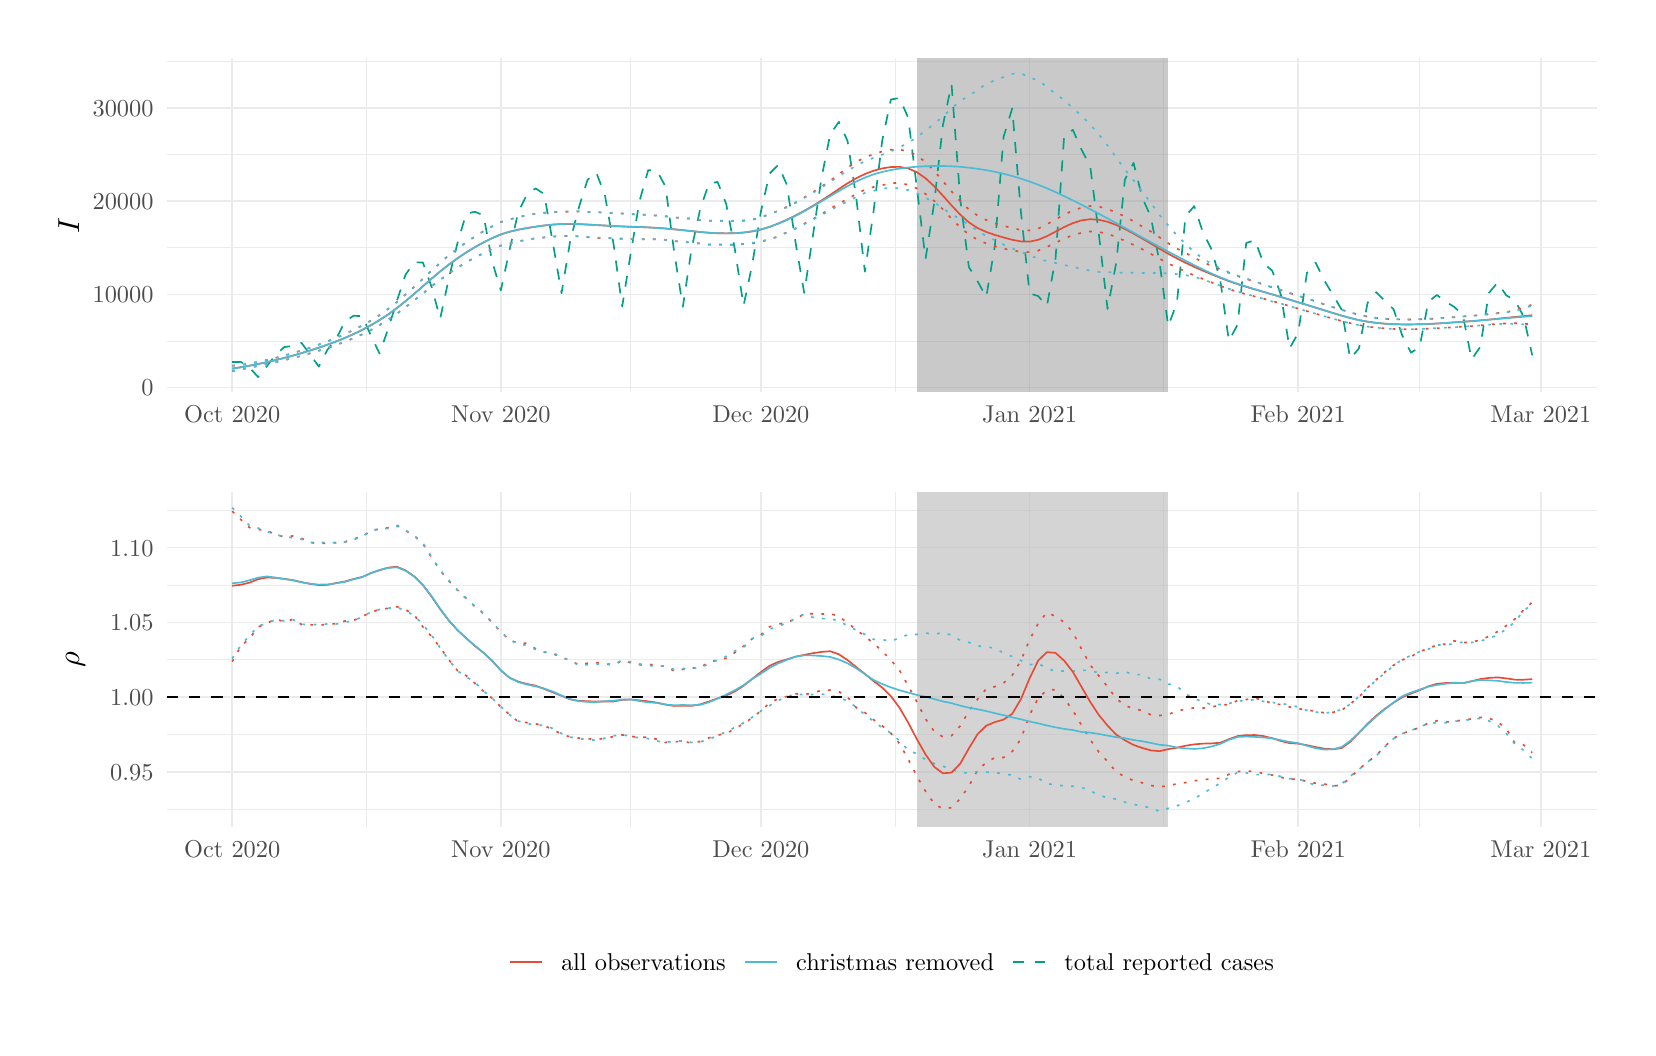
\begin{tikzpicture}[x=1pt,y=1pt]
\definecolor{fillColor}{RGB}{255,255,255}
\path[use as bounding box,fill=fillColor,fill opacity=0.00] (0,0) rectangle (578.16,361.35);
\begin{scope}
\path[clip] ( 50.41,229.59) rectangle (567.16,350.35);
\definecolor{drawColor}{gray}{0.92}

\path[draw=drawColor,line width= 0.3pt,line join=round] ( 50.41,248.14) --
	(567.16,248.14);

\path[draw=drawColor,line width= 0.3pt,line join=round] ( 50.41,281.80) --
	(567.16,281.80);

\path[draw=drawColor,line width= 0.3pt,line join=round] ( 50.41,315.47) --
	(567.16,315.47);

\path[draw=drawColor,line width= 0.3pt,line join=round] ( 50.41,349.13) --
	(567.16,349.13);

\path[draw=drawColor,line width= 0.3pt,line join=round] (122.44,229.59) --
	(122.44,350.35);

\path[draw=drawColor,line width= 0.3pt,line join=round] (217.96,229.59) --
	(217.96,350.35);

\path[draw=drawColor,line width= 0.3pt,line join=round] (313.48,229.59) --
	(313.48,350.35);

\path[draw=drawColor,line width= 0.3pt,line join=round] (410.57,229.59) --
	(410.57,350.35);

\path[draw=drawColor,line width= 0.3pt,line join=round] (502.96,229.59) --
	(502.96,350.35);

\path[draw=drawColor,line width= 0.6pt,line join=round] ( 50.41,231.31) --
	(567.16,231.31);

\path[draw=drawColor,line width= 0.6pt,line join=round] ( 50.41,264.97) --
	(567.16,264.97);

\path[draw=drawColor,line width= 0.6pt,line join=round] ( 50.41,298.63) --
	(567.16,298.63);

\path[draw=drawColor,line width= 0.6pt,line join=round] ( 50.41,332.30) --
	(567.16,332.30);

\path[draw=drawColor,line width= 0.6pt,line join=round] ( 73.90,229.59) --
	( 73.90,350.35);

\path[draw=drawColor,line width= 0.6pt,line join=round] (170.98,229.59) --
	(170.98,350.35);

\path[draw=drawColor,line width= 0.6pt,line join=round] (264.94,229.59) --
	(264.94,350.35);

\path[draw=drawColor,line width= 0.6pt,line join=round] (362.03,229.59) --
	(362.03,350.35);

\path[draw=drawColor,line width= 0.6pt,line join=round] (459.11,229.59) --
	(459.11,350.35);

\path[draw=drawColor,line width= 0.6pt,line join=round] (546.80,229.59) --
	(546.80,350.35);
\definecolor{fillColor}{RGB}{190,190,190}

\path[fill=fillColor,fill opacity=0.01] (321.31,229.59) rectangle (412.13,350.35);

\path[fill=fillColor,fill opacity=0.01] (321.31,229.59) rectangle (412.13,350.35);

\path[fill=fillColor,fill opacity=0.01] (321.31,229.59) rectangle (412.13,350.35);

\path[fill=fillColor,fill opacity=0.01] (321.31,229.59) rectangle (412.13,350.35);

\path[fill=fillColor,fill opacity=0.01] (321.31,229.59) rectangle (412.13,350.35);

\path[fill=fillColor,fill opacity=0.01] (321.31,229.59) rectangle (412.13,350.35);

\path[fill=fillColor,fill opacity=0.01] (321.31,229.59) rectangle (412.13,350.35);

\path[fill=fillColor,fill opacity=0.01] (321.31,229.59) rectangle (412.13,350.35);

\path[fill=fillColor,fill opacity=0.01] (321.31,229.59) rectangle (412.13,350.35);

\path[fill=fillColor,fill opacity=0.01] (321.31,229.59) rectangle (412.13,350.35);

\path[fill=fillColor,fill opacity=0.01] (321.31,229.59) rectangle (412.13,350.35);

\path[fill=fillColor,fill opacity=0.01] (321.31,229.59) rectangle (412.13,350.35);

\path[fill=fillColor,fill opacity=0.01] (321.31,229.59) rectangle (412.13,350.35);

\path[fill=fillColor,fill opacity=0.01] (321.31,229.59) rectangle (412.13,350.35);

\path[fill=fillColor,fill opacity=0.01] (321.31,229.59) rectangle (412.13,350.35);

\path[fill=fillColor,fill opacity=0.01] (321.31,229.59) rectangle (412.13,350.35);

\path[fill=fillColor,fill opacity=0.01] (321.31,229.59) rectangle (412.13,350.35);

\path[fill=fillColor,fill opacity=0.01] (321.31,229.59) rectangle (412.13,350.35);

\path[fill=fillColor,fill opacity=0.01] (321.31,229.59) rectangle (412.13,350.35);

\path[fill=fillColor,fill opacity=0.01] (321.31,229.59) rectangle (412.13,350.35);

\path[fill=fillColor,fill opacity=0.01] (321.31,229.59) rectangle (412.13,350.35);

\path[fill=fillColor,fill opacity=0.01] (321.31,229.59) rectangle (412.13,350.35);

\path[fill=fillColor,fill opacity=0.01] (321.31,229.59) rectangle (412.13,350.35);

\path[fill=fillColor,fill opacity=0.01] (321.31,229.59) rectangle (412.13,350.35);

\path[fill=fillColor,fill opacity=0.01] (321.31,229.59) rectangle (412.13,350.35);

\path[fill=fillColor,fill opacity=0.01] (321.31,229.59) rectangle (412.13,350.35);

\path[fill=fillColor,fill opacity=0.01] (321.31,229.59) rectangle (412.13,350.35);

\path[fill=fillColor,fill opacity=0.01] (321.31,229.59) rectangle (412.13,350.35);

\path[fill=fillColor,fill opacity=0.01] (321.31,229.59) rectangle (412.13,350.35);

\path[fill=fillColor,fill opacity=0.01] (321.31,229.59) rectangle (412.13,350.35);

\path[fill=fillColor,fill opacity=0.01] (321.31,229.59) rectangle (412.13,350.35);

\path[fill=fillColor,fill opacity=0.01] (321.31,229.59) rectangle (412.13,350.35);

\path[fill=fillColor,fill opacity=0.01] (321.31,229.59) rectangle (412.13,350.35);

\path[fill=fillColor,fill opacity=0.01] (321.31,229.59) rectangle (412.13,350.35);

\path[fill=fillColor,fill opacity=0.01] (321.31,229.59) rectangle (412.13,350.35);

\path[fill=fillColor,fill opacity=0.01] (321.31,229.59) rectangle (412.13,350.35);

\path[fill=fillColor,fill opacity=0.01] (321.31,229.59) rectangle (412.13,350.35);

\path[fill=fillColor,fill opacity=0.01] (321.31,229.59) rectangle (412.13,350.35);

\path[fill=fillColor,fill opacity=0.01] (321.31,229.59) rectangle (412.13,350.35);

\path[fill=fillColor,fill opacity=0.01] (321.31,229.59) rectangle (412.13,350.35);

\path[fill=fillColor,fill opacity=0.01] (321.31,229.59) rectangle (412.13,350.35);

\path[fill=fillColor,fill opacity=0.01] (321.31,229.59) rectangle (412.13,350.35);

\path[fill=fillColor,fill opacity=0.01] (321.31,229.59) rectangle (412.13,350.35);

\path[fill=fillColor,fill opacity=0.01] (321.31,229.59) rectangle (412.13,350.35);

\path[fill=fillColor,fill opacity=0.01] (321.31,229.59) rectangle (412.13,350.35);

\path[fill=fillColor,fill opacity=0.01] (321.31,229.59) rectangle (412.13,350.35);

\path[fill=fillColor,fill opacity=0.01] (321.31,229.59) rectangle (412.13,350.35);

\path[fill=fillColor,fill opacity=0.01] (321.31,229.59) rectangle (412.13,350.35);

\path[fill=fillColor,fill opacity=0.01] (321.31,229.59) rectangle (412.13,350.35);

\path[fill=fillColor,fill opacity=0.01] (321.31,229.59) rectangle (412.13,350.35);

\path[fill=fillColor,fill opacity=0.01] (321.31,229.59) rectangle (412.13,350.35);

\path[fill=fillColor,fill opacity=0.01] (321.31,229.59) rectangle (412.13,350.35);

\path[fill=fillColor,fill opacity=0.01] (321.31,229.59) rectangle (412.13,350.35);

\path[fill=fillColor,fill opacity=0.01] (321.31,229.59) rectangle (412.13,350.35);

\path[fill=fillColor,fill opacity=0.01] (321.31,229.59) rectangle (412.13,350.35);

\path[fill=fillColor,fill opacity=0.01] (321.31,229.59) rectangle (412.13,350.35);

\path[fill=fillColor,fill opacity=0.01] (321.31,229.59) rectangle (412.13,350.35);

\path[fill=fillColor,fill opacity=0.01] (321.31,229.59) rectangle (412.13,350.35);

\path[fill=fillColor,fill opacity=0.01] (321.31,229.59) rectangle (412.13,350.35);

\path[fill=fillColor,fill opacity=0.01] (321.31,229.59) rectangle (412.13,350.35);

\path[fill=fillColor,fill opacity=0.01] (321.31,229.59) rectangle (412.13,350.35);

\path[fill=fillColor,fill opacity=0.01] (321.31,229.59) rectangle (412.13,350.35);

\path[fill=fillColor,fill opacity=0.01] (321.31,229.59) rectangle (412.13,350.35);

\path[fill=fillColor,fill opacity=0.01] (321.31,229.59) rectangle (412.13,350.35);

\path[fill=fillColor,fill opacity=0.01] (321.31,229.59) rectangle (412.13,350.35);

\path[fill=fillColor,fill opacity=0.01] (321.31,229.59) rectangle (412.13,350.35);

\path[fill=fillColor,fill opacity=0.01] (321.31,229.59) rectangle (412.13,350.35);

\path[fill=fillColor,fill opacity=0.01] (321.31,229.59) rectangle (412.13,350.35);

\path[fill=fillColor,fill opacity=0.01] (321.31,229.59) rectangle (412.13,350.35);

\path[fill=fillColor,fill opacity=0.01] (321.31,229.59) rectangle (412.13,350.35);

\path[fill=fillColor,fill opacity=0.01] (321.31,229.59) rectangle (412.13,350.35);

\path[fill=fillColor,fill opacity=0.01] (321.31,229.59) rectangle (412.13,350.35);

\path[fill=fillColor,fill opacity=0.01] (321.31,229.59) rectangle (412.13,350.35);

\path[fill=fillColor,fill opacity=0.01] (321.31,229.59) rectangle (412.13,350.35);

\path[fill=fillColor,fill opacity=0.01] (321.31,229.59) rectangle (412.13,350.35);

\path[fill=fillColor,fill opacity=0.01] (321.31,229.59) rectangle (412.13,350.35);

\path[fill=fillColor,fill opacity=0.01] (321.31,229.59) rectangle (412.13,350.35);

\path[fill=fillColor,fill opacity=0.01] (321.31,229.59) rectangle (412.13,350.35);

\path[fill=fillColor,fill opacity=0.01] (321.31,229.59) rectangle (412.13,350.35);

\path[fill=fillColor,fill opacity=0.01] (321.31,229.59) rectangle (412.13,350.35);

\path[fill=fillColor,fill opacity=0.01] (321.31,229.59) rectangle (412.13,350.35);

\path[fill=fillColor,fill opacity=0.01] (321.31,229.59) rectangle (412.13,350.35);

\path[fill=fillColor,fill opacity=0.01] (321.31,229.59) rectangle (412.13,350.35);

\path[fill=fillColor,fill opacity=0.01] (321.31,229.59) rectangle (412.13,350.35);

\path[fill=fillColor,fill opacity=0.01] (321.31,229.59) rectangle (412.13,350.35);

\path[fill=fillColor,fill opacity=0.01] (321.31,229.59) rectangle (412.13,350.35);

\path[fill=fillColor,fill opacity=0.01] (321.31,229.59) rectangle (412.13,350.35);

\path[fill=fillColor,fill opacity=0.01] (321.31,229.59) rectangle (412.13,350.35);

\path[fill=fillColor,fill opacity=0.01] (321.31,229.59) rectangle (412.13,350.35);

\path[fill=fillColor,fill opacity=0.01] (321.31,229.59) rectangle (412.13,350.35);

\path[fill=fillColor,fill opacity=0.01] (321.31,229.59) rectangle (412.13,350.35);

\path[fill=fillColor,fill opacity=0.01] (321.31,229.59) rectangle (412.13,350.35);

\path[fill=fillColor,fill opacity=0.01] (321.31,229.59) rectangle (412.13,350.35);

\path[fill=fillColor,fill opacity=0.01] (321.31,229.59) rectangle (412.13,350.35);

\path[fill=fillColor,fill opacity=0.01] (321.31,229.59) rectangle (412.13,350.35);

\path[fill=fillColor,fill opacity=0.01] (321.31,229.59) rectangle (412.13,350.35);

\path[fill=fillColor,fill opacity=0.01] (321.31,229.59) rectangle (412.13,350.35);

\path[fill=fillColor,fill opacity=0.01] (321.31,229.59) rectangle (412.13,350.35);

\path[fill=fillColor,fill opacity=0.01] (321.31,229.59) rectangle (412.13,350.35);

\path[fill=fillColor,fill opacity=0.01] (321.31,229.59) rectangle (412.13,350.35);

\path[fill=fillColor,fill opacity=0.01] (321.31,229.59) rectangle (412.13,350.35);

\path[fill=fillColor,fill opacity=0.01] (321.31,229.59) rectangle (412.13,350.35);

\path[fill=fillColor,fill opacity=0.01] (321.31,229.59) rectangle (412.13,350.35);

\path[fill=fillColor,fill opacity=0.01] (321.31,229.59) rectangle (412.13,350.35);

\path[fill=fillColor,fill opacity=0.01] (321.31,229.59) rectangle (412.13,350.35);

\path[fill=fillColor,fill opacity=0.01] (321.31,229.59) rectangle (412.13,350.35);

\path[fill=fillColor,fill opacity=0.01] (321.31,229.59) rectangle (412.13,350.35);

\path[fill=fillColor,fill opacity=0.01] (321.31,229.59) rectangle (412.13,350.35);

\path[fill=fillColor,fill opacity=0.01] (321.31,229.59) rectangle (412.13,350.35);

\path[fill=fillColor,fill opacity=0.01] (321.31,229.59) rectangle (412.13,350.35);

\path[fill=fillColor,fill opacity=0.01] (321.31,229.59) rectangle (412.13,350.35);

\path[fill=fillColor,fill opacity=0.01] (321.31,229.59) rectangle (412.13,350.35);

\path[fill=fillColor,fill opacity=0.01] (321.31,229.59) rectangle (412.13,350.35);

\path[fill=fillColor,fill opacity=0.01] (321.31,229.59) rectangle (412.13,350.35);

\path[fill=fillColor,fill opacity=0.01] (321.31,229.59) rectangle (412.13,350.35);

\path[fill=fillColor,fill opacity=0.01] (321.31,229.59) rectangle (412.13,350.35);

\path[fill=fillColor,fill opacity=0.01] (321.31,229.59) rectangle (412.13,350.35);

\path[fill=fillColor,fill opacity=0.01] (321.31,229.59) rectangle (412.13,350.35);

\path[fill=fillColor,fill opacity=0.01] (321.31,229.59) rectangle (412.13,350.35);

\path[fill=fillColor,fill opacity=0.01] (321.31,229.59) rectangle (412.13,350.35);

\path[fill=fillColor,fill opacity=0.01] (321.31,229.59) rectangle (412.13,350.35);

\path[fill=fillColor,fill opacity=0.01] (321.31,229.59) rectangle (412.13,350.35);

\path[fill=fillColor,fill opacity=0.01] (321.31,229.59) rectangle (412.13,350.35);

\path[fill=fillColor,fill opacity=0.01] (321.31,229.59) rectangle (412.13,350.35);

\path[fill=fillColor,fill opacity=0.01] (321.31,229.59) rectangle (412.13,350.35);

\path[fill=fillColor,fill opacity=0.01] (321.31,229.59) rectangle (412.13,350.35);

\path[fill=fillColor,fill opacity=0.01] (321.31,229.59) rectangle (412.13,350.35);

\path[fill=fillColor,fill opacity=0.01] (321.31,229.59) rectangle (412.13,350.35);

\path[fill=fillColor,fill opacity=0.01] (321.31,229.59) rectangle (412.13,350.35);

\path[fill=fillColor,fill opacity=0.01] (321.31,229.59) rectangle (412.13,350.35);

\path[fill=fillColor,fill opacity=0.01] (321.31,229.59) rectangle (412.13,350.35);

\path[fill=fillColor,fill opacity=0.01] (321.31,229.59) rectangle (412.13,350.35);

\path[fill=fillColor,fill opacity=0.01] (321.31,229.59) rectangle (412.13,350.35);

\path[fill=fillColor,fill opacity=0.01] (321.31,229.59) rectangle (412.13,350.35);

\path[fill=fillColor,fill opacity=0.01] (321.31,229.59) rectangle (412.13,350.35);

\path[fill=fillColor,fill opacity=0.01] (321.31,229.59) rectangle (412.13,350.35);

\path[fill=fillColor,fill opacity=0.01] (321.31,229.59) rectangle (412.13,350.35);

\path[fill=fillColor,fill opacity=0.01] (321.31,229.59) rectangle (412.13,350.35);

\path[fill=fillColor,fill opacity=0.01] (321.31,229.59) rectangle (412.13,350.35);

\path[fill=fillColor,fill opacity=0.01] (321.31,229.59) rectangle (412.13,350.35);

\path[fill=fillColor,fill opacity=0.01] (321.31,229.59) rectangle (412.13,350.35);

\path[fill=fillColor,fill opacity=0.01] (321.31,229.59) rectangle (412.13,350.35);

\path[fill=fillColor,fill opacity=0.01] (321.31,229.59) rectangle (412.13,350.35);

\path[fill=fillColor,fill opacity=0.01] (321.31,229.59) rectangle (412.13,350.35);

\path[fill=fillColor,fill opacity=0.01] (321.31,229.59) rectangle (412.13,350.35);

\path[fill=fillColor,fill opacity=0.01] (321.31,229.59) rectangle (412.13,350.35);

\path[fill=fillColor,fill opacity=0.01] (321.31,229.59) rectangle (412.13,350.35);

\path[fill=fillColor,fill opacity=0.01] (321.31,229.59) rectangle (412.13,350.35);

\path[fill=fillColor,fill opacity=0.01] (321.31,229.59) rectangle (412.13,350.35);

\path[fill=fillColor,fill opacity=0.01] (321.31,229.59) rectangle (412.13,350.35);

\path[fill=fillColor,fill opacity=0.01] (321.31,229.59) rectangle (412.13,350.35);

\path[fill=fillColor,fill opacity=0.01] (321.31,229.59) rectangle (412.13,350.35);

\path[fill=fillColor,fill opacity=0.01] (321.31,229.59) rectangle (412.13,350.35);

\path[fill=fillColor,fill opacity=0.01] (321.31,229.59) rectangle (412.13,350.35);

\path[fill=fillColor,fill opacity=0.01] (321.31,229.59) rectangle (412.13,350.35);

\path[fill=fillColor,fill opacity=0.01] (321.31,229.59) rectangle (412.13,350.35);

\path[fill=fillColor,fill opacity=0.01] (321.31,229.59) rectangle (412.13,350.35);

\path[fill=fillColor,fill opacity=0.01] (321.31,229.59) rectangle (412.13,350.35);

\path[fill=fillColor,fill opacity=0.01] (321.31,229.59) rectangle (412.13,350.35);

\path[fill=fillColor,fill opacity=0.01] (321.31,229.59) rectangle (412.13,350.35);

\path[fill=fillColor,fill opacity=0.01] (321.31,229.59) rectangle (412.13,350.35);

\path[fill=fillColor,fill opacity=0.01] (321.31,229.59) rectangle (412.13,350.35);

\path[fill=fillColor,fill opacity=0.01] (321.31,229.59) rectangle (412.13,350.35);

\path[fill=fillColor,fill opacity=0.01] (321.31,229.59) rectangle (412.13,350.35);

\path[fill=fillColor,fill opacity=0.01] (321.31,229.59) rectangle (412.13,350.35);

\path[fill=fillColor,fill opacity=0.01] (321.31,229.59) rectangle (412.13,350.35);

\path[fill=fillColor,fill opacity=0.01] (321.31,229.59) rectangle (412.13,350.35);

\path[fill=fillColor,fill opacity=0.01] (321.31,229.59) rectangle (412.13,350.35);

\path[fill=fillColor,fill opacity=0.01] (321.31,229.59) rectangle (412.13,350.35);

\path[fill=fillColor,fill opacity=0.01] (321.31,229.59) rectangle (412.13,350.35);

\path[fill=fillColor,fill opacity=0.01] (321.31,229.59) rectangle (412.13,350.35);

\path[fill=fillColor,fill opacity=0.01] (321.31,229.59) rectangle (412.13,350.35);

\path[fill=fillColor,fill opacity=0.01] (321.31,229.59) rectangle (412.13,350.35);

\path[fill=fillColor,fill opacity=0.01] (321.31,229.59) rectangle (412.13,350.35);

\path[fill=fillColor,fill opacity=0.01] (321.31,229.59) rectangle (412.13,350.35);

\path[fill=fillColor,fill opacity=0.01] (321.31,229.59) rectangle (412.13,350.35);

\path[fill=fillColor,fill opacity=0.01] (321.31,229.59) rectangle (412.13,350.35);

\path[fill=fillColor,fill opacity=0.01] (321.31,229.59) rectangle (412.13,350.35);

\path[fill=fillColor,fill opacity=0.01] (321.31,229.59) rectangle (412.13,350.35);

\path[fill=fillColor,fill opacity=0.01] (321.31,229.59) rectangle (412.13,350.35);

\path[fill=fillColor,fill opacity=0.01] (321.31,229.59) rectangle (412.13,350.35);

\path[fill=fillColor,fill opacity=0.01] (321.31,229.59) rectangle (412.13,350.35);

\path[fill=fillColor,fill opacity=0.01] (321.31,229.59) rectangle (412.13,350.35);

\path[fill=fillColor,fill opacity=0.01] (321.31,229.59) rectangle (412.13,350.35);

\path[fill=fillColor,fill opacity=0.01] (321.31,229.59) rectangle (412.13,350.35);

\path[fill=fillColor,fill opacity=0.01] (321.31,229.59) rectangle (412.13,350.35);

\path[fill=fillColor,fill opacity=0.01] (321.31,229.59) rectangle (412.13,350.35);

\path[fill=fillColor,fill opacity=0.01] (321.31,229.59) rectangle (412.13,350.35);

\path[fill=fillColor,fill opacity=0.01] (321.31,229.59) rectangle (412.13,350.35);

\path[fill=fillColor,fill opacity=0.01] (321.31,229.59) rectangle (412.13,350.35);

\path[fill=fillColor,fill opacity=0.01] (321.31,229.59) rectangle (412.13,350.35);

\path[fill=fillColor,fill opacity=0.01] (321.31,229.59) rectangle (412.13,350.35);

\path[fill=fillColor,fill opacity=0.01] (321.31,229.59) rectangle (412.13,350.35);

\path[fill=fillColor,fill opacity=0.01] (321.31,229.59) rectangle (412.13,350.35);

\path[fill=fillColor,fill opacity=0.01] (321.31,229.59) rectangle (412.13,350.35);

\path[fill=fillColor,fill opacity=0.01] (321.31,229.59) rectangle (412.13,350.35);

\path[fill=fillColor,fill opacity=0.01] (321.31,229.59) rectangle (412.13,350.35);

\path[fill=fillColor,fill opacity=0.01] (321.31,229.59) rectangle (412.13,350.35);

\path[fill=fillColor,fill opacity=0.01] (321.31,229.59) rectangle (412.13,350.35);

\path[fill=fillColor,fill opacity=0.01] (321.31,229.59) rectangle (412.13,350.35);

\path[fill=fillColor,fill opacity=0.01] (321.31,229.59) rectangle (412.13,350.35);

\path[fill=fillColor,fill opacity=0.01] (321.31,229.59) rectangle (412.13,350.35);

\path[fill=fillColor,fill opacity=0.01] (321.31,229.59) rectangle (412.13,350.35);

\path[fill=fillColor,fill opacity=0.01] (321.31,229.59) rectangle (412.13,350.35);

\path[fill=fillColor,fill opacity=0.01] (321.31,229.59) rectangle (412.13,350.35);

\path[fill=fillColor,fill opacity=0.01] (321.31,229.59) rectangle (412.13,350.35);

\path[fill=fillColor,fill opacity=0.01] (321.31,229.59) rectangle (412.13,350.35);

\path[fill=fillColor,fill opacity=0.01] (321.31,229.59) rectangle (412.13,350.35);

\path[fill=fillColor,fill opacity=0.01] (321.31,229.59) rectangle (412.13,350.35);

\path[fill=fillColor,fill opacity=0.01] (321.31,229.59) rectangle (412.13,350.35);

\path[fill=fillColor,fill opacity=0.01] (321.31,229.59) rectangle (412.13,350.35);

\path[fill=fillColor,fill opacity=0.01] (321.31,229.59) rectangle (412.13,350.35);

\path[fill=fillColor,fill opacity=0.01] (321.31,229.59) rectangle (412.13,350.35);

\path[fill=fillColor,fill opacity=0.01] (321.31,229.59) rectangle (412.13,350.35);

\path[fill=fillColor,fill opacity=0.01] (321.31,229.59) rectangle (412.13,350.35);

\path[fill=fillColor,fill opacity=0.01] (321.31,229.59) rectangle (412.13,350.35);

\path[fill=fillColor,fill opacity=0.01] (321.31,229.59) rectangle (412.13,350.35);

\path[fill=fillColor,fill opacity=0.01] (321.31,229.59) rectangle (412.13,350.35);

\path[fill=fillColor,fill opacity=0.01] (321.31,229.59) rectangle (412.13,350.35);

\path[fill=fillColor,fill opacity=0.01] (321.31,229.59) rectangle (412.13,350.35);

\path[fill=fillColor,fill opacity=0.01] (321.31,229.59) rectangle (412.13,350.35);

\path[fill=fillColor,fill opacity=0.01] (321.31,229.59) rectangle (412.13,350.35);

\path[fill=fillColor,fill opacity=0.01] (321.31,229.59) rectangle (412.13,350.35);

\path[fill=fillColor,fill opacity=0.01] (321.31,229.59) rectangle (412.13,350.35);

\path[fill=fillColor,fill opacity=0.01] (321.31,229.59) rectangle (412.13,350.35);

\path[fill=fillColor,fill opacity=0.01] (321.31,229.59) rectangle (412.13,350.35);

\path[fill=fillColor,fill opacity=0.01] (321.31,229.59) rectangle (412.13,350.35);

\path[fill=fillColor,fill opacity=0.01] (321.31,229.59) rectangle (412.13,350.35);

\path[fill=fillColor,fill opacity=0.01] (321.31,229.59) rectangle (412.13,350.35);

\path[fill=fillColor,fill opacity=0.01] (321.31,229.59) rectangle (412.13,350.35);

\path[fill=fillColor,fill opacity=0.01] (321.31,229.59) rectangle (412.13,350.35);

\path[fill=fillColor,fill opacity=0.01] (321.31,229.59) rectangle (412.13,350.35);

\path[fill=fillColor,fill opacity=0.01] (321.31,229.59) rectangle (412.13,350.35);

\path[fill=fillColor,fill opacity=0.01] (321.31,229.59) rectangle (412.13,350.35);

\path[fill=fillColor,fill opacity=0.01] (321.31,229.59) rectangle (412.13,350.35);

\path[fill=fillColor,fill opacity=0.01] (321.31,229.59) rectangle (412.13,350.35);

\path[fill=fillColor,fill opacity=0.01] (321.31,229.59) rectangle (412.13,350.35);

\path[fill=fillColor,fill opacity=0.01] (321.31,229.59) rectangle (412.13,350.35);

\path[fill=fillColor,fill opacity=0.01] (321.31,229.59) rectangle (412.13,350.35);

\path[fill=fillColor,fill opacity=0.01] (321.31,229.59) rectangle (412.13,350.35);

\path[fill=fillColor,fill opacity=0.01] (321.31,229.59) rectangle (412.13,350.35);

\path[fill=fillColor,fill opacity=0.01] (321.31,229.59) rectangle (412.13,350.35);

\path[fill=fillColor,fill opacity=0.01] (321.31,229.59) rectangle (412.13,350.35);

\path[fill=fillColor,fill opacity=0.01] (321.31,229.59) rectangle (412.13,350.35);

\path[fill=fillColor,fill opacity=0.01] (321.31,229.59) rectangle (412.13,350.35);

\path[fill=fillColor,fill opacity=0.01] (321.31,229.59) rectangle (412.13,350.35);

\path[fill=fillColor,fill opacity=0.01] (321.31,229.59) rectangle (412.13,350.35);

\path[fill=fillColor,fill opacity=0.01] (321.31,229.59) rectangle (412.13,350.35);

\path[fill=fillColor,fill opacity=0.01] (321.31,229.59) rectangle (412.13,350.35);

\path[fill=fillColor,fill opacity=0.01] (321.31,229.59) rectangle (412.13,350.35);

\path[fill=fillColor,fill opacity=0.01] (321.31,229.59) rectangle (412.13,350.35);

\path[fill=fillColor,fill opacity=0.01] (321.31,229.59) rectangle (412.13,350.35);

\path[fill=fillColor,fill opacity=0.01] (321.31,229.59) rectangle (412.13,350.35);

\path[fill=fillColor,fill opacity=0.01] (321.31,229.59) rectangle (412.13,350.35);

\path[fill=fillColor,fill opacity=0.01] (321.31,229.59) rectangle (412.13,350.35);

\path[fill=fillColor,fill opacity=0.01] (321.31,229.59) rectangle (412.13,350.35);

\path[fill=fillColor,fill opacity=0.01] (321.31,229.59) rectangle (412.13,350.35);

\path[fill=fillColor,fill opacity=0.01] (321.31,229.59) rectangle (412.13,350.35);

\path[fill=fillColor,fill opacity=0.01] (321.31,229.59) rectangle (412.13,350.35);

\path[fill=fillColor,fill opacity=0.01] (321.31,229.59) rectangle (412.13,350.35);

\path[fill=fillColor,fill opacity=0.01] (321.31,229.59) rectangle (412.13,350.35);

\path[fill=fillColor,fill opacity=0.01] (321.31,229.59) rectangle (412.13,350.35);

\path[fill=fillColor,fill opacity=0.01] (321.31,229.59) rectangle (412.13,350.35);

\path[fill=fillColor,fill opacity=0.01] (321.31,229.59) rectangle (412.13,350.35);

\path[fill=fillColor,fill opacity=0.01] (321.31,229.59) rectangle (412.13,350.35);

\path[fill=fillColor,fill opacity=0.01] (321.31,229.59) rectangle (412.13,350.35);

\path[fill=fillColor,fill opacity=0.01] (321.31,229.59) rectangle (412.13,350.35);

\path[fill=fillColor,fill opacity=0.01] (321.31,229.59) rectangle (412.13,350.35);

\path[fill=fillColor,fill opacity=0.01] (321.31,229.59) rectangle (412.13,350.35);

\path[fill=fillColor,fill opacity=0.01] (321.31,229.59) rectangle (412.13,350.35);

\path[fill=fillColor,fill opacity=0.01] (321.31,229.59) rectangle (412.13,350.35);

\path[fill=fillColor,fill opacity=0.01] (321.31,229.59) rectangle (412.13,350.35);

\path[fill=fillColor,fill opacity=0.01] (321.31,229.59) rectangle (412.13,350.35);

\path[fill=fillColor,fill opacity=0.01] (321.31,229.59) rectangle (412.13,350.35);

\path[fill=fillColor,fill opacity=0.01] (321.31,229.59) rectangle (412.13,350.35);

\path[fill=fillColor,fill opacity=0.01] (321.31,229.59) rectangle (412.13,350.35);

\path[fill=fillColor,fill opacity=0.01] (321.31,229.59) rectangle (412.13,350.35);

\path[fill=fillColor,fill opacity=0.01] (321.31,229.59) rectangle (412.13,350.35);

\path[fill=fillColor,fill opacity=0.01] (321.31,229.59) rectangle (412.13,350.35);

\path[fill=fillColor,fill opacity=0.01] (321.31,229.59) rectangle (412.13,350.35);

\path[fill=fillColor,fill opacity=0.01] (321.31,229.59) rectangle (412.13,350.35);

\path[fill=fillColor,fill opacity=0.01] (321.31,229.59) rectangle (412.13,350.35);

\path[fill=fillColor,fill opacity=0.01] (321.31,229.59) rectangle (412.13,350.35);

\path[fill=fillColor,fill opacity=0.01] (321.31,229.59) rectangle (412.13,350.35);

\path[fill=fillColor,fill opacity=0.01] (321.31,229.59) rectangle (412.13,350.35);

\path[fill=fillColor,fill opacity=0.01] (321.31,229.59) rectangle (412.13,350.35);

\path[fill=fillColor,fill opacity=0.01] (321.31,229.59) rectangle (412.13,350.35);

\path[fill=fillColor,fill opacity=0.01] (321.31,229.59) rectangle (412.13,350.35);

\path[fill=fillColor,fill opacity=0.01] (321.31,229.59) rectangle (412.13,350.35);

\path[fill=fillColor,fill opacity=0.01] (321.31,229.59) rectangle (412.13,350.35);

\path[fill=fillColor,fill opacity=0.01] (321.31,229.59) rectangle (412.13,350.35);

\path[fill=fillColor,fill opacity=0.01] (321.31,229.59) rectangle (412.13,350.35);

\path[fill=fillColor,fill opacity=0.01] (321.31,229.59) rectangle (412.13,350.35);

\path[fill=fillColor,fill opacity=0.01] (321.31,229.59) rectangle (412.13,350.35);

\path[fill=fillColor,fill opacity=0.01] (321.31,229.59) rectangle (412.13,350.35);

\path[fill=fillColor,fill opacity=0.01] (321.31,229.59) rectangle (412.13,350.35);

\path[fill=fillColor,fill opacity=0.01] (321.31,229.59) rectangle (412.13,350.35);

\path[fill=fillColor,fill opacity=0.01] (321.31,229.59) rectangle (412.13,350.35);

\path[fill=fillColor,fill opacity=0.01] (321.31,229.59) rectangle (412.13,350.35);

\path[fill=fillColor,fill opacity=0.01] (321.31,229.59) rectangle (412.13,350.35);

\path[fill=fillColor,fill opacity=0.01] (321.31,229.59) rectangle (412.13,350.35);

\path[fill=fillColor,fill opacity=0.01] (321.31,229.59) rectangle (412.13,350.35);
\definecolor{drawColor}{RGB}{0,160,135}

\path[draw=drawColor,line width= 0.6pt,dash pattern=on 4pt off 4pt ,line join=round] ( 73.90,240.54) --
	( 77.03,240.57) --
	( 80.16,238.51) --
	( 83.29,235.08) --
	( 86.43,239.04) --
	( 89.56,243.09) --
	( 92.69,245.93) --
	( 95.82,246.34) --
	( 98.95,247.45) --
	(102.08,243.17) --
	(105.22,238.87) --
	(108.35,245.04) --
	(111.48,248.91) --
	(114.61,255.12) --
	(117.74,257.24) --
	(120.88,257.11) --
	(124.01,250.13) --
	(127.14,243.62) --
	(130.27,252.56) --
	(133.40,262.57) --
	(136.53,272.08) --
	(139.67,276.55) --
	(142.80,276.50) --
	(145.93,267.76) --
	(149.06,256.21) --
	(152.19,270.75) --
	(155.33,283.60) --
	(158.46,294.14) --
	(161.59,294.82) --
	(164.72,293.55) --
	(167.85,276.77) --
	(170.98,266.44) --
	(174.12,281.03) --
	(177.25,294.63) --
	(180.38,301.04) --
	(183.51,303.28) --
	(186.64,301.22) --
	(189.78,283.53) --
	(192.91,265.40) --
	(196.04,284.33) --
	(199.17,296.39) --
	(202.30,306.36) --
	(205.43,309.05) --
	(208.57,300.94) --
	(211.70,283.19) --
	(214.83,260.60) --
	(217.96,280.12) --
	(221.09,298.69) --
	(224.23,309.88) --
	(227.36,309.72) --
	(230.49,303.89) --
	(233.62,280.21) --
	(236.75,260.50) --
	(239.88,281.41) --
	(243.02,295.87) --
	(246.15,304.95) --
	(249.28,305.63) --
	(252.41,297.65) --
	(255.54,281.25) --
	(258.68,260.87) --
	(261.81,275.75) --
	(264.94,294.85) --
	(268.07,308.63) --
	(271.20,311.73) --
	(274.33,304.57) --
	(277.47,283.74) --
	(280.60,265.50) --
	(283.73,286.12) --
	(286.86,307.13) --
	(289.99,322.82) --
	(293.13,327.31) --
	(296.26,320.37) --
	(299.39,300.03) --
	(302.52,273.16) --
	(305.65,294.95) --
	(308.78,320.51) --
	(311.92,335.40) --
	(315.05,335.91) --
	(318.18,328.77) --
	(321.31,303.45) --
	(324.44,277.74) --
	(327.58,298.10) --
	(330.71,326.08) --
	(333.84,340.90) --
	(336.97,299.47) --
	(340.10,274.85) --
	(343.23,269.73) --
	(346.37,263.97) --
	(349.50,282.58) --
	(352.63,321.83) --
	(355.76,332.18) --
	(358.89,294.94) --
	(362.03,265.35) --
	(365.16,264.35) --
	(368.29,260.73) --
	(371.42,277.97) --
	(374.55,322.47) --
	(377.68,324.40) --
	(380.82,317.22) --
	(383.95,311.29) --
	(387.08,286.63) --
	(390.21,259.69) --
	(393.34,276.40) --
	(396.48,306.46) --
	(399.61,312.49) --
	(402.74,299.97) --
	(405.87,292.94) --
	(409.00,276.52) --
	(412.13,253.51) --
	(415.27,261.93) --
	(418.40,293.26) --
	(421.53,296.86) --
	(424.66,287.49) --
	(427.79,281.24) --
	(430.93,270.13) --
	(434.06,248.19) --
	(437.19,254.03) --
	(440.32,283.55) --
	(443.45,284.55) --
	(446.58,276.18) --
	(449.72,273.52) --
	(452.85,264.81) --
	(455.98,245.45) --
	(459.11,251.05) --
	(462.24,272.72) --
	(465.38,276.46) --
	(468.51,270.06) --
	(471.64,264.78) --
	(474.77,259.52) --
	(477.90,241.72) --
	(481.03,245.42) --
	(484.17,261.91) --
	(487.30,265.76) --
	(490.43,262.63) --
	(493.56,259.61) --
	(496.69,250.12) --
	(499.83,243.91) --
	(502.96,245.86) --
	(506.09,262.24) --
	(509.22,264.77) --
	(512.35,262.32) --
	(515.48,260.47) --
	(518.62,257.37) --
	(521.75,241.49) --
	(524.88,245.98) --
	(528.01,265.53) --
	(531.14,269.22) --
	(534.28,264.63) --
	(537.41,262.80) --
	(540.54,256.99) --
	(543.67,242.93);
\definecolor{drawColor}{RGB}{230,75,53}

\path[draw=drawColor,line width= 0.6pt,dash pattern=on 1pt off 3pt ,line join=round] ( 73.90,237.26) --
	( 77.03,237.88) --
	( 80.16,238.50) --
	( 83.29,239.13) --
	( 86.43,239.77) --
	( 89.56,240.46) --
	( 92.69,241.19) --
	( 95.82,241.96) --
	( 98.95,242.75) --
	(102.08,243.69) --
	(105.22,244.62) --
	(108.35,245.63) --
	(111.48,246.71) --
	(114.61,247.86) --
	(117.74,249.13) --
	(120.88,250.52) --
	(124.01,252.05) --
	(127.14,253.87) --
	(130.27,255.84) --
	(133.40,257.98) --
	(136.53,260.32) --
	(139.67,262.86) --
	(142.80,265.32) --
	(145.93,267.87) --
	(149.06,270.28) --
	(152.19,272.48) --
	(155.33,274.63) --
	(158.46,276.54) --
	(161.59,278.30) --
	(164.72,279.85) --
	(167.85,281.42) --
	(170.98,282.61) --
	(174.12,283.30) --
	(177.25,284.13) --
	(180.38,284.70) --
	(183.51,285.24) --
	(186.64,285.54) --
	(189.78,285.85) --
	(192.91,286.05) --
	(196.04,286.11) --
	(199.17,285.89) --
	(202.30,285.66) --
	(205.43,285.35) --
	(208.57,285.34) --
	(211.70,285.21) --
	(214.83,285.06) --
	(217.96,285.01) --
	(221.09,284.93) --
	(224.23,284.81) --
	(227.36,284.91) --
	(230.49,284.67) --
	(233.62,284.25) --
	(236.75,283.91) --
	(239.88,283.69) --
	(243.02,283.36) --
	(246.15,282.98) --
	(249.28,283.01) --
	(252.41,282.90) --
	(255.54,282.87) --
	(258.68,283.12) --
	(261.81,283.36) --
	(264.94,284.05) --
	(268.07,284.84) --
	(271.20,285.94) --
	(274.33,287.43) --
	(277.47,288.79) --
	(280.60,290.52) --
	(283.73,292.18) --
	(286.86,293.94) --
	(289.99,295.94) --
	(293.13,297.72) --
	(296.26,299.52) --
	(299.39,301.21) --
	(302.52,302.83) --
	(305.65,303.77) --
	(308.78,304.42) --
	(311.92,305.22) --
	(315.05,305.25) --
	(318.18,304.56) --
	(321.31,303.27) --
	(324.44,301.26) --
	(327.58,298.75) --
	(330.71,295.68) --
	(333.84,292.33) --
	(336.97,289.19) --
	(340.10,286.60) --
	(343.23,284.73) --
	(346.37,283.38) --
	(349.50,282.33) --
	(352.63,281.50) --
	(355.76,280.86) --
	(358.89,280.37) --
	(362.03,280.23) --
	(365.16,280.77) --
	(368.29,282.10) --
	(371.42,283.60) --
	(374.55,285.14) --
	(377.68,286.37) --
	(380.82,287.23) --
	(383.95,287.71) --
	(387.08,287.50) --
	(390.21,286.85) --
	(393.34,285.73) --
	(396.48,284.29) --
	(399.61,282.84) --
	(402.74,281.29) --
	(405.87,279.58) --
	(409.00,277.86) --
	(412.13,276.18) --
	(415.27,274.67) --
	(418.40,273.22) --
	(421.53,271.83) --
	(424.66,270.56) --
	(427.79,269.28) --
	(430.93,268.03) --
	(434.06,266.89) --
	(437.19,265.89) --
	(440.32,265.02) --
	(443.45,264.22) --
	(446.58,263.41) --
	(449.72,262.54) --
	(452.85,261.75) --
	(455.98,260.72) --
	(459.11,259.81) --
	(462.24,258.92) --
	(465.38,258.01) --
	(468.51,257.06) --
	(471.64,256.23) --
	(474.77,255.36) --
	(477.90,254.56) --
	(481.03,253.88) --
	(484.17,253.32) --
	(487.30,252.94) --
	(490.43,252.70) --
	(493.56,252.50) --
	(496.69,252.36) --
	(499.83,252.38) --
	(502.96,252.46) --
	(506.09,252.55) --
	(509.22,252.73) --
	(512.35,252.94) --
	(515.48,253.08) --
	(518.62,253.34) --
	(521.75,253.51) --
	(524.88,253.77) --
	(528.01,254.03) --
	(531.14,254.32) --
	(534.28,254.49) --
	(537.41,254.57) --
	(540.54,254.39) --
	(543.67,254.08);
\definecolor{drawColor}{RGB}{77,187,213}

\path[draw=drawColor,line width= 0.6pt,dash pattern=on 1pt off 3pt ,line join=round] ( 73.90,237.19) --
	( 77.03,237.84) --
	( 80.16,238.48) --
	( 83.29,239.11) --
	( 86.43,239.77) --
	( 89.56,240.46) --
	( 92.69,241.21) --
	( 95.82,241.97) --
	( 98.95,242.79) --
	(102.08,243.70) --
	(105.22,244.64) --
	(108.35,245.65) --
	(111.48,246.73) --
	(114.61,247.87) --
	(117.74,249.13) --
	(120.88,250.55) --
	(124.01,252.10) --
	(127.14,253.89) --
	(130.27,255.85) --
	(133.40,257.97) --
	(136.53,260.32) --
	(139.67,262.82) --
	(142.80,265.26) --
	(145.93,267.84) --
	(149.06,270.28) --
	(152.19,272.53) --
	(155.33,274.66) --
	(158.46,276.55) --
	(161.59,278.33) --
	(164.72,279.89) --
	(167.85,281.37) --
	(170.98,282.60) --
	(174.12,283.32) --
	(177.25,284.12) --
	(180.38,284.69) --
	(183.51,285.25) --
	(186.64,285.58) --
	(189.78,285.90) --
	(192.91,286.09) --
	(196.04,286.16) --
	(199.17,285.98) --
	(202.30,285.78) --
	(205.43,285.52) --
	(208.57,285.41) --
	(211.70,285.28) --
	(214.83,285.13) --
	(217.96,285.07) --
	(221.09,284.97) --
	(224.23,284.85) --
	(227.36,284.88) --
	(230.49,284.65) --
	(233.62,284.21) --
	(236.75,283.91) --
	(239.88,283.67) --
	(243.02,283.33) --
	(246.15,282.94) --
	(249.28,282.90) --
	(252.41,282.87) --
	(255.54,282.95) --
	(258.68,283.23) --
	(261.81,283.60) --
	(264.94,284.16) --
	(268.07,284.84) --
	(271.20,285.87) --
	(274.33,287.36) --
	(277.47,288.72) --
	(280.60,290.36) --
	(283.73,291.99) --
	(286.86,293.60) --
	(289.99,295.40) --
	(293.13,297.04) --
	(296.26,298.58) --
	(299.39,300.14) --
	(302.52,301.63) --
	(305.65,302.37) --
	(308.78,303.21) --
	(311.92,303.45) --
	(315.05,303.28) --
	(318.18,302.66) --
	(321.31,301.46) --
	(324.44,299.88) --
	(327.58,298.20) --
	(330.71,296.06) --
	(333.84,293.91) --
	(336.97,292.18) --
	(340.10,290.05) --
	(343.23,288.10) --
	(346.37,286.00) --
	(349.50,284.54) --
	(352.63,282.95) --
	(355.76,281.56) --
	(358.89,280.43) --
	(362.03,278.97) --
	(365.16,277.97) --
	(368.29,277.01) --
	(371.42,276.32) --
	(374.55,275.59) --
	(377.68,274.92) --
	(380.82,274.14) --
	(383.95,273.54) --
	(387.08,273.07) --
	(390.21,272.94) --
	(393.34,272.94) --
	(396.48,272.69) --
	(399.61,272.83) --
	(402.74,272.69) --
	(405.87,272.72) --
	(409.00,272.67) --
	(412.13,272.54) --
	(415.27,272.27) --
	(418.40,271.94) --
	(421.53,271.25) --
	(424.66,270.37) --
	(427.79,269.27) --
	(430.93,268.10) --
	(434.06,267.00) --
	(437.19,266.00) --
	(440.32,265.10) --
	(443.45,264.25) --
	(446.58,263.35) --
	(449.72,262.40) --
	(452.85,261.66) --
	(455.98,260.69) --
	(459.11,259.82) --
	(462.24,258.91) --
	(465.38,258.01) --
	(468.51,257.08) --
	(471.64,256.21) --
	(474.77,255.34) --
	(477.90,254.54) --
	(481.03,253.83) --
	(484.17,253.31) --
	(487.30,252.95) --
	(490.43,252.69) --
	(493.56,252.47) --
	(496.69,252.33) --
	(499.83,252.39) --
	(502.96,252.50) --
	(506.09,252.61) --
	(509.22,252.77) --
	(512.35,252.95) --
	(515.48,253.08) --
	(518.62,253.31) --
	(521.75,253.50) --
	(524.88,253.74) --
	(528.01,254.01) --
	(531.14,254.25) --
	(534.28,254.38) --
	(537.41,254.39) --
	(540.54,254.13) --
	(543.67,253.70);
\definecolor{drawColor}{RGB}{230,75,53}

\path[draw=drawColor,line width= 0.6pt,dash pattern=on 1pt off 3pt ,line join=round] ( 73.90,239.20) --
	( 77.03,239.52) --
	( 80.16,239.99) --
	( 83.29,240.60) --
	( 86.43,241.26) --
	( 89.56,242.03) --
	( 92.69,242.85) --
	( 95.82,243.75) --
	( 98.95,244.72) --
	(102.08,245.72) --
	(105.22,246.84) --
	(108.35,247.99) --
	(111.48,249.25) --
	(114.61,250.59) --
	(117.74,252.10) --
	(120.88,253.73) --
	(124.01,255.46) --
	(127.14,257.45) --
	(130.27,259.72) --
	(133.40,262.20) --
	(136.53,264.90) --
	(139.67,267.70) --
	(142.80,270.60) --
	(145.93,273.57) --
	(149.06,276.35) --
	(152.19,279.16) --
	(155.33,281.44) --
	(158.46,283.82) --
	(161.59,285.83) --
	(164.72,287.81) --
	(167.85,289.54) --
	(170.98,291.12) --
	(174.12,291.98) --
	(177.25,292.95) --
	(180.38,293.47) --
	(183.51,294.17) --
	(186.64,294.43) --
	(189.78,294.70) --
	(192.91,294.75) --
	(196.04,294.87) --
	(199.17,294.92) --
	(202.30,294.69) --
	(205.43,294.67) --
	(208.57,294.53) --
	(211.70,294.32) --
	(214.83,294.18) --
	(217.96,293.95) --
	(221.09,293.80) --
	(224.23,293.69) --
	(227.36,293.45) --
	(230.49,293.22) --
	(233.62,292.79) --
	(236.75,292.53) --
	(239.88,292.32) --
	(243.02,291.81) --
	(246.15,291.60) --
	(249.28,291.59) --
	(252.41,291.52) --
	(255.54,291.55) --
	(258.68,291.57) --
	(261.81,291.90) --
	(264.94,292.82) --
	(268.07,293.89) --
	(271.20,295.23) --
	(274.33,296.59) --
	(277.47,298.15) --
	(280.60,299.99) --
	(283.73,301.85) --
	(286.86,303.93) --
	(289.99,306.05) --
	(293.13,308.39) --
	(296.26,310.76) --
	(299.39,312.82) --
	(302.52,314.45) --
	(305.65,315.63) --
	(308.78,316.62) --
	(311.92,317.25) --
	(315.05,317.37) --
	(318.18,316.57) --
	(321.31,315.16) --
	(324.44,312.75) --
	(327.58,309.59) --
	(330.71,305.89) --
	(333.84,302.17) --
	(336.97,298.66) --
	(340.10,295.66) --
	(343.23,293.45) --
	(346.37,291.86) --
	(349.50,290.63) --
	(352.63,289.80) --
	(355.76,288.89) --
	(358.89,288.26) --
	(362.03,288.07) --
	(365.16,288.75) --
	(368.29,290.30) --
	(371.42,292.05) --
	(374.55,293.79) --
	(377.68,295.26) --
	(380.82,296.33) --
	(383.95,296.90) --
	(387.08,296.66) --
	(390.21,295.90) --
	(393.34,294.47) --
	(396.48,293.17) --
	(399.61,291.36) --
	(402.74,289.49) --
	(405.87,287.67) --
	(409.00,285.58) --
	(412.13,283.44) --
	(415.27,281.53) --
	(418.40,279.97) --
	(421.53,278.23) --
	(424.66,276.66) --
	(427.79,275.29) --
	(430.93,274.03) --
	(434.06,272.75) --
	(437.19,271.56) --
	(440.32,270.56) --
	(443.45,269.57) --
	(446.58,268.52) --
	(449.72,267.50) --
	(452.85,266.53) --
	(455.98,265.46) --
	(459.11,264.41) --
	(462.24,263.46) --
	(465.38,262.45) --
	(468.51,261.37) --
	(471.64,260.37) --
	(474.77,259.41) --
	(477.90,258.45) --
	(481.03,257.60) --
	(484.17,256.94) --
	(487.30,256.44) --
	(490.43,256.15) --
	(493.56,255.96) --
	(496.69,255.91) --
	(499.83,255.88) --
	(502.96,255.99) --
	(506.09,256.08) --
	(509.22,256.30) --
	(512.35,256.55) --
	(515.48,256.73) --
	(518.62,257.00) --
	(521.75,257.23) --
	(524.88,257.48) --
	(528.01,257.84) --
	(531.14,258.21) --
	(534.28,258.56) --
	(537.41,259.26) --
	(540.54,260.08) --
	(543.67,261.31);
\definecolor{drawColor}{RGB}{77,187,213}

\path[draw=drawColor,line width= 0.6pt,dash pattern=on 1pt off 3pt ,line join=round] ( 73.90,239.16) --
	( 77.03,239.48) --
	( 80.16,239.96) --
	( 83.29,240.56) --
	( 86.43,241.22) --
	( 89.56,242.01) --
	( 92.69,242.84) --
	( 95.82,243.75) --
	( 98.95,244.71) --
	(102.08,245.71) --
	(105.22,246.83) --
	(108.35,248.00) --
	(111.48,249.26) --
	(114.61,250.61) --
	(117.74,252.10) --
	(120.88,253.74) --
	(124.01,255.53) --
	(127.14,257.54) --
	(130.27,259.76) --
	(133.40,262.22) --
	(136.53,264.91) --
	(139.67,267.69) --
	(142.80,270.63) --
	(145.93,273.56) --
	(149.06,276.36) --
	(152.19,279.14) --
	(155.33,281.46) --
	(158.46,283.86) --
	(161.59,285.85) --
	(164.72,287.79) --
	(167.85,289.52) --
	(170.98,291.12) --
	(174.12,292.03) --
	(177.25,292.96) --
	(180.38,293.46) --
	(183.51,294.14) --
	(186.64,294.49) --
	(189.78,294.77) --
	(192.91,294.89) --
	(196.04,295.01) --
	(199.17,294.99) --
	(202.30,294.76) --
	(205.43,294.68) --
	(208.57,294.50) --
	(211.70,294.32) --
	(214.83,294.20) --
	(217.96,293.98) --
	(221.09,293.78) --
	(224.23,293.69) --
	(227.36,293.43) --
	(230.49,293.14) --
	(233.62,292.76) --
	(236.75,292.50) --
	(239.88,292.27) --
	(243.02,291.86) --
	(246.15,291.64) --
	(249.28,291.52) --
	(252.41,291.50) --
	(255.54,291.57) --
	(258.68,291.71) --
	(261.81,292.05) --
	(264.94,292.88) --
	(268.07,293.92) --
	(271.20,295.12) --
	(274.33,296.44) --
	(277.47,298.05) --
	(280.60,299.82) --
	(283.73,301.66) --
	(286.86,303.61) --
	(289.99,305.64) --
	(293.13,307.71) --
	(296.26,309.65) --
	(299.39,311.47) --
	(302.52,313.15) --
	(305.65,314.30) --
	(308.78,315.43) --
	(311.92,316.63) --
	(315.05,318.15) --
	(318.18,319.70) --
	(321.31,321.86) --
	(324.44,324.09) --
	(327.58,326.61) --
	(330.71,329.30) --
	(333.84,332.09) --
	(336.97,334.95) --
	(340.10,336.63) --
	(343.23,338.83) --
	(346.37,340.98) --
	(349.50,342.35) --
	(352.63,343.48) --
	(355.76,344.63) --
	(358.89,344.86) --
	(362.03,343.30) --
	(365.16,342.28) --
	(368.29,340.00) --
	(371.42,337.41) --
	(374.55,335.18) --
	(377.68,332.25) --
	(380.82,329.53) --
	(383.95,326.37) --
	(387.08,322.75) --
	(390.21,318.80) --
	(393.34,314.37) --
	(396.48,310.11) --
	(399.61,306.18) --
	(402.74,302.14) --
	(405.87,297.98) --
	(409.00,293.65) --
	(412.13,289.89) --
	(415.27,286.32) --
	(418.40,283.22) --
	(421.53,280.25) --
	(424.66,277.92) --
	(427.79,276.00) --
	(430.93,274.43) --
	(434.06,272.99) --
	(437.19,271.74) --
	(440.32,270.71) --
	(443.45,269.67) --
	(446.58,268.57) --
	(449.72,267.53) --
	(452.85,266.56) --
	(455.98,265.50) --
	(459.11,264.46) --
	(462.24,263.52) --
	(465.38,262.48) --
	(468.51,261.36) --
	(471.64,260.35) --
	(474.77,259.37) --
	(477.90,258.46) --
	(481.03,257.65) --
	(484.17,256.97) --
	(487.30,256.46) --
	(490.43,256.16) --
	(493.56,256.00) --
	(496.69,255.92) --
	(499.83,255.90) --
	(502.96,256.02) --
	(506.09,256.13) --
	(509.22,256.32) --
	(512.35,256.52) --
	(515.48,256.73) --
	(518.62,256.98) --
	(521.75,257.18) --
	(524.88,257.48) --
	(528.01,257.79) --
	(531.14,258.12) --
	(534.28,258.43) --
	(537.41,259.05) --
	(540.54,259.81) --
	(543.67,260.98);
\definecolor{drawColor}{RGB}{230,75,53}

\path[draw=drawColor,line width= 0.6pt,line join=round] ( 73.90,238.16) --
	( 77.03,238.66) --
	( 80.16,239.21) --
	( 83.29,239.81) --
	( 86.43,240.48) --
	( 89.56,241.21) --
	( 92.69,242.00) --
	( 95.82,242.85) --
	( 98.95,243.75) --
	(102.08,244.70) --
	(105.22,245.72) --
	(108.35,246.80) --
	(111.48,247.96) --
	(114.61,249.23) --
	(117.74,250.61) --
	(120.88,252.13) --
	(124.01,253.80) --
	(127.14,255.67) --
	(130.27,257.73) --
	(133.40,260.02) --
	(136.53,262.52) --
	(139.67,265.16) --
	(142.80,267.89) --
	(145.93,270.63) --
	(149.06,273.27) --
	(152.19,275.74) --
	(155.33,278.01) --
	(158.46,280.10) --
	(161.59,282.02) --
	(164.72,283.75) --
	(167.85,285.31) --
	(170.98,286.62) --
	(174.12,287.60) --
	(177.25,288.33) --
	(180.38,288.92) --
	(183.51,289.43) --
	(186.64,289.87) --
	(189.78,290.19) --
	(192.91,290.37) --
	(196.04,290.42) --
	(199.17,290.34) --
	(202.30,290.19) --
	(205.43,290.02) --
	(208.57,289.85) --
	(211.70,289.68) --
	(214.83,289.50) --
	(217.96,289.39) --
	(221.09,289.30) --
	(224.23,289.17) --
	(227.36,289.01) --
	(230.49,288.79) --
	(233.62,288.50) --
	(236.75,288.16) --
	(239.88,287.84) --
	(243.02,287.50) --
	(246.15,287.23) --
	(249.28,287.07) --
	(252.41,287.02) --
	(255.54,287.08) --
	(258.68,287.29) --
	(261.81,287.71) --
	(264.94,288.40) --
	(268.07,289.35) --
	(271.20,290.56) --
	(274.33,291.95) --
	(277.47,293.48) --
	(280.60,295.16) --
	(283.73,296.96) --
	(286.86,298.89) --
	(289.99,300.93) --
	(293.13,303.06) --
	(296.26,305.11) --
	(299.39,306.94) --
	(302.52,308.46) --
	(305.65,309.65) --
	(308.78,310.49) --
	(311.92,311.00) --
	(315.05,311.05) --
	(318.18,310.48) --
	(321.31,309.13) --
	(324.44,306.93) --
	(327.58,304.04) --
	(330.71,300.65) --
	(333.84,297.11) --
	(336.97,293.79) --
	(340.10,291.01) --
	(343.23,288.96) --
	(346.37,287.53) --
	(349.50,286.45) --
	(352.63,285.53) --
	(355.76,284.71) --
	(358.89,284.11) --
	(362.03,284.04) --
	(365.16,284.69) --
	(368.29,286.00) --
	(371.42,287.64) --
	(374.55,289.31) --
	(377.68,290.72) --
	(380.82,291.72) --
	(383.95,292.13) --
	(387.08,291.93) --
	(390.21,291.20) --
	(393.34,290.06) --
	(396.48,288.58) --
	(399.61,286.93) --
	(402.74,285.15) --
	(405.87,283.32) --
	(409.00,281.46) --
	(412.13,279.65) --
	(415.27,277.97) --
	(418.40,276.39) --
	(421.53,274.92) --
	(424.66,273.54) --
	(427.79,272.23) --
	(430.93,270.96) --
	(434.06,269.75) --
	(437.19,268.67) --
	(440.32,267.70) --
	(443.45,266.77) --
	(446.58,265.87) --
	(449.72,264.97) --
	(452.85,264.04) --
	(455.98,263.08) --
	(459.11,262.10) --
	(462.24,261.15) --
	(465.38,260.19) --
	(468.51,259.22) --
	(471.64,258.26) --
	(474.77,257.32) --
	(477.90,256.43) --
	(481.03,255.68) --
	(484.17,255.10) --
	(487.30,254.67) --
	(490.43,254.38) --
	(493.56,254.20) --
	(496.69,254.12) --
	(499.83,254.11) --
	(502.96,254.17) --
	(506.09,254.27) --
	(509.22,254.43) --
	(512.35,254.64) --
	(515.48,254.86) --
	(518.62,255.08) --
	(521.75,255.31) --
	(524.88,255.56) --
	(528.01,255.85) --
	(531.14,256.17) --
	(534.28,256.49) --
	(537.41,256.81) --
	(540.54,257.12) --
	(543.67,257.44);
\definecolor{drawColor}{RGB}{77,187,213}

\path[draw=drawColor,line width= 0.6pt,line join=round] ( 73.90,238.12) --
	( 77.03,238.63) --
	( 80.16,239.19) --
	( 83.29,239.80) --
	( 86.43,240.48) --
	( 89.56,241.22) --
	( 92.69,242.01) --
	( 95.82,242.85) --
	( 98.95,243.75) --
	(102.08,244.70) --
	(105.22,245.72) --
	(108.35,246.80) --
	(111.48,247.97) --
	(114.61,249.23) --
	(117.74,250.62) --
	(120.88,252.14) --
	(124.01,253.80) --
	(127.14,255.67) --
	(130.27,257.74) --
	(133.40,260.02) --
	(136.53,262.51) --
	(139.67,265.14) --
	(142.80,267.87) --
	(145.93,270.62) --
	(149.06,273.27) --
	(152.19,275.75) --
	(155.33,278.03) --
	(158.46,280.12) --
	(161.59,282.04) --
	(164.72,283.79) --
	(167.85,285.34) --
	(170.98,286.66) --
	(174.12,287.65) --
	(177.25,288.38) --
	(180.38,288.95) --
	(183.51,289.43) --
	(186.64,289.85) --
	(189.78,290.19) --
	(192.91,290.40) --
	(196.04,290.47) --
	(199.17,290.38) --
	(202.30,290.22) --
	(205.43,290.03) --
	(208.57,289.83) --
	(211.70,289.67) --
	(214.83,289.53) --
	(217.96,289.43) --
	(221.09,289.34) --
	(224.23,289.18) --
	(227.36,288.98) --
	(230.49,288.75) --
	(233.62,288.47) --
	(236.75,288.16) --
	(239.88,287.86) --
	(243.02,287.54) --
	(246.15,287.25) --
	(249.28,287.06) --
	(252.41,287.00) --
	(255.54,287.10) --
	(258.68,287.35) --
	(261.81,287.79) --
	(264.94,288.48) --
	(268.07,289.37) --
	(271.20,290.50) --
	(274.33,291.83) --
	(277.47,293.34) --
	(280.60,295.02) --
	(283.73,296.79) --
	(286.86,298.62) --
	(289.99,300.46) --
	(293.13,302.32) --
	(296.26,304.10) --
	(299.39,305.74) --
	(302.52,307.18) --
	(305.65,308.34) --
	(308.78,309.22) --
	(311.92,309.91) --
	(315.05,310.43) --
	(318.18,310.82) --
	(321.31,311.10) --
	(324.44,311.27) --
	(327.58,311.37) --
	(330.71,311.37) --
	(333.84,311.26) --
	(336.97,311.08) --
	(340.10,310.76) --
	(343.23,310.35) --
	(346.37,309.86) --
	(349.50,309.27) --
	(352.63,308.56) --
	(355.76,307.74) --
	(358.89,306.80) --
	(362.03,305.75) --
	(365.16,304.58) --
	(368.29,303.31) --
	(371.42,301.93) --
	(374.55,300.47) --
	(377.68,298.94) --
	(380.82,297.37) --
	(383.95,295.74) --
	(387.08,294.10) --
	(390.21,292.42) --
	(393.34,290.72) --
	(396.48,289.00) --
	(399.61,287.28) --
	(402.74,285.55) --
	(405.87,283.84) --
	(409.00,282.13) --
	(412.13,280.43) --
	(415.27,278.77) --
	(418.40,277.12) --
	(421.53,275.52) --
	(424.66,273.97) --
	(427.79,272.50) --
	(430.93,271.13) --
	(434.06,269.89) --
	(437.19,268.78) --
	(440.32,267.79) --
	(443.45,266.82) --
	(446.58,265.88) --
	(449.72,264.94) --
	(452.85,264.02) --
	(455.98,263.07) --
	(459.11,262.12) --
	(462.24,261.17) --
	(465.38,260.20) --
	(468.51,259.21) --
	(471.64,258.23) --
	(474.77,257.29) --
	(477.90,256.43) --
	(481.03,255.69) --
	(484.17,255.11) --
	(487.30,254.68) --
	(490.43,254.37) --
	(493.56,254.19) --
	(496.69,254.10) --
	(499.83,254.11) --
	(502.96,254.18) --
	(506.09,254.30) --
	(509.22,254.46) --
	(512.35,254.64) --
	(515.48,254.85) --
	(518.62,255.07) --
	(521.75,255.30) --
	(524.88,255.55) --
	(528.01,255.83) --
	(531.14,256.10) --
	(534.28,256.37) --
	(537.41,256.63) --
	(540.54,256.88) --
	(543.67,257.14);
\end{scope}
\begin{scope}
\path[clip] (  0.00,  0.00) rectangle (578.16,361.35);
\definecolor{drawColor}{gray}{0.30}

\node[text=drawColor,anchor=base east,inner sep=0pt, outer sep=0pt, scale=  0.88] at ( 45.46,228.28) {0};

\node[text=drawColor,anchor=base east,inner sep=0pt, outer sep=0pt, scale=  0.88] at ( 45.46,261.94) {10000};

\node[text=drawColor,anchor=base east,inner sep=0pt, outer sep=0pt, scale=  0.88] at ( 45.46,295.60) {20000};

\node[text=drawColor,anchor=base east,inner sep=0pt, outer sep=0pt, scale=  0.88] at ( 45.46,329.27) {30000};
\end{scope}
\begin{scope}
\path[clip] (  0.00,  0.00) rectangle (578.16,361.35);
\definecolor{drawColor}{gray}{0.30}

\node[text=drawColor,anchor=base,inner sep=0pt, outer sep=0pt, scale=  0.88] at ( 73.90,218.58) {Oct 2020};

\node[text=drawColor,anchor=base,inner sep=0pt, outer sep=0pt, scale=  0.88] at (170.98,218.58) {Nov 2020};

\node[text=drawColor,anchor=base,inner sep=0pt, outer sep=0pt, scale=  0.88] at (264.94,218.58) {Dec 2020};

\node[text=drawColor,anchor=base,inner sep=0pt, outer sep=0pt, scale=  0.88] at (362.03,218.58) {Jan 2021};

\node[text=drawColor,anchor=base,inner sep=0pt, outer sep=0pt, scale=  0.88] at (459.11,218.58) {Feb 2021};

\node[text=drawColor,anchor=base,inner sep=0pt, outer sep=0pt, scale=  0.88] at (546.80,218.58) {Mar 2021};
\end{scope}
\begin{scope}
\path[clip] (  0.00,  0.00) rectangle (578.16,361.35);
\definecolor{drawColor}{RGB}{0,0,0}

\node[text=drawColor,rotate= 90.00,anchor=base,inner sep=0pt, outer sep=0pt, scale=  1.10] at ( 18.58,289.97) {$I$};
\end{scope}
\begin{scope}
\path[clip] ( 50.41, 72.64) rectangle (567.16,193.40);
\definecolor{drawColor}{gray}{0.92}

\path[draw=drawColor,line width= 0.3pt,line join=round] ( 50.41, 78.88) --
	(567.16, 78.88);

\path[draw=drawColor,line width= 0.3pt,line join=round] ( 50.41,105.90) --
	(567.16,105.90);

\path[draw=drawColor,line width= 0.3pt,line join=round] ( 50.41,132.93) --
	(567.16,132.93);

\path[draw=drawColor,line width= 0.3pt,line join=round] ( 50.41,159.95) --
	(567.16,159.95);

\path[draw=drawColor,line width= 0.3pt,line join=round] ( 50.41,186.97) --
	(567.16,186.97);

\path[draw=drawColor,line width= 0.3pt,line join=round] (122.44, 72.64) --
	(122.44,193.40);

\path[draw=drawColor,line width= 0.3pt,line join=round] (217.96, 72.64) --
	(217.96,193.40);

\path[draw=drawColor,line width= 0.3pt,line join=round] (313.48, 72.64) --
	(313.48,193.40);

\path[draw=drawColor,line width= 0.3pt,line join=round] (410.57, 72.64) --
	(410.57,193.40);

\path[draw=drawColor,line width= 0.3pt,line join=round] (502.96, 72.64) --
	(502.96,193.40);

\path[draw=drawColor,line width= 0.6pt,line join=round] ( 50.41, 92.39) --
	(567.16, 92.39);

\path[draw=drawColor,line width= 0.6pt,line join=round] ( 50.41,119.42) --
	(567.16,119.42);

\path[draw=drawColor,line width= 0.6pt,line join=round] ( 50.41,146.44) --
	(567.16,146.44);

\path[draw=drawColor,line width= 0.6pt,line join=round] ( 50.41,173.46) --
	(567.16,173.46);

\path[draw=drawColor,line width= 0.6pt,line join=round] ( 73.90, 72.64) --
	( 73.90,193.40);

\path[draw=drawColor,line width= 0.6pt,line join=round] (170.98, 72.64) --
	(170.98,193.40);

\path[draw=drawColor,line width= 0.6pt,line join=round] (264.94, 72.64) --
	(264.94,193.40);

\path[draw=drawColor,line width= 0.6pt,line join=round] (362.03, 72.64) --
	(362.03,193.40);

\path[draw=drawColor,line width= 0.6pt,line join=round] (459.11, 72.64) --
	(459.11,193.40);

\path[draw=drawColor,line width= 0.6pt,line join=round] (546.80, 72.64) --
	(546.80,193.40);
\definecolor{fillColor}{RGB}{204,204,204}

\path[fill=fillColor,fill opacity=0.01] (321.31, 72.64) rectangle (412.13,193.40);

\path[fill=fillColor,fill opacity=0.01] (321.31, 72.64) rectangle (412.13,193.40);

\path[fill=fillColor,fill opacity=0.01] (321.31, 72.64) rectangle (412.13,193.40);

\path[fill=fillColor,fill opacity=0.01] (321.31, 72.64) rectangle (412.13,193.40);

\path[fill=fillColor,fill opacity=0.01] (321.31, 72.64) rectangle (412.13,193.40);

\path[fill=fillColor,fill opacity=0.01] (321.31, 72.64) rectangle (412.13,193.40);

\path[fill=fillColor,fill opacity=0.01] (321.31, 72.64) rectangle (412.13,193.40);

\path[fill=fillColor,fill opacity=0.01] (321.31, 72.64) rectangle (412.13,193.40);

\path[fill=fillColor,fill opacity=0.01] (321.31, 72.64) rectangle (412.13,193.40);

\path[fill=fillColor,fill opacity=0.01] (321.31, 72.64) rectangle (412.13,193.40);

\path[fill=fillColor,fill opacity=0.01] (321.31, 72.64) rectangle (412.13,193.40);

\path[fill=fillColor,fill opacity=0.01] (321.31, 72.64) rectangle (412.13,193.40);

\path[fill=fillColor,fill opacity=0.01] (321.31, 72.64) rectangle (412.13,193.40);

\path[fill=fillColor,fill opacity=0.01] (321.31, 72.64) rectangle (412.13,193.40);

\path[fill=fillColor,fill opacity=0.01] (321.31, 72.64) rectangle (412.13,193.40);

\path[fill=fillColor,fill opacity=0.01] (321.31, 72.64) rectangle (412.13,193.40);

\path[fill=fillColor,fill opacity=0.01] (321.31, 72.64) rectangle (412.13,193.40);

\path[fill=fillColor,fill opacity=0.01] (321.31, 72.64) rectangle (412.13,193.40);

\path[fill=fillColor,fill opacity=0.01] (321.31, 72.64) rectangle (412.13,193.40);

\path[fill=fillColor,fill opacity=0.01] (321.31, 72.64) rectangle (412.13,193.40);

\path[fill=fillColor,fill opacity=0.01] (321.31, 72.64) rectangle (412.13,193.40);

\path[fill=fillColor,fill opacity=0.01] (321.31, 72.64) rectangle (412.13,193.40);

\path[fill=fillColor,fill opacity=0.01] (321.31, 72.64) rectangle (412.13,193.40);

\path[fill=fillColor,fill opacity=0.01] (321.31, 72.64) rectangle (412.13,193.40);

\path[fill=fillColor,fill opacity=0.01] (321.31, 72.64) rectangle (412.13,193.40);

\path[fill=fillColor,fill opacity=0.01] (321.31, 72.64) rectangle (412.13,193.40);

\path[fill=fillColor,fill opacity=0.01] (321.31, 72.64) rectangle (412.13,193.40);

\path[fill=fillColor,fill opacity=0.01] (321.31, 72.64) rectangle (412.13,193.40);

\path[fill=fillColor,fill opacity=0.01] (321.31, 72.64) rectangle (412.13,193.40);

\path[fill=fillColor,fill opacity=0.01] (321.31, 72.64) rectangle (412.13,193.40);

\path[fill=fillColor,fill opacity=0.01] (321.31, 72.64) rectangle (412.13,193.40);

\path[fill=fillColor,fill opacity=0.01] (321.31, 72.64) rectangle (412.13,193.40);

\path[fill=fillColor,fill opacity=0.01] (321.31, 72.64) rectangle (412.13,193.40);

\path[fill=fillColor,fill opacity=0.01] (321.31, 72.64) rectangle (412.13,193.40);

\path[fill=fillColor,fill opacity=0.01] (321.31, 72.64) rectangle (412.13,193.40);

\path[fill=fillColor,fill opacity=0.01] (321.31, 72.64) rectangle (412.13,193.40);

\path[fill=fillColor,fill opacity=0.01] (321.31, 72.64) rectangle (412.13,193.40);

\path[fill=fillColor,fill opacity=0.01] (321.31, 72.64) rectangle (412.13,193.40);

\path[fill=fillColor,fill opacity=0.01] (321.31, 72.64) rectangle (412.13,193.40);

\path[fill=fillColor,fill opacity=0.01] (321.31, 72.64) rectangle (412.13,193.40);

\path[fill=fillColor,fill opacity=0.01] (321.31, 72.64) rectangle (412.13,193.40);

\path[fill=fillColor,fill opacity=0.01] (321.31, 72.64) rectangle (412.13,193.40);

\path[fill=fillColor,fill opacity=0.01] (321.31, 72.64) rectangle (412.13,193.40);

\path[fill=fillColor,fill opacity=0.01] (321.31, 72.64) rectangle (412.13,193.40);

\path[fill=fillColor,fill opacity=0.01] (321.31, 72.64) rectangle (412.13,193.40);

\path[fill=fillColor,fill opacity=0.01] (321.31, 72.64) rectangle (412.13,193.40);

\path[fill=fillColor,fill opacity=0.01] (321.31, 72.64) rectangle (412.13,193.40);

\path[fill=fillColor,fill opacity=0.01] (321.31, 72.64) rectangle (412.13,193.40);

\path[fill=fillColor,fill opacity=0.01] (321.31, 72.64) rectangle (412.13,193.40);

\path[fill=fillColor,fill opacity=0.01] (321.31, 72.64) rectangle (412.13,193.40);

\path[fill=fillColor,fill opacity=0.01] (321.31, 72.64) rectangle (412.13,193.40);

\path[fill=fillColor,fill opacity=0.01] (321.31, 72.64) rectangle (412.13,193.40);

\path[fill=fillColor,fill opacity=0.01] (321.31, 72.64) rectangle (412.13,193.40);

\path[fill=fillColor,fill opacity=0.01] (321.31, 72.64) rectangle (412.13,193.40);

\path[fill=fillColor,fill opacity=0.01] (321.31, 72.64) rectangle (412.13,193.40);

\path[fill=fillColor,fill opacity=0.01] (321.31, 72.64) rectangle (412.13,193.40);

\path[fill=fillColor,fill opacity=0.01] (321.31, 72.64) rectangle (412.13,193.40);

\path[fill=fillColor,fill opacity=0.01] (321.31, 72.64) rectangle (412.13,193.40);

\path[fill=fillColor,fill opacity=0.01] (321.31, 72.64) rectangle (412.13,193.40);

\path[fill=fillColor,fill opacity=0.01] (321.31, 72.64) rectangle (412.13,193.40);

\path[fill=fillColor,fill opacity=0.01] (321.31, 72.64) rectangle (412.13,193.40);

\path[fill=fillColor,fill opacity=0.01] (321.31, 72.64) rectangle (412.13,193.40);

\path[fill=fillColor,fill opacity=0.01] (321.31, 72.64) rectangle (412.13,193.40);

\path[fill=fillColor,fill opacity=0.01] (321.31, 72.64) rectangle (412.13,193.40);

\path[fill=fillColor,fill opacity=0.01] (321.31, 72.64) rectangle (412.13,193.40);

\path[fill=fillColor,fill opacity=0.01] (321.31, 72.64) rectangle (412.13,193.40);

\path[fill=fillColor,fill opacity=0.01] (321.31, 72.64) rectangle (412.13,193.40);

\path[fill=fillColor,fill opacity=0.01] (321.31, 72.64) rectangle (412.13,193.40);

\path[fill=fillColor,fill opacity=0.01] (321.31, 72.64) rectangle (412.13,193.40);

\path[fill=fillColor,fill opacity=0.01] (321.31, 72.64) rectangle (412.13,193.40);

\path[fill=fillColor,fill opacity=0.01] (321.31, 72.64) rectangle (412.13,193.40);

\path[fill=fillColor,fill opacity=0.01] (321.31, 72.64) rectangle (412.13,193.40);

\path[fill=fillColor,fill opacity=0.01] (321.31, 72.64) rectangle (412.13,193.40);

\path[fill=fillColor,fill opacity=0.01] (321.31, 72.64) rectangle (412.13,193.40);

\path[fill=fillColor,fill opacity=0.01] (321.31, 72.64) rectangle (412.13,193.40);

\path[fill=fillColor,fill opacity=0.01] (321.31, 72.64) rectangle (412.13,193.40);

\path[fill=fillColor,fill opacity=0.01] (321.31, 72.64) rectangle (412.13,193.40);

\path[fill=fillColor,fill opacity=0.01] (321.31, 72.64) rectangle (412.13,193.40);

\path[fill=fillColor,fill opacity=0.01] (321.31, 72.64) rectangle (412.13,193.40);

\path[fill=fillColor,fill opacity=0.01] (321.31, 72.64) rectangle (412.13,193.40);

\path[fill=fillColor,fill opacity=0.01] (321.31, 72.64) rectangle (412.13,193.40);

\path[fill=fillColor,fill opacity=0.01] (321.31, 72.64) rectangle (412.13,193.40);

\path[fill=fillColor,fill opacity=0.01] (321.31, 72.64) rectangle (412.13,193.40);

\path[fill=fillColor,fill opacity=0.01] (321.31, 72.64) rectangle (412.13,193.40);

\path[fill=fillColor,fill opacity=0.01] (321.31, 72.64) rectangle (412.13,193.40);

\path[fill=fillColor,fill opacity=0.01] (321.31, 72.64) rectangle (412.13,193.40);

\path[fill=fillColor,fill opacity=0.01] (321.31, 72.64) rectangle (412.13,193.40);

\path[fill=fillColor,fill opacity=0.01] (321.31, 72.64) rectangle (412.13,193.40);

\path[fill=fillColor,fill opacity=0.01] (321.31, 72.64) rectangle (412.13,193.40);

\path[fill=fillColor,fill opacity=0.01] (321.31, 72.64) rectangle (412.13,193.40);

\path[fill=fillColor,fill opacity=0.01] (321.31, 72.64) rectangle (412.13,193.40);

\path[fill=fillColor,fill opacity=0.01] (321.31, 72.64) rectangle (412.13,193.40);

\path[fill=fillColor,fill opacity=0.01] (321.31, 72.64) rectangle (412.13,193.40);

\path[fill=fillColor,fill opacity=0.01] (321.31, 72.64) rectangle (412.13,193.40);

\path[fill=fillColor,fill opacity=0.01] (321.31, 72.64) rectangle (412.13,193.40);

\path[fill=fillColor,fill opacity=0.01] (321.31, 72.64) rectangle (412.13,193.40);

\path[fill=fillColor,fill opacity=0.01] (321.31, 72.64) rectangle (412.13,193.40);

\path[fill=fillColor,fill opacity=0.01] (321.31, 72.64) rectangle (412.13,193.40);

\path[fill=fillColor,fill opacity=0.01] (321.31, 72.64) rectangle (412.13,193.40);

\path[fill=fillColor,fill opacity=0.01] (321.31, 72.64) rectangle (412.13,193.40);

\path[fill=fillColor,fill opacity=0.01] (321.31, 72.64) rectangle (412.13,193.40);

\path[fill=fillColor,fill opacity=0.01] (321.31, 72.64) rectangle (412.13,193.40);

\path[fill=fillColor,fill opacity=0.01] (321.31, 72.64) rectangle (412.13,193.40);

\path[fill=fillColor,fill opacity=0.01] (321.31, 72.64) rectangle (412.13,193.40);

\path[fill=fillColor,fill opacity=0.01] (321.31, 72.64) rectangle (412.13,193.40);

\path[fill=fillColor,fill opacity=0.01] (321.31, 72.64) rectangle (412.13,193.40);

\path[fill=fillColor,fill opacity=0.01] (321.31, 72.64) rectangle (412.13,193.40);

\path[fill=fillColor,fill opacity=0.01] (321.31, 72.64) rectangle (412.13,193.40);

\path[fill=fillColor,fill opacity=0.01] (321.31, 72.64) rectangle (412.13,193.40);

\path[fill=fillColor,fill opacity=0.01] (321.31, 72.64) rectangle (412.13,193.40);

\path[fill=fillColor,fill opacity=0.01] (321.31, 72.64) rectangle (412.13,193.40);

\path[fill=fillColor,fill opacity=0.01] (321.31, 72.64) rectangle (412.13,193.40);

\path[fill=fillColor,fill opacity=0.01] (321.31, 72.64) rectangle (412.13,193.40);

\path[fill=fillColor,fill opacity=0.01] (321.31, 72.64) rectangle (412.13,193.40);

\path[fill=fillColor,fill opacity=0.01] (321.31, 72.64) rectangle (412.13,193.40);

\path[fill=fillColor,fill opacity=0.01] (321.31, 72.64) rectangle (412.13,193.40);

\path[fill=fillColor,fill opacity=0.01] (321.31, 72.64) rectangle (412.13,193.40);

\path[fill=fillColor,fill opacity=0.01] (321.31, 72.64) rectangle (412.13,193.40);

\path[fill=fillColor,fill opacity=0.01] (321.31, 72.64) rectangle (412.13,193.40);

\path[fill=fillColor,fill opacity=0.01] (321.31, 72.64) rectangle (412.13,193.40);

\path[fill=fillColor,fill opacity=0.01] (321.31, 72.64) rectangle (412.13,193.40);

\path[fill=fillColor,fill opacity=0.01] (321.31, 72.64) rectangle (412.13,193.40);

\path[fill=fillColor,fill opacity=0.01] (321.31, 72.64) rectangle (412.13,193.40);

\path[fill=fillColor,fill opacity=0.01] (321.31, 72.64) rectangle (412.13,193.40);

\path[fill=fillColor,fill opacity=0.01] (321.31, 72.64) rectangle (412.13,193.40);

\path[fill=fillColor,fill opacity=0.01] (321.31, 72.64) rectangle (412.13,193.40);

\path[fill=fillColor,fill opacity=0.01] (321.31, 72.64) rectangle (412.13,193.40);

\path[fill=fillColor,fill opacity=0.01] (321.31, 72.64) rectangle (412.13,193.40);

\path[fill=fillColor,fill opacity=0.01] (321.31, 72.64) rectangle (412.13,193.40);

\path[fill=fillColor,fill opacity=0.01] (321.31, 72.64) rectangle (412.13,193.40);

\path[fill=fillColor,fill opacity=0.01] (321.31, 72.64) rectangle (412.13,193.40);

\path[fill=fillColor,fill opacity=0.01] (321.31, 72.64) rectangle (412.13,193.40);

\path[fill=fillColor,fill opacity=0.01] (321.31, 72.64) rectangle (412.13,193.40);

\path[fill=fillColor,fill opacity=0.01] (321.31, 72.64) rectangle (412.13,193.40);

\path[fill=fillColor,fill opacity=0.01] (321.31, 72.64) rectangle (412.13,193.40);

\path[fill=fillColor,fill opacity=0.01] (321.31, 72.64) rectangle (412.13,193.40);

\path[fill=fillColor,fill opacity=0.01] (321.31, 72.64) rectangle (412.13,193.40);

\path[fill=fillColor,fill opacity=0.01] (321.31, 72.64) rectangle (412.13,193.40);

\path[fill=fillColor,fill opacity=0.01] (321.31, 72.64) rectangle (412.13,193.40);

\path[fill=fillColor,fill opacity=0.01] (321.31, 72.64) rectangle (412.13,193.40);

\path[fill=fillColor,fill opacity=0.01] (321.31, 72.64) rectangle (412.13,193.40);

\path[fill=fillColor,fill opacity=0.01] (321.31, 72.64) rectangle (412.13,193.40);

\path[fill=fillColor,fill opacity=0.01] (321.31, 72.64) rectangle (412.13,193.40);

\path[fill=fillColor,fill opacity=0.01] (321.31, 72.64) rectangle (412.13,193.40);

\path[fill=fillColor,fill opacity=0.01] (321.31, 72.64) rectangle (412.13,193.40);

\path[fill=fillColor,fill opacity=0.01] (321.31, 72.64) rectangle (412.13,193.40);

\path[fill=fillColor,fill opacity=0.01] (321.31, 72.64) rectangle (412.13,193.40);

\path[fill=fillColor,fill opacity=0.01] (321.31, 72.64) rectangle (412.13,193.40);

\path[fill=fillColor,fill opacity=0.01] (321.31, 72.64) rectangle (412.13,193.40);

\path[fill=fillColor,fill opacity=0.01] (321.31, 72.64) rectangle (412.13,193.40);

\path[fill=fillColor,fill opacity=0.01] (321.31, 72.64) rectangle (412.13,193.40);

\path[fill=fillColor,fill opacity=0.01] (321.31, 72.64) rectangle (412.13,193.40);

\path[fill=fillColor,fill opacity=0.01] (321.31, 72.64) rectangle (412.13,193.40);

\path[fill=fillColor,fill opacity=0.01] (321.31, 72.64) rectangle (412.13,193.40);

\path[fill=fillColor,fill opacity=0.01] (321.31, 72.64) rectangle (412.13,193.40);

\path[fill=fillColor,fill opacity=0.01] (321.31, 72.64) rectangle (412.13,193.40);

\path[fill=fillColor,fill opacity=0.01] (321.31, 72.64) rectangle (412.13,193.40);

\path[fill=fillColor,fill opacity=0.01] (321.31, 72.64) rectangle (412.13,193.40);

\path[fill=fillColor,fill opacity=0.01] (321.31, 72.64) rectangle (412.13,193.40);

\path[fill=fillColor,fill opacity=0.01] (321.31, 72.64) rectangle (412.13,193.40);

\path[fill=fillColor,fill opacity=0.01] (321.31, 72.64) rectangle (412.13,193.40);

\path[fill=fillColor,fill opacity=0.01] (321.31, 72.64) rectangle (412.13,193.40);

\path[fill=fillColor,fill opacity=0.01] (321.31, 72.64) rectangle (412.13,193.40);

\path[fill=fillColor,fill opacity=0.01] (321.31, 72.64) rectangle (412.13,193.40);

\path[fill=fillColor,fill opacity=0.01] (321.31, 72.64) rectangle (412.13,193.40);

\path[fill=fillColor,fill opacity=0.01] (321.31, 72.64) rectangle (412.13,193.40);

\path[fill=fillColor,fill opacity=0.01] (321.31, 72.64) rectangle (412.13,193.40);

\path[fill=fillColor,fill opacity=0.01] (321.31, 72.64) rectangle (412.13,193.40);

\path[fill=fillColor,fill opacity=0.01] (321.31, 72.64) rectangle (412.13,193.40);

\path[fill=fillColor,fill opacity=0.01] (321.31, 72.64) rectangle (412.13,193.40);

\path[fill=fillColor,fill opacity=0.01] (321.31, 72.64) rectangle (412.13,193.40);

\path[fill=fillColor,fill opacity=0.01] (321.31, 72.64) rectangle (412.13,193.40);

\path[fill=fillColor,fill opacity=0.01] (321.31, 72.64) rectangle (412.13,193.40);

\path[fill=fillColor,fill opacity=0.01] (321.31, 72.64) rectangle (412.13,193.40);

\path[fill=fillColor,fill opacity=0.01] (321.31, 72.64) rectangle (412.13,193.40);

\path[fill=fillColor,fill opacity=0.01] (321.31, 72.64) rectangle (412.13,193.40);

\path[fill=fillColor,fill opacity=0.01] (321.31, 72.64) rectangle (412.13,193.40);

\path[fill=fillColor,fill opacity=0.01] (321.31, 72.64) rectangle (412.13,193.40);

\path[fill=fillColor,fill opacity=0.01] (321.31, 72.64) rectangle (412.13,193.40);

\path[fill=fillColor,fill opacity=0.01] (321.31, 72.64) rectangle (412.13,193.40);

\path[fill=fillColor,fill opacity=0.01] (321.31, 72.64) rectangle (412.13,193.40);

\path[fill=fillColor,fill opacity=0.01] (321.31, 72.64) rectangle (412.13,193.40);

\path[fill=fillColor,fill opacity=0.01] (321.31, 72.64) rectangle (412.13,193.40);

\path[fill=fillColor,fill opacity=0.01] (321.31, 72.64) rectangle (412.13,193.40);

\path[fill=fillColor,fill opacity=0.01] (321.31, 72.64) rectangle (412.13,193.40);

\path[fill=fillColor,fill opacity=0.01] (321.31, 72.64) rectangle (412.13,193.40);

\path[fill=fillColor,fill opacity=0.01] (321.31, 72.64) rectangle (412.13,193.40);

\path[fill=fillColor,fill opacity=0.01] (321.31, 72.64) rectangle (412.13,193.40);

\path[fill=fillColor,fill opacity=0.01] (321.31, 72.64) rectangle (412.13,193.40);

\path[fill=fillColor,fill opacity=0.01] (321.31, 72.64) rectangle (412.13,193.40);

\path[fill=fillColor,fill opacity=0.01] (321.31, 72.64) rectangle (412.13,193.40);

\path[fill=fillColor,fill opacity=0.01] (321.31, 72.64) rectangle (412.13,193.40);

\path[fill=fillColor,fill opacity=0.01] (321.31, 72.64) rectangle (412.13,193.40);

\path[fill=fillColor,fill opacity=0.01] (321.31, 72.64) rectangle (412.13,193.40);

\path[fill=fillColor,fill opacity=0.01] (321.31, 72.64) rectangle (412.13,193.40);

\path[fill=fillColor,fill opacity=0.01] (321.31, 72.64) rectangle (412.13,193.40);

\path[fill=fillColor,fill opacity=0.01] (321.31, 72.64) rectangle (412.13,193.40);

\path[fill=fillColor,fill opacity=0.01] (321.31, 72.64) rectangle (412.13,193.40);

\path[fill=fillColor,fill opacity=0.01] (321.31, 72.64) rectangle (412.13,193.40);

\path[fill=fillColor,fill opacity=0.01] (321.31, 72.64) rectangle (412.13,193.40);

\path[fill=fillColor,fill opacity=0.01] (321.31, 72.64) rectangle (412.13,193.40);

\path[fill=fillColor,fill opacity=0.01] (321.31, 72.64) rectangle (412.13,193.40);

\path[fill=fillColor,fill opacity=0.01] (321.31, 72.64) rectangle (412.13,193.40);

\path[fill=fillColor,fill opacity=0.01] (321.31, 72.64) rectangle (412.13,193.40);

\path[fill=fillColor,fill opacity=0.01] (321.31, 72.64) rectangle (412.13,193.40);

\path[fill=fillColor,fill opacity=0.01] (321.31, 72.64) rectangle (412.13,193.40);

\path[fill=fillColor,fill opacity=0.01] (321.31, 72.64) rectangle (412.13,193.40);

\path[fill=fillColor,fill opacity=0.01] (321.31, 72.64) rectangle (412.13,193.40);

\path[fill=fillColor,fill opacity=0.01] (321.31, 72.64) rectangle (412.13,193.40);

\path[fill=fillColor,fill opacity=0.01] (321.31, 72.64) rectangle (412.13,193.40);

\path[fill=fillColor,fill opacity=0.01] (321.31, 72.64) rectangle (412.13,193.40);

\path[fill=fillColor,fill opacity=0.01] (321.31, 72.64) rectangle (412.13,193.40);

\path[fill=fillColor,fill opacity=0.01] (321.31, 72.64) rectangle (412.13,193.40);

\path[fill=fillColor,fill opacity=0.01] (321.31, 72.64) rectangle (412.13,193.40);

\path[fill=fillColor,fill opacity=0.01] (321.31, 72.64) rectangle (412.13,193.40);

\path[fill=fillColor,fill opacity=0.01] (321.31, 72.64) rectangle (412.13,193.40);

\path[fill=fillColor,fill opacity=0.01] (321.31, 72.64) rectangle (412.13,193.40);

\path[fill=fillColor,fill opacity=0.01] (321.31, 72.64) rectangle (412.13,193.40);

\path[fill=fillColor,fill opacity=0.01] (321.31, 72.64) rectangle (412.13,193.40);

\path[fill=fillColor,fill opacity=0.01] (321.31, 72.64) rectangle (412.13,193.40);

\path[fill=fillColor,fill opacity=0.01] (321.31, 72.64) rectangle (412.13,193.40);

\path[fill=fillColor,fill opacity=0.01] (321.31, 72.64) rectangle (412.13,193.40);

\path[fill=fillColor,fill opacity=0.01] (321.31, 72.64) rectangle (412.13,193.40);

\path[fill=fillColor,fill opacity=0.01] (321.31, 72.64) rectangle (412.13,193.40);

\path[fill=fillColor,fill opacity=0.01] (321.31, 72.64) rectangle (412.13,193.40);

\path[fill=fillColor,fill opacity=0.01] (321.31, 72.64) rectangle (412.13,193.40);

\path[fill=fillColor,fill opacity=0.01] (321.31, 72.64) rectangle (412.13,193.40);

\path[fill=fillColor,fill opacity=0.01] (321.31, 72.64) rectangle (412.13,193.40);

\path[fill=fillColor,fill opacity=0.01] (321.31, 72.64) rectangle (412.13,193.40);

\path[fill=fillColor,fill opacity=0.01] (321.31, 72.64) rectangle (412.13,193.40);

\path[fill=fillColor,fill opacity=0.01] (321.31, 72.64) rectangle (412.13,193.40);

\path[fill=fillColor,fill opacity=0.01] (321.31, 72.64) rectangle (412.13,193.40);

\path[fill=fillColor,fill opacity=0.01] (321.31, 72.64) rectangle (412.13,193.40);

\path[fill=fillColor,fill opacity=0.01] (321.31, 72.64) rectangle (412.13,193.40);

\path[fill=fillColor,fill opacity=0.01] (321.31, 72.64) rectangle (412.13,193.40);

\path[fill=fillColor,fill opacity=0.01] (321.31, 72.64) rectangle (412.13,193.40);

\path[fill=fillColor,fill opacity=0.01] (321.31, 72.64) rectangle (412.13,193.40);

\path[fill=fillColor,fill opacity=0.01] (321.31, 72.64) rectangle (412.13,193.40);

\path[fill=fillColor,fill opacity=0.01] (321.31, 72.64) rectangle (412.13,193.40);

\path[fill=fillColor,fill opacity=0.01] (321.31, 72.64) rectangle (412.13,193.40);

\path[fill=fillColor,fill opacity=0.01] (321.31, 72.64) rectangle (412.13,193.40);

\path[fill=fillColor,fill opacity=0.01] (321.31, 72.64) rectangle (412.13,193.40);

\path[fill=fillColor,fill opacity=0.01] (321.31, 72.64) rectangle (412.13,193.40);

\path[fill=fillColor,fill opacity=0.01] (321.31, 72.64) rectangle (412.13,193.40);

\path[fill=fillColor,fill opacity=0.01] (321.31, 72.64) rectangle (412.13,193.40);

\path[fill=fillColor,fill opacity=0.01] (321.31, 72.64) rectangle (412.13,193.40);

\path[fill=fillColor,fill opacity=0.01] (321.31, 72.64) rectangle (412.13,193.40);

\path[fill=fillColor,fill opacity=0.01] (321.31, 72.64) rectangle (412.13,193.40);

\path[fill=fillColor,fill opacity=0.01] (321.31, 72.64) rectangle (412.13,193.40);

\path[fill=fillColor,fill opacity=0.01] (321.31, 72.64) rectangle (412.13,193.40);

\path[fill=fillColor,fill opacity=0.01] (321.31, 72.64) rectangle (412.13,193.40);

\path[fill=fillColor,fill opacity=0.01] (321.31, 72.64) rectangle (412.13,193.40);

\path[fill=fillColor,fill opacity=0.01] (321.31, 72.64) rectangle (412.13,193.40);

\path[fill=fillColor,fill opacity=0.01] (321.31, 72.64) rectangle (412.13,193.40);

\path[fill=fillColor,fill opacity=0.01] (321.31, 72.64) rectangle (412.13,193.40);

\path[fill=fillColor,fill opacity=0.01] (321.31, 72.64) rectangle (412.13,193.40);

\path[fill=fillColor,fill opacity=0.01] (321.31, 72.64) rectangle (412.13,193.40);

\path[fill=fillColor,fill opacity=0.01] (321.31, 72.64) rectangle (412.13,193.40);

\path[fill=fillColor,fill opacity=0.01] (321.31, 72.64) rectangle (412.13,193.40);

\path[fill=fillColor,fill opacity=0.01] (321.31, 72.64) rectangle (412.13,193.40);

\path[fill=fillColor,fill opacity=0.01] (321.31, 72.64) rectangle (412.13,193.40);

\path[fill=fillColor,fill opacity=0.01] (321.31, 72.64) rectangle (412.13,193.40);

\path[fill=fillColor,fill opacity=0.01] (321.31, 72.64) rectangle (412.13,193.40);

\path[fill=fillColor,fill opacity=0.01] (321.31, 72.64) rectangle (412.13,193.40);

\path[fill=fillColor,fill opacity=0.01] (321.31, 72.64) rectangle (412.13,193.40);

\path[fill=fillColor,fill opacity=0.01] (321.31, 72.64) rectangle (412.13,193.40);

\path[fill=fillColor,fill opacity=0.01] (321.31, 72.64) rectangle (412.13,193.40);

\path[fill=fillColor,fill opacity=0.01] (321.31, 72.64) rectangle (412.13,193.40);

\path[fill=fillColor,fill opacity=0.01] (321.31, 72.64) rectangle (412.13,193.40);

\path[fill=fillColor,fill opacity=0.01] (321.31, 72.64) rectangle (412.13,193.40);

\path[fill=fillColor,fill opacity=0.01] (321.31, 72.64) rectangle (412.13,193.40);

\path[fill=fillColor,fill opacity=0.01] (321.31, 72.64) rectangle (412.13,193.40);

\path[fill=fillColor,fill opacity=0.01] (321.31, 72.64) rectangle (412.13,193.40);

\path[fill=fillColor,fill opacity=0.01] (321.31, 72.64) rectangle (412.13,193.40);

\path[fill=fillColor,fill opacity=0.01] (321.31, 72.64) rectangle (412.13,193.40);

\path[fill=fillColor,fill opacity=0.01] (321.31, 72.64) rectangle (412.13,193.40);

\path[fill=fillColor,fill opacity=0.01] (321.31, 72.64) rectangle (412.13,193.40);

\path[fill=fillColor,fill opacity=0.01] (321.31, 72.64) rectangle (412.13,193.40);

\path[fill=fillColor,fill opacity=0.01] (321.31, 72.64) rectangle (412.13,193.40);

\path[fill=fillColor,fill opacity=0.01] (321.31, 72.64) rectangle (412.13,193.40);

\path[fill=fillColor,fill opacity=0.01] (321.31, 72.64) rectangle (412.13,193.40);

\path[fill=fillColor,fill opacity=0.01] (321.31, 72.64) rectangle (412.13,193.40);

\path[fill=fillColor,fill opacity=0.01] (321.31, 72.64) rectangle (412.13,193.40);

\path[fill=fillColor,fill opacity=0.01] (321.31, 72.64) rectangle (412.13,193.40);

\path[fill=fillColor,fill opacity=0.01] (321.31, 72.64) rectangle (412.13,193.40);

\path[fill=fillColor,fill opacity=0.01] (321.31, 72.64) rectangle (412.13,193.40);

\path[fill=fillColor,fill opacity=0.01] (321.31, 72.64) rectangle (412.13,193.40);

\path[fill=fillColor,fill opacity=0.01] (321.31, 72.64) rectangle (412.13,193.40);

\path[fill=fillColor,fill opacity=0.01] (321.31, 72.64) rectangle (412.13,193.40);

\path[fill=fillColor,fill opacity=0.01] (321.31, 72.64) rectangle (412.13,193.40);

\path[fill=fillColor,fill opacity=0.01] (321.31, 72.64) rectangle (412.13,193.40);

\path[fill=fillColor,fill opacity=0.01] (321.31, 72.64) rectangle (412.13,193.40);

\path[fill=fillColor,fill opacity=0.01] (321.31, 72.64) rectangle (412.13,193.40);

\path[fill=fillColor,fill opacity=0.01] (321.31, 72.64) rectangle (412.13,193.40);

\path[fill=fillColor,fill opacity=0.01] (321.31, 72.64) rectangle (412.13,193.40);

\path[fill=fillColor,fill opacity=0.01] (321.31, 72.64) rectangle (412.13,193.40);

\path[fill=fillColor,fill opacity=0.01] (321.31, 72.64) rectangle (412.13,193.40);

\path[fill=fillColor,fill opacity=0.01] (321.31, 72.64) rectangle (412.13,193.40);

\path[fill=fillColor,fill opacity=0.01] (321.31, 72.64) rectangle (412.13,193.40);

\path[fill=fillColor,fill opacity=0.01] (321.31, 72.64) rectangle (412.13,193.40);

\path[fill=fillColor,fill opacity=0.01] (321.31, 72.64) rectangle (412.13,193.40);

\path[fill=fillColor,fill opacity=0.01] (321.31, 72.64) rectangle (412.13,193.40);
\definecolor{drawColor}{RGB}{230,75,53}

\path[draw=drawColor,line width= 0.6pt,dash pattern=on 1pt off 3pt ,line join=round] ( 73.90,132.28) --
	( 77.03,137.83) --
	( 80.16,140.63) --
	( 83.29,144.80) --
	( 86.43,146.13) --
	( 89.56,147.65) --
	( 92.69,146.71) --
	( 95.82,147.52) --
	( 98.95,145.70) --
	(102.08,145.59) --
	(105.22,145.44) --
	(108.35,145.76) --
	(111.48,145.98) --
	(114.61,146.94) --
	(117.74,147.17) --
	(120.88,148.54) --
	(124.01,150.13) --
	(127.14,151.12) --
	(130.27,151.54) --
	(133.40,152.11) --
	(136.53,151.08) --
	(139.67,149.16) --
	(142.80,144.84) --
	(145.93,141.34) --
	(149.06,137.37) --
	(152.19,132.94) --
	(155.33,128.99) --
	(158.46,127.19) --
	(161.59,124.45) --
	(164.72,121.58) --
	(167.85,119.00) --
	(170.98,115.89) --
	(174.12,113.12) --
	(177.25,110.58) --
	(180.38,110.22) --
	(183.51,109.77) --
	(186.64,109.18) --
	(189.78,107.66) --
	(192.91,106.10) --
	(196.04,105.05) --
	(199.17,104.65) --
	(202.30,104.43) --
	(205.43,104.13) --
	(208.57,104.56) --
	(211.70,105.20) --
	(214.83,105.80) --
	(217.96,105.26) --
	(221.09,104.95) --
	(224.23,104.96) --
	(227.36,104.22) --
	(230.49,103.08) --
	(233.62,103.33) --
	(236.75,103.40) --
	(239.88,102.89) --
	(243.02,103.42) --
	(246.15,104.71) --
	(249.28,105.67) --
	(252.41,106.29) --
	(255.54,108.06) --
	(258.68,109.79) --
	(261.81,112.02) --
	(264.94,114.46) --
	(268.07,117.33) --
	(271.20,118.86) --
	(274.33,119.68) --
	(277.47,120.67) --
	(280.60,120.35) --
	(283.73,121.01) --
	(286.86,121.87) --
	(289.99,121.99) --
	(293.13,121.46) --
	(296.26,119.46) --
	(299.39,115.66) --
	(302.52,113.86) --
	(305.65,111.29) --
	(308.78,109.08) --
	(311.92,106.38) --
	(315.05,102.65) --
	(318.18, 96.96) --
	(321.31, 90.87) --
	(324.44, 85.39) --
	(327.58, 80.88) --
	(330.71, 79.07) --
	(333.84, 79.53) --
	(336.97, 82.75) --
	(340.10, 87.27) --
	(343.23, 93.03) --
	(346.37, 95.81) --
	(349.50, 97.61) --
	(352.63, 97.62) --
	(355.76, 99.81) --
	(358.89,104.32) --
	(362.03,112.93) --
	(365.16,119.13) --
	(368.29,121.96) --
	(371.42,122.16) --
	(374.55,118.96) --
	(377.68,114.65) --
	(380.82,109.25) --
	(383.95,104.09) --
	(387.08, 99.58) --
	(390.21, 96.18) --
	(393.34, 92.40) --
	(396.48, 90.63) --
	(399.61, 89.28) --
	(402.74, 88.47) --
	(405.87, 87.50) --
	(409.00, 87.00) --
	(412.13, 87.43) --
	(415.27, 88.10) --
	(418.40, 88.57) --
	(421.53, 89.21) --
	(424.66, 89.61) --
	(427.79, 89.90) --
	(430.93, 90.13) --
	(434.06, 91.55) --
	(437.19, 92.53) --
	(440.32, 92.79) --
	(443.45, 92.47) --
	(446.58, 91.88) --
	(449.72, 91.28) --
	(452.85, 90.54) --
	(455.98, 89.62) --
	(459.11, 90.03) --
	(462.24, 88.82) --
	(465.38, 88.34) --
	(468.51, 88.06) --
	(471.64, 87.35) --
	(474.77, 87.60) --
	(477.90, 90.41) --
	(481.03, 93.39) --
	(484.17, 95.99) --
	(487.30, 98.34) --
	(490.43,101.65) --
	(493.56,104.54) --
	(496.69,106.30) --
	(499.83,107.32) --
	(502.96,108.48) --
	(506.09,110.08) --
	(509.22,110.91) --
	(512.35,110.43) --
	(515.48,110.76) --
	(518.62,111.12) --
	(521.75,111.57) --
	(524.88,112.11) --
	(528.01,111.83) --
	(531.14,110.54) --
	(534.28,108.08) --
	(537.41,102.78) --
	(540.54,102.17) --
	(543.67, 99.35);
\definecolor{drawColor}{RGB}{77,187,213}

\path[draw=drawColor,line width= 0.6pt,dash pattern=on 1pt off 3pt ,line join=round] ( 73.90,133.36) --
	( 77.03,138.18) --
	( 80.16,141.69) --
	( 83.29,145.06) --
	( 86.43,146.20) --
	( 89.56,147.41) --
	( 92.69,146.99) --
	( 95.82,147.51) --
	( 98.95,145.77) --
	(102.08,145.60) --
	(105.22,145.70) --
	(108.35,145.87) --
	(111.48,145.87) --
	(114.61,146.45) --
	(117.74,147.13) --
	(120.88,148.46) --
	(124.01,150.16) --
	(127.14,151.10) --
	(130.27,151.56) --
	(133.40,151.98) --
	(136.53,150.58) --
	(139.67,148.98) --
	(142.80,145.63) --
	(145.93,141.92) --
	(149.06,137.21) --
	(152.19,132.87) --
	(155.33,128.96) --
	(158.46,126.77) --
	(161.59,124.85) --
	(164.72,121.65) --
	(167.85,119.04) --
	(170.98,116.01) --
	(174.12,113.11) --
	(177.25,110.78) --
	(180.38,109.94) --
	(183.51,109.29) --
	(186.64,109.25) --
	(189.78,108.11) --
	(192.91,106.29) --
	(196.04,105.00) --
	(199.17,104.40) --
	(202.30,104.13) --
	(205.43,103.82) --
	(208.57,104.60) --
	(211.70,105.46) --
	(214.83,105.89) --
	(217.96,105.24) --
	(221.09,104.71) --
	(224.23,104.44) --
	(227.36,103.58) --
	(230.49,103.08) --
	(233.62,103.57) --
	(236.75,103.58) --
	(239.88,103.07) --
	(243.02,103.27) --
	(246.15,104.18) --
	(249.28,105.56) --
	(252.41,106.93) --
	(255.54,108.51) --
	(258.68,110.14) --
	(261.81,112.19) --
	(264.94,114.42) --
	(268.07,116.36) --
	(271.20,118.27) --
	(274.33,119.45) --
	(277.47,120.67) --
	(280.60,120.22) --
	(283.73,120.42) --
	(286.86,120.55) --
	(289.99,120.06) --
	(293.13,119.26) --
	(296.26,118.10) --
	(299.39,115.77) --
	(302.52,113.10) --
	(305.65,110.74) --
	(308.78,108.37) --
	(311.92,106.48) --
	(315.05,103.66) --
	(318.18,100.22) --
	(321.31, 99.00) --
	(324.44, 96.87) --
	(327.58, 95.46) --
	(330.71, 94.49) --
	(333.84, 93.25) --
	(336.97, 92.33) --
	(340.10, 91.97) --
	(343.23, 92.49) --
	(346.37, 92.31) --
	(349.50, 92.28) --
	(352.63, 91.60) --
	(355.76, 91.30) --
	(358.89, 89.72) --
	(362.03, 90.69) --
	(365.16, 90.16) --
	(368.29, 88.23) --
	(371.42, 87.65) --
	(374.55, 87.39) --
	(377.68, 87.23) --
	(380.82, 86.83) --
	(383.95, 85.65) --
	(387.08, 84.01) --
	(390.21, 83.09) --
	(393.34, 82.58) --
	(396.48, 81.47) --
	(399.61, 80.71) --
	(402.74, 80.03) --
	(405.87, 79.47) --
	(409.00, 78.13) --
	(412.13, 79.27) --
	(415.27, 80.14) --
	(418.40, 81.35) --
	(421.53, 82.80) --
	(424.66, 84.60) --
	(427.79, 86.53) --
	(430.93, 88.36) --
	(434.06, 90.51) --
	(437.19, 92.22) --
	(440.32, 92.08) --
	(443.45, 91.42) --
	(446.58, 91.48) --
	(449.72, 91.53) --
	(452.85, 90.76) --
	(455.98, 89.93) --
	(459.11, 89.93) --
	(462.24, 88.66) --
	(465.38, 87.69) --
	(468.51, 87.61) --
	(471.64, 87.31) --
	(474.77, 88.01) --
	(477.90, 90.85) --
	(481.03, 93.31) --
	(484.17, 95.97) --
	(487.30, 98.27) --
	(490.43,101.49) --
	(493.56,104.41) --
	(496.69,106.27) --
	(499.83,107.32) --
	(502.96,108.68) --
	(506.09,109.89) --
	(509.22,110.21) --
	(512.35,110.15) --
	(515.48,110.66) --
	(518.62,110.98) --
	(521.75,111.44) --
	(524.88,111.76) --
	(528.01,110.85) --
	(531.14,109.24) --
	(534.28,106.31) --
	(537.41,102.48) --
	(540.54,100.28) --
	(543.67, 97.20);
\definecolor{drawColor}{RGB}{230,75,53}

\path[draw=drawColor,line width= 0.6pt,dash pattern=on 1pt off 3pt ,line join=round] ( 73.90,186.64) --
	( 77.03,183.60) --
	( 80.16,180.70) --
	( 83.29,180.02) --
	( 86.43,179.62) --
	( 89.56,178.20) --
	( 92.69,177.35) --
	( 95.82,177.67) --
	( 98.95,176.81) --
	(102.08,175.34) --
	(105.22,174.92) --
	(108.35,175.11) --
	(111.48,175.23) --
	(114.61,175.50) --
	(117.74,176.65) --
	(120.88,177.45) --
	(124.01,179.49) --
	(127.14,180.23) --
	(130.27,180.65) --
	(133.40,181.51) --
	(136.53,179.65) --
	(139.67,177.72) --
	(142.80,174.86) --
	(145.93,169.89) --
	(149.06,165.23) --
	(152.19,161.39) --
	(155.33,158.12) --
	(158.46,155.15) --
	(161.59,152.16) --
	(164.72,149.60) --
	(167.85,146.34) --
	(170.98,143.03) --
	(174.12,140.08) --
	(177.25,138.87) --
	(180.38,138.93) --
	(183.51,136.95) --
	(186.64,135.66) --
	(189.78,135.21) --
	(192.91,133.74) --
	(196.04,132.77) --
	(199.17,131.12) --
	(202.30,131.68) --
	(205.43,131.89) --
	(208.57,131.45) --
	(211.70,131.00) --
	(214.83,132.67) --
	(217.96,131.83) --
	(221.09,131.32) --
	(224.23,131.29) --
	(227.36,130.98) --
	(230.49,130.54) --
	(233.62,128.94) --
	(236.75,129.48) --
	(239.88,129.96) --
	(243.02,130.12) --
	(246.15,132.09) --
	(249.28,132.81) --
	(252.41,133.49) --
	(255.54,135.53) --
	(258.68,137.86) --
	(261.81,140.50) --
	(264.94,141.95) --
	(268.07,144.85) --
	(271.20,145.80) --
	(274.33,146.50) --
	(277.47,147.56) --
	(280.60,149.61) --
	(283.73,149.56) --
	(286.86,149.45) --
	(289.99,149.63) --
	(293.13,148.60) --
	(296.26,146.31) --
	(299.39,143.77) --
	(302.52,141.44) --
	(305.65,138.87) --
	(308.78,136.05) --
	(311.92,132.87) --
	(315.05,129.10) --
	(318.18,123.51) --
	(321.31,117.72) --
	(324.44,111.58) --
	(327.58,107.02) --
	(330.71,105.06) --
	(333.84,105.51) --
	(336.97,109.03) --
	(340.10,114.36) --
	(343.23,118.64) --
	(346.37,122.43) --
	(349.50,123.22) --
	(352.63,124.52) --
	(355.76,127.32) --
	(358.89,132.63) --
	(362.03,140.14) --
	(365.16,146.11) --
	(368.29,150.03) --
	(371.42,148.62) --
	(374.55,146.49) --
	(377.68,142.84) --
	(380.82,136.79) --
	(383.95,131.07) --
	(387.08,127.08) --
	(390.21,123.20) --
	(393.34,118.91) --
	(396.48,116.42) --
	(399.61,115.26) --
	(402.74,114.61) --
	(405.87,113.03) --
	(409.00,112.78) --
	(412.13,113.23) --
	(415.27,114.29) --
	(418.40,115.20) --
	(421.53,115.54) --
	(424.66,115.50) --
	(427.79,115.88) --
	(430.93,116.52) --
	(434.06,116.80) --
	(437.19,118.22) --
	(440.32,118.57) --
	(443.45,119.12) --
	(446.58,118.22) --
	(449.72,117.18) --
	(452.85,116.72) --
	(455.98,115.89) --
	(459.11,115.26) --
	(462.24,114.82) --
	(465.38,114.32) --
	(468.51,113.78) --
	(471.64,113.94) --
	(474.77,114.65) --
	(477.90,116.97) --
	(481.03,119.44) --
	(484.17,122.89) --
	(487.30,125.72) --
	(490.43,128.52) --
	(493.56,130.98) --
	(496.69,132.89) --
	(499.83,133.99) --
	(502.96,136.04) --
	(506.09,136.81) --
	(509.22,138.40) --
	(512.35,138.58) --
	(515.48,139.75) --
	(518.62,139.12) --
	(521.75,139.33) --
	(524.88,140.07) --
	(528.01,141.40) --
	(531.14,143.13) --
	(534.28,145.25) --
	(537.41,147.68) --
	(540.54,150.94) --
	(543.67,153.74);
\definecolor{drawColor}{RGB}{77,187,213}

\path[draw=drawColor,line width= 0.6pt,dash pattern=on 1pt off 3pt ,line join=round] ( 73.90,187.91) --
	( 77.03,184.78) --
	( 80.16,181.42) --
	( 83.29,180.51) --
	( 86.43,179.30) --
	( 89.56,178.16) --
	( 92.69,177.46) --
	( 95.82,177.01) --
	( 98.95,176.45) --
	(102.08,175.35) --
	(105.22,175.19) --
	(108.35,175.45) --
	(111.48,175.20) --
	(114.61,175.52) --
	(117.74,176.32) --
	(120.88,177.49) --
	(124.01,179.49) --
	(127.14,180.32) --
	(130.27,180.37) --
	(133.40,181.24) --
	(136.53,179.69) --
	(139.67,177.79) --
	(142.80,175.16) --
	(145.93,170.16) --
	(149.06,165.32) --
	(152.19,161.70) --
	(155.33,158.04) --
	(158.46,154.99) --
	(161.59,152.35) --
	(164.72,149.77) --
	(167.85,146.45) --
	(170.98,143.11) --
	(174.12,140.13) --
	(177.25,138.84) --
	(180.38,138.09) --
	(183.51,136.68) --
	(186.64,135.79) --
	(189.78,135.43) --
	(192.91,133.92) --
	(196.04,132.57) --
	(199.17,130.96) --
	(202.30,131.13) --
	(205.43,131.36) --
	(208.57,131.47) --
	(211.70,131.39) --
	(214.83,132.76) --
	(217.96,132.14) --
	(221.09,131.11) --
	(224.23,130.80) --
	(227.36,130.73) --
	(230.49,130.66) --
	(233.62,129.40) --
	(236.75,129.79) --
	(239.88,129.94) --
	(243.02,129.83) --
	(246.15,131.65) --
	(249.28,132.82) --
	(252.41,134.13) --
	(255.54,136.09) --
	(258.68,137.42) --
	(261.81,140.66) --
	(264.94,141.45) --
	(268.07,144.07) --
	(271.20,144.84) --
	(274.33,146.44) --
	(277.47,147.85) --
	(280.60,149.45) --
	(283.73,148.26) --
	(286.86,147.83) --
	(289.99,147.78) --
	(293.13,147.00) --
	(296.26,145.19) --
	(299.39,143.65) --
	(302.52,142.11) --
	(305.65,140.31) --
	(308.78,140.22) --
	(311.92,139.59) --
	(315.05,140.91) --
	(318.18,142.05) --
	(321.31,142.10) --
	(324.44,142.62) --
	(327.58,142.08) --
	(330.71,142.83) --
	(333.84,141.82) --
	(336.97,139.97) --
	(340.10,139.21) --
	(343.23,137.95) --
	(346.37,137.63) --
	(349.50,137.10) --
	(352.63,135.36) --
	(355.76,134.11) --
	(358.89,132.63) --
	(362.03,131.15) --
	(365.16,131.59) --
	(368.29,129.94) --
	(371.42,128.70) --
	(374.55,128.89) --
	(377.68,128.78) --
	(380.82,129.14) --
	(383.95,129.07) --
	(387.08,128.17) --
	(390.21,128.34) --
	(393.34,128.03) --
	(396.48,128.70) --
	(399.61,127.50) --
	(402.74,127.61) --
	(405.87,126.02) --
	(409.00,125.90) --
	(412.13,124.24) --
	(415.27,123.40) --
	(418.40,120.62) --
	(421.53,118.83) --
	(424.66,117.90) --
	(427.79,116.67) --
	(430.93,116.77) --
	(434.06,117.09) --
	(437.19,118.09) --
	(440.32,118.22) --
	(443.45,118.55) --
	(446.58,117.88) --
	(449.72,117.49) --
	(452.85,117.26) --
	(455.98,116.51) --
	(459.11,115.88) --
	(462.24,114.64) --
	(465.38,114.08) --
	(468.51,113.58) --
	(471.64,114.11) --
	(474.77,114.91) --
	(477.90,116.91) --
	(481.03,119.63) --
	(484.17,122.76) --
	(487.30,125.54) --
	(490.43,128.18) --
	(493.56,130.69) --
	(496.69,133.13) --
	(499.83,134.48) --
	(502.96,135.86) --
	(506.09,136.76) --
	(509.22,138.26) --
	(512.35,138.24) --
	(515.48,138.82) --
	(518.62,139.31) --
	(521.75,139.17) --
	(524.88,139.66) --
	(528.01,140.68) --
	(531.14,141.90) --
	(534.28,144.01) --
	(537.41,146.66) --
	(540.54,150.60) --
	(543.67,153.07);
\definecolor{drawColor}{RGB}{230,75,53}

\path[draw=drawColor,line width= 0.6pt,line join=round] ( 73.90,159.68) --
	( 77.03,160.04) --
	( 80.16,160.81) --
	( 83.29,162.06) --
	( 86.43,162.65) --
	( 89.56,162.56) --
	( 92.69,162.18) --
	( 95.82,161.72) --
	( 98.95,160.99) --
	(102.08,160.37) --
	(105.22,159.92) --
	(108.35,160.01) --
	(111.48,160.67) --
	(114.61,161.22) --
	(117.74,162.12) --
	(120.88,162.85) --
	(124.01,164.24) --
	(127.14,165.30) --
	(130.27,166.23) --
	(133.40,166.56) --
	(136.53,165.24) --
	(139.67,163.09) --
	(142.80,159.92) --
	(145.93,155.78) --
	(149.06,151.23) --
	(152.19,147.08) --
	(155.33,143.64) --
	(158.46,140.74) --
	(161.59,137.92) --
	(164.72,135.48) --
	(167.85,132.58) --
	(170.98,129.07) --
	(174.12,126.46) --
	(177.25,125.05) --
	(180.38,124.20) --
	(183.51,123.58) --
	(186.64,122.42) --
	(189.78,121.15) --
	(192.91,119.91) --
	(196.04,118.66) --
	(199.17,118.08) --
	(202.30,117.97) --
	(205.43,117.83) --
	(208.57,117.88) --
	(211.70,117.87) --
	(214.83,118.44) --
	(217.96,118.59) --
	(221.09,118.27) --
	(224.23,117.91) --
	(227.36,117.44) --
	(230.49,116.73) --
	(233.62,116.26) --
	(236.75,116.35) --
	(239.88,116.29) --
	(243.02,116.84) --
	(246.15,117.86) --
	(249.28,118.97) --
	(252.41,120.02) --
	(255.54,121.50) --
	(258.68,123.53) --
	(261.81,126.04) --
	(264.94,128.48) --
	(268.07,130.75) --
	(271.20,132.17) --
	(274.33,133.09) --
	(277.47,134.05) --
	(280.60,134.72) --
	(283.73,135.31) --
	(286.86,135.78) --
	(289.99,136.03) --
	(293.13,134.91) --
	(296.26,132.83) --
	(299.39,130.30) --
	(302.52,127.84) --
	(305.65,125.25) --
	(308.78,122.90) --
	(311.92,119.80) --
	(315.05,115.60) --
	(318.18,110.23) --
	(321.31,104.24) --
	(324.44, 98.75) --
	(327.58, 94.25) --
	(330.71, 91.91) --
	(333.84, 92.18) --
	(336.97, 95.40) --
	(340.10,100.90) --
	(343.23,106.03) --
	(346.37,109.13) --
	(349.50,110.41) --
	(352.63,111.32) --
	(355.76,113.41) --
	(358.89,118.67) --
	(362.03,126.21) --
	(365.16,132.67) --
	(368.29,135.70) --
	(371.42,135.42) --
	(374.55,132.59) --
	(377.68,128.57) --
	(380.82,123.11) --
	(383.95,117.71) --
	(387.08,112.97) --
	(390.21,109.15) --
	(393.34,105.89) --
	(396.48,103.85) --
	(399.61,102.16) --
	(402.74,101.07) --
	(405.87,100.18) --
	(409.00, 99.91) --
	(412.13,100.65) --
	(415.27,101.17) --
	(418.40,101.89) --
	(421.53,102.37) --
	(424.66,102.64) --
	(427.79,102.71) --
	(430.93,102.96) --
	(434.06,104.23) --
	(437.19,105.36) --
	(440.32,105.72) --
	(443.45,105.73) --
	(446.58,105.37) --
	(449.72,104.57) --
	(452.85,103.59) --
	(455.98,102.83) --
	(459.11,102.63) --
	(462.24,102.08) --
	(465.38,101.38) --
	(468.51,100.84) --
	(471.64,100.60) --
	(474.77,101.02) --
	(477.90,103.27) --
	(481.03,106.51) --
	(484.17,109.84) --
	(487.30,112.73) --
	(490.43,115.25) --
	(493.56,117.43) --
	(496.69,119.37) --
	(499.83,120.73) --
	(502.96,121.91) --
	(506.09,123.34) --
	(509.22,124.25) --
	(512.35,124.55) --
	(515.48,124.64) --
	(518.62,124.47) --
	(521.75,125.19) --
	(524.88,125.96) --
	(528.01,126.39) --
	(531.14,126.57) --
	(534.28,126.22) --
	(537.41,125.75) --
	(540.54,125.74) --
	(543.67,125.94);
\definecolor{drawColor}{RGB}{77,187,213}

\path[draw=drawColor,line width= 0.6pt,line join=round] ( 73.90,160.58) --
	( 77.03,160.88) --
	( 80.16,161.67) --
	( 83.29,162.61) --
	( 86.43,163.06) --
	( 89.56,162.62) --
	( 92.69,162.14) --
	( 95.82,161.66) --
	( 98.95,160.91) --
	(102.08,160.40) --
	(105.22,160.10) --
	(108.35,160.15) --
	(111.48,160.58) --
	(114.61,161.09) --
	(117.74,162.02) --
	(120.88,162.80) --
	(124.01,164.24) --
	(127.14,165.41) --
	(130.27,166.14) --
	(133.40,166.35) --
	(136.53,165.12) --
	(139.67,163.04) --
	(142.80,160.05) --
	(145.93,155.95) --
	(149.06,151.37) --
	(152.19,147.19) --
	(155.33,143.62) --
	(158.46,140.71) --
	(161.59,138.08) --
	(164.72,135.49) --
	(167.85,132.60) --
	(170.98,129.17) --
	(174.12,126.46) --
	(177.25,124.86) --
	(180.38,124.00) --
	(183.51,123.36) --
	(186.64,122.55) --
	(189.78,121.45) --
	(192.91,120.04) --
	(196.04,118.70) --
	(199.17,117.97) --
	(202.30,117.72) --
	(205.43,117.65) --
	(208.57,117.96) --
	(211.70,118.13) --
	(214.83,118.58) --
	(217.96,118.58) --
	(221.09,118.03) --
	(224.23,117.55) --
	(227.36,117.34) --
	(230.49,116.80) --
	(233.62,116.49) --
	(236.75,116.61) --
	(239.88,116.47) --
	(243.02,116.66) --
	(246.15,117.58) --
	(249.28,118.90) --
	(252.41,120.38) --
	(255.54,121.92) --
	(258.68,123.74) --
	(261.81,125.99) --
	(264.94,127.94) --
	(268.07,129.99) --
	(271.20,131.61) --
	(274.33,132.91) --
	(277.47,134.06) --
	(280.60,134.54) --
	(283.73,134.51) --
	(286.86,134.29) --
	(289.99,133.96) --
	(293.13,133.01) --
	(296.26,131.67) --
	(299.39,129.87) --
	(302.52,127.77) --
	(305.65,125.63) --
	(308.78,124.18) --
	(311.92,122.97) --
	(315.05,121.93) --
	(318.18,121.07) --
	(321.31,120.25) --
	(324.44,119.57) --
	(327.58,118.74) --
	(330.71,117.89) --
	(333.84,117.26) --
	(336.97,116.36) --
	(340.10,115.63) --
	(343.23,115.07) --
	(346.37,114.41) --
	(349.50,113.63) --
	(352.63,112.92) --
	(355.76,112.12) --
	(358.89,111.44) --
	(362.03,110.62) --
	(365.16,109.95) --
	(368.29,109.19) --
	(371.42,108.53) --
	(374.55,107.96) --
	(377.68,107.55) --
	(380.82,106.84) --
	(383.95,106.62) --
	(387.08,106.12) --
	(390.21,105.54) --
	(393.34,104.97) --
	(396.48,104.59) --
	(399.61,103.94) --
	(402.74,103.51) --
	(405.87,102.89) --
	(409.00,102.22) --
	(412.13,101.92) --
	(415.27,101.23) --
	(418.40,100.91) --
	(421.53,100.72) --
	(424.66,100.96) --
	(427.79,101.61) --
	(430.93,102.54) --
	(434.06,104.01) --
	(437.19,105.05) --
	(440.32,105.19) --
	(443.45,105.06) --
	(446.58,104.85) --
	(449.72,104.56) --
	(452.85,103.87) --
	(455.98,103.26) --
	(459.11,102.80) --
	(462.24,101.87) --
	(465.38,100.98) --
	(468.51,100.49) --
	(471.64,100.61) --
	(474.77,101.40) --
	(477.90,103.66) --
	(481.03,106.58) --
	(484.17,109.61) --
	(487.30,112.44) --
	(490.43,115.06) --
	(493.56,117.50) --
	(496.69,119.75) --
	(499.83,121.08) --
	(502.96,122.13) --
	(506.09,123.23) --
	(509.22,123.83) --
	(512.35,124.30) --
	(515.48,124.58) --
	(518.62,124.50) --
	(521.75,125.18) --
	(524.88,125.66) --
	(528.01,125.49) --
	(531.14,125.34) --
	(534.28,124.90) --
	(537.41,124.60) --
	(540.54,124.57) --
	(543.67,124.69);
\definecolor{drawColor}{RGB}{0,0,0}

\path[draw=drawColor,line width= 0.6pt,dash pattern=on 4pt off 4pt ,line join=round] ( 50.41,119.42) -- (567.16,119.42);
\end{scope}
\begin{scope}
\path[clip] (  0.00,  0.00) rectangle (578.16,361.35);
\definecolor{drawColor}{gray}{0.30}

\node[text=drawColor,anchor=base east,inner sep=0pt, outer sep=0pt, scale=  0.88] at ( 45.46, 89.36) {0.95};

\node[text=drawColor,anchor=base east,inner sep=0pt, outer sep=0pt, scale=  0.88] at ( 45.46,116.38) {1.00};

\node[text=drawColor,anchor=base east,inner sep=0pt, outer sep=0pt, scale=  0.88] at ( 45.46,143.41) {1.05};

\node[text=drawColor,anchor=base east,inner sep=0pt, outer sep=0pt, scale=  0.88] at ( 45.46,170.43) {1.10};
\end{scope}
\begin{scope}
\path[clip] (  0.00,  0.00) rectangle (578.16,361.35);
\definecolor{drawColor}{gray}{0.30}

\node[text=drawColor,anchor=base,inner sep=0pt, outer sep=0pt, scale=  0.88] at ( 73.90, 61.63) {Oct 2020};

\node[text=drawColor,anchor=base,inner sep=0pt, outer sep=0pt, scale=  0.88] at (170.98, 61.63) {Nov 2020};

\node[text=drawColor,anchor=base,inner sep=0pt, outer sep=0pt, scale=  0.88] at (264.94, 61.63) {Dec 2020};

\node[text=drawColor,anchor=base,inner sep=0pt, outer sep=0pt, scale=  0.88] at (362.03, 61.63) {Jan 2021};

\node[text=drawColor,anchor=base,inner sep=0pt, outer sep=0pt, scale=  0.88] at (459.11, 61.63) {Feb 2021};

\node[text=drawColor,anchor=base,inner sep=0pt, outer sep=0pt, scale=  0.88] at (546.80, 61.63) {Mar 2021};
\end{scope}
\begin{scope}
\path[clip] (  0.00,  0.00) rectangle (578.16,361.35);
\definecolor{drawColor}{RGB}{0,0,0}

\node[text=drawColor,rotate= 90.00,anchor=base,inner sep=0pt, outer sep=0pt, scale=  1.10] at ( 18.58,133.02) {$\rho$};
\end{scope}
\begin{scope}
\path[clip] (  0.00,  0.00) rectangle (578.16,361.35);
\definecolor{drawColor}{RGB}{230,75,53}

\path[draw=drawColor,line width= 0.6pt,dash pattern=on 1pt off 3pt ,line join=round] (174.21, 23.73) -- (185.77, 23.73);
\end{scope}
\begin{scope}
\path[clip] (  0.00,  0.00) rectangle (578.16,361.35);
\definecolor{drawColor}{RGB}{230,75,53}

\path[draw=drawColor,line width= 0.6pt,dash pattern=on 1pt off 3pt ,line join=round] (174.21, 23.73) -- (185.77, 23.73);
\end{scope}
\begin{scope}
\path[clip] (  0.00,  0.00) rectangle (578.16,361.35);
\definecolor{drawColor}{RGB}{230,75,53}

\path[draw=drawColor,line width= 0.6pt,line join=round] (174.21, 23.73) -- (185.77, 23.73);
\end{scope}
\begin{scope}
\path[clip] (  0.00,  0.00) rectangle (578.16,361.35);
\definecolor{drawColor}{RGB}{77,187,213}

\path[draw=drawColor,line width= 0.6pt,dash pattern=on 1pt off 3pt ,line join=round] (259.17, 23.73) -- (270.74, 23.73);
\end{scope}
\begin{scope}
\path[clip] (  0.00,  0.00) rectangle (578.16,361.35);
\definecolor{drawColor}{RGB}{77,187,213}

\path[draw=drawColor,line width= 0.6pt,dash pattern=on 1pt off 3pt ,line join=round] (259.17, 23.73) -- (270.74, 23.73);
\end{scope}
\begin{scope}
\path[clip] (  0.00,  0.00) rectangle (578.16,361.35);
\definecolor{drawColor}{RGB}{77,187,213}

\path[draw=drawColor,line width= 0.6pt,line join=round] (259.17, 23.73) -- (270.74, 23.73);
\end{scope}
\begin{scope}
\path[clip] (  0.00,  0.00) rectangle (578.16,361.35);
\definecolor{drawColor}{RGB}{0,160,135}

\path[draw=drawColor,line width= 0.6pt,dash pattern=on 4pt off 4pt ,line join=round] (356.13, 23.73) -- (367.70, 23.73);
\end{scope}
\begin{scope}
\path[clip] (  0.00,  0.00) rectangle (578.16,361.35);
\definecolor{drawColor}{RGB}{0,0,0}

\node[text=drawColor,anchor=base west,inner sep=0pt, outer sep=0pt, scale=  0.88] at (192.72, 20.70) {all observations};
\end{scope}
\begin{scope}
\path[clip] (  0.00,  0.00) rectangle (578.16,361.35);
\definecolor{drawColor}{RGB}{0,0,0}

\node[text=drawColor,anchor=base west,inner sep=0pt, outer sep=0pt, scale=  0.88] at (277.68, 20.70) {christmas removed};
\end{scope}
\begin{scope}
\path[clip] (  0.00,  0.00) rectangle (578.16,361.35);
\definecolor{drawColor}{RGB}{0,0,0}

\node[text=drawColor,anchor=base west,inner sep=0pt, outer sep=0pt, scale=  0.88] at (374.64, 20.70) {total reported cases};
\end{scope}
\end{tikzpicture}
%
    }
    \caption{Importance sampling estimates of $95\%$ prediction intervals and means of the conditional distribution of $I$ and $\rho$ given reported cases for the reporting delay model applied to the period of October 1st 2020 until February 28th 2021. For $I$ we additionally show weekly average reported cases as in \Cref{fig:cases_germany}. }
    \label{fig:christmas_prediction_intervals_I_rho}
\end{figure}

As outlined in \todo{ref correct section}, we can fit both models using the same methods, as we only have to replace the observation matrices $B_{t}$ for missing dates $t$ by zero matrices and the conditional distribution of $Y_{t, \tau} | S_{t}$ by $\delta_{0}$, while replacing $Y_{t,\tau}$ by $0$. In the approximating \acrshortpl{la} and \acrshort{eis} proposals we set $z_{t}$ and $\Omega_{t}$ to the zero vector and matrix, respectively. 

For the model using all available data, we see that the reporting artifacts affect both the incidences $I$ and growth factors $\rho$, with a sharp decrease in rho during the holidays, followed by a sharp increase in the new year. For the model that has the flawed observations removed, we see that both $I$ and $\rho$ behave more smoothly, as the estimated standard deviations, displayed in \Cref{tab:christmas-parameters}, are also smaller. The price we pay for this smoother transition is larger uncertainty where observations are now missing, i.e. the $95\%$ prediction intervals are larger in this period than those for the model with all data available. However, when data are available, the prediction intervals for the second model are smaller, as its estimated standard deviations are much smaller. 

\begin{table}
    \centering
    
\begin{tabular}{lrrrrr}
\toprule
method & $\hat\sigma_{ \rho }$ & $\hat\sigma_{ W }$ & $\hat\sigma_{ q }$ & $\hat\sigma_{ M }$ & $\hat\sigma_{ W_q }$\\
\midrule
\addlinespace[0.3em]
\multicolumn{6}{l}{\textbf{all observations}}\\
\hspace{1em}manual & 0.0150 & 0.024 & 0.12 & 0.140 & \vphantom{1} 0.81\\
\hspace{1em}initial & 0.0126 & 0.032 & 0.37 & 0.110 & 0.91\\
\hspace{1em}MLE & 0.0126 & 0.032 & 0.38 & 0.110 & 0.91\\
\addlinespace[0.3em]
\multicolumn{6}{l}{\textbf{christmas removed}}\\
\hspace{1em}manual & 0.0150 & 0.024 & 0.12 & 0.140 & 0.81\\
\hspace{1em}initial & 0.0087 & 0.028 & 0.16 & 0.048 & 0.38\\
\hspace{1em}MLE & 0.0087 & 0.028 & 0.16 & 0.048 & 0.38\\
\bottomrule
\end{tabular}
    \caption{Estimated parameters for the }
    \label{tab:christmas-parameters}
\end{table}

In \Cref{fig:christmas_delay_probs} we additionally show the expected smoothed delay probabilities based on \Cref{eq:p-from-log-ratios} where we set the weekday effects to $0$. There, we see that starting on December 24th, the reporting pattern exhibits strong irregular behavior (recall that the reported cases for December 24th correspond to December 23rd to December 20th for delays $\tau =1, \dots, 4$) for the model using all observations. Additionally, in January, we a large spike in $p_{t,1}$, which could correspond to a backlog of cases being reported all at once. Again, the model that has the Christmas period removed, proceeds much smoother.

\begin{figure}
    \resizebox{\textwidth}{!}{%
        % Created by tikzDevice version 0.12.6 on 2024-09-25 14:06:49
% !TEX encoding = UTF-8 Unicode
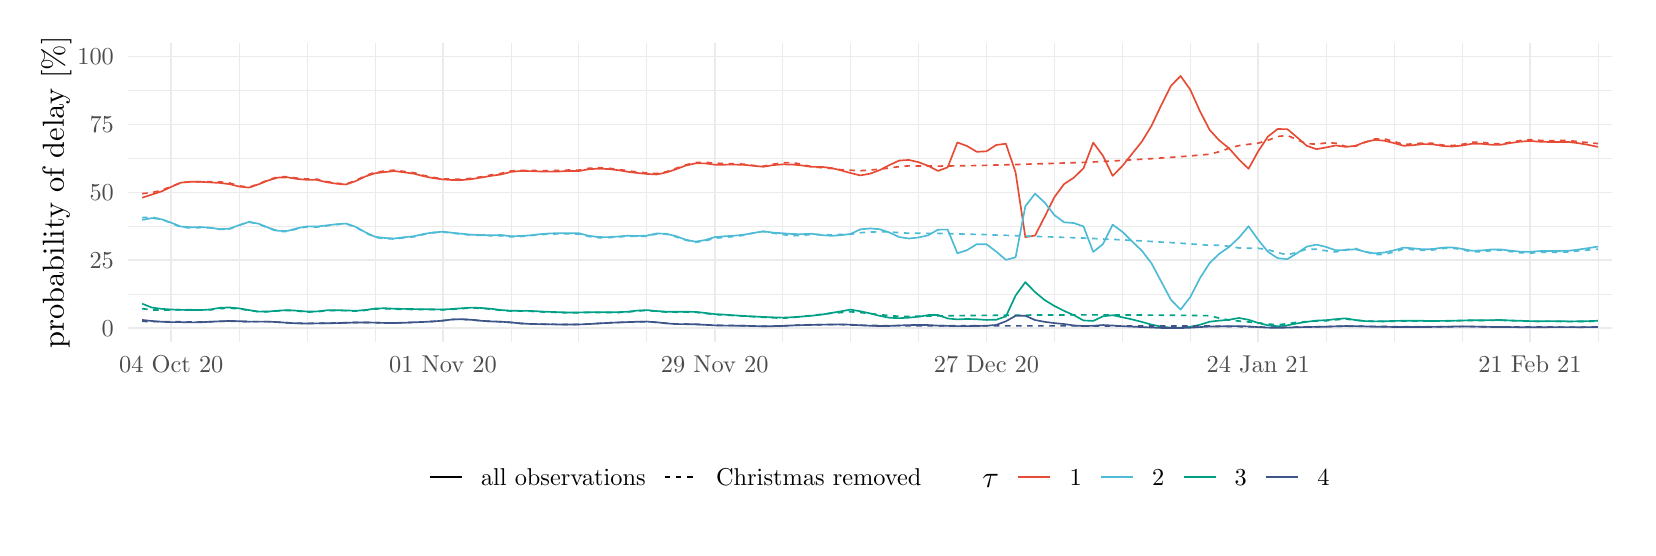
\begin{tikzpicture}[x=1pt,y=1pt]
\definecolor{fillColor}{RGB}{255,255,255}
\path[use as bounding box,fill=fillColor,fill opacity=0.00] (0,0) rectangle (578.16,180.67);
\begin{scope}
\path[clip] ( 36.11, 67.14) rectangle (572.66,175.17);
\definecolor{drawColor}{gray}{0.92}

\path[draw=drawColor,line width= 0.3pt,line join=round] ( 36.11, 84.33) --
	(572.66, 84.33);

\path[draw=drawColor,line width= 0.3pt,line join=round] ( 36.11,108.88) --
	(572.66,108.88);

\path[draw=drawColor,line width= 0.3pt,line join=round] ( 36.11,133.43) --
	(572.66,133.43);

\path[draw=drawColor,line width= 0.3pt,line join=round] ( 36.11,157.99) --
	(572.66,157.99);

\path[draw=drawColor,line width= 0.3pt,line join=round] ( 76.44, 67.14) --
	( 76.44,175.17);

\path[draw=drawColor,line width= 0.3pt,line join=round] (100.99, 67.14) --
	(100.99,175.17);

\path[draw=drawColor,line width= 0.3pt,line join=round] (125.54, 67.14) --
	(125.54,175.17);

\path[draw=drawColor,line width= 0.3pt,line join=round] (174.63, 67.14) --
	(174.63,175.17);

\path[draw=drawColor,line width= 0.3pt,line join=round] (199.18, 67.14) --
	(199.18,175.17);

\path[draw=drawColor,line width= 0.3pt,line join=round] (223.73, 67.14) --
	(223.73,175.17);

\path[draw=drawColor,line width= 0.3pt,line join=round] (272.82, 67.14) --
	(272.82,175.17);

\path[draw=drawColor,line width= 0.3pt,line join=round] (297.37, 67.14) --
	(297.37,175.17);

\path[draw=drawColor,line width= 0.3pt,line join=round] (321.92, 67.14) --
	(321.92,175.17);

\path[draw=drawColor,line width= 0.3pt,line join=round] (371.02, 67.14) --
	(371.02,175.17);

\path[draw=drawColor,line width= 0.3pt,line join=round] (395.56, 67.14) --
	(395.56,175.17);

\path[draw=drawColor,line width= 0.3pt,line join=round] (420.11, 67.14) --
	(420.11,175.17);

\path[draw=drawColor,line width= 0.3pt,line join=round] (469.21, 67.14) --
	(469.21,175.17);

\path[draw=drawColor,line width= 0.3pt,line join=round] (493.76, 67.14) --
	(493.76,175.17);

\path[draw=drawColor,line width= 0.3pt,line join=round] (518.30, 67.14) --
	(518.30,175.17);

\path[draw=drawColor,line width= 0.3pt,line join=round] (567.40, 67.14) --
	(567.40,175.17);

\path[draw=drawColor,line width= 0.6pt,line join=round] ( 36.11, 72.05) --
	(572.66, 72.05);

\path[draw=drawColor,line width= 0.6pt,line join=round] ( 36.11, 96.60) --
	(572.66, 96.60);

\path[draw=drawColor,line width= 0.6pt,line join=round] ( 36.11,121.16) --
	(572.66,121.16);

\path[draw=drawColor,line width= 0.6pt,line join=round] ( 36.11,145.71) --
	(572.66,145.71);

\path[draw=drawColor,line width= 0.6pt,line join=round] ( 36.11,170.26) --
	(572.66,170.26);

\path[draw=drawColor,line width= 0.6pt,line join=round] ( 51.89, 67.14) --
	( 51.89,175.17);

\path[draw=drawColor,line width= 0.6pt,line join=round] (150.08, 67.14) --
	(150.08,175.17);

\path[draw=drawColor,line width= 0.6pt,line join=round] (248.28, 67.14) --
	(248.28,175.17);

\path[draw=drawColor,line width= 0.6pt,line join=round] (346.47, 67.14) --
	(346.47,175.17);

\path[draw=drawColor,line width= 0.6pt,line join=round] (444.66, 67.14) --
	(444.66,175.17);

\path[draw=drawColor,line width= 0.6pt,line join=round] (542.85, 67.14) --
	(542.85,175.17);
\definecolor{drawColor}{RGB}{230,75,53}

\path[draw=drawColor,line width= 0.6pt,line join=round] ( 41.37,119.23) --
	( 44.88,120.36) --
	( 48.39,121.51) --
	( 51.89,123.15) --
	( 55.40,124.67) --
	( 58.91,125.01) --
	( 62.41,124.97) --
	( 65.92,124.76) --
	( 69.43,124.56) --
	( 72.93,124.13) --
	( 76.44,123.25) --
	( 79.95,122.89) --
	( 83.45,124.06) --
	( 86.96,125.48) --
	( 90.47,126.50) --
	( 93.97,126.57) --
	( 97.48,125.99) --
	(100.99,125.69) --
	(104.49,125.66) --
	(108.00,124.83) --
	(111.51,124.29) --
	(115.02,124.01) --
	(118.52,125.23) --
	(122.03,126.90) --
	(125.54,128.06) --
	(129.04,128.49) --
	(132.55,128.86) --
	(136.06,128.38) --
	(139.56,127.92) --
	(143.07,126.99) --
	(146.58,126.30) --
	(150.08,125.83) --
	(153.59,125.61) --
	(157.10,125.62) --
	(160.60,125.97) --
	(164.11,126.55) --
	(167.62,127.15) --
	(171.13,127.64) --
	(174.63,128.56) --
	(178.14,128.88) --
	(181.65,128.84) --
	(185.15,128.70) --
	(188.66,128.65) --
	(192.17,128.72) --
	(195.67,128.87) --
	(199.18,128.84) --
	(202.69,129.51) --
	(206.19,129.72) --
	(209.70,129.59) --
	(213.21,129.21) --
	(216.71,128.61) --
	(220.22,128.16) --
	(223.73,127.82) --
	(227.23,127.62) --
	(230.74,128.34) --
	(234.25,129.51) --
	(237.76,130.83) --
	(241.26,131.62) --
	(244.77,131.63) --
	(248.28,131.16) --
	(251.78,131.16) --
	(255.29,131.19) --
	(258.80,131.11) --
	(262.30,130.76) --
	(265.81,130.41) --
	(269.32,130.99) --
	(272.82,131.27) --
	(276.33,131.22) --
	(279.84,130.87) --
	(283.34,130.36) --
	(286.85,130.37) --
	(290.36,129.97) --
	(293.87,129.11) --
	(297.37,128.14) --
	(300.88,127.28) --
	(304.39,127.90) --
	(307.89,129.20) --
	(311.40,131.03) --
	(314.91,132.65) --
	(318.41,132.87) --
	(321.92,132.07) --
	(325.43,130.73) --
	(328.93,128.90) --
	(332.44,130.21) --
	(335.95,139.20) --
	(339.45,137.89) --
	(342.96,135.81) --
	(346.47,135.99) --
	(349.97,138.27) --
	(353.48,138.74) --
	(356.99,128.29) --
	(360.50,104.99) --
	(364.00,105.54) --
	(367.51,112.36) --
	(371.02,119.47) --
	(374.52,124.18) --
	(378.03,126.48) --
	(381.54,129.90) --
	(385.04,139.13) --
	(388.55,134.37) --
	(392.06,127.12) --
	(395.56,130.70) --
	(399.07,135.09) --
	(402.58,139.47) --
	(406.08,145.19) --
	(409.59,152.63) --
	(413.10,159.64) --
	(416.60,163.22) --
	(420.11,158.25) --
	(423.62,150.43) --
	(427.13,143.67) --
	(430.63,139.88) --
	(434.14,137.06) --
	(437.65,133.06) --
	(441.15,129.68) --
	(444.66,136.03) --
	(448.17,141.33) --
	(451.67,144.04) --
	(455.18,144.00) --
	(458.69,141.05) --
	(462.19,137.98) --
	(465.70,136.77) --
	(469.21,137.39) --
	(472.71,138.11) --
	(476.22,137.59) --
	(479.73,137.98) --
	(483.24,139.33) --
	(486.74,140.12) --
	(490.25,139.82) --
	(493.76,138.96) --
	(497.26,137.97) --
	(500.77,138.22) --
	(504.28,138.61) --
	(507.78,138.51) --
	(511.29,137.92) --
	(514.80,137.72) --
	(518.30,138.08) --
	(521.81,138.70) --
	(525.32,138.71) --
	(528.82,138.37) --
	(532.33,138.37) --
	(535.84,139.00) --
	(539.34,139.48) --
	(542.85,139.74) --
	(546.36,139.46) --
	(549.87,139.36) --
	(553.37,139.36) --
	(556.88,139.36) --
	(560.39,138.92) --
	(563.89,138.33) --
	(567.40,137.58);

\path[draw=drawColor,line width= 0.6pt,dash pattern=on 2pt off 2pt ,line join=round] ( 41.37,120.70) --
	( 44.88,121.07) --
	( 48.39,121.92) --
	( 51.89,123.30) --
	( 55.40,124.68) --
	( 58.91,124.97) --
	( 62.41,125.01) --
	( 65.92,124.99) --
	( 69.43,124.96) --
	( 72.93,124.55) --
	( 76.44,123.52) --
	( 79.95,122.99) --
	( 83.45,124.23) --
	( 86.96,125.68) --
	( 90.47,126.79) --
	( 93.97,126.84) --
	( 97.48,126.26) --
	(100.99,125.97) --
	(104.49,125.93) --
	(108.00,125.07) --
	(111.51,124.48) --
	(115.02,124.13) --
	(118.52,125.46) --
	(122.03,127.18) --
	(125.54,128.43) --
	(129.04,128.86) --
	(132.55,129.18) --
	(136.06,128.70) --
	(139.56,128.26) --
	(143.07,127.27) --
	(146.58,126.56) --
	(150.08,126.04) --
	(153.59,125.90) --
	(157.10,125.90) --
	(160.60,126.28) --
	(164.11,126.81) --
	(167.62,127.49) --
	(171.13,128.04) --
	(174.63,128.90) --
	(178.14,129.12) --
	(181.65,129.08) --
	(185.15,128.99) --
	(188.66,129.01) --
	(192.17,129.06) --
	(195.67,129.23) --
	(199.18,129.20) --
	(202.69,129.85) --
	(206.19,130.07) --
	(209.70,129.90) --
	(213.21,129.49) --
	(216.71,128.98) --
	(220.22,128.51) --
	(223.73,128.19) --
	(227.23,127.95) --
	(230.74,128.60) --
	(234.25,129.84) --
	(237.76,131.08) --
	(241.26,131.96) --
	(244.77,132.02) --
	(248.28,131.70) --
	(251.78,131.58) --
	(255.29,131.53) --
	(258.80,131.33) --
	(262.30,130.85) --
	(265.81,130.61) --
	(269.32,131.33) --
	(272.82,131.86) --
	(276.33,131.93) --
	(279.84,131.25) --
	(283.34,130.42) --
	(286.85,130.08) --
	(290.36,129.81) --
	(293.87,129.34) --
	(297.37,129.14) --
	(300.88,128.97) --
	(304.39,129.23) --
	(307.89,129.51) --
	(311.40,129.97) --
	(314.91,130.46) --
	(318.41,130.74) --
	(321.92,130.70) --
	(325.43,130.67) --
	(328.93,130.64) --
	(332.44,130.68) --
	(335.95,130.75) --
	(339.45,130.79) --
	(342.96,130.85) --
	(346.47,130.92) --
	(349.97,131.04) --
	(353.48,131.11) --
	(356.99,131.21) --
	(360.50,131.33) --
	(364.00,131.44) --
	(367.51,131.54) --
	(371.02,131.64) --
	(374.52,131.76) --
	(378.03,131.87) --
	(381.54,131.99) --
	(385.04,132.14) --
	(388.55,132.35) --
	(392.06,132.51) --
	(395.56,132.69) --
	(399.07,132.92) --
	(402.58,133.13) --
	(406.08,133.33) --
	(409.59,133.58) --
	(413.10,133.80) --
	(416.60,134.06) --
	(420.11,134.34) --
	(423.62,134.63) --
	(427.13,134.95) --
	(430.63,135.86) --
	(434.14,137.08) --
	(437.65,138.05) --
	(441.15,138.53) --
	(444.66,138.95) --
	(448.17,139.97) --
	(451.67,141.34) --
	(455.18,141.75) --
	(458.69,140.18) --
	(462.19,138.73) --
	(465.70,138.60) --
	(469.21,139.01) --
	(472.71,138.95) --
	(476.22,137.77) --
	(479.73,137.78) --
	(483.24,139.23) --
	(486.74,140.48) --
	(490.25,140.47) --
	(493.76,139.54) --
	(497.26,138.43) --
	(500.77,138.72) --
	(504.28,138.99) --
	(507.78,138.87) --
	(511.29,138.25) --
	(514.80,138.06) --
	(518.30,138.49) --
	(521.81,139.24) --
	(525.32,139.25) --
	(528.82,138.83) --
	(532.33,138.68) --
	(535.84,139.31) --
	(539.34,139.89) --
	(542.85,140.20) --
	(546.36,139.95) --
	(549.87,139.82) --
	(553.37,139.90) --
	(556.88,139.86) --
	(560.39,139.48) --
	(563.89,139.12) --
	(567.40,138.79);
\definecolor{drawColor}{RGB}{77,187,213}

\path[draw=drawColor,line width= 0.6pt,line join=round] ( 41.37,111.21) --
	( 44.88,111.85) --
	( 48.39,111.43) --
	( 51.89,110.18) --
	( 55.40,108.79) --
	( 58.91,108.56) --
	( 62.41,108.62) --
	( 65.92,108.40) --
	( 69.43,107.85) --
	( 72.93,108.03) --
	( 76.44,109.34) --
	( 79.95,110.47) --
	( 83.45,109.83) --
	( 86.96,108.39) --
	( 90.47,107.24) --
	( 93.97,107.23) --
	( 97.48,108.21) --
	(100.99,108.88) --
	(104.49,108.81) --
	(108.00,109.21) --
	(111.51,109.64) --
	(115.02,109.88) --
	(118.52,108.71) --
	(122.03,106.73) --
	(125.54,105.10) --
	(129.04,104.67) --
	(132.55,104.49) --
	(136.06,104.96) --
	(139.56,105.31) --
	(143.07,106.11) --
	(146.58,106.69) --
	(150.08,106.94) --
	(153.59,106.53) --
	(157.10,106.18) --
	(160.60,105.84) --
	(164.11,105.75) --
	(167.62,105.67) --
	(171.13,105.74) --
	(174.63,105.31) --
	(178.14,105.39) --
	(181.65,105.65) --
	(185.15,106.05) --
	(188.66,106.32) --
	(192.17,106.42) --
	(195.67,106.39) --
	(199.18,106.39) --
	(202.69,105.48) --
	(206.19,105.01) --
	(209.70,104.98) --
	(213.21,105.19) --
	(216.71,105.50) --
	(220.22,105.41) --
	(223.73,105.51) --
	(227.23,106.31) --
	(230.74,106.19) --
	(234.25,105.34) --
	(237.76,104.06) --
	(241.26,103.35) --
	(244.77,103.92) --
	(248.28,104.99) --
	(251.78,105.28) --
	(255.29,105.50) --
	(258.80,105.85) --
	(262.30,106.50) --
	(265.81,107.09) --
	(269.32,106.62) --
	(272.82,106.37) --
	(276.33,106.10) --
	(279.84,106.06) --
	(283.34,106.20) --
	(286.85,105.71) --
	(290.36,105.46) --
	(293.87,105.67) --
	(297.37,106.15) --
	(300.88,107.80) --
	(304.39,108.12) --
	(307.89,107.84) --
	(311.40,106.65) --
	(314.91,105.01) --
	(318.41,104.48) --
	(321.92,104.85) --
	(325.43,105.66) --
	(328.93,107.67) --
	(332.44,107.71) --
	(335.95, 99.14) --
	(339.45,100.28) --
	(342.96,102.44) --
	(346.47,102.41) --
	(349.97, 99.77) --
	(353.48, 96.77) --
	(356.99, 97.70) --
	(360.50,116.12) --
	(364.00,120.70) --
	(367.51,117.46) --
	(371.02,112.93) --
	(374.52,110.34) --
	(378.03,110.08) --
	(381.54,108.83) --
	(385.04, 99.63) --
	(388.55,102.47) --
	(392.06,109.49) --
	(395.56,106.91) --
	(399.07,103.43) --
	(402.58,100.12) --
	(406.08, 95.53) --
	(409.59, 88.96) --
	(413.10, 82.37) --
	(416.60, 78.78) --
	(420.11, 83.32) --
	(423.62, 90.18) --
	(427.13, 95.66) --
	(430.63, 99.00) --
	(434.14,101.44) --
	(437.65,104.74) --
	(441.15,108.91) --
	(444.66,103.97) --
	(448.17, 99.68) --
	(451.67, 97.38) --
	(455.18, 97.01) --
	(458.69, 99.17) --
	(462.19,101.55) --
	(465.70,102.28) --
	(469.21,101.42) --
	(472.71,100.21) --
	(476.22,100.33) --
	(479.73,100.60) --
	(483.24, 99.72) --
	(486.74, 99.11) --
	(490.25, 99.43) --
	(493.76,100.23) --
	(497.26,101.20) --
	(500.77,100.91) --
	(504.28,100.57) --
	(507.78,100.69) --
	(511.29,101.19) --
	(514.80,101.27) --
	(518.30,100.74) --
	(521.81,100.08) --
	(525.32,100.15) --
	(528.82,100.52) --
	(532.33,100.54) --
	(535.84,100.08) --
	(539.34, 99.74) --
	(542.85, 99.66) --
	(546.36, 99.94) --
	(549.87, 99.98) --
	(553.37, 99.99) --
	(556.88,100.05) --
	(560.39,100.49) --
	(563.89,101.00) --
	(567.40,101.57);

\path[draw=drawColor,line width= 0.6pt,dash pattern=on 2pt off 2pt ,line join=round] ( 41.37,112.03) --
	( 44.88,112.19) --
	( 48.39,111.45) --
	( 51.89,110.03) --
	( 55.40,108.55) --
	( 58.91,108.30) --
	( 62.41,108.41) --
	( 65.92,108.32) --
	( 69.43,107.78) --
	( 72.93,107.94) --
	( 76.44,109.28) --
	( 79.95,110.46) --
	( 83.45,109.72) --
	( 86.96,108.24) --
	( 90.47,107.02) --
	( 93.97,107.05) --
	( 97.48,108.02) --
	(100.99,108.70) --
	(104.49,108.61) --
	(108.00,109.06) --
	(111.51,109.51) --
	(115.02,109.84) --
	(118.52,108.58) --
	(122.03,106.58) --
	(125.54,104.88) --
	(129.04,104.46) --
	(132.55,104.29) --
	(136.06,104.75) --
	(139.56,105.10) --
	(143.07,105.94) --
	(146.58,106.55) --
	(150.08,106.83) --
	(153.59,106.39) --
	(157.10,106.04) --
	(160.60,105.66) --
	(164.11,105.62) --
	(167.62,105.47) --
	(171.13,105.46) --
	(174.63,105.08) --
	(178.14,105.23) --
	(181.65,105.53) --
	(185.15,105.88) --
	(188.66,106.06) --
	(192.17,106.19) --
	(195.67,106.15) --
	(199.18,106.13) --
	(202.69,105.23) --
	(206.19,104.78) --
	(209.70,104.78) --
	(213.21,105.04) --
	(216.71,105.28) --
	(220.22,105.23) --
	(223.73,105.32) --
	(227.23,106.11) --
	(230.74,106.05) --
	(234.25,105.11) --
	(237.76,103.89) --
	(241.26,103.11) --
	(244.77,103.63) --
	(248.28,104.55) --
	(251.78,104.92) --
	(255.29,105.21) --
	(258.80,105.65) --
	(262.30,106.47) --
	(265.81,107.00) --
	(269.32,106.44) --
	(272.82,105.93) --
	(276.33,105.47) --
	(279.84,105.62) --
	(283.34,105.99) --
	(286.85,105.88) --
	(290.36,105.78) --
	(293.87,105.98) --
	(297.37,105.99) --
	(300.88,106.58) --
	(304.39,106.79) --
	(307.89,106.93) --
	(311.40,106.84) --
	(314.91,106.60) --
	(318.41,106.38) --
	(321.92,106.36) --
	(325.43,106.35) --
	(328.93,106.33) --
	(332.44,106.25) --
	(335.95,106.13) --
	(339.45,106.05) --
	(342.96,105.96) --
	(346.47,105.88) --
	(349.97,105.72) --
	(353.48,105.63) --
	(356.99,105.50) --
	(360.50,105.37) --
	(364.00,105.24) --
	(367.51,105.12) --
	(371.02,105.02) --
	(374.52,104.88) --
	(378.03,104.77) --
	(381.54,104.65) --
	(385.04,104.49) --
	(388.55,104.29) --
	(392.06,104.16) --
	(395.56,103.99) --
	(399.07,103.79) --
	(402.58,103.60) --
	(406.08,103.42) --
	(409.59,103.19) --
	(413.10,103.01) --
	(416.60,102.79) --
	(420.11,102.54) --
	(423.62,102.29) --
	(427.13,102.02) --
	(430.63,102.09) --
	(434.14,101.66) --
	(437.65,101.08) --
	(441.15,100.97) --
	(444.66,100.95) --
	(448.17,100.44) --
	(451.67, 99.41) --
	(455.18, 98.56) --
	(458.69, 99.52) --
	(462.19,100.67) --
	(465.70,100.59) --
	(469.21,100.04) --
	(472.71, 99.64) --
	(476.22,100.44) --
	(479.73,100.86) --
	(483.24, 99.77) --
	(486.74, 98.70) --
	(490.25, 98.75) --
	(493.76, 99.62) --
	(497.26,100.74) --
	(500.77,100.43) --
	(504.28,100.21) --
	(507.78,100.36) --
	(511.29,100.89) --
	(514.80,101.01) --
	(518.30,100.47) --
	(521.81, 99.65) --
	(525.32, 99.69) --
	(528.82,100.11) --
	(532.33,100.25) --
	(535.84, 99.76) --
	(539.34, 99.32) --
	(542.85, 99.20) --
	(546.36, 99.46) --
	(549.87, 99.56) --
	(553.37, 99.51) --
	(556.88, 99.63) --
	(560.39,100.01) --
	(563.89,100.34) --
	(567.40,100.59);
\definecolor{drawColor}{RGB}{0,160,135}

\path[draw=drawColor,line width= 0.6pt,line join=round] ( 41.37, 80.92) --
	( 44.88, 79.53) --
	( 48.39, 79.06) --
	( 51.89, 78.83) --
	( 55.40, 78.69) --
	( 58.91, 78.66) --
	( 62.41, 78.61) --
	( 65.92, 78.85) --
	( 69.43, 79.43) --
	( 72.93, 79.58) --
	( 76.44, 79.23) --
	( 79.95, 78.62) --
	( 83.45, 78.07) --
	( 86.96, 78.10) --
	( 90.47, 78.41) --
	( 93.97, 78.61) --
	( 97.48, 78.40) --
	(100.99, 78.09) --
	(104.49, 78.14) --
	(108.00, 78.53) --
	(111.51, 78.58) --
	(115.02, 78.51) --
	(118.52, 78.35) --
	(122.03, 78.65) --
	(125.54, 79.17) --
	(129.04, 79.29) --
	(132.55, 79.11) --
	(136.06, 79.05) --
	(139.56, 78.98) --
	(143.07, 78.97) --
	(146.58, 78.90) --
	(150.08, 78.84) --
	(153.59, 79.03) --
	(157.10, 79.30) --
	(160.60, 79.52) --
	(164.11, 79.37) --
	(167.62, 79.07) --
	(171.13, 78.63) --
	(174.63, 78.39) --
	(178.14, 78.35) --
	(181.65, 78.32) --
	(185.15, 78.13) --
	(188.66, 77.98) --
	(192.17, 77.86) --
	(195.67, 77.76) --
	(199.18, 77.77) --
	(202.69, 77.85) --
	(206.19, 77.89) --
	(209.70, 77.86) --
	(213.21, 77.87) --
	(216.71, 78.02) --
	(220.22, 78.43) --
	(223.73, 78.61) --
	(227.23, 78.27) --
	(230.74, 78.05) --
	(234.25, 77.99) --
	(237.76, 78.00) --
	(241.26, 77.98) --
	(244.77, 77.59) --
	(248.28, 77.17) --
	(251.78, 76.97) --
	(255.29, 76.73) --
	(258.80, 76.50) --
	(262.30, 76.31) --
	(265.81, 76.14) --
	(269.32, 76.00) --
	(272.82, 75.89) --
	(276.33, 76.03) --
	(279.84, 76.29) --
	(283.34, 76.58) --
	(286.85, 76.98) --
	(290.36, 77.57) --
	(293.87, 78.18) --
	(297.37, 78.79) --
	(300.88, 78.19) --
	(304.39, 77.43) --
	(307.89, 76.52) --
	(311.40, 75.85) --
	(314.91, 75.69) --
	(318.41, 75.88) --
	(321.92, 76.22) --
	(325.43, 76.82) --
	(328.93, 76.85) --
	(332.44, 75.59) --
	(335.95, 75.25) --
	(339.45, 75.41) --
	(342.96, 75.29) --
	(346.47, 75.06) --
	(349.97, 75.13) --
	(353.48, 76.33) --
	(356.99, 83.88) --
	(360.50, 88.72) --
	(364.00, 85.14) --
	(367.51, 82.23) --
	(371.02, 80.09) --
	(374.52, 78.33) --
	(378.03, 76.78) --
	(381.54, 74.86) --
	(385.04, 74.71) --
	(388.55, 76.37) --
	(392.06, 76.77) --
	(395.56, 76.01) --
	(399.07, 75.25) --
	(402.58, 74.35) --
	(406.08, 73.38) --
	(409.59, 72.65) --
	(413.10, 72.28) --
	(416.60, 72.28) --
	(420.11, 72.59) --
	(423.62, 73.32) --
	(427.13, 74.42) --
	(430.63, 74.82) --
	(434.14, 75.12) --
	(437.65, 75.77) --
	(441.15, 75.12) --
	(444.66, 73.96) --
	(448.17, 73.13) --
	(451.67, 72.77) --
	(455.18, 73.12) --
	(458.69, 73.80) --
	(462.19, 74.38) --
	(465.70, 74.82) --
	(469.21, 74.97) --
	(472.71, 75.34) --
	(476.22, 75.64) --
	(479.73, 75.03) --
	(483.24, 74.64) --
	(486.74, 74.55) --
	(490.25, 74.57) --
	(493.76, 74.71) --
	(497.26, 74.75) --
	(500.77, 74.80) --
	(504.28, 74.74) --
	(507.78, 74.67) --
	(511.29, 74.72) --
	(514.80, 74.77) --
	(518.30, 74.86) --
	(521.81, 74.95) --
	(525.32, 74.96) --
	(528.82, 74.99) --
	(532.33, 75.03) --
	(535.84, 74.86) --
	(539.34, 74.77) --
	(542.85, 74.63) --
	(546.36, 74.60) --
	(549.87, 74.63) --
	(553.37, 74.60) --
	(556.88, 74.54) --
	(560.39, 74.56) --
	(563.89, 74.63) --
	(567.40, 74.76);

\path[draw=drawColor,line width= 0.6pt,dash pattern=on 2pt off 2pt ,line join=round] ( 41.37, 79.14) --
	( 44.88, 78.67) --
	( 48.39, 78.63) --
	( 51.89, 78.69) --
	( 55.40, 78.76) --
	( 58.91, 78.80) --
	( 62.41, 78.67) --
	( 65.92, 78.69) --
	( 69.43, 79.15) --
	( 72.93, 79.31) --
	( 76.44, 79.06) --
	( 79.95, 78.52) --
	( 83.45, 78.01) --
	( 86.96, 78.05) --
	( 90.47, 78.34) --
	( 93.97, 78.49) --
	( 97.48, 78.27) --
	(100.99, 77.93) --
	(104.49, 78.01) --
	(108.00, 78.39) --
	(111.51, 78.48) --
	(115.02, 78.40) --
	(118.52, 78.23) --
	(122.03, 78.53) --
	(125.54, 79.02) --
	(129.04, 79.12) --
	(132.55, 78.96) --
	(136.06, 78.91) --
	(139.56, 78.83) --
	(143.07, 78.84) --
	(146.58, 78.77) --
	(150.08, 78.73) --
	(153.59, 78.89) --
	(157.10, 79.18) --
	(160.60, 79.39) --
	(164.11, 79.25) --
	(167.62, 78.94) --
	(171.13, 78.50) --
	(174.63, 78.28) --
	(178.14, 78.25) --
	(181.65, 78.18) --
	(185.15, 77.99) --
	(188.66, 77.85) --
	(192.17, 77.72) --
	(195.67, 77.63) --
	(199.18, 77.63) --
	(202.69, 77.74) --
	(206.19, 77.77) --
	(209.70, 77.74) --
	(213.21, 77.74) --
	(216.71, 77.90) --
	(220.22, 78.31) --
	(223.73, 78.50) --
	(227.23, 78.17) --
	(230.74, 77.92) --
	(234.25, 77.86) --
	(237.76, 77.87) --
	(241.26, 77.84) --
	(244.77, 77.44) --
	(248.28, 77.02) --
	(251.78, 76.86) --
	(255.29, 76.64) --
	(258.80, 76.46) --
	(262.30, 76.24) --
	(265.81, 76.01) --
	(269.32, 75.83) --
	(272.82, 75.70) --
	(276.33, 75.92) --
	(279.84, 76.31) --
	(283.34, 76.69) --
	(286.85, 77.09) --
	(290.36, 77.47) --
	(293.87, 77.73) --
	(297.37, 78.01) --
	(300.88, 77.73) --
	(304.39, 77.35) --
	(307.89, 76.96) --
	(311.40, 76.61) --
	(314.91, 76.37) --
	(318.41, 76.35) --
	(321.92, 76.41) --
	(325.43, 76.46) --
	(328.93, 76.51) --
	(332.44, 76.55) --
	(335.95, 76.60) --
	(339.45, 76.65) --
	(342.96, 76.68) --
	(346.47, 76.70) --
	(349.97, 76.73) --
	(353.48, 76.76) --
	(356.99, 76.79) --
	(360.50, 76.80) --
	(364.00, 76.83) --
	(367.51, 76.84) --
	(371.02, 76.85) --
	(374.52, 76.87) --
	(378.03, 76.88) --
	(381.54, 76.88) --
	(385.04, 76.89) --
	(388.55, 76.88) --
	(392.06, 76.87) --
	(395.56, 76.85) --
	(399.07, 76.83) --
	(402.58, 76.82) --
	(406.08, 76.80) --
	(409.59, 76.78) --
	(413.10, 76.75) --
	(416.60, 76.71) --
	(420.11, 76.68) --
	(423.62, 76.64) --
	(427.13, 76.59) --
	(430.63, 75.69) --
	(434.14, 75.00) --
	(437.65, 74.66) --
	(441.15, 74.33) --
	(444.66, 74.00) --
	(448.17, 73.59) --
	(451.67, 73.29) --
	(455.18, 73.69) --
	(458.69, 74.22) --
	(462.19, 74.45) --
	(465.70, 74.66) --
	(469.21, 74.75) --
	(472.71, 75.11) --
	(476.22, 75.41) --
	(479.73, 74.98) --
	(483.24, 74.67) --
	(486.74, 74.56) --
	(490.25, 74.51) --
	(493.76, 74.61) --
	(497.26, 74.63) --
	(500.77, 74.68) --
	(504.28, 74.64) --
	(507.78, 74.61) --
	(511.29, 74.68) --
	(514.80, 74.72) --
	(518.30, 74.81) --
	(521.81, 74.88) --
	(525.32, 74.87) --
	(528.82, 74.90) --
	(532.33, 74.94) --
	(535.84, 74.79) --
	(539.34, 74.70) --
	(542.85, 74.54) --
	(546.36, 74.52) --
	(549.87, 74.55) --
	(553.37, 74.53) --
	(556.88, 74.46) --
	(560.39, 74.48) --
	(563.89, 74.51) --
	(567.40, 74.57);
\definecolor{drawColor}{RGB}{60,84,136}

\path[draw=drawColor,line width= 0.6pt,line join=round] ( 41.37, 75.05) --
	( 44.88, 74.67) --
	( 48.39, 74.41) --
	( 51.89, 74.26) --
	( 55.40, 74.26) --
	( 58.91, 74.18) --
	( 62.41, 74.21) --
	( 65.92, 74.40) --
	( 69.43, 74.57) --
	( 72.93, 74.69) --
	( 76.44, 74.60) --
	( 79.95, 74.43) --
	( 83.45, 74.46) --
	( 86.96, 74.44) --
	( 90.47, 74.26) --
	( 93.97, 74.01) --
	( 97.48, 73.82) --
	(100.99, 73.76) --
	(104.49, 73.82) --
	(108.00, 73.85) --
	(111.51, 73.90) --
	(115.02, 74.02) --
	(118.52, 74.13) --
	(122.03, 74.13) --
	(125.54, 74.09) --
	(129.04, 73.97) --
	(132.55, 73.96) --
	(136.06, 74.03) --
	(139.56, 74.20) --
	(143.07, 74.34) --
	(146.58, 74.52) --
	(150.08, 74.81) --
	(153.59, 75.25) --
	(157.10, 75.30) --
	(160.60, 75.09) --
	(164.11, 74.73) --
	(167.62, 74.52) --
	(171.13, 74.41) --
	(174.63, 74.16) --
	(178.14, 73.80) --
	(181.65, 73.61) --
	(185.15, 73.54) --
	(188.66, 73.47) --
	(192.17, 73.42) --
	(195.67, 73.38) --
	(199.18, 73.42) --
	(202.69, 73.56) --
	(206.19, 73.79) --
	(209.70, 73.99) --
	(213.21, 74.15) --
	(216.71, 74.28) --
	(220.22, 74.41) --
	(223.73, 74.47) --
	(227.23, 74.21) --
	(230.74, 73.83) --
	(234.25, 73.57) --
	(237.76, 73.53) --
	(241.26, 73.47) --
	(244.77, 73.28) --
	(248.28, 73.09) --
	(251.78, 73.01) --
	(255.29, 72.99) --
	(258.80, 72.95) --
	(262.30, 72.84) --
	(265.81, 72.78) --
	(269.32, 72.80) --
	(272.82, 72.89) --
	(276.33, 73.07) --
	(279.84, 73.19) --
	(283.34, 73.26) --
	(286.85, 73.35) --
	(290.36, 73.41) --
	(293.87, 73.46) --
	(297.37, 73.34) --
	(300.88, 73.14) --
	(304.39, 72.96) --
	(307.89, 72.86) --
	(311.40, 72.89) --
	(314.91, 73.06) --
	(318.41, 73.18) --
	(321.92, 73.27) --
	(325.43, 73.21) --
	(328.93, 73.00) --
	(332.44, 72.91) --
	(335.95, 72.82) --
	(339.45, 72.83) --
	(342.96, 72.87) --
	(346.47, 72.96) --
	(349.97, 73.24) --
	(353.48, 74.58) --
	(356.99, 76.55) --
	(360.50, 76.58) --
	(364.00, 75.03) --
	(367.51, 74.36) --
	(371.02, 73.92) --
	(374.52, 73.57) --
	(378.03, 73.07) --
	(381.54, 72.83) --
	(385.04, 72.95) --
	(388.55, 73.21) --
	(392.06, 73.04) --
	(395.56, 72.80) --
	(399.07, 72.64) --
	(402.58, 72.48) --
	(406.08, 72.32) --
	(409.59, 72.17) --
	(413.10, 72.12) --
	(416.60, 72.14) --
	(420.11, 72.25) --
	(423.62, 72.48) --
	(427.13, 72.67) --
	(430.63, 72.72) --
	(434.14, 72.80) --
	(437.65, 72.84) --
	(441.15, 72.71) --
	(444.66, 72.46) --
	(448.17, 72.27) --
	(451.67, 72.23) --
	(455.18, 72.28) --
	(458.69, 72.40) --
	(462.19, 72.52) --
	(465.70, 72.55) --
	(469.21, 72.63) --
	(472.71, 72.75) --
	(476.22, 72.85) --
	(479.73, 72.81) --
	(483.24, 72.72) --
	(486.74, 72.63) --
	(490.25, 72.60) --
	(493.76, 72.51) --
	(497.26, 72.51) --
	(500.77, 72.49) --
	(504.28, 72.50) --
	(507.78, 72.54) --
	(511.29, 72.58) --
	(514.80, 72.66) --
	(518.30, 72.73) --
	(521.81, 72.68) --
	(525.32, 72.60) --
	(528.82, 72.53) --
	(532.33, 72.48) --
	(535.84, 72.48) --
	(539.34, 72.43) --
	(542.85, 72.39) --
	(546.36, 72.42) --
	(549.87, 72.45) --
	(553.37, 72.47) --
	(556.88, 72.47) --
	(560.39, 72.44) --
	(563.89, 72.46) --
	(567.40, 72.51);

\path[draw=drawColor,line width= 0.6pt,dash pattern=on 2pt off 2pt ,line join=round] ( 41.37, 74.54) --
	( 44.88, 74.48) --
	( 48.39, 74.42) --
	( 51.89, 74.39) --
	( 55.40, 74.42) --
	( 58.91, 74.34) --
	( 62.41, 74.32) --
	( 65.92, 74.42) --
	( 69.43, 74.52) --
	( 72.93, 74.62) --
	( 76.44, 74.56) --
	( 79.95, 74.44) --
	( 83.45, 74.46) --
	( 86.96, 74.44) --
	( 90.47, 74.26) --
	( 93.97, 74.03) --
	( 97.48, 73.87) --
	(100.99, 73.81) --
	(104.49, 73.86) --
	(108.00, 73.89) --
	(111.51, 73.95) --
	(115.02, 74.05) --
	(118.52, 74.14) --
	(122.03, 74.12) --
	(125.54, 74.09) --
	(129.04, 73.98) --
	(132.55, 73.99) --
	(136.06, 74.06) --
	(139.56, 74.22) --
	(143.07, 74.36) --
	(146.58, 74.53) --
	(150.08, 74.82) --
	(153.59, 75.24) --
	(157.10, 75.29) --
	(160.60, 75.08) --
	(164.11, 74.73) --
	(167.62, 74.52) --
	(171.13, 74.41) --
	(174.63, 74.16) --
	(178.14, 73.81) --
	(181.65, 73.62) --
	(185.15, 73.56) --
	(188.66, 73.49) --
	(192.17, 73.44) --
	(195.67, 73.42) --
	(199.18, 73.45) --
	(202.69, 73.59) --
	(206.19, 73.80) --
	(209.70, 73.99) --
	(213.21, 74.14) --
	(216.71, 74.26) --
	(220.22, 74.37) --
	(223.73, 74.41) --
	(227.23, 74.19) --
	(230.74, 73.85) --
	(234.25, 73.61) --
	(237.76, 73.57) --
	(241.26, 73.51) --
	(244.77, 73.33) --
	(248.28, 73.14) --
	(251.78, 73.06) --
	(255.29, 73.03) --
	(258.80, 72.98) --
	(262.30, 72.86) --
	(265.81, 72.80) --
	(269.32, 72.82) --
	(272.82, 72.92) --
	(276.33, 73.10) --
	(279.84, 73.24) --
	(283.34, 73.31) --
	(286.85, 73.36) --
	(290.36, 73.36) --
	(293.87, 73.37) --
	(297.37, 73.27) --
	(300.88, 73.13) --
	(304.39, 73.05) --
	(307.89, 73.02) --
	(311.40, 73.00) --
	(314.91, 72.99) --
	(318.41, 72.95) --
	(321.92, 72.95) --
	(325.43, 72.94) --
	(328.93, 72.94) --
	(332.44, 72.94) --
	(335.95, 72.93) --
	(339.45, 72.93) --
	(342.96, 72.93) --
	(346.47, 72.92) --
	(349.97, 72.92) --
	(353.48, 72.92) --
	(356.99, 72.92) --
	(360.50, 72.91) --
	(364.00, 72.91) --
	(367.51, 72.91) --
	(371.02, 72.90) --
	(374.52, 72.90) --
	(378.03, 72.90) --
	(381.54, 72.90) --
	(385.04, 72.89) --
	(388.55, 72.89) --
	(392.06, 72.89) --
	(395.56, 72.88) --
	(399.07, 72.88) --
	(402.58, 72.88) --
	(406.08, 72.87) --
	(409.59, 72.87) --
	(413.10, 72.87) --
	(416.60, 72.86) --
	(420.11, 72.86) --
	(423.62, 72.86) --
	(427.13, 72.85) --
	(430.63, 72.77) --
	(434.14, 72.68) --
	(437.65, 72.63) --
	(441.15, 72.59) --
	(444.66, 72.52) --
	(448.17, 72.42) --
	(451.67, 72.37) --
	(455.18, 72.42) --
	(458.69, 72.49) --
	(462.19, 72.57) --
	(465.70, 72.57) --
	(469.21, 72.62) --
	(472.71, 72.71) --
	(476.22, 72.81) --
	(479.73, 72.79) --
	(483.24, 72.74) --
	(486.74, 72.68) --
	(490.25, 72.68) --
	(493.76, 72.64) --
	(497.26, 72.62) --
	(500.77, 72.58) --
	(504.28, 72.57) --
	(507.78, 72.58) --
	(511.29, 72.59) --
	(514.80, 72.62) --
	(518.30, 72.65) --
	(521.81, 72.64) --
	(525.32, 72.61) --
	(528.82, 72.57) --
	(532.33, 72.55) --
	(535.84, 72.55) --
	(539.34, 72.51) --
	(542.85, 72.48) --
	(546.36, 72.48) --
	(549.87, 72.49) --
	(553.37, 72.48) --
	(556.88, 72.46) --
	(560.39, 72.44) --
	(563.89, 72.45) --
	(567.40, 72.47);
\end{scope}
\begin{scope}
\path[clip] (  0.00,  0.00) rectangle (578.16,180.67);
\definecolor{drawColor}{gray}{0.30}

\node[text=drawColor,anchor=base east,inner sep=0pt, outer sep=0pt, scale=  0.88] at ( 31.16, 69.02) {0};

\node[text=drawColor,anchor=base east,inner sep=0pt, outer sep=0pt, scale=  0.88] at ( 31.16, 93.57) {25};

\node[text=drawColor,anchor=base east,inner sep=0pt, outer sep=0pt, scale=  0.88] at ( 31.16,118.13) {50};

\node[text=drawColor,anchor=base east,inner sep=0pt, outer sep=0pt, scale=  0.88] at ( 31.16,142.68) {75};

\node[text=drawColor,anchor=base east,inner sep=0pt, outer sep=0pt, scale=  0.88] at ( 31.16,167.23) {100};
\end{scope}
\begin{scope}
\path[clip] (  0.00,  0.00) rectangle (578.16,180.67);
\definecolor{drawColor}{gray}{0.30}

\node[text=drawColor,anchor=base,inner sep=0pt, outer sep=0pt, scale=  0.88] at ( 51.89, 56.13) {04 Oct 20};

\node[text=drawColor,anchor=base,inner sep=0pt, outer sep=0pt, scale=  0.88] at (150.08, 56.13) {01 Nov 20};

\node[text=drawColor,anchor=base,inner sep=0pt, outer sep=0pt, scale=  0.88] at (248.28, 56.13) {29 Nov 20};

\node[text=drawColor,anchor=base,inner sep=0pt, outer sep=0pt, scale=  0.88] at (346.47, 56.13) {27 Dec 20};

\node[text=drawColor,anchor=base,inner sep=0pt, outer sep=0pt, scale=  0.88] at (444.66, 56.13) {24 Jan 21};

\node[text=drawColor,anchor=base,inner sep=0pt, outer sep=0pt, scale=  0.88] at (542.85, 56.13) {21 Feb 21};
\end{scope}
\begin{scope}
\path[clip] (  0.00,  0.00) rectangle (578.16,180.67);
\definecolor{drawColor}{RGB}{0,0,0}

\node[text=drawColor,rotate= 90.00,anchor=base,inner sep=0pt, outer sep=0pt, scale=  1.10] at ( 13.08,121.16) {probability of delay [\%]};
\end{scope}
\begin{scope}
\path[clip] (  0.00,  0.00) rectangle (578.16,180.67);
\definecolor{drawColor}{RGB}{0,0,0}

\path[draw=drawColor,line width= 0.6pt,line join=round] (145.29, 18.23) -- (156.86, 18.23);
\end{scope}
\begin{scope}
\path[clip] (  0.00,  0.00) rectangle (578.16,180.67);
\definecolor{drawColor}{RGB}{0,0,0}

\path[draw=drawColor,line width= 0.6pt,dash pattern=on 2pt off 2pt ,line join=round] (230.25, 18.23) -- (241.82, 18.23);
\end{scope}
\begin{scope}
\path[clip] (  0.00,  0.00) rectangle (578.16,180.67);
\definecolor{drawColor}{RGB}{0,0,0}

\node[text=drawColor,anchor=base west,inner sep=0pt, outer sep=0pt, scale=  0.88] at (163.80, 15.20) {all observations};
\end{scope}
\begin{scope}
\path[clip] (  0.00,  0.00) rectangle (578.16,180.67);
\definecolor{drawColor}{RGB}{0,0,0}

\node[text=drawColor,anchor=base west,inner sep=0pt, outer sep=0pt, scale=  0.88] at (248.76, 15.20) {Christmas removed};
\end{scope}
\begin{scope}
\path[clip] (  0.00,  0.00) rectangle (578.16,180.67);
\definecolor{drawColor}{RGB}{0,0,0}

\node[text=drawColor,anchor=base west,inner sep=0pt, outer sep=0pt, scale=  1.10] at (344.96, 14.44) {$\tau$};
\end{scope}
\begin{scope}
\path[clip] (  0.00,  0.00) rectangle (578.16,180.67);
\definecolor{drawColor}{RGB}{230,75,53}

\path[draw=drawColor,line width= 0.6pt,line join=round] (357.96, 18.23) -- (369.52, 18.23);
\end{scope}
\begin{scope}
\path[clip] (  0.00,  0.00) rectangle (578.16,180.67);
\definecolor{drawColor}{RGB}{77,187,213}

\path[draw=drawColor,line width= 0.6pt,line join=round] (387.81, 18.23) -- (399.37, 18.23);
\end{scope}
\begin{scope}
\path[clip] (  0.00,  0.00) rectangle (578.16,180.67);
\definecolor{drawColor}{RGB}{0,160,135}

\path[draw=drawColor,line width= 0.6pt,line join=round] (417.66, 18.23) -- (429.23, 18.23);
\end{scope}
\begin{scope}
\path[clip] (  0.00,  0.00) rectangle (578.16,180.67);
\definecolor{drawColor}{RGB}{60,84,136}

\path[draw=drawColor,line width= 0.6pt,line join=round] (447.52, 18.23) -- (459.08, 18.23);
\end{scope}
\begin{scope}
\path[clip] (  0.00,  0.00) rectangle (578.16,180.67);
\definecolor{drawColor}{RGB}{0,0,0}

\node[text=drawColor,anchor=base west,inner sep=0pt, outer sep=0pt, scale=  0.88] at (376.47, 15.20) {1};
\end{scope}
\begin{scope}
\path[clip] (  0.00,  0.00) rectangle (578.16,180.67);
\definecolor{drawColor}{RGB}{0,0,0}

\node[text=drawColor,anchor=base west,inner sep=0pt, outer sep=0pt, scale=  0.88] at (406.32, 15.20) {2};
\end{scope}
\begin{scope}
\path[clip] (  0.00,  0.00) rectangle (578.16,180.67);
\definecolor{drawColor}{RGB}{0,0,0}

\node[text=drawColor,anchor=base west,inner sep=0pt, outer sep=0pt, scale=  0.88] at (436.17, 15.20) {3};
\end{scope}
\begin{scope}
\path[clip] (  0.00,  0.00) rectangle (578.16,180.67);
\definecolor{drawColor}{RGB}{0,0,0}

\node[text=drawColor,anchor=base west,inner sep=0pt, outer sep=0pt, scale=  0.88] at (466.03, 15.20) {4};
\end{scope}
\end{tikzpicture}
%
    }
    \caption{Importance sampling estimates of conditional expectation $\E \left( p_{t, \tau} | Y \right)$ for the two Christmas models. }
    \label{fig:christmas_delay_probs}
\end{figure}

\subsection{Discussion}
% extension: for true dealing with week-day effect, use information on symptom onset date
% extension: death data, both for forecasting and improving estimation
% extension: longer delays
% extension: keep number of cases in missing scenario constant
% extension: dark figure, w/deaths
% extension: weekday effects normalized like delays